% 
% (c) Copyright 2016 Tabea Mendez
% 
% This source is free: you can redistribute it and/or modify
% it under the terms of the GNU General Public License as published by
% the Free Software Foundation, either version 3 of the License, or
% (at your option) any later version.
% 
% This source is distributed in the hope that it will be useful,
% but WITHOUT ANY WARRANTY; without even the implied warranty of
% MERCHANTABILITY or FITNESS FOR A PARTICULAR PURPOSE.  See the
% GNU General Public License for more details.
% 
% You should have received a copy of the GNU General Public License
% along with this source.  If not, see <http://www.gnu.org/licenses/>.
%
%%%%%%%%%%%%%%%%%%%%%%%%%%%%%%%%%%%%%%%%%%%%%%%%%%%%%%%%%%%%%%%%%%%%%%%%%%%%%%

% % 
% (c) Copyright 2016 Tabea Mendez
% 
% This source is free: you can redistribute it and/or modify
% it under the terms of the GNU General Public License as published by
% the Free Software Foundation, either version 3 of the License, or
% (at your option) any later version.
% 
% This source is distributed in the hope that it will be useful,
% but WITHOUT ANY WARRANTY; without even the implied warranty of
% MERCHANTABILITY or FITNESS FOR A PARTICULAR PURPOSE.  See the
% GNU General Public License for more details.
% 
% You should have received a copy of the GNU General Public License
% along with this source.  If not, see <http://www.gnu.org/licenses/>.
%
%%%%%%%%%%%%%%%%%%%%%%%%%%%%%%%%%%%%%%%%%%%%%%%%%%%%%%%%%%%%%%%%%%%%%%%%%%%%%%

\chapter{Wahrscheinlichkeitsrechnung \small{\textcolor{black}{S.128}}}
	\section{Zufallsexperiment}
		\vspace*{-0.8cm}\begin{minipage}{0.4\textwidth}
			Ein Zufallsexperiment ist ein wiederholbares Experiment mit einem zufälligen Ergebnis.
		\end{minipage}
		\begin{minipage}{0.05\textwidth}$ $\end{minipage}
		\begin{minipage}{0.55\textwidth}
			\begin{tabular}{|c|}
			\hline\\[-0.4cm]
				Wiederholbares Experiment\\
				$\downarrow$\\
				Versuchsausgang (zufälliges Ergebnis)\\
				$\downarrow$\\
				Ereignis ist eingetreten ($\lambda \in A$) oder nicht ($\lambda\in S$)\\[0.2cm]
			\hline
			\end{tabular}
		\end{minipage}\\[-0.6cm]
	
		\textbf{Begriffsdefinitionen:}\\[0.2cm]
\renewcommand{\arraystretch}{1.2}
		\begin{tabular}{|l|l|l|l|}
		\hline
			Begriff & Modell & Bemerkungen & Beispiel Würfel\\
		\hline
		\hline
			Elementarereignis & $\lambda$ & einzelne Versuchsresultate & $\lambda = \{5\}$\\
			Ergebnisraum &$S$ & alle möglichen Versuchsausgänge & $ S=\{1,2,3,4,5,6\}$\\
			Ereignis & $A \subset S$ & bestimmte Gruppe von Versuchsausgängen & gerade Zahl: $ A=\{2,4,6\}$\\
			sicheres Ereignis & $  S$ & tritt immer ein & $ S=\{1,2,3,4,5,6\}$\\
			unmögliches Ereignis & $\emptyset$ & tritt nie ein &$\emptyset =\{\;\}$\\
		\hline
		\end{tabular}
\renewcommand{\arraystretch}{1}

	\section{Laplace Experiment}
		\begin{minipage}{0.53\textwidth}
			Ein Experiment mit endlich vielen Elementarereignissen, welche alle die gleiche Wahrscheinlichkeit haben.
		\end{minipage}
		\begin{minipage}{0.01\textwidth}$ $\end{minipage}
		\begin{minipage}{0.5\textwidth}
			\fcolorbox{CadetRed}{white}{$S=\{\lambda_1,\lambda_2,\lambda_3,...,\lambda_n\}\qquad$ mit $\qquad P(\lambda_i) = \frac{1}{n}$}
		\end{minipage}

	\section{Verknüpfung von Ereignissen}
		\begin{tabularx}{0.9885\textwidth}{|m{0.19\textwidth}|m{0.1\textwidth}|m{0.13\textwidth}||m{0.19\textwidth}|m{0.1\textwidth}|m{0.13\textwidth}|}
		\hline&&&&&\\[-0.4cm]
			Begriff & Modell & Grafik & Begriff & Modell & Grafik\\[0.15cm]
		\hline
		\hline&&&&&\\[-0.3cm]
			Komplementäres\newline Ereignis & $\overline{A} = S \setminus A$ & 
			\begin{tikzpicture}[>=latex', scale=1]
				\def\s{1.2};
				\def\r{0.45};
				\coordinate (a) at (0,0);
				\draw[CadetRed, line width=0.75,fill=gray!40!white!](0,0)++(\s,\s/2)--++(0,-\s)--++(-2*\s,0)--++(0,\s)--cycle node[below right]{\footnotesize$S$};
				\draw[blueT, line width=0.75,fill=white](a) circle (\r)node[xshift=\r cm, yshift=-\r cm]{\footnotesize$A$};
			\end{tikzpicture}&
			Disjunkte Ereignisse\newline $A$, $B$ & $A\cap B = \emptyset$ & 
			\begin{tikzpicture}[>=latex', scale=1]
				\def\s{1.2};
				\def\r{0.4};
				\coordinate (a) at (0.5,0);
				\coordinate (b) at (-0.5,-0);
				\draw[CadetRed, line width=0.75](0,0)++(\s,\s/2)--++(0,-\s)--++(-2*\s,0)--++(0,\s)--cycle node[below right]{\footnotesize$S$};
				\draw[greenT, line width=0.75](a) circle (\r)node[xshift=\r cm, yshift=-\r cm]{\footnotesize$B$};
				\draw[blueT, line width=0.75](b) circle (\r)node[xshift=-\r cm, yshift=-\r cm]{\footnotesize$A$};
			\end{tikzpicture}\\
		\hline&&&&&\\[-0.3cm]
			Vereinigung von\newline $A$ und $B$ & $A\cup B$ & 
			\begin{tikzpicture}[>=latex', scale=1]
				\def\s{1.2};
				\def\r{0.45};
				\coordinate (a) at (0.25,0);
				\coordinate (b) at (-0.25,-0);
				\draw[CadetRed, line width=0.75](0,0)++(\s,\s/2)--++(0,-\s)--++(-2*\s,0)--++(0,\s)--cycle node[below right]{\footnotesize$S$};
				\draw[gray!40!white! , fill](a) circle (\r);
				\draw[gray!40!white! , fill](b) circle (\r);
				\draw[greenT, line width=0.75](a) circle (\r)node[xshift=\r cm, yshift=-\r cm]{\footnotesize$B$};
				\draw[blueT, line width=0.75](b) circle (\r)node[xshift=-\r cm, yshift=-\r cm]{\footnotesize$A$};
			\end{tikzpicture}&
			Sicheres Ereignis & $S$ & 
			\begin{tikzpicture}[>=latex', scale=1]
				\def\s{1.2};
				\draw[CadetRed, line width=0.75,fill=gray!40!white!](0,0)++(\s,\s/2)--++(0,-\s)--++(-2*\s,0)--++(0,\s)--cycle node[below right]{\footnotesize$S$};
			\end{tikzpicture}\\ 
		\hline&&&&&\\[-0.3cm]
			Durchschnitt von\newline $A$ und $B$ & $A\cap B$ & 
			\begin{tikzpicture}[>=latex', scale=1]
				\def\s{1.2};
				\def\r{0.45};
				\coordinate (a) at (0.25,0);
				\coordinate (b) at (-0.25,-0);
				\draw[CadetRed, line width=0.75](0,0)++(\s,\s/2)--++(0,-\s)--++(-2*\s,0)--++(0,\s)--cycle node[below right]{\footnotesize$S$};
				\draw[gray!40!white!,fill](0, 0.374) arc (123.749:236.251:\r)arc (-56.251:56.251:\r);
				\draw[greenT, line width=0.75](a) circle (\r)node[xshift=\r cm, yshift=-\r cm]{\footnotesize$B$};
				\draw[blueT, line width=0.75](b) circle (\r)node[xshift=-\r cm, yshift=-\r cm]{\footnotesize$A$};
			\end{tikzpicture}& 
			Unmögliches\newline Ereignis & $\emptyset = \{\;\}$ & 
			\begin{tikzpicture}[>=latex', scale=1]
				\def\s{1.2};
				\draw[CadetRed, line width=0.75](0,0)++(\s,\s/2)--++(0,-\s)--++(-2*\s,0)--++(0,\s)--cycle node[below right]{\footnotesize$S$};
			\end{tikzpicture}\\  
		\hline
		\end{tabularx}

	\section{Wahrscheinlichkeit eines Ereignisses}
		Die Wahrscheinlichkeit eines Ereignisses ist eine Funktion $P(A)$, welche jedem Ereignis $A \subset S$ eine reelle Zahl zuweist.\\[0.2cm]
		\fcolorbox{CadetRed}{white}{$P(A) = \mylim{n\to\infty}{\dfrac{n_A}{n}}$} $\quad n_A:$ Anzahl Ereignisse $A$ bei $n$ Experimenten\\[0.4cm]
		\begin{minipage}[t]{0.6\textwidth}
			\textbf{Axiome der Wahrscheinlichkeit $P(A)$:}\\[-0.2cm]
			\begin{itemize}
				\item $0\leq P(A) \leq 1$\\[-0.2cm]
				\item $P(S) = 1$\\[-0.2cm]
				\item $P(A\cup B) = P(A) + P(B)\quad$ falls $A$ und $B$ disjunkt sind\\[-0.2cm]
			\end{itemize}
		\end{minipage}
		\begin{minipage}[t]{0.4\textwidth}
			\textbf{weitere Eigenschaften von $P(A)$:}\\[-0.2cm]
			\begin{itemize}
				\item $P(\emptyset)=0$\\[-0.2cm]
				\item $P(\overline{A}) = 1 - P(A)$\\[-0.2cm]
				\item $P(A\setminus B) = P(A) - P(A\cap B)$\\[-0.2cm]
				\item $P(A\cup B) = P(A) + P(B) - P(A\cap B)$\\[-0.2cm]
				\item $P(A)\leq P(B)\quad$ falls $A\subset B$\\[-0.2cm]
			\end{itemize}
		\end{minipage}
		
		\vspace*{-0.8cm}\subsection{A-priori- und A-posteriori-Wahrscheinlichkeit }
			\begin{minipage}{0.49\textwidth}
				\textbf{A-priori-Wahrscheinlichkeit}\\[0.2cm]
				Wahrscheinlichkeit aufgrund eines \textbf{physikalischen Gesetzes} oder eines \textbf{Modells} zuweisen.\\
				\textbf{Bsp:} Münzwurf, Würfelwurf, Zahlenlotto
			\end{minipage}
			\begin{minipage}{0.02\textwidth}$ $\end{minipage}
			\begin{minipage}{0.49\textwidth}
				\textbf{A-posteriori-Wahrscheinlichkeit}\\[0.2cm]
				Wahrscheinlichkeit \textbf{empirisch} (experimentell) ermitteln.\\
				\textbf{Bsp:} Umfälle, Gewinnchancen, bedingte W'keiten
			\end{minipage}
	
	\section{Bedingte Wahrscheinlichkeit}
		Wahrscheinlichkeit, dass Ereignis $A$ eintritt unter der Annahme, dass Ereignis $B$ eingetroffen ist.\\[0.2cm]
		\begin{minipage}{0.25\textwidth}
			\fcolorbox{CadetRed}{white}{$P(A|B) = \dfrac{P(A\cap B)}{P(B)}$}
		\end{minipage}
		\begin{minipage}{0.18\textwidth}
			\textbf{Bsp. HIV-Test:}
		\end{minipage}
		\begin{minipage}{0.21\textwidth}
			\begin{tikzpicture}[>=latex', scale=2, ]
				\def\s{1.2};
				\def\stauch{0.7};
				\def\stauchy{0.8};
				\draw[CadetRed, line width=0.75](0,0)++(-\stauch*\s,\stauchy*\s/2)node[below right]{\footnotesize$S$}--++(0,-\stauchy*\s)--++(\stauch*2*\s,0)--++(0,\stauchy*\s)--cycle ;
				\draw[blueT, line width=0.75](0,0)++(\stauch*-3/4*\s,\s/8-0.015)--++(0,-2/8*\s+0.03)--++(\stauch*6/4*\s,0)--++(0,-1/8*\s-0.015)--++(\stauch*1/4*\s-0.015,0)--node[left]{\footnotesize$T$}++(\stauch*0,4/8*\s)--++(-\stauch*1/4*\s+0.015,0)--++(0,-1/8-0.03*\s)--cycle;
				\draw[greenT, line width=0.75](0,0)++(-\stauch*\s,\s/8)--node[right, xshift=-2]{\footnotesize$H$}++(0,-2/8*\s)--++(\stauch*2*\s,0)--++(\stauch*0,2/8*\s)--cycle;
			\end{tikzpicture}
		\end{minipage}
		\begin{minipage}{0.16\textwidth}
			$\underrightarrow{\text{Test $T$ positiv}}$
		\end{minipage}
		\begin{minipage}{0.2\textwidth}
			\begin{tikzpicture}[>=latex', scale=2, ]
				\def\s{1.2};
				\def\stauch{0.7};
				\draw[blueT, line width=0.75](0,0)++(\stauch*-3/4*\s,\s/8-0.015)--++(0,-2/8*\s+0.03)--++(\stauch*6/4*\s,0)--++(0,-1/8*\s-0.015)--++(\stauch*1/4*\s-0.015,0)--node[left]{\footnotesize$T$}++(\stauch*0,4/8*\s)--++(-\stauch*1/4*\s+0.015,0)--++(0,-1/8-0.03*\s)--cycle;
				\draw[greenT, line width=0.75](0,0)++(\stauch*-3/4*\s-0.015,\s/8)--node[right]{\footnotesize$H$}++(0,-2/8*\s)--++(\stauch*7/4*\s,0)--++(\stauch*0,2/8*\s)--cycle;
			\end{tikzpicture}\\
			$P(H|T)$
		\end{minipage}

		\subsection{Abhängige und Unabhängige Ereignisse}
			\begin{minipage}{0.75\textwidth}
				\textbf{Unabhängige Ereignisse:}\\[0.2cm]
				Zwei Ereignisse $A$ und $B$ sind statisch unabhängig, wenn gilt:\\[0.2cm]
				\fcolorbox{CadetRed}{white}{$P(A\cap B) = P(A)\cdot P(B)$}\\[0.2cm]
				$P(A|B) = P(A)\quad$ und $\quad P(B|A) = P(B)$\\[0.2cm]
				$\Rightarrow\quad$ Es kann nicht vom einen Ereignis auf das Andere geschlossen werden.
			\end{minipage}
			\begin{minipage}{0.25\textwidth}
				\begin{tikzpicture}[>=latex', scale=2, ]
					\def\s{1};
					\draw[grayT, line width=0.75,fill](0,0)++(0,-\s/6)node[below right,black,yshift=-2,xshift=-2]{\footnotesize$A\cap B$}--++(0,-\s/3)--++(\s/2,0)--++(0,\s/3)--cycle ;
					\draw[CadetRed, line width=0.75](0,0)++(-\s/2,\s/2)node[below right]{\footnotesize$S$}--++(0,-\s)--++(\s,0)--++(0,\s)--cycle ;
					\draw[blueT, line width=0.75](0,0)++(0,\s/2)node[below right]{\footnotesize$A$}--++(0,-\s)--++(\s/2,0)--++(0,\s)--cycle ;
					\draw[greenT, line width=0.75](0,0)++(-\s/2,-\s/6)node[below right]{\footnotesize$B$}--++(0,-\s/3)--++(\s,0)--++(0,\s/3)--cycle ;
				\end{tikzpicture}
			\end{minipage}

			\begin{minipage}{0.75\textwidth}
				\textbf{Abhängige Ereignisse:}\\[0.2cm]
				$P(A|B)$ bzw. $P(B|A)$ ändert sich je nach Bedingung $B$ bzw. $A$\\[0.2cm]
				$\Rightarrow\quad$ Es kann vom einen Ereignis auf das Andere geschlossen werden.
			\end{minipage}
			\begin{minipage}{0.25\textwidth}
				\begin{tikzpicture}[>=latex', scale=2, ]
					\def\s{1};
					\draw[grayT, line width=0.75,fill](0,0)++(0,-3*\s/12)node[below right,black,xshift=-2]{\footnotesize$A\cap B$}--++(0,-3*\s/12)--++(\s/2,0)--++(0,\s/2)--cycle ;
					\draw[CadetRed, line width=0.75](0,0)++(-\s/2,\s/2)node[below right]{\footnotesize$S$}--++(0,-\s)--++(\s,0)--++(0,\s)--cycle ;
					\draw[blueT, line width=0.75](0,0)++(0,\s/2)node[below right]{\footnotesize$A$}--++(0,-\s)--++(\s/2,0)--++(0,\s)--cycle ;
					\draw[greenT, line width=0.75](0,0)++(-\s/2,-\s/2)--++(\s,\s/2)--++(0,-\s/2)--node[above left=-0.08]{\footnotesize$B$}++(-\s,0);
				\end{tikzpicture}
			\end{minipage}

	\section{Satz von der totalen Wahrscheinlichkeit}
		\vspace*{-0.2cm}\begin{minipage}{0.65\textwidth}
			Wenn $A_1,...,A_n$ disjunkte Ereignisse sind und $\bigcup\limits_{i=1}^{n} A_i = S$ dann gilt:\\[0.2cm]
			\fcolorbox{CadetRed}{white}{$P(B) = \mysum{i=1}{n}{P(A_i \cap B)} = \mysum{i=1}{n}{P(B|A_i)\cdot P(A_i)}$}
		\end{minipage}
		\begin{minipage}{0.35\textwidth}
			\begin{tikzpicture}[>=latex', scale=2 ]
				\def\s{1};
				\draw[grayT, line width=0.75,rounded corners,fill](0,0)++(-0.9*\s,\s/6)--++(0.1*\s,-\s/3)--++(0.3*\s,0.1*\s)--++(0.4*\s,-0.1*\s)--++(0.5*\s,0.2*\s)--++(0.3*\s,-0.1*\s)--++(0.2*\s,0.2*\s)--++(-0.2*\s,\s/4)--++(-0.3*\s,-0.2*\s)--++(-0.4*\s,0.1*\s)--++(-0.3*\s,-0.1*\s)--++(-0.4*\s,0.1*\s)--cycle ;
				\foreach \i in {1,...,6}
				\draw[blueT, line width=0.75](0,0)++(\i/3-4/3*\s,\s/2)--++(0,-\s)--node[above]{\footnotesize$A_{\i}$}++(\s/3,0)--++(0,\s)--cycle ;
				\draw[CadetRed, line width=0.75](0,0)++(-\s,\s/2)node[below right]{\footnotesize$S$}--++(0,-\s)--++(2*\s,0)--++(0,\s)--cycle ;
				\draw[greenT, line width=0.75,rounded corners](0,0)++(-0.9*\s,\s/6)node[below right,xshift=2]{\footnotesize$B$}--++(0.1*\s,-\s/3)--++(0.3*\s,0.1*\s)--++(0.4*\s,-0.1*\s)--++(0.5*\s,0.2*\s)--++(0.3*\s,-0.1*\s)--++(0.2*\s,0.2*\s)--++(-0.2*\s,\s/4)--++(-0.3*\s,-0.2*\s)--++(-0.4*\s,0.1*\s)--++(-0.3*\s,-0.1*\s)--++(-0.4*\s,0.1*\s)--cycle ;
			\end{tikzpicture}
		\end{minipage}\\[0.2cm]

	\section{Satz von Bayes}
		\vspace*{-0.1cm}\begin{minipage}{0.48\textwidth}
			$P(A|B) = \dfrac{P(A\cap B)}{P(B)}\quad;\quad P(B|A) = \dfrac{P(A\cap B)}{P(A)}$\\[0.2cm]
			\fcolorbox{CadetRed}{white}{$P(A|B) = P(B|A)\cdot \dfrac{P(A)}{P(B)}$}
		\end{minipage}
		\begin{minipage}{0.22\textwidth}
			\begin{tikzpicture}[>=latex', scale=2, ]
				\def\s{1};
				\draw[grayT, line width=0.75,fill](0,0)++(\s/4,-\s/6)--++(0,-\s/3)--node[above, black,yshift=2]{\footnotesize$A\cap B$}++(\s/2,0)--++(0,\s/3)--cycle ;
				\draw[CadetRed, line width=0.75](0,0)++(-3*\s/4,\s/2)node[below right]{\footnotesize$S$}--++(0,-\s)--++(1.5*\s,0)--++(0,\s)--cycle ;
				\draw[blueT, line width=0.75](0,0)++(\s/4,\s/2)node[below right]{\footnotesize$A$}--++(0,-\s)--++(\s/2,0)--++(0,\s)--cycle ;
				\draw[greenT, line width=0.75](0,0)++(-3*\s/4,-\s/6)node[below right]{\footnotesize$B$}--++(0,-\s/3)--++(1.5*\s,0)--++(0,\s/3)--cycle ;
			\end{tikzpicture}
		\end{minipage}
		\begin{minipage}{0.25\textwidth}
			$\qquad\quad\uparrow\qquad\qquad\qquad\quad\uparrow$\\[0.2cm]
			\fcolorbox{CadetRed}{white}{$P(A_i|B) =  \dfrac{P(B|A_i)\cdot P(A_i)}{\mysum{j=1}{n}{P(B|A_j)\cdot P(A_j)}}$}
		\end{minipage}\\[0.2cm]

	\section{Zufallsvariabeln}
		\vspace*{-0.1cm}Eine Zufallsvariable $X(\lambda)$ ist eine Funktion, die jedem Ergebnis $\lambda_i$ eine reelle Zahl zuweist.\\[0.2cm]
		\begin{minipage}{0.5\textwidth}
			\begin{tikzpicture}[>=latex', scale=2]
				\def\s{1};
				\def\da{0.05};
				\def\di{0.02};
				\coordinate (l1) at (0,0);
				\coordinate (l2) at (0.1,0.28);
				\coordinate (ln) at (0.2,-0.3);
				\draw[CadetRed, line width=0.75](ln)circle(0.03) node [above right] {\scriptsize$\lambda_n$};
				\draw[CadetRed, line width=0.75](l1)circle(0.03) node [above right] {\scriptsize$\lambda_1$};
				\draw[CadetRed, line width=0.75](l2)circle(0.03) node [above right] {\scriptsize$\lambda_2$};
				\draw[CadetRed, line width=0.75](-0.2,0.2)circle(0.03);
				\draw[CadetRed, line width=0.75](-0.4,-0.05)circle(0.03);
				\draw[CadetRed, line width=0.75](-0.2,-0.3)circle(0.03);
				\draw[CadetRed, line width=0.75](0,0)++(-\s/2,\s/2)node[below right]{\footnotesize$S$}--++(0,-\s)--++(\s,0)--++(0,\s)--cycle ;
				\draw[line width=0.5,->](0.7,-0.3)--++(2,0)node[right]{\footnotesize$R$};
				\draw[line width=0.5](0.7,-0.3)++(1,0.1)--++(0,-0.2)node[below]{\footnotesize$0$};
				\draw[line width=0.5](0.7,-0.3)++(0.7,0.1)--++(0,-0.2)node[below]{\footnotesize$X(\lambda_1)$};
				\draw[line width=0.5](0.7,-0.3)++(0.2,0.1)--++(0,-0.2)node[below]{\footnotesize$X(\lambda_n)$};
				\draw[line width=0.5](0.7,-0.3)++(1.5,0.1)--++(0,-0.2)node[below]{\footnotesize$X(\lambda_2)$};
				\draw[->] (ln)++(0.05,-0.05) to[out=-45, in=135] (0.9,-0.2+0.02);
				\draw[->] (l1)++(0.07,0) to[out=-0, in=160] (1.4,-0.2+0.02);
				\draw[->] (l2)++(0.06,-0.02) to[out=-20, in=135] (2.2,-0.2+0.02);
			\end{tikzpicture}
		\end{minipage}
		\begin{minipage}{0.5\textwidth}
			\textbf{Bsp. Münze:}$\qquad X(\lambda)=\begin{cases}1 & ,\lambda\in\{\text{Kopf}\} \\-1 & ,\lambda\in\{\text{Zahl}\}\end{cases}$ 
		\end{minipage}
% 		\\[0.2cm]
% 		\textbf{Diskrete Zufallsvariable:} $\mathbb W$ von $X(\lambda)$ besteht endlich oder abzählbar unendlichen vielen Werten\\[0.2cm]
% 		\textbf{Kontinuierliche Zufallsvariable:} $\mathbb W$ von $X(\lambda)$ besteht aus beliebigen Werten $\in\mathbb R$.

		\subsection{Zweidimensionale Zufallsvariabeln}
			Die \textbf{zwei Zufallsvariabeln} $X(\lambda)$ und $Y(\lambda)$ weisen jedem Ergebnis $\lambda_i$ des Ergebnisraums $S$ \textbf{zwei reelle Zahlen} zu. Diese zwei Zufallsvariabeln können voneinander \textbf{äbhängig oder unabhängig} sein.\\[0.2cm]
			\textbf{Bsp:} Prüfungsnote und Erfolgserlebnis der Studenten.

		\subsection{Funktionen von Zufallsvariabeln}
			Durch anwenden einer Funktion auf eine Zufallsvariable entsteht wiederum eine Zufallsvariable.\\[0.2cm]
			Zufallsvariable $Y$:$\quad$\fcolorbox{CadetRed}{white}{$Y = g(X)$}$\qquad\Leftrightarrow\qquad$ Zufallsvariable $X$:$\quad$\fcolorbox{CadetRed}{white}{$X = h(Y) = g^{-1}(Y)$}\\[0.2cm]
			\textbf{Bsp:} Prüfungsnote als Funktion der Punktzahl, Bitwerte als Funktion der Amplitude
\newpage

	\section{Statistische Kennwerte}
		\subsection{Erwartungswert}
			Der Erwartungswert entspricht dem linearen Mittelwert $\mu$.\\[0.2cm]
			\begin{tabular}{|l||c|c|}
			\hline&&\\[-0.35cm]
				$E[...]$ & Diskrete ZV & Kontinuierliche ZV\\[0.1cm]
			\hline\hline&&\\[-0.4cm]
				$X$ & $E\left[X\right] = \mysum{i}{}{x_i\cdot p_X(x_i)}$ & $E\left[X\right] = \myint{-\infty}{\infty}{x\cdot f_X(x)}{x}$\\[0.35cm]
			\hline&&\\[-0.4cm]
				$Y = g(X)$ & $E\left[Y\right] = \mysum{i}{}{g(x_i)\cdot p_X(x_i)}$ & $E\left[Y\right] = \myint{-\infty}{\infty}{g(x)\cdot f_X(x)}{x}$\\[0.35cm]
			\hline&&\\[-0.4cm]
				$Z = g(X,Y)$ & $E\left[Z\right] = \mysum{i}{}{\mysum{j}{}{g(x_i,y_j)\cdot p_{XY}(x_i,y_j)}}$ & $E\left[Z\right] = \myint{-\infty}{\infty}{\myint{-\infty}{\infty}{g(x,y)\cdot f_{XY}(x,y)}{x}}{y}$\\[0.35cm]
			\hline
			\end{tabular}\\[0.2cm]
			\textbf{Rechenregeln:} $\qquad$\fcolorbox{CadetRed}{white}{$\begin{array}{lcll}E[X+Y] & = & E[X] + E[Y] & \\[0.1cm] E[c\cdot X] & = & c\cdot E[X] & \\[0.1cm] E[X\cdot Y] & = & E[X] \cdot E[Y] & \text{wenn $X$, $Y$ unabhängig}\end{array}$}\\[0.1cm]

		\subsection{n.-Moment, (k,n).-Moment und Korrelation}
			\begin{tabular}{|l||c|c|}
			\hline&&\\[-0.35cm]
				& Diskrete ZV & Kontinuierliche ZV\\[0.1cm]
			\hline&&\\[-0.4cm]
				$m_n$ & $E\left[X^n\right] = \mysum{i}{}{x_i^n\cdot p_X(x_i)}$ & $m_n = E\left[X^n\right] = \myint{-\infty}{\infty}{x^n\cdot f_X(x)}{x}$\\[0.35cm]
			\hline&&\\[-0.4cm]
				$m_{kn}$ & $E\left[X^kY^n\right] = \mysum{j}{}{\mysum{i}{}{x_i^k\,y_j^n\cdot p_{XY}(x_i,y_j)}}$ & $E\left[X^kY^n\right] = \myint{-\infty}{\infty}{\myint{-\infty}{\infty}{x^k\, y^n\cdot f_{XY}(x,y)}{x}}{y}$\\[0.35cm]
			\hline
			\end{tabular}\\[0.3cm]
			\textbf{Korrelation:} $\qquad$\fcolorbox{CadetRed}{white}{$r_{xy} = E\left[XY^*\right]$}\\[0.2cm]
			$r_{xy} = E\left[XY^*\right] = 0 \quad\Rightarrow\quad X$ und $Y$ sind \textbf{orthogonal zueinander!}\\[-0.3cm]

		\subsection{Varianz und Standardabweichung und Kovarianz}
			Die \textbf{Varianz} $Var(X)=\sigma_X^2$ und die \textbf{Standardabweichung} $\sigma_X$ sind Masse für die Abweichung einer Zufallsvariable von ihrem Erwartungswert (Mittelwert).\\[0.2cm]
			\begin{tabular}{|l||c|c|c|}
			\hline&&&\\[-0.35cm]
				& allgemein & Diskrete ZV & Kontinuierliche ZV\\[0.1cm]
			\hline&&&\\[-0.4cm]
				$Var(X)$ & $\sigma_X^2 = E\left[X^2\right]-E\left[X\right]^2$ & $\sigma_X^2 = \mysum{i}{}{(x_i-E\left[X\right])^2\cdot p_X(x_i)}$ & $\sigma_X^2 = \myint{-\infty}{\infty}{(x-E\left[X\right])^2\cdot f_X(x)}{x}$\\[0.35cm]
			\hline
			\end{tabular}\\[0.3cm]
			\textbf{Rechenregeln:}\\[0.2cm]
			\fcolorbox{CadetRed}{white}{$\begin{array}{lcll} Var(X+Y) & = & Var(X) + Var(Y) & \text{wenn $X$, $Y$ unabhängig}\\[0.1cm] Var(X+Y) & = & Var(X) + Var(Y) + 2\,Cov(X,Y) & \text{wenn $X$, $Y$ abhängig}\\[0.1cm] Var(c\cdot X) & = & c^2\cdot Var(X) & \\[0.1cm] Var(X\cdot Y) & = & Var(X) \cdot Var(Y) + Var(X)\cdot E[Y]^2 + Var(Y)\cdot E[X]^2 & \end{array}$}\\[0.3cm]
			\textbf{Kovarianz:} $\qquad$\fcolorbox{CadetRed}{white}{$Cov(X,Y) = \sigma_{XY} = E\left[XY\right] -E\left[X\right]\cdot E\left[Y\right] = r_{xy} - \mu_X\cdot \mu_Y$}\\[0.2cm]
			$\sigma_{XY} = 0 \quad\Rightarrow\quad X$ und $Y$ sind \textbf{unkorreliert}\\[0.3cm]
			\textbf{Korrelations-Koeffizient:} $\qquad$\fcolorbox{CadetRed}{white}{$\rho(X,Y) = \rho_{X,Y} = \dfrac{\sigma_{XY}}{\sigma_X\cdot\sigma_Y}$}$\qquad |\rho_{XY}|\leq 1$\\[0.2cm]
			
			\fcolorbox{CadetRed}{white}{unabhängig$\quad\Rightarrow\quad$unkorreliert}

\newpage
	\section{Wahrscheinlichkeitsverteilungen}
		\subsection{Verteilungsfunktion}
			Die Verteilungsfunktion ist definiert als:$\qquad$\fcolorbox{CadetRed}{white}{$F_X(x) = P(X\leq x)$}\\[0.2cm]
			Sie hat folgende \textbf{Eigenschaften:}\\
			\begin{minipage}{0.5\textwidth}
				\begin{itemize}
					\item $0\leq F_X(x)\leq 1$\\[-0.35cm]
					\item $F_X(a)\leq F_X(b)\quad$ für $\; a < b$\\[-0.35cm]
				\end{itemize}
			\end{minipage}
			\begin{minipage}{0.5\textwidth}
				\begin{itemize}
					\item $F_X(-\infty) = 0$\\[-0.35cm]
					\item $F_X(\infty) = 1$\\[-0.35cm]
					\item $F_X(x)$ ist monoton wachsend
				\end{itemize}
			\end{minipage}				

		\subsection{Wahrscheinlichkeitsmassefunktion und Wahrscheinlichkeitsdichtefunktion}
			\begin{minipage}{0.49\textwidth}
				\textbf{Wahrscheinlichkeitsmassefunktion:}\\[0.2cm]
					Die Höhe der Treppenstufen der Verteilungsfunktion ist ein Mass für die Auftretenswahrscheinlichkeit der Werte $x_i$ und entspricht gerade dem Wert der Wahrscheinlichkeitsmassefunktion an der Stelle $x_i$.\\[0.2cm]
					Es gilt:$\quad$\fcolorbox{CadetRed}{white}{$F_X(x) = \mysum{x_i\leq x}{}{p_X(x_i)}$}\\[0.2cm]
					\begin{itemize}
						\item $0\leq p_X(x_i)\leq 1 \quad\forall i$\\[-0.35cm]
						\item $p_X(x)= 0 \quad$ für $x\neq x_i$\\[-0.35cm]
						\item $\mysum{i}{}{p_X(x_i)}=1$
					\end{itemize}
			\end{minipage}\begin{minipage}{0.02\textwidth}$ $\end{minipage}
			\begin{minipage}{0.49\textwidth}
				\textbf{Wahrscheinlichkeitsdichtefunktion:}\\[0.2cm]
					Die Steigung der Verteilungsfunktion an der Stelle $x$ ist ein Mass für die Auftretenswahrscheinlichkeit von Werten im Bereich von $x$ und entspricht gerade dem Wert der Wahrscheinlichkeitsdichtefunktion an der Stelle $x$\\[0.2cm]
					Es gilt: $\quad$\fcolorbox{CadetRed}{white}{$f_X(x) = F_X'(x)$}$\quad$\fcolorbox{CadetRed}{white}{$F_X(x) = \myint{-\infty}{x}{f_X(\tau)}{\tau}$}\\[0.2cm]
					\begin{itemize}
						\item $f_X(x)\geq 0 $\\[-0.35cm]
						\item $\myint{-\infty}{\infty}{f_X(x)}{x}=1$
					\end{itemize}

			\end{minipage}	

		\subsection{Übersicht}
			\begin{tabularx}{\textwidth}{|X|c|c|}
			\hline&&\\[-0.35cm]
				& \textbf{Diskrete Zufallsvariable $X$} & \textbf{Kontinuierliche Zufallsvariable $X$}\\[0.15cm]
			\hline&\multicolumn{2}{c|}{$ $}\\[-0.35cm]
				& \multicolumn{2}{c|}{\textbf{\textcolor{blueT}{Verteilungsfunktion}}}\\[0.15cm]
				& \begin{tikzpicture}[>=latex', scale=2]
					\def\r{0.025};
					\draw[line width=0.5,->](-0.2,0)--(2.2,0)node[right]{\footnotesize$x$};
					\draw[line width=0.5,->](0,-0.2)--(0,1.2)node[right]{\footnotesize$F_X(x)$};
					\draw[smooth,samples=1000,domain=-0.2:1/6, blueT, line width=1 ] plot (\x,{0});
					\draw[smooth,samples=1000,domain=1/6:3/6, blueT, line width=1 ] plot (\x,{1/12});
					\draw[smooth,samples=1000,domain=3/6:5/6, blueT, line width=1 ] plot (\x,{3/12});
					\draw[smooth,samples=1000,domain=5/6:7/6, blueT, line width=1 ] plot (\x,{6/12});
					\draw[smooth,samples=1000,domain=7/6:9/6, blueT, line width=1 ] plot (\x,{9/12});
					\draw[smooth,samples=1000,domain=9/6:11/6, blueT, line width=1 ] plot (\x,{0.916667});
					\draw[smooth,samples=1000,domain=11/6:2.2, blueT, line width=1 ] plot (\x,{12/12});
					\draw[blueT, line width=0.75,fill=white](1/6,0)circle(\r);
					\draw[blueT, line width=0.75,fill](1/6,1/12)circle(\r);
					\draw[blueT, line width=0.75,fill=white](3/6,1/12)circle(\r);
					\draw[blueT, line width=0.75,fill](3/6,3/12)circle(\r);
					\draw[blueT, line width=0.75,fill=white](5/6,3/12)circle(\r);
					\draw[blueT, line width=0.75,fill](5/6,6/12)circle(\r);
					\draw[blueT, line width=0.75,fill=white](7/6,6/12)circle(\r);
					\draw[blueT, line width=0.75,fill](7/6,9/12)circle(\r);
					\draw[blueT, line width=0.75,fill=white](9/6,9/12)circle(\r);
					\draw[blueT, line width=0.75,fill](9/6,11/12)circle(\r);
					\draw[blueT, line width=0.75,fill=white](11/6,11/12)circle(\r);
					\draw[blueT, line width=0.75,fill](11/6,12/12)circle(\r);
					\draw[line width=0.5,gray](3/6,0.1)--(3/6,-0.1) node [below] {\footnotesize$a$};
					\draw[line width=0.25,dashed,gray](3/6,-0.05)--(3/6,0.35);
					\draw[line width=0.5,gray](7/6,0.1)--(7/6,-0.1) node [below] {\footnotesize$b$};
					\draw[line width=0.25,dashed,gray](7/6,-0.05)--(7/6,0.83);
				\end{tikzpicture} & 
				\begin{tikzpicture}[>=latex', scale=2]
					\draw[line width=0.5,->](-0.2,0)--(2.2,0)node[right]{\footnotesize$x$};
					\draw[line width=0.5,->](0,-0.2)--(0,1.2)node[right]{\footnotesize$F_X(x)$};
					\draw[smooth,samples=1000,domain=-0.2:0, blueT, line width=1 ] plot (\x,{0});
					\draw[smooth,samples=1000,domain=0:2.2, blueT, line width=0.75 ] plot (\x,{1-exp(-2*\x)});
					\draw[line width=0.5](0.1,1)--(-0.1,1) node [left] {\footnotesize$1$};
					\draw[line width=0.25,dashed](-0.1,1)--(2.2,1);
					\draw[line width=0.5,gray](3/6,0.1)--(3/6,-0.1) node [below] {\footnotesize$a$};
					\draw[line width=0.25,dashed,gray](3/6,0)--(3/6,0.7);
					\draw[line width=0.5,gray](7/6,0.1)--(7/6,-0.1) node [below] {\footnotesize$b$};
					\draw[line width=0.25,dashed,gray](7/6,0.05)--(7/6,0.95);
				\end{tikzpicture}\\
				& $P(a< X\leq b) = F_X(b)-F_X(a)$ & $P(a< X\leq b) = F_X(b)-F_X(a)$\\[0.15cm]
			\hline&&\\[-0.35cm]
				& \textbf{\textcolor{CadetRed}{Wahrscheinlichkeitsmassefunktion}} & \textbf{\textcolor{CadetRed}{Wahrscheinlichkeitsdichtefunktion}}\\
				& \begin{tikzpicture}[>=latex', scale=2]
					\draw[line width=0.5,->](-0.2,0)--(2.2,0)node[right]{\footnotesize$x$};
					\draw[line width=0.5,->](0,-0.2)--(0,1.2)node[right]{\footnotesize$p_X(x)$};
					\draw[smooth,samples=1000,domain=-0.2:2.1, CadetRed, line width=1 ] plot (\x,{0});
					\foreach \i in {1,6}
					\draw[line width=1,CadetRed](\i/3-1/6,0)--(\i/3-1/6,1/3);
					\foreach \i in {2,5}
					\draw[line width=1,CadetRed](\i/3-1/6,0)--(\i/3-1/6,2/3);
					\foreach \i in {3,4}
					\draw[line width=1,CadetRed](\i/3-1/6,0)--(\i/3-1/6,1);
					\foreach \i in {1,6}
					\draw[line width=1,CadetRed](\i/3-1/6-0.05,1/3)--(\i/3-1/6+0.05,1/3);
					\foreach \i in {2,5}
					\draw[line width=1,CadetRed](\i/3-1/6-0.05,2/3)--(\i/3-1/6+0.05,2/3);
					\foreach \i in {3,4}
					\draw[line width=1,CadetRed](\i/3-1/6-0.05,1)--(\i/3-1/6+0.05,1);
					\draw[line width=0.5,gray](3/6,0.1)--(3/6,-0.1) node [below] {\footnotesize$a$};
					\draw[line width=0.5,gray](7/6,0.1)--(7/6,-0.1) node [below] {\footnotesize$b$};
				\end{tikzpicture} & 
				\begin{tikzpicture}[>=latex', scale=2]
					\draw[line width=0.5,->](-0.2,0)--(2.2,0)node[right]{\footnotesize$x$};
					\draw[line width=0.5,->](0,-0.2)--(0,1.2)node[right]{\footnotesize$f_X(x)$};
					\draw[smooth,samples=1000,domain=-0.2:0, CadetRed, line width=1 ] plot (\x,{0});
					\draw[smooth,samples=1000,domain=0:2.1, CadetRed, line width=0.75 ] plot (\x,{1/2*2*exp(-2*\x)});
					\draw[line width=0.5,gray](3/6,0.1)--(3/6,-0.1) node [below] {\footnotesize$a$};
					\draw[line width=0.25,dashed,gray](3/6,0.05)--(3/6,0.45);
					\draw[line width=0.5,gray](7/6,0.1)--(7/6,-0.1) node [below] {\footnotesize$b$};
					\draw[line width=0.25,dashed,gray](7/6,0.05)--(7/6,0.2);
				\end{tikzpicture}\\
				& $P(a< X\leq b) = \mysum{a}{b}{p_X(x_i)}$ & $P(a< X\leq b) = \myint{a}{b}{f_X(x_i)}{x}$\\[0.25cm]
			\hline&&\\[-0.35cm]
				\textbf{Erwartungswert} & $E(X) = \mysum{i}{}{x_i\cdot p_X(x_i)}$ & $E(X) = \myint{-\infty}{\infty}{x\cdot f_X(x)}{x}$ \\[0.25cm]
			\hline&&\\[-0.35cm]
				\textbf{stat. Leistung:} & $E(X^2) = \mysum{i}{}{x_i^2\cdot p_X(x_i)}$ & $E(X^2) = \myint{-\infty}{\infty}{x^2\cdot f_X(x)}{x}$ \\[0.25cm]
			\hline
			\end{tabularx}
\newpage
		\subsection{Verbundfunktionen von zweidimensionalen Zufallsvariabeln}
			Die Wahrscheinlichkeitverteilungsfunktionen können auch Funktionen zweier Zufallsvariabeln/Variabeln sein.\\[0.2cm]
			\begin{minipage}{0.3\textwidth}
				\begin{itemize}
					\item $F_X(x)$, $F_Y(y)$\\[-0.35cm]
					\item $p_X(x)$, $p_Y(y)$\\[-0.35cm]
					\item $f_X(x)$, $f_Y(y)$
				\end{itemize}
			\end{minipage}
			\begin{minipage}{0.1\textwidth}
				\text{\Large$\Rightarrow$}
			\end{minipage}
			\begin{minipage}{0.6\textwidth}
				\begin{itemize}
					\item Verbundverteilungsfunktion $F_{XY}(x,y)$\\[-0.35cm]
					\item Verbundwahrscheinlichkeitsmassefunktion $p_{XY}(x,y)$\\[-0.35cm]
					\item Verbundwahrscheinlichkeitsdichtefunktion $f_{XY}(x,y)$
				\end{itemize}
			\end{minipage}			

			Die Verbundfunktionen beschreiben die Abhängigkeiten zwischen den beiden Zufallsvariabeln $X$ und $Y$.\\[0.2cm]
			Für \textbf{statisch unabhängige} Zufallsvariabeln gilt:\\[0.2cm]
			\fcolorbox{CadetRed}{white}{$\begin{matrix} F_{XY}(x,y) & = & F_X(x)\cdot F_Y(y)\\[0.15cm] p_{XY}(x,y) & = & p_X(x)\cdot p_Y(y)\\[0.15cm]f_{XY}(x,y) & = & f_X(x)\cdot f_Y(y)\end{matrix}$}$\qquad$\text{\Large$\Leftrightarrow$}$\qquad $
			\fcolorbox{CadetRed}{white}{$\begin{matrix} F_X(x) & = & F_{XY}(x,\infty)\\[0.15cm] p_X(x_i) & = & \mysum{y_j}{}{p_{XY}(x_i,y_j)}\\[0.15cm]f_X(x) & = & \myint{-\infty}{\infty}{f_{XY}(x,y)}{y}\end{matrix}$}


	\section{Spezielle Wahrscheinlichkeitsverteilungen}
		\subsection{Binomialverteilung}
			Die Binomialverteilung wird für Bernoulli-Experimente gebraucht.\\[0.2cm]
			\textbf{Bernoulli-Experiment:} Experiment mit 2 möglichen Ergebnissen ($0$ oder $1$)\\[0.2cm]
			$X = \begin{cases}1,& \text{mit W'keit }p\\0,& \text{mit W'keit }1-p\end{cases}$\\[0.2cm]
			Experiment wird $n$-mal durchgeführt$\quad\rightarrow\quad$ Wahrscheinlichkeit, dass $X=1$ $k$-mal eingetreten ist:\\[0.2cm]
			\fcolorbox{CadetRed}{white}{$p_X(k) = P(X=k) = \dbinom{n}{k} p^k\cdot (1-p)^{n-k}$}$\quad \dbinom{n}{k} = \dfrac{n!}{k!\,(n-k)!}$\\

			\begin{minipage}{0.4\textwidth}
				\textbf{Verteilungsfunktion:}
			\end{minipage}
			\begin{minipage}{0.3\textwidth}
				\textbf{Erwartungswert:}
			\end{minipage}
			\begin{minipage}{0.3\textwidth}
				\textbf{Varianz:}
			\end{minipage}

			\begin{minipage}{0.4\textwidth}
				\fcolorbox{CadetRed}{white}{$F_X(x)=\mysum{k=0}{k\leq x}{\dbinom{n}{k} p^k\cdot (1-p)^{n-k}}$}
			\end{minipage}
			\begin{minipage}{0.3\textwidth}
				\fcolorbox{CadetRed}{white}{$E(X)=n\cdot p$}
			\end{minipage}
			\begin{minipage}{0.3\textwidth}
				\fcolorbox{CadetRed}{white}{$Var(X)=n\cdot p\cdot (1-p)$}
			\end{minipage}

			\begin{minipage}{0.65\textwidth}
				\textbf{Approximationen der Binomialverteilung mit}\\[-0.25cm]
				\begin{itemize}
					\item Poissonverteilung mit $\alpha = n\cdot p$\\[0.15cm]
						Falls $p<0.05$ und $n>10$\\[-0.25cm]
					\item Normalverteilung mit $\mu = n\cdot p$ und $\sigma = \sqrt{n\cdot p \cdot (1-p)}$\\[0.15cm]
						Falls $n\cdot p \cdot (1-p) > 9$
				\end{itemize}
			\end{minipage}
			\begin{minipage}{0.35\textwidth}
				\begin{tikzpicture}[>=latex', scale=1.5]
					\def\si{0.5};
					\def\u{1.5};
					\path[fill=gray!60] ++(1.05,0) -- plot[smooth,domain=1.05:1.35](\x,{2/(sqrt(2*pi)*\si)*exp(-1/2*((\x-\u)/\si)^2)}) --(1.35,0)--(1.05,0) ;
					\draw[line width=0.5,->](-0.2,0)--(3.4,0)node[right]{\footnotesize$x$};
					\draw[line width=0.5,->](0,-0.2)--(0,1.8)node[right]{\footnotesize$f_X(x)$};
					\draw[smooth,samples=100,domain=-0.2:3.2, CadetRed, line width=0.75 ] plot (\x,{2/(sqrt(2*pi)*\si)*exp(-1/2*((\x-\u)/\si)^2)});
					\draw[smooth,samples=100,domain=1.15:1.35, CadetRed, line width=0.75 ,fill] plot (\x,{2/(sqrt(2*pi)*\si)*exp(-1/2*((\x-\u)/\si)^2)});
					\draw[line width=0.75,blueT,->](1.5,0)--(1.5,1.6);
					\draw[line width=0.75,blueT,->](1.2,0)--(1.2,1.34);
					\draw[line width=0.75,blueT,->](1.8,0)--(1.8,1.34);
					\draw[line width=0.75,blueT,->](0.9,0)--(0.9,0.78);
					\draw[line width=0.75,blueT,->](2.1,0)--(2.1,0.78);
					\draw[line width=0.75,blueT,->](0.6,0)--(0.6,0.32);
					\draw[line width=0.75,blueT,->](2.4,0)--(2.4,0.32);
					\draw[line width=0.75,blueT,->](0.3,0)--(0.3,0.1);
					\draw[line width=0.75,blueT,->](2.7,0)--(2.7,0.1);
					\draw[line width=0.75,blueT](0,0)--(0,0.025);
					\draw[line width=0.75,blueT](3,0)--(3,0.025);
					\draw[line width=0.5, orange!90!black!](1.5,0.1)--(1.5,-0.1) node [below] {\footnotesize$\mu=E(X)$};
					\draw[line width=0.5, orange!90!black!,<->](1.5,0.85)--(0.93,0.85);
					\draw[line width=0.5, orange!90!black!,<->](1.5,0.85)--(2.07,0.85) node [above right] {\footnotesize$\sigma=  \sqrt{Var(X)}$};
				\end{tikzpicture}
			\end{minipage}

		\subsection{Poissonverteilung}
			\begin{minipage}{0.4\textwidth}
				\textbf{Wahrscheinlichkeitsmassefunktion:}
			\end{minipage}
			\begin{minipage}{0.25\textwidth}
				\textbf{Verteilungsfunktion:}
			\end{minipage}
			\begin{minipage}{0.35\textwidth}
				\textbf{Erwartungswert und Varianz:}
			\end{minipage}

			\begin{minipage}{0.4\textwidth}
				\fcolorbox{CadetRed}{white}{$p_X(k) = P(X=k) = \e^{-\alpha}\cdot\dfrac{\alpha^k}{k!}$}
			\end{minipage}
			\begin{minipage}{0.25\textwidth}
				\fcolorbox{CadetRed}{white}{$F_X(x)= \e^{-\alpha}\cdot\mysum{k=0}{k\leq x}{\dfrac{\alpha^k}{k!}}$}
			\end{minipage}
			\begin{minipage}{0.35\textwidth}
				\fcolorbox{CadetRed}{white}{$E(X)= Var(X) = \alpha$}
			\end{minipage}\\[0.2cm]
			$k:$ bspw. Anzahl Fehler einer sehr langen Bitfolge.$\qquad\qquad\alpha=n\cdot p:$ bspw. mittlere Fehlerrate
\newpage
		\subsection{Normalverteilung (Gaussverteilung)}
			\begin{minipage}{0.5\textwidth}
				\textbf{Wahrscheinlichkeitsdichtefunktion:}
			\end{minipage}
			\begin{minipage}{0.25\textwidth}
				\textbf{Erwartungswert:}
			\end{minipage}
			\begin{minipage}{0.25\textwidth}
				\textbf{Varianz:}
			\end{minipage}

			\begin{minipage}{0.5\textwidth}
				\fcolorbox{CadetRed}{white}{$f_X(x) = \dfrac{1}{\sigma\sqrt{2\pi}}\cdot \e^{\frac{-(x-\mu)^2}{2\,\sigma^2}}$}
			\end{minipage}
			\begin{minipage}{0.25\textwidth}
				\fcolorbox{CadetRed}{white}{$E(X)= \mu$}
			\end{minipage}
			\begin{minipage}{0.25\textwidth}
				\fcolorbox{CadetRed}{white}{$Var(X) = \sigma^2$}
			\end{minipage}

			\begin{minipage}{0.65\textwidth}
				\textbf{Verteilungsfunktion:}\\[0.2cm]
				\fcolorbox{CadetRed}{white}{$F_X(x)= \dfrac{1}{\sqrt{2\pi}}\myint{-\infty}{(x-\mu)/\sigma}{\e^{-\xi^2/2}}{\xi} = Q\left(\dfrac{\mu-x}{\sigma}\right) = 1 - Q\left(\dfrac{x-\mu}{\sigma}\right)$}\\[0.2cm]
				für $z<0$: $\quad Q(-z) = 1 - Q(z)$\\[0.2cm]
				Werte der $Q-$Funktion siehe Schaum S.326
			\end{minipage}
			\begin{minipage}{0.35\textwidth}
				\begin{tikzpicture}[>=latex', scale=1.5]
					\def\si{0.5};
					\def\u{1.5};
					\path[fill=gray!60] ++(1.9,0) -- plot[smooth,domain=1.9:3.2](\x,{2/(sqrt(2*pi)*\si)*exp(-1/2*((\x-\u)/\si)^2)}) --(3.2,0)--(1.9,0) ;
					\draw[line width=0.5,->](-0.2,0)--(3.4,0)node[right]{\footnotesize$x$};
					\draw[line width=0.5,->](0,-0.2)--(0,1.8)node[right]{\footnotesize$f_X(x)$};
					\draw[smooth,samples=100,domain=-0.2:3.2, CadetRed, line width=0.75 ] plot (\x,{2/(sqrt(2*pi)*\si)*exp(-1/2*((\x-\u)/\si)^2)});
					\draw[smooth,samples=100,domain=1.15:1.35, CadetRed, line width=0.75 ,fill] plot (\x,{2/(sqrt(2*pi)*\si)*exp(-1/2*((\x-\u)/\si)^2)});
					\draw[line width=0.75,blueT](1.9,0.1)--(1.9,-0.1)node[below]{$z$};
					\draw[line width=0.75,blueT,dashed](1.9,0.05)node[above right=-0.13]{$Q(z)$}--(1.9,1.15);
					\draw[line width=0.5, orange!90!black!,dashed](1.5,0)--(1.5,1.6);
					\draw[line width=0.5, orange!90!black!](1.5,0.1)--(1.5,-0.1) node [below,xshift=-8] {\footnotesize$\mu=E(X)$};
					\draw[line width=0.5, orange!90!black!,<->](1.5,0.85)--(0.93,0.85);
					\draw[line width=0.5, orange!90!black!,<->](1.5,0.85)--(2.07,0.85) node [above right] {\footnotesize$\sigma=  \sqrt{Var(X)}$};
				\end{tikzpicture}
			\end{minipage}

	\section{Kombinatorik}
\renewcommand{\arraystretch}{1.5}
		\begin{tabularx}{\textwidth}{|m{5.66cm}|m{5.66cm}|m{5.66cm}|}
		\hline
			\textbf{Produktregel} & \textbf{Permutatuon:\newline Reihenfolge} & \textbf{Kombinationen:\newline Auswahl}\\
		\hline
			Für jede der $n_1$ Möglichkeiten an Position $1$ gibt es $n_2$ Möglichkeiten für Position $n_2$, ... & Auf wie viele Arten lassen sich $n$ verschiedene Objekte anordnen?\newline  & Auf wie viele Arten kann man $k$ Objekte aus $n$ auswählen?\newline\\
			\fcolorbox{CadetRed}{white}{$\prod\limits_{i=1}^{k}{n_i}$} & \fcolorbox{CadetRed}{white}{$P_n = n!$} & \fcolorbox{CadetRed}{white}{$C_k^n = \dbinom{n}{k} = \dfrac{n!}{k!\,(n-k)!} $}\\[0.4cm]
		\hline
		\end{tabularx}
\renewcommand{\arraystretch}{1}


\chapter{Zufallsprozesse \small{\textcolor{black}{S.165}}}
	\section{Definition Zufallsprozess}
		Ein Zufallsprozess $X(t,\lambda)$ bzw. $X(t)$ ist eine Funktion, die jedem \textbf{zufälligen Ergebnis} $\lambda_i$ eine \textbf{deterministische Funktion} $x_i(t)$ zuweist.$\quad\rightarrow\quad X(t,\lambda_i) = x_i(t)$\\
		\begin{minipage}{0.4\textwidth}
			\begin{tikzpicture}[>=latex', scale=2]
				\def\s{1.5};
				\coordinate (l1) at (0.1,0.8);
				\coordinate (l2) at (-0.3,0.2);
				\coordinate (ln) at (0,-0.4);
				\draw[CadetRed, line width=0.75](ln)circle(0.03) node [above right] {\scriptsize$\lambda_n$};
				\draw[CadetRed, line width=0.75](l1)circle(0.03) node [above right] {\scriptsize$\lambda_1$};
				\draw[CadetRed, line width=0.75](l2)circle(0.03) node [above right] {\scriptsize$\lambda_2$};
				\draw[CadetRed, line width=0.75](-0.5,0.7)circle(0.03);
				\draw[CadetRed, line width=0.75](-0.5,-0.3)circle(0.03);
				\draw[CadetRed, line width=0.75](-0.3,-0.9)circle(0.03);
				\draw[CadetRed, line width=0.75](0,0)++(-\s/2,3/4*\s)node[below right]{\footnotesize$S$}--++(0,-3/2*\s)--++(3/4*\s,0)--++(0,3/2*\s)--cycle ;
				\begin{scope}[yshift=1.5cm]
					\draw[line width=0.5,->](0.7,-0.5)--++(2,0)node[right]{\footnotesize$t$};
					\draw[line width=0.5,->](1.2,-0.7)--++(0,0.6)node[right]{\footnotesize$x_1(t)$};
					\draw[smooth,samples=100,domain=0.7:2.7, blueT, line width=0.75] plot (\x,{0.2*sin(5*\x*180/pi+16)-0.5});
					\draw[line width=0.5](2.2,-0.8)--++(0,0.7)node[above]{\footnotesize$X_k$};
					\draw[line width=0.5,->,fill,CadetRed](2.2,-0.695) circle (0.02)node[below left=-0.1]{\footnotesize$X(\lambda_1,t_k)$};
				\end{scope}
				\begin{scope}[yshift=0.6cm]
					\draw[line width=0.5,->](0.7,-0.5)--++(2,0)node[right]{\footnotesize$t$};
					\draw[line width=0.5,->](1.2,-0.7)--++(0,0.6)node[right]{\footnotesize$x_2(t)$};
					\draw[smooth,samples=100,domain=1.3:4.75, blueT, line width=0.75] plot (0.55*\x,{(1*(\x-1.3)^3*(\x-4.3)^2)/15-0.8});
					\draw[line width=0.5](2.2,-1.3)--++(0,1.4);
					\draw[line width=0.5,->,fill,CadetRed](2.2,-0.68) circle (0.02)node[below left=-0.1]{\footnotesize$X(\lambda_2,t_k)$};
				\end{scope}
				\begin{scope}[yshift=-0.5cm]
					\draw[line width=0.5,->](0.7,-0.5)--++(2,0)node[right]{\footnotesize$t$};
					\draw[line width=0.5,->](1.2,-0.7)--++(0,0.6)node[right]{\footnotesize$x_n(t)$};
					\draw[smooth,samples=100,domain=0.7:2.7, blueT, line width=0.75] plot (\x,{0.3*(\x-0.6*\x^2+sin(\x*180)-1.2)});
					\draw[line width=0.5](2.2,-0.8)node[below]{\footnotesize$t_k$}--++(0,0.7);
					\draw[line width=0.5,->,fill,CadetRed](2.2,-0.395) circle (0.02)node[above left=-0.1]{\footnotesize$X(\lambda_n,t_k)$};
				\end{scope}
				\draw[->,line width=0.5] (l1)++(0.06,-0.02) to[out=-20, in=160] (0.95,1.2);
				\draw[->,line width=0.5] (l2)++(0.06,-0.02) to[out=-20, in=160] (0.95,0.3);
				\draw[->,line width=0.5] (ln)++(0.05,-0.05) to[out=-45, in=160] (0.95,-0.8);
			\end{tikzpicture}
		\end{minipage}
		\begin{minipage}{0.6\textwidth}
			\begin{itemize}
				\item Die Funktion $x_i(t)$ ist im Normalfall \textbf{deterministisch} und reellwertig\\[-0.35cm]
				\item Alle $x_i(t)$ bilden eine Schar von Probefunktionen.\\[-0.35cm]
				\item Für einen \textbf{ausgewählten Zeitpunkt} $t_k$ definiert $X(t_k,\lambda)$ eine Zufallsvariable $X_k(\lambda)$ bzw. $X_k$\\$\rightarrow\quad X(t_k,\lambda_i) = x_i(t_k)$\\[-0.2cm]
			\end{itemize}
			\hspace*{0.55cm}\textbf{Bsp.} $x_\lambda(t) = \cos(\omega_c t+\varphi_\lambda)$\\[0.2cm]
			\hspace*{0.55cm}Dies ist ein deterministisches Signal mit einer zeitlich\\\hspace*{0.55cm}konstanten, von $\lambda$ abhängigen zufälligen, Phasenlage $\varphi_\lambda$
		\end{minipage}\\[-0.6cm]

		\subsubsection{Statistische Beschreibung von Zufallsprozessen}
			Für jedes $t_k$ kann die Zufallsvariable $X_k(\lambda)$ bzw. $X_k$ statisch beschrieben werden:\\[0.2cm]
			\begin{tabularx}{\textwidth}{|p{4cm}|p{5.25cm}|p{7.75cm}|}
			\hline&&\\[-0.3cm]
				& 1-Dimensionale ZV & 2-Dimensionale ZV\\[0.15cm]
			\hline&&\\[-0.3cm]
				\textbf{Verteilungsfunktion} & $F_{X_k}(x_k;t_k) = P(X_k(t_k)\leq x_k)$ & $F_{X}(x_1,x_2;t_1,t_2) = P(X(t_1)\leq x_1,X(t_2)\leq x_2)$\\[0.2cm]
			\hline&&\\[-0.3cm]
				\multicolumn{1}{|m{4cm}|}{\textbf{Wahrscheinlichkeits-\newline dichtefunktion}} & $f_{X_k}(x_k;t_k) = \dfrac{\partial F_{X_k}(x_k;t_k)}{\partial x_k}$ & $f_{X}(x_1,x_2;t_1,t_2) = \dfrac{\partial^2 F_{X}(x_1,x_2;t_1,t_2)}{\partial x_1\,\partial x_2}$\\[0.35cm]
			\hline
			\end{tabularx}\\[0.2cm]

		\section{Statistische Kennwerte (Scharmittel)}
			Bei den statischen Kennwerten handelt es sich um Mittelwerte über die ganze Schar von Probefunktionen. D.h. die Funktionswerte der Probefunktionen $x_i(t)$ werden zu jedem Zeitpunkt $t$ gemittelt. Dies ergibt Kennwertfunktionen, die von der Zeit $t$ abhängig sind.\\[0.2cm]
			\begin{tabular}{|l|l|}
			\hline&\\[-0.35cm]
				\textbf{Erwartungswert} & $\mu_X(t) = E[X(t)] = \myint{-\infty}{\infty}{x\cdot f_X(x;t)}{x}$\\[0.35cm]
			\hline&\\[-0.35cm]
				\textbf{Autokorrelation} & $R_{XX}(t_1,t_2)= E[X(t_1)X(t_2)] = \myint{-\infty}{\infty}{\myint{-\infty}{\infty}{x_1\cdot x_2\cdot f_X (x_1,x_2;t_1,t_2)}{x_1}}{x_2}$\\[0.35cm]
			\hline&\\[-0.3cm]
				\textbf{Autokovarianz} & $C_{XX}(t_1,t_2) = E[(X(t_1)-\mu_X(t_1))\cdot (X(t_2)-\mu_X(t_2))] = R_{XX}(t_1,t_2)-\mu_X(t_1)\cdot\mu_X(t_2)$\\[0.2cm]
			\hline
			\end{tabular}\\[0.2cm]

		\section{Zeitliche Mittelwerte}
			\subsection{Zeitmittelwerte einer Musterfunktion $x_i(t)$}
				Der \textbf{zeitliche Mittelwert} einer Probefunktion $x_i(t)$, des Zufallsprozesses $X(t)$, ist wie folgt definiert:\\[0.2cm]
				\begin{tabular}{|l|l|}
				\hline&\\[-0.35cm]
					\textbf{Mittelwert der Funktion $x_i(t)$} & $\overline {x_i} = \langle x_i(t)\rangle = \mylim{t\to\infty}{\frac{1}{T}\myint{-T/2}{T/2}{x(t)_i}{t}}$\\[0.35cm]
				\hline&\\[-0.35cm]
					\textbf{Mittelwert der Autokorrelation $R_{X_iX_i}(\tau)$} & $\overline{R}_{X_iX_i}(\tau) = \langle x_i(t)\cdot x_i(t+\tau)\rangle = \mylim{t\to\infty}{\frac{1}{T}\myint{-T/2}{T/2}{x_i(t)\cdot x_i(t+\tau)}{t}}$\\[0.35cm]
				\hline
				\end{tabular}
\newpage
			\subsection{Zeitmittelwerte einer Schar von Funktionen}
				Werden die zeitlichen Mittelwerte für den gesammten Zufallsprozess $X(t)$ (über die ganze Schar von Probefunktionen) bestimmt, so sind \textbf{$\overline{x}$ und $\overline{R}_{XX}(\tau)$ Zufallsvariabeln}, deren Wert davon aghängt, welche Probefunktion $x_i(t)$ verwendet wurde.\\[0.2cm]
				\textbf{Stationäre Prozesse (WSS):}\\[0.2cm]
				Bei stationären Prozessen stimmen die Erwartungswerte der zeitlich gemittelten Funktionen mit den zeitunabhängigen Scharmittelwerten überein.\\[0.2cm]
				\fcolorbox{CadetRed}{white}{$\begin{array}{lcl} E[\overline{x}] & = & \mylim{t\to\infty}{\frac{1}{T}\myint{-T/2}{T/2}{E[x(t)]}{t}} = \mylim{t\to\infty}{\frac{1}{T}\myint{-T/2}{T/2}{\mu_X}{t}} = \mu_X\\ E[\overline{R}_{XX}(\tau)] & = & \mylim{t\to\infty}{\frac{1}{T}\myint{-T/2}{T/2}{E[x(t)\cdot x(t+\tau)]}{t}} = \mylim{t\to\infty}{\frac{1}{T}\myint{-T/2}{T/2}{R_{XX}(\tau)}{t}} = R_{XX}(\tau)\end{array}$}

		\section{Stationarität}
			Ein stationärer Prozess verändert seine statistischen Eigenschaften aufgrund einer zeitlichen Verschiebung nicht.

			\subsection{Schwach stationärer Zufallsprozess (Wide-Sense Stationary (WSS))}
				Ein Zufallsprozess ist schwach stationär, wenn seine statischen Eigenschaften im $2-$dimensionalen unabhängig von einer beliebigen zeitlichen Verschiebung $c$ sind.\\[0.2cm]
				\fcolorbox{CadetRed}{white}{$f_{X}(x_1,x_2;t_1,t_2) = f_{X}(x_1,x_2;t_1+c,t_2+c)$}$\quad \rightarrow\quad$ Stationarität $2-$ter Ordnung!\\[0.3cm]
				\textbf{Wichtige Eigenschaften:}\\[0.2cm]
				\begin{tabularx}{1.2\textwidth}{p{0.1cm} p {3.8cm} p{7cm} X}
					$\bullet$ & Mittelwert: & $E[X(t)] = \mu_X$ & konstant \\[0.25cm]
					$\bullet$ & Statistische Leistung: & $E[X^2(t)] = R_{XX}(0)$ &  konstant\\[0.25cm]
					$\bullet$ & Autokorrelation: & $R_{XX}(t_1,t_2) = R_{XX}(\tau)$ & $\tau = t_2-t_1$ nur Zeit\textbf{differenz}abhängig \\[0.25cm]
					$\bullet$ & Autokovarianz: & $C_{XX}(t_1,t_2) = C_{XX}(\tau) = R_{XX}(\tau) - \mu_X^2$ & $\tau = t_2-t_1$ nur Zeit\textbf{differenz}abhängig\\[0.25cm]
				\end{tabularx}

				\fcolorbox{CadetRed}{white}{$\begin{array}{c}\text{Erwartungswert $E[X(t)] = konst.\quad \cap\quad $ Autokorrelationsfunktion $R_{XX}(t_1,t_2) = R_{XX}(\tau)$}\\[0.2cm]\text{$\Rightarrow\quad$ Zufallsprozess $X(t)$ ist schwach stationär}\end{array}$}\\[-0.1cm]

				\textbf{Verbund schwach stationär}\\[0.1cm]
				 Die Zufallsprozesse $X(t),\, Y(t)$ sind Verbund schwach stationär, wenn:\\[0.1cm]
				$-$ $X(t)$ und $Y(t)$ schwach stationär sind\\[0.1cm]
				$-$ $R_{XY}(t,t+\tau) = E[X(t)Y(t+\tau)] = R_{XY}(\tau)$\\[0.1cm]
				$\rightarrow$ $C_{XY}(\tau) = R_{XY}(\tau)-\mu_X\cdot\mu_Y$\\[-0.3cm]

			\subsection{Streng stationärer Zufallsprozess (Strict-Sense Stationary (SSS))}
				Ein Zufallsprozess ist streng stationär, wenn seine statischen Eigenschaften unabhängig von einer beliebigen zeitlichen Verschiebung $c$ sind.\\[0.2cm]
				\fcolorbox{CadetRed}{white}{$f_{X}(x_1,x_2,...,x_n;t_1,t_2,...,t_n) = f_{X}(x_1,x_2,...,x_n;t_1+c,t_2+c,...,t_n+c)$}$\quad \rightarrow\quad$ Stationarität $n-$ter Ordnung!\\[0.3cm]
				\textbf{Wichtige Eigenschaften:}\\[0.2cm]
				Jeder streng stationäre Zufallsprozess ist auch ein schwach stationär Zufallsprozess\\[0.1cm]
				$\Rightarrow\quad$ Der Zusammenhang zwischen $X(t)$ und $X(t+\tau)$ ist nur von der \textbf{Zeitdifferenz $\tau$ abhängig!}
\newpage
		\section{Ergodizität}
			Ergodizität ist eine noch viel Stärkere Eigenschaft als die Stationarität. Wenn bei einem stationären Prozess die zeitlichen Mittelwerte $\overline{x_i},\,\overline{R}_{X_iX_i}(\tau)$ \textbf{jeder Musterfunktion $x_i(t)$} gerade den Scharmittelwerten $ \mu_X,\,R_{XX}(\tau)$ entspricht, handelt es sich um einen ergodischen Prozess.\\[0.2cm]
			\fcolorbox{CadetRed}{white}{$\overline{x_i} = \langle x_i(t)\rangle \stackrel{\mathrm{\text{ergodisch}}} = E[X(t)] = \mu_X$}$\qquad$
			\fcolorbox{CadetRed}{white}{$\overline{R}_{X_iX_i}(\tau) = \langle x_i(t)\cdot x_i(t+\tau)\rangle \stackrel{\mathrm{\text{ergodisch}}}= E[X(t)\cdot X(t+\tau)] = R_{XX}(\tau)$}\\[0.2cm]
			Dies erlaubt, aus einer Musterfunktion $x_i(t)$ auf die statistischen Eigenschaften des Ensembles zu schliessen.\\[0.2cm]
			\textbf{Eigenschaften}
			\begin{itemize}
				\item $E[X(t)] = \overline{x} = \langle x(t) \rangle\qquad\qquad\qquad\qquad\,$ DC-Level
				\item $E[X(t)]^2 = \overline{x}^2 = \langle x(t) \rangle^2 \qquad\qquad\qquad\;\;\;$ DC-Leistung
				\item $E[X^2(t)] = R_{XX}(0) = \overline{x^2} = \langle x^2(t) \rangle\qquad$ Gesamtleistung
				\item $\sigma_X^2(t) = \langle x^2(t)\rangle-\langle x(t)\rangle^2\quad\qquad\qquad\quad\;\,$ AC-Leistung
				\item $\sigma_X(t) = \overline{\sigma_X}\qquad\qquad\qquad\qquad\qquad\qquad\,$ RMS-Level des AC-Signals (Effektivwert)
			\end{itemize}
			\textbf{Beispiel:} Bei dem jährlichen Schützenfest sind die durchschnittliche Punktzahl und deren statistische Verteilung jedes Jahr gleich $\rightarrow$ stationärer Prozess.\\ Ein schlechter Schütze erreicht nie die durchschnittliche Punktzahl $\rightarrow$ kein ergodischer Prozess.

		\section{Korrelation und Leistungsdichtespektrum von stationären Prozessen}
			\vspace*{-0.7cm}\begin{minipage}[t]{0.35\textwidth}
				\subsection{Autokorrelation}
					\vspace*{0.15cm}\fcolorbox{CadetRed}{white}{$R_{XX}(\tau) = E[X(t)\,X(t+\tau)]$}\\[0.2cm]
					\textbf{Eigenschaften:}\\[-0.4cm]
					\begin{itemize}
						\item $R_{XX}(-\tau) = R_{XX}(\tau)$\\[-0.25cm]
						\item $\left| R_{XX}(\tau)\right| \leq R_{XX}(0)$\\[-0.25cm]
						\item $R_{XX}(0) = E[X^2(t)]$
					\end{itemize}
			\end{minipage}
			\begin{minipage}[t]{0.65\textwidth}
				\subsection{Kreuzkorrelation}
					\vspace*{0.15cm}\fcolorbox{CadetRed}{white}{$R_{XY}(\tau) = E[X(t)\,Y(t+\tau)]$}\\[0.2cm]
					\textbf{Eigenschaften:}\\[-0.4cm]
					\begin{itemize}
						\item $R_{XY}(-\tau) = R_{YX}(\tau)\quad$ (Indizesreihenfolge!)\\[-0.25cm]
						\item $\left| R_{XY}(\tau)\right| \leq \frac{1}{2}\left[R_{XX}(0) + R_{YY}(0)\right]$\\[-0.25cm]
						\item $\left| R_{XY}(\tau)\right| \leq \sqrt{R_{XX}(0)\cdot R_{YY}(0)}$\\[-0.25cm]
						\item $R_{XY}(\tau) = 0 \quad\rightarrow\quad$ Zufallsprozesse sind \textbf{orthogonal} zueinander
					\end{itemize}
			\end{minipage}
			\begin{minipage}{\textwidth}
				\subsection{Autokovarianz}
					\vspace*{0.15cm}\fcolorbox{CadetRed}{white}{$C_{XX}(\tau) = E \Big[\Big(X(t) - E[X(t)]\Big) \cdot \Big(X(t+\tau) - E[X(t+\tau)]\Big) \Big] = R_{XX}(\tau) - \mu_X^2 $}\\[0.2cm]
			\end{minipage}
			\begin{minipage}{\textwidth}
				\subsection{Kreuzkovarianz}
					\vspace*{0.15cm}\fcolorbox{CadetRed}{white}{$C_{XY}(\tau)= E \Big[\Big(X(t) - E[X(t)]\Big) \cdot \Big(Y(t+\tau) - E[Y(t+\tau)]\Big) \Big] = R_{XY}(\tau) - \mu_X\cdot\mu_Y $}\\[0.2cm]
					\textbf{Eigenschaften:}\\[-0.4cm]
					\begin{itemize}
						\item $C_{XY}(\tau) = 0 \quad\rightarrow\quad$ Zufallsprozesse sind \textbf{unkorreliert} zueinander\\[-0cm]
					\end{itemize}
			\end{minipage}
			\begin{minipage}{\textwidth}
				\subsection{Spektrale Leistung}
					\vspace*{0.15cm}
					Die Leistungsspektraldichte ist die mittlere Leistung pro Frequenzband\\[0.2cm]
					\fcolorbox{CadetRed}{white}{$S_{XX}(\omega) = E\left[\mylim{T\to\infty}{\frac{1}{T}\cdot\left|X(\omega)\right|^2}\right] = \mylim{T\to\infty}{\frac{1}{T}\cdot E\left[\left|X(\omega)\right|^2\right]}$}\\[0.4cm]
					\textbf{Eigenschaften:}\\[-0.4cm]
					\begin{itemize}
						\item $S_{XX}(\omega)$ ist reellwertig \\[-0.25cm]
						\item $S_{XX}(\omega)\geq 0$ \\[-0.25cm]
						\item $S_{XX}(-\omega) = S_{XX}(\omega)$\\[-0.25cm]
						\item Mittlere Leistung des Zufallsprozess $X(t)$:$\quad E[X^2(t)] = \frac{1}{2\pi}\,\myint{-\infty}{\infty}{S_{XX}(\omega)}{\omega} = R_{XX}(0)$
					\end{itemize}
			\end{minipage}
			\begin{minipage}{\textwidth}
					Es gilt das \textbf{Wiener-Kinchin-Theorem}:\\[0.2cm]
					\fcolorbox{CadetRed}{white}{$\begin{array}{lcl} R_{XX}(\tau)\FT S_{XX}(\omega) &&\text{Fouriertransformationspaar} \\[0.1cm] S_{XX}(\omega) = \myint{-\infty}{\infty}{R_{XX}(\tau)\cdot \e^{-j\omega\tau}}{\tau} & & \text{Fouriertransformierte der Autokorrelation}\\[0.1cm] R_{XX}(\tau) = \frac{1}{2\pi}\,\myint{-\infty}{\infty}{S_{XX}(\omega)\cdot \e^{j\omega\tau}}{\omega} & & \text{Fourierrücktransformierte des Leistungsdichtespektrum}\end{array}$}\\[0.4cm]
					\textbf{Kreuzspektraldichte:}\\[0.1cm]
					Die Kreuzspektraldichte zeigt Abhängigkeiten von zwei Zufallsprozessen $X(t),\,Y(t)$ im Frequenzbereich auf.\\[-0.3cm]
					\begin{itemize}
						\item $S_{XY}(\omega) = \myint{-\infty}{\infty}{R_{XY}(\tau)\cdot \e^{-j\omega\tau}}{\tau}$\\[-0.15cm]
						\item $S_{YX}(\omega) = \myint{-\infty}{\infty}{R_{YX}(\tau)\cdot \e^{-j\omega\tau}}{\tau}$\\[-0.15cm]
						\item $R_{XY}(\tau) = \frac{1}{2\pi}\,\myint{-\infty}{\infty}{S_{XY}(\omega)\cdot \e^{j\omega\tau}}{\omega}$\\[-0.15cm]
						\item $R_{YX}(\tau) = \frac{1}{2\pi}\,\myint{-\infty}{\infty}{S_{YX}(\omega)\cdot \e^{j\omega\tau}}{\omega}$\\[-0.15cm]
						\item $R_{XY}(\tau) = R_{YX}(-\tau)$\\[-0.15cm]
						\item $S_{XY}(\omega) = S_{YX}(-\omega) = S_{YX}^*(\omega)$
					\end{itemize}
			\end{minipage}$ $\\[0.1cm]

		\section{Übertragung von Zufallsprozessen über LTI-Systeme}
			\begin{minipage}{0.33\textwidth}
				\begin{tikzpicture}[>=latex', scale=1]
					\draw[->,line width=1](-2.5,0)--node[above]{$X(t)$}node[below]{$x_i(t)$}(-1.2,0);
					\draw[->,line width=1](1.2,0)--node[above]{$Y(t)$}node[below]{$y_i(t)$}(2.5,0);
					\draw[line width=1](-1.2,-0.7)--(-1.2,0.7)--(1.2,0.7)--(1.2,-0.7)--(-1.2,-0.7)node at (0,0.25){LTI-System}node at (0,-0.25){$h(t)$};
				\end{tikzpicture}
			\end{minipage}
			\begin{minipage}{0.68\textwidth}
				Der Ausgangszufallsprozess $Y(t)$ berechnet sich aus dem Eingangs-zufallsprozess $X(t)$ folgendermassen:\\[0.2cm]
				\fcolorbox{CadetRed}{white}{$Y(t) = h(t)\ast X(t) = \myint{-\infty}{\infty}{h(\alpha)\cdot X(t-\alpha)}{\alpha}$}\\[0.2cm]
				Wenn $X(t)$ stationär (WSS) $\quad\rightarrow\quad$ $Y(t)$ ist auch stationär (WSS)
			\end{minipage}
			\begin{tabular}{ll}
				\textbf{Erwartungswert} &\\[0.1cm]
				Allgemein: & $\mu_Y(t) = h(t)\ast \mu_X(t)$\\[0.2cm]
				stationär Prozess (WSS):& $\mu_Y = H(0)\cdot \mu_X$ \\[0.2cm]
			\hline&\\[-0.3cm]
				\textbf{Mittlere Leistung:} &\\
				stationär Prozess (WSS):& $E[Y^2(t)] = R_{YY}(0) = \frac{1}{2\pi}\,\myint{-\infty}{\infty}{\left|H(\omega)\right|^2\cdot S_{XX}(\omega)}{\omega}$\\[0.2cm]
			\hline&\\[-0.3cm]
				\textbf{Autokorrelation} & \\
				Allgemein: & $R_{YY}(t_1,t_2) = \myint{-\infty}{\infty}{\myint{-\infty}{\infty}{h(\alpha)\,h(\beta)\, R_{XX}(t_1-\alpha,t_2-\beta)}{\alpha}}{\beta}$\\[0.2cm]
				stationär Prozess (WSS):& $R_{YY}(\tau) = \myint{-\infty}{\infty}{\myint{-\infty}{\infty}{h(\alpha)\,h(\beta)\, R_{XX}(\tau+\alpha-\beta)}{\alpha}}{\beta}$\\[0.2cm]
				& $R_{YY}(\tau) = \frac{1}{2\pi}\,\myint{-\infty}{\infty}{\left|H(\omega)\right|^2\cdot S_{XX}(\omega)\cdot\e^{j\omega \tau}}{\omega}$\\[0.2cm]
			\hline&\\[-0.3cm]
				\textbf{Leistungsspektraldichte:} & \\
				stationär Prozess (WSS):& $S_{YY}(\omega) = \myint{-\infty}{\infty}{R_{YY}(\tau)\cdot\e^{-j\omega\tau}}{\tau}$\\[0.2cm]
				& $S_{YY}(\omega) = H^\ast(\omega)\cdot H(\omega) \cdot S_{XX}(\omega) = \left|H(\omega)\right|^2\cdot S_{XX}(\omega)$\\
			\end{tabular}
\newpage
		\section{Spezielle Zufallsprozesse}
			\subsection{Gauss'scher Zufallsprozess}
				Bei einem Gauss'schen Zufallsprozess ist die \textbf{Zufallsvariable $X(t_i)$ zu jedem Zeitpunkt $t_i$ gaussverteilt.}\\[0.1cm]
				\textbf{Eigenschaften:}\\[-0.6cm]
				\begin{itemize}
					\item Vollständig charakterisiert durch $\mu_X(t)$ und $R_{XX}(t_1,t_2)$\\[-0.6cm]
					\item Ist er schwach stationär (WSS) so ist er zugleich auch stark stationär (SSS)\\[-0.6cm]
					\item Ist $X(t)$ ein gauss'scher Zufallsprozess am Eingang eines LTI-System, so ist auch der Ausgangszufallsprozess $Y(t)$ gaussisch.\\[-0.6cm]
					\item Ist $X(t_1)$ und $X(t_2)$ unkorreliert $(C_{XX}(t_1,t_2) = 0)$ so gilt:$\quad f_{XX}(x_1,x_2;t_1,t_2) = f_X(x_1;t_1)\cdot f_X(x_2;t_2)$\\[-0.6cm]
					\item gauss'sche Verbundwahrscheinlichkeitsdichtefunktion (2D)\\[0.1cm]
						$f_{XX}(x_1,x_2;t_1,t_2) = \dfrac{1}{2\pi\sigma_{x_1}\sigma_{x_2}}\cdot \e^{\frac{-(x_1-\mu_{x_1})^2}{2\sigma_{x_1}^2}}\cdot \e^{\frac{-(x_2-\mu_{x_2})^2}{2\sigma_{x_2}^2}}$
				\end{itemize}
% 				\textbf{Beispiel:} Thermisches Rauschen von Widerständen.

			\subsection{Weisses Rauschen}
				\begin{minipage}[t]{0.42\textwidth}
					\textbf{Weisses Rauschen}\\[0.2cm]
				\begin{minipage}{0.4\textwidth}
					Leistungsspektraldichte:\\[0.2cm]
					\fcolorbox{CadetRed}{white}{$S_{XX}(\omega) = \dfrac{\eta}{2}$}\\
				\end{minipage}
				\begin{minipage}{0.25\textwidth}
					\begin{tikzpicture}[>=latex', scale=1]
						\draw[->][line width=0.75](0,-0.3)--(0,1.5)node[right]{\footnotesize$S_{XX}(\omega)$};
						\draw[->][line width=0.75](-1.5,0)--(1.5,0)node[below]{\footnotesize$\omega$};
						\draw[line width=1,CadetRed](-1.5,0.7)--node[above left]{\footnotesize$\frac{\eta}{2}$}(1.5,0.7);
					\end{tikzpicture}
				\end{minipage}

				\begin{minipage}{0.46\textwidth}
					Autokorrelation:$\qquad$\\[0.2cm]
					\fcolorbox{CadetRed}{white}{$R_{XX}(\tau) = \dfrac{\eta}{2}\cdot \delta(\tau)$}\\
				\end{minipage}
				\begin{minipage}{0.25\textwidth}
					\begin{tikzpicture}[>=latex', scale=1]
						\draw[->][line width=0.75](0,-0.3)--(0,1.5)node[right]{\footnotesize$S_{XX}(\omega)$};
						\draw[->][line width=0.75](-0.5,0)--(0.7,0)node[below]{\footnotesize$\omega$};
						\draw[->,line width=1,CadetRed](0,0)--(0,1)node[left]{\footnotesize$\frac{\eta}{2}\delta(t)$};
					\end{tikzpicture}
				\end{minipage}
				\end{minipage}
				\hspace*{-0.8cm}\begin{minipage}[t]{0.68\textwidth}
					\textbf{Bandbeschränktes Weisses Rauschen}\\[0.2cm]
				\begin{minipage}{0.4\textwidth}
					Leistungsspektraldichte: $\qquad$\\[0.2cm]
					\fcolorbox{CadetRed}{white}{$S_{XX}(\omega) = \begin{cases}\frac{\eta}{2} & |\omega|\leq\omega_B\\ 0 & |\omega|>\omega_B \end{cases}$}\\
				\end{minipage}
				\begin{minipage}{0.25\textwidth}
					\begin{tikzpicture}[>=latex', scale=1]
						\draw[->][line width=0.75](0,-0.3)--(0,1.5)node[right]{\footnotesize$S_{XX}(\omega)$};
						\draw[->][line width=0.75](-1.5,0)--(1.7,0)node[below]{\footnotesize$\omega$};
						\draw[line width=1,CadetRed](-1.5,0)--(-1,0)--(-1,0.7)--node[above left]{\footnotesize$\frac{\eta}{2}$}(1,0.7)--(1,0)--(1.5,0);
						\draw[line width=0.5](-1,0.1)--(-1,-0.1)node[below]{\footnotesize-$\omega_B$};
						\draw[line width=0.5](1,0.1)--(1,-0.1)node[below]{\footnotesize$\omega_B$};
					\end{tikzpicture}
				\end{minipage}\\[-0.35cm]

				\begin{minipage}{0.7\textwidth}
					Autokorrelation:$\qquad$\\[0.2cm]
					\fcolorbox{CadetRed}{white}{$R_{XX}(\tau) = \dfrac{1}{2\pi}\myint{-\omega_B}{\omega_B}{\dfrac{\eta}{2}\cdot \e^{j\omega \tau}}{\omega} = \dfrac{\eta\,\omega_B}{2\pi}\cdot\dfrac{\sin(\omega_B\,\tau)}{\omega_B\,\tau}$}\\
				\end{minipage}
				\begin{minipage}{0.25\textwidth}
					\begin{tikzpicture}[>=latex', scale=1]
						\draw[->][line width=0.75](0,-0.3)--(0,1.5)node[right]{\footnotesize$S_{XX}(\omega)$};
						\draw[->][line width=0.75](-1.5,0)--(1.7,0)node[below]{\footnotesize$\omega$};
						\draw[smooth,samples=100,domain=-1.5:1.51, CadetRed, line width=0.75 ] plot (\x,{0.15*sin(2.2*180*\x)/\x});
						\draw[line width=0.5](-0.91,0.1)--(-0.91,-0.1)node[below]{\footnotesize-$\frac{\pi}{\omega_B}$};
						\draw[line width=0.5](0.91,0.1)--(0.91,-0.1)node[below]{\footnotesize$\frac{\pi}{\omega_B}$};
						\draw[line width=0.5](0.1,1.035)--(-0.1,1.035)node[left]{\footnotesize$\frac{\eta \omega_B}{2\pi}$};
					\end{tikzpicture}
				\end{minipage}
				\end{minipage}\\[-0.4cm]

			\subsection{Schmalbandiger Zufallsprozess}\label{schmalband ZP}
				\textbf{Bandbeschränktes weisses Rauschen} mit sehr kleiner Bandbreite $2B$ bzw. $2W$, \textbf{verteilt um $\pm\omega_c$} kann als Zufallsprozess folgendermassen dargestellt werden:\\[0.2cm]
				\fcolorbox{CadetRed}{white}{$X(t) = V(t) \cdot \cos(\omega_c t + \phi(t))$} $\qquad\begin{array}{ll} V(t) & \text{Zufallsprozess der Enveloppen-Funktion}\\\phi(t) & \text{Zufallsprozess der Phasenfunktion}\end{array}$\\[0.2cm]
				\begin{minipage}{0.55\textwidth}
					$X(t)$ kann umgeformt werden zu (Additionstheorem):\\[0.2cm]
	% 				$\begin{array}{lcl} X(t) &  = & V(t) \cdot \cos(\omega_c t + \phi(t))\\& = & V(t) \cdot \cos(\phi(t))\cdot\cos(\omega_c t) - V(t) \cdot \sin(\phi(t))\cdot\sin(\omega_c t)\\& = & X_c(t) \cdot\cos(\omega_c t) - X_s(t)\cdot\sin(\omega_c t) \end{array}$\\[0.2cm]
					\fcolorbox{CadetRed}{white}{$X(t) = X_c(t) \cdot\cos(\omega_c t) - X_s(t)\cdot\sin(\omega_c t)$}\\[0.2cm]
					$\quad\begin{array}{ll} X_c(t) = V(t)\cdot\cos(\phi(t)) & \quad\text{Gleichphasiger-Anteil}\\[0.2cm] X_s(t) = V(t)\cdot\sin(\phi(t)) & \quad\text{Quadratur-Anteil}\\[0.2cm] V(t) = \sqrt{X_c^2(t) + X_s^2(t)} & \\[0.2cm] \phi(t) = \arctan \left(\dfrac{X_s(t)}{X_c(t)}\right)& \end{array}$
				\end{minipage}
				\begin{minipage}{0.45\textwidth}
					\begin{tikzpicture}[>=latex', scale=1]
						\begin{scope}[shift={(5.5,0)}]
						\draw[->][line width=0.75](0,-0.5)--(0,1.5)node[right]{\footnotesize$S_{XX}(\omega)$};
						\draw[->][line width=0.75](-3,0)--(3,0)node[below]{\footnotesize$\omega$};
						\begin{scope}[shift={(1.8,0)}]
						\draw[CadetRed, line width=1](-0.3,0)--(0,1)--(0.3,0);
						\draw[line width=0.75](0,0.1)--(0,-0.1)node[below]{\footnotesize$\omega_c$};
						\draw[line width=0.5](-0.3,-0.5)--(-0.3,-0.8);
						\draw[line width=0.5](0.3,-0.5)--(0.3,-0.8);
						\draw[line width=0.5,<->](-0.3,-0.7)--node[below]{\footnotesize$2W$}(0.3,-0.7);	
						\end{scope}
						\begin{scope}[shift={(-1.8,0)}]
						\draw[CadetRed, line width=1](-0.3,0)--(0,1)--(0.3,0);
						\draw[line width=0.75](0,0.1)--(0,-0.1)node[below]{\footnotesize-$\omega_c$};
						\draw[line width=0.5](-0.3,-0.5)--(-0.3,-0.8);
						\draw[line width=0.5](0.3,-0.5)--(0.3,-0.8);
						\draw[line width=0.5,<->](-0.3,-0.7)--node[below]{\footnotesize$2W$}(0.3,-0.7);				
						\end{scope}
						\end{scope}
					\end{tikzpicture}
				\end{minipage}

				\textbf{Eigenschaften von $X_c(t)$ und $X_s(t)$}\\[-0.5cm]
				\begin{itemize}
					\item $S_{X_cX_c}(\omega) = S_{X_sX_s}(\omega) = \begin{cases}S_{XX}(\omega-\omega_c) + S_{XX}(\omega + \omega_c) & |\omega|\leq W\\ 0 & |\omega|> W\end{cases}$\\[-0.3cm]
					\item Bei $X_c(t)$ und $X_s(t)$ handelt es sich um bandbeschränktes Rauschen im Basisband\\[-0.6cm]
					\item Sie haben gleicher Erwartungswert und Varianz wie $X(t)$:$\quad$
						$\mu_{X_c} = \mu_{X_s} = \mu_{X} = 0\qquad \sigma_{X_c}^2 = \sigma_{X_s}^2 = \sigma_{X}^2$\\[-0.6cm]
					\item Sie sind unkorreliert und orthogonal zueinander: $\quad E[X_c(t)\,X_s(t)] = 0$\\[-0.6cm]
					\item Wenn $X(t)$ ein gauss'scher Prozess ist, dann\\[-0.65cm]
					\begin{itemize}
						\item $X_c(t)$ und $X_s(t)$ auch gaussisch\\[-0.65cm]
						\item $V(t)$ Rayleigh-verteilt zu jedem Zeitpunkt $t$\\[-0.65cm]
						\item $\phi(t)$ gleichverteilt $(0...2\pi)$ zu jedem Zeitpunkt $t$
					\end{itemize}
				\end{itemize}



\chapter{Abtastung and Rekonstruktion \textcolor{black}{\small S.1}}
% 
% (c) Copyright 2016 Tabea Mendez
% 
% This source is free: you can redistribute it and/or modify
% it under the terms of the GNU General Public License as published by
% the Free Software Foundation, either version 3 of the License, or
% (at your option) any later version.
% 
% This source is distributed in the hope that it will be useful,
% but WITHOUT ANY WARRANTY; without even the implied warranty of
% MERCHANTABILITY or FITNESS FOR A PARTICULAR PURPOSE.  See the
% GNU General Public License for more details.
% 
% You should have received a copy of the GNU General Public License
% along with this source.  If not, see <http://www.gnu.org/licenses/>.
%
%%%%%%%%%%%%%%%%%%%%%%%%%%%%%%%%%%%%%%%%%%%%%%%%%%%%%%%%%%%%%%%%%%%%%%%%%%%%%%

\section{Analoge Signale}
	\begin{minipage}{0.25\textwidth}
		$ $
	\end{minipage}
	\begin{minipage}{0.4\textwidth}
		\begin{tikzpicture}[>=latex', scale=1]
			\begin{scope}[shift={(0,0)}]
			\draw[line width=0.5](0,0.2)--(0,-0.2);
			\filldraw[fill=white] (0,0.2)circle (2pt);
			\filldraw[fill=black](0,-0.2)circle (2pt);
			\end{scope}
			\begin{scope}[shift={(2.7,0)}]
			\draw[line width=0.5](0,0.2)--(0,-0.2);
			\filldraw[fill=white] (0,0.2)circle (2pt);
			\filldraw[fill=black](0,-0.2)circle (2pt);
			\end{scope}
			\begin{scope}[shift={(-2.7,0)}]
			\draw[line width=0.5](0,0.2)--(0,-0.2);
			\filldraw[fill=white] (0,0.2)circle (2pt);
			\filldraw[fill=black](0,-0.2)circle (2pt);
			\end{scope}
			\draw[<-,line width=1](-1.2,0)--(-2.5,0)nodeat(-2.7,0.6){$x(t)$}nodeat(-2.7,-0.6){$X(\Omega)$};
			\draw[->,line width=1](1.2,0)--(2.5,0)nodeat(2.7,0.6){$y(t)$}node at(2.7,-0.6){$Y(\Omega)$};
			\draw[line width=1](-1.2,-1)--(-1.2,1)--(1.2,1)--(1.2,-1)--(-1.2,-1)node at (0,0.6){$h(t)$}node at (0,-0.6){$H(\Omega)$}node at (0,1.3){LTI};
		\end{tikzpicture} 
	\end{minipage}
	\begin{minipage}{0.2\textwidth}
		$ $\\[0.5cm]
		\fcolorbox{CadetRed}{white}{$\Omega = 2\pi f$}$\quad$[$rad/s$]
	\end{minipage}\\[0.2cm]

	\begin{minipage}[t]{0.33\textwidth}
		\textbf{Eingangssignal:}\\[0.2cm]
		\fcolorbox{CadetRed}{white}{$\begin{array}{l}
		X(\Omega)=\myint{-\infty}{\infty}{x(t)\cdot \e^{-j\Omega t}}{t}\\[0.5cm]
		x(t)=\dfrac{1}{2\pi}\myint{-\infty}{\infty}{X(\Omega)\cdot \e^{j\Omega t}}{\Omega}
		\end{array}$}
	\end{minipage}
	\begin{minipage}[t]{0.33\textwidth}
		\textbf{Impulsantwort: $h(t)$}\\[0.2cm]
		\textbf{Übertragungsfunktion:}\\[0.2cm]
		\fcolorbox{CadetRed}{white}{$H(\Omega) = \myint{-\infty}{\infty}{h(t)\cdot \e^{-j\Omega t}}{t}$}
	\end{minipage}
	\begin{minipage}[t]{0.33\textwidth}
		\textbf{Ausgangssignel:}\\[0.2cm]
		\fcolorbox{CadetRed}{white}{$\begin{array}{l}
		Y(\Omega) =  H(\Omega)\cdot X(\Omega)\\[0.3cm]
		y(t) = \myint{-\infty}{\infty}{h(t-\tau)\cdot x(\tau)}{\tau}
		\end{array}$}                                              
	\end{minipage}\\[0.2cm]
	
	\begin{minipage}[t]{0.45\textwidth}
		\textbf{Amplituden- und Phasenänderung:}\\[0.2cm]
		\fcolorbox{CadetRed}{white}{$\begin{array}{c}
		x(t) = \e^{j\Omega t}\\
		\Downarrow\\
		y(t) = |H(\Omega)|\cdot \e^{j\Omega t+ j\,arg(H(\Omega))}\\
		\end{array}$}                                              
	\end{minipage}
	\begin{minipage}[t]{0.55\textwidth}
		\textbf{Linearität:}\\[0.2cm]
		\fcolorbox{CadetRed}{white}{$\begin{array}{c}
		x(t) = A_1\cdot\e^{j\Omega_1 t}+A_2\cdot\e^{j\Omega_2 t}\\
		\Downarrow\\
		y(t) = A_1\cdot H(\Omega_1)\cdot\e^{j\Omega_1 t}+A_2\cdot H(\Omega_2)\cdot\e^{j\Omega_2 t}\\
		\end{array}$}\\[0.2cm]
		\fcolorbox{CadetRed}{white}{$\begin{array}{c}
		X(\Omega) = 2\pi A_1\delta(\Omega-\Omega_1) + 2\pi A_2\delta(\Omega-\Omega_2)\\
		\Downarrow\\
		Y(\Omega) = 2\pi A_1 H(\Omega_1)\delta(\Omega-\Omega_1) + 2\pi A_2 H(\Omega_2)\delta(\Omega-\Omega_2)\\
		\end{array}$}  
	\end{minipage}

\section{Abtasttheorem}
	\begin{itemize}
		\item Das Eingangssignal \textbf{muss bandbeschränkt} sein, damit es Aliasingfrei abgetastet werden kann\\
		$|X(f)|\thickapprox 0\quad$ für $\quad f > f_s/2$\\[-0.3cm]
		\item Wenn keine Überlappunng herrscht, kann das Signal $x(t)$ mit einem idealen Tiefpassfilter (Eckfrequenz $f_c = f_s/2$) wieder herausgefiltert werden.\\
	\end{itemize}
	
	\begin{minipage}{0.3\textwidth}
		\textbf{Nyquist-Shannon\\ Abtasttheorem:}\\[0.2cm]
		\fcolorbox{CadetRed}{white}{$f_s\geq 2\cdot f_{max}$}\\[0.3cm]
		Abtastfrequenz: $\quad f_s = \dfrac{1}{T}$\\[2.5cm]
	\end{minipage}
	\begin{minipage}{0.7\textwidth}
		\begin{tikzpicture}[>=latex', scale=0.9]
			\begin{scope}[shift={(-12.5,0)}]
			\draw[->][line width=0.75](2.5,-0.5)--(2.5,1.8)node[right]{$x(t)$};
			\draw[->][line width=0.75](0,0)--(5,0)node[below]{$t$};
			\node at (5.95,1) {\huge$\Rightarrow$};
			\begin{scope}[shift={(0,0)}]
			\draw[CadetRed, smooth,samples=100,domain=0:5, line width=1 ] plot (\x,{(\x+1-1.3*sin(2*\x*180/pi))/(\x+1)}) node[right] {$ $};
			\end{scope}
			\end{scope}
			
			\begin{scope}[shift={(-5.5,0)}]
			\draw[->][line width=0.75](2.5,-0.5)--(2.5,1.8)node[right]{$x_s(nT)$};
			\draw[->][line width=0.75](0,0)--(5.3,0)node[below]{$t$};
			\draw[black, line width=0.5 ](3,0.3)--(3,-0.3);
			\draw[black, line width=0.5,<-> ](2.5,-0.2)--(3,-0.2)node at(2.8,-0.2)[below]{$T$};
			\begin{scope}[shift={(0,0)}]
			\draw[CadetRed, smooth,samples=100,domain=0:5, line width=0.5,dashed ] plot (\x,{(\x+1-1.3*sin(2*\x*180/pi))/(\x+1)}) node[right] {$ $};
			\draw[blueT, line width=1,fill ](0,0)--(0,1)circle(0.05);
			\draw[blueT, line width=1,fill ](0.5,0)--(0.5,0.27073)circle(0.05);
			\draw[blueT, line width=1,fill ](1,0)--(1,0.40896)circle(0.05);
			\draw[blueT, line width=1,fill ](1.5,0)--(1.5,0.92662)circle(0.05);
			\draw[blueT, line width=1,fill ](2,0)--(2,1.3279)circle(0.05);
			\draw[blueT, line width=1,fill ](2.5,0)--(2.5,1.3562)circle(0.05);
			\draw[blueT, line width=1,fill ](3,0)--(3,1.0908)circle(0.05);
			\draw[blueT, line width=1,fill ](3.5,0)--(3.5,0.8102)circle(0.05);
			\draw[blueT, line width=1,fill ](4,0)--(4,0.74277)circle(0.05);
			\draw[blueT, line width=1,fill ](4.5,0)--(4.5,0.90259)circle(0.05);
			\draw[blueT, line width=1,fill ](5,0)--(5,1.1179)circle(0.05);
			\end{scope}
			\end{scope}


			\begin{scope}[shift={(-10,-3)}]
			\draw[->][line width=0.75](0,-0.5)--(0,1.5)node[right]{$\left| X(f)\right|$};
			\draw[->][line width=0.75](-1.5,0)--(1.5,0)node[below]{$f$};
	% 			\node  at (2,1) {\Huge{$*$}};
			\begin{scope}[shift={(0,0)}]
			\draw[CadetRed, line width=1](-0.7,0)--(-0.3,1)--(0.3,1)--(0.7,0);
			\draw[line width=0.75](0,0.2)--(0,-0.2)node[below]{$ $};
			\draw[line width=0.75](0.7,0.2)--(0.7,-0.2)node[below]{$f_{max}$};
			\draw[line width=0.75](-0.7,0.2)--(-0.7,-0.2)node[below]{$-f_{max}$};
			\node at (3.45,1) {\huge$\Rightarrow$};
			\draw[darkgray, line width=1,dashed](-0.8,0)--(-0.8,1.15)node[left]{\footnotesize prefilter}--(0.8,1.15)--(0.8,0);
			\end{scope}
			\end{scope}

			\begin{scope}[shift={(-3,-3)}]
			\draw[->][line width=0.75](0,-0.5)--(0,1.5)node[right]{$\left| X_s(f)\right|$};
			\draw[->][line width=0.75](-2.5,0)--(2.8,0)node[below]{$f$};
			\begin{scope}[shift={(0,0)}]
			\draw[blueT, line width=1](-0.7,0)--(-0.3,1)--(0.3,1)--(0.7,0);
			\draw[line width=0.75](0,0.2)--(0,-0.2)node[below]{$ $};
			\draw[line width=0.75](1.6,0.2)--(1.6,-0.2)node[below]{$f_s$};
			\draw[line width=0.75](-1.6,0.2)--(-1.6,-0.2)node[below]{$-f_s$};
			\end{scope}
			\begin{scope}[shift={(1.6,0)}]
			\draw[blueT, line width=1](-0.7,0)--(-0.3,1)--(0.3,1)--(0.7,0);
			\end{scope}
			\begin{scope}[shift={(-1.6,0)}]
			\draw[blueT, line width=1](-0.7,0)--(-0.3,1)--(0.3,1)--(0.7,0);
			\end{scope}
			\begin{scope}[shift={(2.8,0)}]
			\draw[blueT, line width=1,fill](0,0.5)circle(0.05);
			\draw[blueT, line width=1,fill](0.25,0.5)circle(0.05);
			\draw[blueT, line width=1,fill](-0.25,0.5)circle(0.05);
			\end{scope}
			\begin{scope}[shift={(-2.8,0)}]
			\draw[blueT, line width=1,fill](0,0.5)circle(0.05);
			\draw[blueT, line width=1,fill](0.25,0.5)circle(0.05);
			\draw[blueT, line width=1,fill](-0.25,0.5)circle(0.05);
			\end{scope}
			\end{scope}
		\end{tikzpicture}
	\end{minipage}\\[-0.5cm]

	\begin{minipage}{0.33\textwidth}
		\begin{tikzpicture}[>=latex', scale=0.9]
			\draw[->][line width=0.75](0,-2)--(0,2)node[above]{$f_a = f \; mod(f_s)$};
			\draw[->][line width=0.75](-2.5,0)--(2.5,0)node[below]{$f$};
			\draw[darkgray, smooth,samples=100,domain=-2.5:2.5, line width=1 ,dashed] plot (\x,{(\x)}) node[right] {$f_{true}$};
			\draw[CadetRed, line width=1 ] (-2.5,-0.5)--(-1,1)--(-1,-1)--(1,1)--(1,-1)--(2.5,0.5);
			\def\i{2};
			\draw[line width=0.75 ] (\i,0.1)--(\i,-0.1)node[below]{\footnotesize$f_s$};
			\def\i{-2};
			\draw[line width=0.75 ] (\i,0.1)--(\i,-0.1)node[below]{\footnotesize$-f_s$};
		\end{tikzpicture}
	\end{minipage}
	\begin{minipage}{0.67\textwidth}
		\textbf{Rekonstruktion}\\[0.1cm]
		Enthält das Signal Frequenzen ausserhalb des Nyquistbandes $\left[-\frac{f_s}{2} \,;\, \frac{f_s}{2}\right]$, so werden diese auf Frequenzen ins Nyquistband abgebildet $\rightarrow$ \textbf{Aliasing}.\\[0.2cm]
		\fcolorbox{CadetRed}{white}{$f_a = f\;mod(f_s) = f - round\left(\dfrac{f}{f_s}\right)\cdot f_s$}\\[0.2cm]
		Frequenzen mit gleichen Sampeln: $f\pm n\cdot f_s\quad n\in\mathbb{Z}$
	\end{minipage}
	
\section{Digitale Frequenz}
	\begin{minipage}{0.7\textwidth}
		\textbf{Digitale Frequenz:}$\qquad$\fcolorbox{CadetRed}{white}{$\omega = \Omega\cdot T = 2\pi fT = \dfrac{2\pi f}{f_s}$}$\quad [rad/sample]$\\[0.3cm]
		\hspace*{4.4cm}$x(t) = \e^{j2\pi fT}\qquad\Rightarrow\qquad x(nT)=\e^{j\omega n}$
	\end{minipage}
	\begin{minipage}{0.3\textwidth}
		\begin{tikzpicture}[>=latex', scale=0.9]
			\def\r{1.2};
			\draw[ line width=0.5](\r,0)--(0,0)--({\r*cos(30)},{\r*sin(30)});
			\draw[ line width=0.5,->](\r/3*2,0)arc(0:30:\r/3*2);
			\draw[ line width=0.5](\r/2-0.1,0.125)--(\r/2-0.5,-0.125)node[below]{\footnotesize $\omega=\Omega\cdot T$};
			\draw[CadetRed, line width=1 ](0,0)circle(\r);
			\foreach \i in {30,60,...,360}
			{
				\draw[CadetRed, line width=1 ,fill]({\r*cos(\i)},{\r*sin(\i)})circle(\r/14);
			}
		\end{tikzpicture}
	\end{minipage}\\[0.3cm]

	\begin{tabular}{|l|ll|c|c|}
	\hline&&&&\\[-0.35cm]
		& \multicolumn{2}{l|}{\textbf{Zeichen / Einheit}} & \textbf{Nyquistintervall} & \textbf{Aliasing-Frequenzen} \\[0.05cm]
	\hline&&&&\\[-0.35cm]
		Natürliche Frequenz &$f$ &$[\Hz] = [cycles/s]$ & $-f_s/2 \dots f_s/2 $ & $f\pm n\cdot f_s$\\[0.05cm]
	\hline&&&&\\[-0.35cm]
		Kreisfrequenz & $\Omega = 2\pi f$ &$[rad/s]$ & $-\pi f_s \dots \pi f_s $ & $\Omega\pm n\cdot\Omega_s$\\[0.05cm]
	\hline&&&&\\[-0.35cm]
		Digitale Frequenz & $\omega = 2\pi f/f_s$ &$[rad/sample]$ & $-\pi \dots \pi $ & $\omega \pm 2\pi n $\\[0.05cm]
	\hline&&&&\\[-0.35cm]
		Normalisierte Frequenz & $f/f_s$ &$[cycles/sample]$& $-1/2\dots 1/2 $ & $f/f_s\pm n $\\[0.05cm]
	\hline
	\end{tabular}\\[0.3cm]

\section{Spektrum von abgetasteten Signalen}
	\textbf{Discrete Time Fourier Transform (DTFT)}\\[0.2cm]
	\fcolorbox{CadetRed}{white}{$\hat x(t) = \mysum{n=-\infty}{\infty}{x(nT)\cdot \delta(t-nT)}\qquad\FT\qquad \hat X(f)=\mysum{n=-\infty}{\infty}{x(nT)\cdot \e^{-j2\pi fTn}} = \dfrac{1}{T}\mysum{m=-\infty}{\infty}{X(f-mf_s)}$}\\[0.3cm]
	\hspace*{0.89cm}\begin{tikzpicture}[>=latex', scale=0.9]
		\begin{scope}[shift={(0,0)}]
		\draw[->][line width=0.75](2.5,-0.5)--(2.5,2)node[above]{$\hat x(t)$};
		\draw[->][line width=0.75](0,0)--(5.3,0)node[below]{$t$};
		\draw[black, line width=0.5 ](3,0.3)--(3,-0.3);
		\draw[black, line width=0.5,<-> ](2.5,-0.2)--(3,-0.2)node at(2.8,-0.2)[below]{$T$};
		\begin{scope}[shift={(0,0)}]
		\draw[darkgray, smooth,samples=100,domain=0:5, line width=0.5,dashed ] plot (\x,{(\x+1-1.3*sin(2*\x*180/pi))/(\x+1)}) node[right] {$ $};
		\draw[CadetRed, line width=1,-> ](0,0)--(0,1);
		\draw[CadetRed, line width=1,-> ](0.5,0)--(0.5,0.27073);
		\draw[CadetRed, line width=1,-> ](1,0)--(1,0.40896);
		\draw[CadetRed, line width=1,-> ](1.5,0)--(1.5,0.92662);
		\draw[CadetRed, line width=1,-> ](2,0)--(2,1.3279);
		\draw[CadetRed, line width=1,-> ](2.5,0)--(2.5,1.3562);
		\draw[CadetRed, line width=1,-> ](3,0)--(3,1.0908);
		\draw[CadetRed, line width=1,-> ](3.5,0)--(3.5,0.8102);
		\draw[CadetRed, line width=1,-> ](4,0)--(4,0.74277);
		\draw[CadetRed, line width=1,-> ](4.5,0)--(4.5,0.90259);
		\draw[CadetRed, line width=1,-> ](5,0)--(5,1.1179);
		\end{scope}
		\end{scope}

% 			\draw[ line width=0.7](5.75,0.5)--(6.25,0.5);
% 			\draw[ line width=1,fill](6.25,0.5)circle(0.1);
% 			\draw[ line width=0.7, fill=white](5.75,0.5)circle(0.1);
		\node at(6.2,1){$\FT$};

		\begin{scope}[shift={(10,0)}]
		\draw[->][line width=0.75](0,-0.5)--(0,2)node[above]{\small$T\cdot | \hat X(f)|$};
		\draw[->][line width=0.75](-2.5,0)--(2.8,0)node[below]{$f$};
		\begin{scope}[shift={(0,0)}]
		\draw[blueT, line width=1](-0.6,0)--(-0.3,1)--node[above, fill=white]{\tiny $|X(f)|$}(0.3,1)--(0.6,0);
		\draw[line width=0.75](0,0.2)--(0,-0.2)node[below]{$ $};
		\draw[line width=0.75](1.6,0.2)--(1.6,-0.2)node[below]{\footnotesize$f_s$};
		\draw[line width=0.75](-1.6,0.2)--(-1.6,-0.2)node[below]{\footnotesize$-f_s$};
		\draw[line width=0.75](0.6,0.2)--(0.6,-0.2)node[below]{\footnotesize$ f_{max}$};
		\draw[line width=0.75](-0.6,0.2)--(-0.6,-0.2)node[below]{\footnotesize$-f_{max}$};
		\draw[line width=2, CadetRed](-0.8,0)--(0.8,-0);
		\node[CadetRed, above=-3pt] at (0,-1.2){\footnotesize Nyquistintervall};

		\end{scope}
		\begin{scope}[shift={(1.6,0)}]
		\draw[blueT, line width=1](-0.6,0)--(-0.3,1)--node[above]{\tiny $|X(f-f_s)|$}(0.3,1)--(0.6,0);
		\end{scope}
		\begin{scope}[shift={(-1.6,0)}]
		\draw[blueT, line width=1](-0.6,0)--(-0.3,1)--node[above]{\tiny $|X(f+f_s)|$}(0.3,1)--(0.6,0);
		\end{scope}
		\begin{scope}[shift={(2.8,0)}]
		\draw[blueT, line width=1,fill](0,0.5)circle(0.05);
		\draw[blueT, line width=1,fill](0.25,0.5)circle(0.05);
		\draw[blueT, line width=1,fill](-0.25,0.5)circle(0.05);
		\end{scope}
		\begin{scope}[shift={(-2.8,0)}]
		\draw[blueT, line width=1,fill](0,0.5)circle(0.05);
		\draw[blueT, line width=1,fill](0.25,0.5)circle(0.05);
		\draw[blueT, line width=1,fill](-0.25,0.5)circle(0.05);
		\end{scope}
		\end{scope}
	\end{tikzpicture} \\[0.2cm]
	\hspace*{6.45cm}\fcolorbox{CadetRed}{white}{$T\cdot \hat X(f)= X(f)\qquad \text{für}\quad \dfrac{-f_s}{2}\leq f\leq \dfrac{f_s}{2}$}\\[-0.5cm]

	\subsection{Eigenschaften:}
	\begin{description}
	 \item [DTFT:] Nicht zu verwechseln mit der Discrete Fourier Transform (DFT), die ein Spezialfall der DTFT ist.
	 \item[Periodizität:] $\hat X(f)$ ist eine periodische Funktion mit der Periodendauer $f_s = 1/T$. Dies ist auch aus der $\e$-Funktion ersichtlich.
	 \item[Fourierreihe:] Das Spektrum des abgetasteten Signals $\hat X(f)$ kann auch als Fourierreihe intepretiert werden. Dabei wären die Samples $x(nT)$ die Fourierkoeffizienten.\\[0.2cm]
	 \fcolorbox{CadetRed}{white}{$x(nT) = \dfrac{1}{f_s}\myint{-f_s/2}{f_s/2}{\hat X(f)\cdot\e^{j2\pi fTn}}{f} = \dfrac{1}{2\pi}\myint{-\pi}{\pi}{\hat X(\omega)\cdot\e^{j\omega n}}{\omega}$}
	 \item[Nummerische Approximation:] Das Spektrum des abgetasteten Signals $\hat X(f)$ kann auch als nummeriche Integralapproximation des Originalspektrums $X(f)$ betrachtet werden.\\[0.2cm]
	 \fcolorbox{CadetRed}{white}{$X(f) = \myint{-\infty}{\infty}{x(t)\cdot\e^{-j2\pi ft}}{t} \approx \mysum{n=-\infty}{\infty}{x(nT)\cdot\e^{-j2\pi fTn}\cdot T} = T\cdot\hat X(f)$}
	 \item[Praktische Approximation:] Für die Praxis müssen noch zwei weitere Approximation gemacht werden. Die Samples müssen auf eine endliche Anzahl $L$ beschränkt werden und die Anzahl Frequenzen ebenfalls (DFT, FFT).\\[0.2cm]
	 \fcolorbox{CadetRed}{white}{$\hat X(f) \approx \hat X_L(f) = \mysum{n=0}{L-1}{x(nT)\cdot\e^{-j2\pi fTn}}$}
	\end{description}


\section{Prefilter und Postfilter}
	\begin{tikzpicture}[>=latex', scale=1]
		\def\s{0.8};
		\begin{scope}[shift={(0,0)}]
			\draw[black, line width=1 ](-\s,-\s)--(\s,-\s)--(\s,\s)--(-\s,\s)--(-\s,-\s);
			\node at(0,0){\parbox {1.5cm}{\centering\footnotesize analog prefilter $H_{\text{pre}}(f)$}};
			\draw[black, line width=1,-> ](-3*\s,0)--node[below]{\parbox {1cm}{\centering\footnotesize analog in}}node[above]{\footnotesize$x_a(t)$}(-\s,0);
			\draw[black, line width=1,-> ](\s,0)--node[above]{\footnotesize$x(t)$}(2.2*\s,0);	
			\begin{scope}[shift={(-1.25,-3.1)}]
				\draw[->][line width=0.75](0,-0.2)--(0,1.4)node[above]{\footnotesize$|X_a(f)|$};
				\draw[->][line width=0.75](-1.1,0)--(1.1,0)node[below]{\footnotesize$f$};
				\draw[CadetRed, line width=1](-0.8,0)--(-0.3,1)--(0.3,1)--(0.8,0);
				\draw[darkgray, line width=0.5,dashed](-0.6,0)--(-0.6,1.1)--(0.6,1.1)--(0.6,0);
			\end{scope}		
		\end{scope}
		\begin{scope}[shift={(3.2*\s,0)}]
			\draw[black, line width=1 ](-\s,-\s)--(\s,-\s)--(\s,\s)--(-\s,\s)--(-\s,-\s);
			\node at(0,0){\parbox {1.5cm}{\centering\footnotesize sampler\\ \&\\ A/D}};
			\draw[black, line width=1,-> ](\s,0)--node[above]{\footnotesize$\hat x(t)$}(2.2*\s,0);			
			\begin{scope}[shift={(-1.25,-3.1)}]
				\draw[->][line width=0.75](0,-0.2)--(0,1.4)node[above]{\footnotesize$|X(f)|$};
				\draw[->][line width=0.75](-1.1,0)--(1.1,0)node[below]{\footnotesize$f$};
				\draw[CadetRed, line width=1](-0.6,0)--(-0.6,0.4)--(-0.3,1)--(0.3,1)--(0.6,0.4)--(0.6,0);
				\draw[darkgray, line width=0.5,dashed](-0.6,0)--(-0.6,1.1)--(0.6,1.1)--(0.6,0);
			\end{scope}		
		\end{scope}
		\begin{scope}[shift={(6.4*\s,0)}]
			\draw[black, line width=1 ](-\s,-\s)--(\s,-\s)--(\s,\s)--(-\s,\s)--(-\s,-\s);
			\node at(0,0){\parbox {1.5cm}{\centering\footnotesize DSP $H_{\text{dsp}}(f)$}};
			\draw[black, line width=1,-> ](\s,0)--node[above]{\footnotesize$\hat y(t)$}(2.2*\s,0);
			\begin{scope}[shift={(-1.25,-3.1)}]
				\draw[->][line width=0.75](0,-0.2)--(0,1.4)node[above]{\footnotesize$|\hat X(f)|$};
				\draw[->][line width=0.75](-1.1,0)--(1.1,0)node[below]{\footnotesize$f$};
				\draw[CadetRed, line width=1](-0.6,0)--(-0.6,0.4)--(-0.3,1)--(0.3,1)--(0.6,0.4)--(0.6,0);
				\draw[CadetRed, line width=1](-0.6,0)--(-0.6,0.4)--(-0.9,1)--(-1.2,1);
				\draw[CadetRed, line width=1](0.6,0)--(0.6,0.4)--(0.9,1)--(1.2,1);

% 					\draw[darkgray, line width=0.5,dashed](-0.6,0)--(-0.6,1.1)--(0.6,1.1)--(0.6,0);
			\end{scope}	
		\end{scope}
		\begin{scope}[shift={(9.6*\s,0)}]
			\draw[black, line width=1 ](-\s,-\s)--(\s,-\s)--(\s,\s)--(-\s,\s)--(-\s,-\s);
			\node at(0,0){\parbox {1.5cm}{\centering\footnotesize staircase D/A $H_{\text{dac}}(f)$}};
			\draw[black, line width=1,-> ](\s,0)--node[above]{\footnotesize$y(t)$}(2.2*\s,0);
			\begin{scope}[shift={(-1.25,-3.1)}]
				\draw[->][line width=0.75](0,-0.2)--(0,1.4)node[above]{\footnotesize$|\hat Y(f)|$};
				\draw[->][line width=0.75](-1.1,0)--(1.1,0)node[below]{\footnotesize$f$};
				\draw[CadetRed, line width=1](-0.5,0)--(-0.3,0.8)--(0.3,0.8)--(0.5,0);
				\draw[CadetRed, line width=1](-0.7,0)--(-0.9,0.8)--(-1.2,0.8);
				\draw[CadetRed, line width=1](0.7,0)--(0.9,0.8)-.(1.2,0.8);

% 					\draw[darkgray, line width=0.5,dashed](-0.6,0)--(-0.6,1.1)--(0.6,1.1)--(0.6,0);
			\end{scope}	
		\end{scope}
		\begin{scope}[shift={(12.8*\s,0)}]
			\draw[black, line width=1 ](-\s,-\s)--(\s,-\s)--(\s,\s)--(-\s,\s)--(-\s,-\s);
			\node at(0,0){\parbox {1.5cm}{\centering\footnotesize analog postfilter $H_{\text{post}}(f)$}};
			\draw[black, line width=1,-> ](\s,0)--node[below]{\parbox {1cm}{\centering\footnotesize analog out}}node[above]{\footnotesize$y_a(t)$}(3*\s,0);
			\begin{scope}[shift={(-1.25,-3.1)}]
				\draw[->][line width=0.75](0,-0.2)--(0,1.4)node[above]{\footnotesize$| Y(f)|$};
				\draw[->][line width=0.75](-1.1,0)--(1.1,0)node[below]{\footnotesize$f$};
				\draw[black, line width=0.5,dashed](-0.5,0)--(-0.3,0.8)--(0.3,0.8)--(0.5,0);
				\draw[black, line width=0.5,dashed](-0.7,0)--(-0.9,0.8)--(-1.2,0.8);
				\draw[black, line width=0.5,dashed](0.7,0)--(0.9,0.8)-.(1.2,0.8);
				\draw[CadetRed, smooth,samples=100,domain=-0.32:0.32, line width=1] plot (\x,{0.308*(sin(\x*2.6*180/pi))/(\x)}) node[right] {$ $};
				\draw[CadetRed, smooth,samples=100,domain=0.77:1.2, line width=1] plot (\x,{0.308*(sin(\x*2.6*180/pi))/(\x)}) node[right] {$ $};
				\draw[CadetRed, smooth,samples=100,domain=-1.2:-0.77, line width=1] plot (\x,{0.308*(sin(\x*2.6*180/pi))/(\x)}) node[right] {$ $};
				\draw[CadetRed, line width=1](-0.7,0)--(-0.78,0.35);
				\draw[CadetRed, line width=1](0.7,0)--(0.78,0.35);
				\draw[CadetRed, line width=1](0.5,0)--(0.315,0.72);
				\draw[CadetRed, line width=1](-0.5,0)--(-0.315,0.72);
% 					\draw[darkgray, line width=0.5,dashed](-0.6,0)--(-0.6,1.1)--(0.6,1.1)--(0.6,0)--(1.2,0)--(1.2,0.4);
			\end{scope}	
			\begin{scope}[shift={(-1.25+3.2*\s,-3.1)}]
				\draw[->][line width=0.75](0,-0.2)--(0,1.4)node[above]{\footnotesize$|Y_a(f)|$};
				\draw[->][line width=0.75](-1.1,0)--(1.1,0)node[below]{\footnotesize$f$};
				\draw[CadetRed, line width=1](-0.5,0)--(-0.3,0.8)--(0.3,0.8)--(0.5,0);
				\draw[black, line width=0.5,dashed](-0.7,0)--(-0.9,0.8)--(-1.2,0.8);
				\draw[black, line width=0.5,dashed](0.7,0)--(0.9,0.8)-.(1.2,0.8);
			\end{scope}	
		\end{scope}
	\end{tikzpicture}\\
	
	\begin{description}
		\item [Antialiasing Prefilter:] Das Antialiasing Prefilter ist notwentig, um das Eingangssignal bandzubeschränken. Die Stoppfrequenz und die minimale Stopdämpfung ist so zu wählen, dass die Aliasingeffekte so gering wie nötig sind. Die erste spektrale Kopie sollte dabei komplett im Stoppband liegen.\\[0.2cm]
		\begin{minipage}{0.3\textwidth}
			\begin{tikzpicture}[>=latex', scale=1.2]
				\def\fs{0.975};
				\draw[->][line width=0.75](0,-0.2)--(0,1.7)node[above]{\footnotesize$|H_\text{pre}(f)|$};
				\draw[->][line width=0.75](-2,0)--(2.1,0)node[right]{\footnotesize$f$};
				\draw[CadetRed, line width=1, rounded corners=10](-2,0)--(-1.3,0)--(-0.7,1)--(0.7,1)--(1.3,0)--(2,0);

				\draw[gray, line width=0.05,fill, opacity=0.5](-0.65,0)--(-0.65,0.93)--(0.65,0.93)--(0.65,0);
				\draw[gray, line width=0.05, fill, opacity=0.5](-0.65,1.15)--(-0.65,1.01)--(0.65,1.01)--(0.65,1.15);
				\draw[gray, line width=0.05, fill, opacity=0.5](-1.3,0.25)--(-1.3,0.1)--(-2,0.1)--(-2,0.25);
				\draw[gray, line width=0.05, fill, opacity=0.5](1.3,0.25)--(1.3,0.1)--(2,0.1)--(2,0.25);

				\draw[darkgray, line width=0.5,dashed](-\fs,0)--(-\fs,1.3)--(\fs,1.3)node[right]{\footnotesize ideal prefilter}--(\fs,0);

				\draw[black, line width=0.5](\fs,0.1)--(\fs,-0.4)node[below]{\tiny $f_s/2$};
				\draw[black, line width=0.5](-\fs,0.1)--(-\fs,-0.4)node[below]{\tiny $-f_s/2$};
				\draw[black, line width=0.5](0.65,0.1)--(0.65,-0.1)node[below,, xshift=-3pt]{\tiny $f_{pass}$};
				\draw[black, line width=0.5](-0.65,0.1)--(-0.65,-0.1)node[below, , xshift=3pt]{\tiny $-f_{pass}$};
				\draw[black, line width=0.5](1.3,0.1)--(1.3,-0.1)node[below, , xshift=3pt]{\tiny $f_{stop}$};
				\draw[black, line width=0.5](-1.3,0.1)--(-1.3,-0.1)node[below, xshift=-3pt]{\tiny $-f_{stop}$};
			\end{tikzpicture}
		\end{minipage}
		\begin{minipage}{0.5\textwidth}
			\fcolorbox{CadetRed}{white}{$f_{stop} = f_s-f_{pass}$}
		\end{minipage}
		
		\item[Ideales Tiefpassfilter zur Rekonstruktion:]$ $ \\
		Mit einem idealen Tiefpassfilter könnte das Originalspektrum wieder herausgefiltert werden. Die Übertragungsfunktion und Impulsantwort des Idealen Tiefpasses sind folgende:\\[0.2cm]
		\fcolorbox{CadetRed}{white}{$H_{dac}(f) = \begin{cases}T, & |f|\leq f_s/2\\ 0,& \text{sonst}\end{cases}$}$\qquad$\fcolorbox{CadetRed}{white}{$h_{dac}(t) = \dfrac{\sin(\pi\,t/T)}{\pi\,t/T} = \dfrac{\sin(\pi\,f_s\,t)}{\pi\,f_s\,t}$}
		
		\item[Staircase Rekonstruktor:] Der Staircase Rekonstruktor ist der am weitesten verbreitete. Seine Übertragungsfunktion und Impulsantwort sind folgende:\\[0.2cm]
		\fcolorbox{CadetRed}{white}{$H_{dac}(f) = T\,\dfrac{1}{j2\pi f}\cdot(1-\e^{-j2\pi fT}) = T\,\dfrac{\sin(\pi\,f\,T)}{\pi\,f\,T}\cdot\e^{-j\pi fT}$}$\qquad$\fcolorbox{CadetRed}{white}{$h_{dac}(t) = \begin{cases}1, & 0\leq t\leq T\\ 0,& \text{sonst}\end{cases}$}\\
		
		\begin{tikzpicture}[>=latex', scale=1]
			\begin{scope}[shift={(0,0)}]
			\draw[->][line width=0.75](2.5,-0.5)--(2.5,1.8)node[above]{$h_{\text{dac}}(t)$};
			\draw[->][line width=0.75](0,0)--(5.3,0)node[below]{$t$};
			\begin{scope}[shift={(0,0)}]
			\draw[blueT, line width=1.25](2.5,1.39)--(3.135,1.39)--(3.135,0);
			\draw[CadetRed, smooth,samples=100,domain=-0:5, line width=1.25] plot (\x,{0.28*(sin((\x-2.5)*4.95*180/pi))/(\x-2.5)}) node[right] {$ $};
			\draw[line width=0.5](3.135,0.2)--(3.135,-0.2)node[below]{\footnotesize$T$};
			\draw[line width=0.5](1.865,0.2)--(1.865,-0.2)node[below]{\footnotesize$-T$};
			\draw[line width=0.5](2.7,1.39)--(2.3,1.39)node[left]{\footnotesize$1$};
			\node at (2.7,-1.1) {\parbox{4cm}{\textcolor{CadetRed}{ideal TP}$\qquad$\textcolor{blueT}{staircase}}};

			\end{scope}
			\end{scope}

	% 			\draw[ line width=0.7](5.75,0.5)--(6.25,0.5);
	% 			\draw[ line width=1,fill](6.25,0.5)circle(0.1);
	% 			\draw[ line width=0.7, fill=white](5.75,0.5)circle(0.1);
			\node at(6.2,1){$\FT$};

			\begin{scope}[shift={(10,0)}]
			\node at (0.2,-1.1) {\parbox{4cm}{\textcolor{CadetRed}{ideal TP}$\qquad$\textcolor{blueT}{staircase}}};
			\draw[->][line width=0.75](0,-0.5)--(0,1.8)node[above]{\small$ |H_{\text{dac}}(f)|$};
			\draw[->][line width=0.75](-2.5,0)--(2.8,0)node[below]{$f$};
			\begin{scope}[shift={(0,0)}]
			\draw[gray, dashed, line width=1](-0.6,0)--(-0.3,1)--(0.3,1)--(0.6,0);
			\draw[line width=0.75](0,0.2)--(0,-0.2)node[below]{$ $};
			\draw[line width=0.75](1.6,0.2)--(1.6,-0.2)node[below]{\footnotesize$f_s$};
			\draw[line width=0.75](-1.6,0.2)--(-1.6,-0.2)node[below]{\footnotesize$-f_s$};
			\draw[line width=1.25,CadetRed](0.8,0)--(0.8,1.2)--(-0.8,1.2)--(-0.8,0);
			\end{scope}
			\begin{scope}[shift={(1.6,0)}]
			\draw[gray, dashed, line width=1](-0.6,0)--(-0.3,1)--(0.3,1)--(0.6,0);
			\end{scope}
			\begin{scope}[shift={(-1.6,0)}]
			\draw[gray, dashed, line width=1](-0.6,0)--(-0.3,1)--(0.3,1)--(0.6,0);
			\end{scope}
			\begin{scope}[shift={(2.8,0)}]
			\draw[gray, line width=1,fill](0,0.5)circle(0.05);
			\draw[gray, line width=1,fill](0.25,0.5)circle(0.05);
			\draw[gray, line width=1,fill](-0.25,0.5)circle(0.05);
			\end{scope}
			\begin{scope}[shift={(-2.8,0)}]
			\draw[gray, line width=1,fill](0,0.5)circle(0.05);
			\draw[gray, line width=1,fill](0.25,0.5)circle(0.05);
			\draw[gray, line width=1,fill](-0.25,0.5)circle(0.05);
			\end{scope}
			\draw[line width=0.5](0.2,1.2)--(-0.2,1.2)node[above,xshift=-2pt]{\footnotesize$T$};

			\draw[blueT, smooth,samples=100,domain=-1.6:1.6, line width=1.25] plot (\x,{0.615*(sin(\x*1.95*180/pi))/(\x)}) node[right] {$ $};
			\draw[blueT, smooth,samples=100,domain=1.6:2.7, line width=1.25] plot (\x,{-0.615*(sin(\x*1.95*180/pi))/(\x)}) node[right] {$ $};
			\draw[blueT, smooth,samples=100,domain=-2.7:-1.6, line width=1.25] plot (\x,{-0.615*(sin(\x*1.95*180/pi))/(\x)}) node[right] {$ $};

			\end{scope}
		\end{tikzpicture} 
		
		\item[Digital Equalizer:] Um die vom Staircase Rekonstruktor verursachte Abschwächung im Basisband zu kompensieren, wird vor der D/A-Wandlung das Spektrum vorverzerrt. Dabei handelt es sich um ein digitales und daher periodisches Filter. Das Filter entspricht gerade der Inversen des Staircase Rekonstruktor im Basisband.\\[0.2cm]
		\fcolorbox{CadetRed}{white}{$H_{eq}(f) = \dfrac{T}{H_{dac}(f)} = \dfrac{\pi\,f\,T}{\sin(\pi\,f\,T)}\cdot\e^{j\pi fT}$}$\qquad$ für $\quad -\dfrac{f_s}{2}\leq f \leq \dfrac{f_s}{2}$
		
		\item[Analog Postfilter:] Das Analog Postfilter ist ein Tiefpass, der die höheren Spektralen Perioden unterdrückt.
		
	\end{description}
	

		
		


\chapter{Quantisierung \textcolor{black}{\small S.61}}
% 
% (c) Copyright 2016 Tabea Mendez
% 
% This source is free: you can redistribute it and/or modify
% it under the terms of the GNU General Public License as published by
% the Free Software Foundation, either version 3 of the License, or
% (at your option) any later version.
% 
% This source is distributed in the hope that it will be useful,
% but WITHOUT ANY WARRANTY; without even the implied warranty of
% MERCHANTABILITY or FITNESS FOR A PARTICULAR PURPOSE.  See the
% GNU General Public License for more details.
% 
% You should have received a copy of the GNU General Public License
% along with this source.  If not, see <http://www.gnu.org/licenses/>.
%
%%%%%%%%%%%%%%%%%%%%%%%%%%%%%%%%%%%%%%%%%%%%%%%%%%%%%%%%%%%%%%%%%%%%%%%%%%%%%%

\section{Quantisierungsprozess}
	Bei der Quantisierung wird jedem Wert eine fixe Nummer zugeordnet.\\[0.2cm]
	\begin{minipage}{0.55\textwidth}
		\begin{tabular}{llll}
			$\bullet$ & Wertebereich/Range: &$-R/2\dots R/2$ &\\
			&$R/2-Q$ ist der höchste Wert.&&\\[0.2cm]
			$\bullet$ &Anzahl Quantisierungsintervalle: & $L = 2^B$&\\[0.2cm]
			$\bullet$ & Anzahl Bits: & $B$ &\\[0.2cm]
			$\bullet$ & Quantisierungsschritt: & \fcolorbox{CadetRed}{white}{$Q = \dfrac{R}{2^B}$}&\\[0.5cm]
			$\bullet$ & Quantisierungsfehler: & \fcolorbox{CadetRed}{white}{$e(nT) = x_Q(nT)-x(nT)$}& $\quad-Q/2\leq e \leq Q/2$\\[0.2cm]
		\end{tabular}
	\end{minipage}
	\begin{minipage}{0.45\textwidth}
		\vspace*{-2cm}\begin{tikzpicture}[>=latex', scale=1.3]
			\draw[->][line width=0.75](0,-1.3)--(0,1.7)node[above]{$x(t)$};
			\draw[->][line width=0.75](-2.7,0)--(3,0)node[below]{$t$};
			\draw[gray, smooth,samples=100,domain=-2.7:2.7, line width=1] plot (\x,{0.875*sin(\x*180/pi)-0.125}) node[right] {$ $};
			
			\draw[line width=0.5](-2,0.65)--(-2,0.5)--node[fill=white]{\footnotesize$Q$}(-2,0.25)--(-2,0.1);
			\draw[line width=0.5,->](-2,0.7)--(-2,0.5);
			\draw[line width=0.5,->](-2,0.05)--(-2,0.25);
			\foreach \i in {-1,-0.75,-0.5,-0.25,0,0.25,0.5,0.75}
			{
				\draw[line width=0.25, dashed](-2.7,\i)--(2.7,\i);
			}

			\draw[line width=0.5](0.2,-1)--(-0.2,-1)node[below left, xshift=4pt]{\footnotesize -R/2};
			\draw[line width=0.5](0.2,1)--(-0.2,1)node[above left, xshift=4pt]{\footnotesize R/2};

			\draw[line width=0.5,gray](1,{0.875*sin(180/pi)-0.125})--++(-0.2,0.2)node[above,darkgray]{\footnotesize $x(nT)$};
			\draw[line width=0.5,CadetRed](1,0.5)--++(0.2,-0.2)node[right, fill=white, yshift=-2pt]{\footnotesize $x_Q(nT)$};


			\foreach \i in {-27,...,27}
			{
				\draw[CadetRed, line width=1] (\i/10-0.05,{round((0.875*sin(\i/10*180/pi)-0.125)*4)/4})--(\i/10+0.05,{round((0.875*sin(\i/10*180/pi)-0.125)*4)/4})--({(\i+1)/10-0.05},{round((0.875*sin((\i+1)/10*180/pi)-0.125)*4)/4})--({(\i+1)/10+0.05},{round((0.875*sin((\i+1)/10*180/pi)-0.125)*4)/4});
			}
			
		\end{tikzpicture}
	\end{minipage}

	\subsection{Quantisierungsfehler / Quantisierungsrauschen}
		\begin{minipage}{0.6\textwidth}
			Wenn das Signal:\\[-0.35cm]
			\begin{itemize}
			\item Wide-Amplitude (gleichmässig ausgesteuert)\\[-0.35cm]
			\item Wide-Band (Breitbandig)\\[-0.35cm]
			\end{itemize}
			ist kann der Quantisierungsfehler als stationärer, gleichverteilter, mittelwertfreier, weisser Zufallsprozess modelliert werden. Mit diesem Modell wird der Quantisierungsfehler (nicht-linear, deterministisch) zu einem \textbf{linearen und stochasitschen} Modell. 
		\end{minipage}\begin{minipage}{0.05\textwidth}$ $\end{minipage}
		\begin{minipage}{0.5\textwidth}
			\begin{tikzpicture}[>=latex', scale=1.5]
				\draw[line width=1](-1,-0.5)--node[below]{\footnotesize Quantisierer}(1,-0.5)--(1,0.5)--(-1,0.5)--cycle;
				\draw[line width=1](0,0)circle(0.15)node{$+$};
				\draw[line width=1,->](-1.8,0)node[above right]{\footnotesize$x(n)$}--(-0.15,0);
				\draw[line width=1,->](0,0.9)node[below right, yshift=3pt]{\footnotesize$e(n)$}--(0,0.15);
				\draw[line width=1,->](0.15,0)--(1.8,0)node[above left]{\footnotesize$x_Q(n)$};
			\end{tikzpicture} 
		\end{minipage}\\[0.2cm]
		
		\textbf{Eigenschaften des Quanitsierungsrauschens}
		\begin{description}
		 \item [Gleichverteiltes Rauschen:]$ $\\[0cm]
			\begin{minipage}{0.37\textwidth}
				\fcolorbox{CadetRed}{white}{$p(e)=\begin{cases}1/Q, & -Q/2\leq e\leq Q/2\\0, & \text{sonst}\end{cases}$}
			\end{minipage}
			\begin{minipage}{0.27\textwidth}
				\begin{tikzpicture}[>=latex', scale=1.3]
					\draw[->][line width=0.75](0,-0.3)--(0,1.2)node[right]{\footnotesize$p(e)$};
					\draw[->][line width=0.75](-1.5,0)--(1.7,0)node[below]{\footnotesize$e$};
					\draw[line width=1,CadetRed](-1.5,0)--(-1,0)--(-1,0.7)node[left]{\footnotesize$\dfrac{1}{Q}$}--(1,0.7)--(1,0)--(1.5,0);
					\draw[line width=0.5](-1,0.1)--(-1,-0.1)node[below]{\footnotesize -$Q/2$};
					\draw[line width=0.5](1,0.1)--(1,-0.1)node[below]{\footnotesize$Q/2$};
				\end{tikzpicture}
			\end{minipage}
			\begin{minipage}{0.3\textwidth}
				\textbf{Mittelwert:}  $\;\,\mu_e = E[e] = 0$\\[0.1cm]
				\textbf{Varianz:} $\qquad\sigma^2_e = E[e^2] = \dfrac{Q^2}{12}$
			\end{minipage}
		 \item[Weisses Rauschen (Leistungsdichtespektrum und Autokorrelation):]$ $\\[0.2cm]
			\begin{minipage}{0.37\textwidth}
				\fcolorbox{CadetRed}{white}{$S_{ee}(f)=\begin{cases}\dfrac{\sigma^2_e}{f_s}, & -\dfrac{f_s}{2}\leq f\leq \dfrac{f_s}{2}\\0, & \text{sonst}\end{cases}$}
			\end{minipage}
			\begin{minipage}{0.27\textwidth}
				\begin{tikzpicture}[>=latex', scale=1.3]
					\draw[->][line width=0.75](0,-0.3)--(0,1.2)node[right]{\footnotesize$S_{ee}(f)$};
					\draw[->][line width=0.75](-1.5,0)--(1.7,0)node[below]{\footnotesize$f$};
					\draw[line width=1,CadetRed](-1.5,0)--(-1,0)--(-1,0.7)node[left]{\footnotesize$\dfrac{\sigma_e^2}{f_s}$}--(1,0.7)--(1,0)--(1.5,0);
					\draw[line width=0.5](-1,0.1)--(-1,-0.1)node[below]{\footnotesize -$f_s/2$};
					\draw[line width=0.5](1,0.1)--(1,-0.1)node[below]{\footnotesize$f_s/2$};

					\draw[CadetRed, line width=0.5, fill](1.3,0.3)circle(0.03);
					\draw[CadetRed, line width=0.5, fill](1.45,0.3)circle(0.03);
					\draw[CadetRed, line width=0.5, fill](1.6,0.3)circle(0.03);
					\draw[CadetRed, line width=0.5, fill](-1.3,0.3)circle(0.03);
					\draw[CadetRed, line width=0.5, fill](-1.45,0.3)circle(0.03);
					\draw[CadetRed, line width=0.5, fill](-1.6,0.3)circle(0.03);
				\end{tikzpicture}
			\end{minipage}
			\begin{minipage}{0.3\textwidth}
				\begin{tikzpicture}[>=latex', scale=1.3]
					\draw[->][line width=0.75](0,-0.3)--(0,1.2)node[right]{\footnotesize$R_{ee}(k)$};
					\draw[->][line width=0.75](-0.5,0)--(0.7,0)node[below]{\footnotesize$k$};
					\draw[->,line width=1,CadetRed](0,0)--(0,0.8)node[left]{\footnotesize$\sigma_e^2\delta(k)$};
					\draw[line width=0.5,white](-0.8,0.1)--(-0.8,-0.1)node[below right]{\footnotesize$f_s/2$};

				\end{tikzpicture}
			\end{minipage}
		 \item[Unkorreliert mit dem Signal \bm{$x(n)$}:] $R_{ex} = E[e(n+k)\cdot x(n)] = 0$
		 \item[Signal-Rausch-Abstand (SNR):]$ $\\[0.2cm]
			\begin{minipage}{0.4\textwidth}
				Rauschleistung:\\[0.2cm]
				$P_N = E[e^2] =  \dfrac{1}{Q}\myint{-Q/2}{Q/2}{e^2}{e} = \dfrac{Q^2}{12}$
			\end{minipage}
			\begin{minipage}{0.5\textwidth}
				Signalleistung (voll ausgesteuert und gleichverteilt):\\[0.2cm]
				$P_S = E[s^2] = \dfrac{1}{R}\myint{-R/2}{R/2}{s^2}{s} = \dfrac{R^2}{12}$
			\end{minipage}\\[0.2cm]
			$\text{SNR} = 10\log_{10}\left(\dfrac{P_S}{P_N}\right) = 10\log_{10}\left(\dfrac{R^2/12}{Q^2/12}\right) = 20\log_{10}\left(\dfrac{R}{Q}\right) = 20\log_{10}\left(2^B\right) = B\cdot 6\db$\\[0.2cm]
			Pro Bit wird SNR um Faktor 4 besser.\\[0.2cm]
			\fcolorbox{CadetRed}{white}{$\text{SNR} = B\cdot 6\db$}$\quad$

			
		\end{description}
\newpage
\section{Oversampling $\Leftrightarrow$ Quantisierungsstufen}
	Die Idee von Oversampling ist, durch schnelleres Abstasten des Signals, weniger Bits für den Quanitsierer spendieren zu müssen aber dennoch die selbe Quantisierungsqualität beizubehalten.\\[0.2cm]
	\fcolorbox{CadetRed}{white}{schneller Abtasten + weniger Quantisierungsintervalle = gleiche Quanitsierungsqualität}\\[0.2cm]
	\fcolorbox{CadetRed}{white}{schneller Abtasten + gleich viele Quantisierungsintervalle = bessere Quanitsierungsqualität}\\[-0.2cm]
	
	\subsection{Vergleich der zwei unterschiedlich schnell abgetasteten Systeme}
	\begin{tabular}{|l|c|c|}
	\hline
	& $\qquad\qquad\qquad\qquad\qquad\qquad\qquad$&$\qquad\qquad\qquad\qquad\qquad\qquad\qquad$\\[-0.4cm]
		&langsame Abtastfrequenz $f_s$ & schnelle Abtastfrequenz $f'_s$\\
		&viele Bits pro Sample $B$ & wenig Bits pro Sample $B'$\\[0.1cm]
	\hline&\multicolumn{2}{c|}{}\\[-0.3cm]
		Oversamplingrate: & \multicolumn{2}{c|}{\fcolorbox{CadetRed}{white}{$L = \dfrac{f'_s}{f_s}$}}\\[0.45cm]
	\hline&&\\[-0.3cm]
		Quantisierungsintervall: & $Q = \dfrac{R}{2^{B}}$&$Q' = \dfrac{R}{2^{B'}}$\\[0.25cm]
	\hline&&\\[-0.3cm]
		Rauschleistung: & $\sigma_e^2 = \dfrac{Q^2}{12}$& $\sigma_e'^2 = \dfrac{Q'^2}{12}$\\[0.25cm]
	\hline&\multicolumn{2}{c|}{}\\[-0.3cm]
		Leistungsdichtespektrum: &\multicolumn{2}{c|}{\fcolorbox{CadetRed}{white}{$\dfrac{\sigma_e^2}{f_s} = \dfrac{\sigma_e'^2}{f'_s}\qquad\Rightarrow\qquad \sigma_e^2 = \dfrac{\sigma_e'^2}{L}$}}\\[0.5cm]
	\hline&\multicolumn{2}{c|}{}\\[-0.3cm]
		Bitgewinn: & \multicolumn{2}{c|}{$L = \dfrac{\sigma_e'^2}{\sigma_e^2} = \dfrac{Q'^2}{Q^2} = 2^{2(B-B')} = 2^{2\Delta B}$}\\[0.45cm]
		1 Bit $\mathrel{\hat=}$ 4 $\times$ schneller abtasten & \multicolumn{2}{c|}{\fcolorbox{CadetRed}{white}{$\Delta B = 0.5\cdot \log_2(L)$}}\\[0.25cm]
	\hline
	\end{tabular}\\
% 	\begin{center}
		\begin{tikzpicture}[>=latex', scale=1.7]
			\draw[->][line width=0.75](0,-0.3)--(0,1.2)node[right]{\footnotesize$S_{ee}(f)$};
			\draw[->][line width=0.75](-2.5,0)--(2.7,0)node[below]{\footnotesize$f$};
			\draw[line width=1,CadetRed](-2.5,0)--(-2,0)--(-2,0.7)node[left]{\footnotesize$\dfrac{\sigma_e'^2}{f'_s}$}--(2,0.7)--(2,0)--(2.5,0);
			\draw[line width=0.5](-2,0.1)--(-2,-0.1)node[below=-1pt]{\footnotesize -$\dfrac{f'_s}{2}$};
			\draw[line width=0.5](2,0.1)--(2,-0.1)node[below=-1pt]{\footnotesize $\dfrac{f'_s}{2}$};

			\draw[line width=0.01,gray,fill, opacity=0.5](-0.7,0)--(-0.7,0.7)--(0.7,0.7)--(0.7,0)--cyclenode at (0.25,0.4)[darkgray, opacity=1]{$\sigma_e^2$};

			\draw[line width=1,blueT](-2,0)--(-0.7,0)--(-0.7,0.7)node[above]{\footnotesize$\dfrac{\sigma_e^2}{f_s}$}--(0.7,0.7)--(0.7,0)--(2,0);
			\draw[line width=0.5](-0.7,0.1)--(-0.7,-0.1)node[below]{\footnotesize -$\dfrac{f_s}{2}$};
			\draw[line width=0.5](0.7,0.1)--(0.7,-0.1)node[below]{\footnotesize $\dfrac{f_s}{2}$};

			\draw[CadetRed, line width=0.5, fill](2.3,0.3)circle(0.03);
			\draw[CadetRed, line width=0.5, fill](2.45,0.3)circle(0.03);
			\draw[CadetRed, line width=0.5, fill](2.6,0.3)circle(0.03);
			\draw[CadetRed, line width=0.5, fill](-2.3,0.3)circle(0.03);
			\draw[CadetRed, line width=0.5, fill](-2.45,0.3)circle(0.03);
			\draw[CadetRed, line width=0.5, fill](-2.6,0.3)circle(0.03);
		\end{tikzpicture}
% 	\end{center}

\section{Noise Shaping}\label{NoiseShapingHerleitung}$ $\\[-2.2cm]
	\begin{minipage}{0.65\textwidth}
		Die Idee von Noise Shaping ist, das Quantisierungsrauschen so umzuverteilen, dass im Frequenzband des langsam abgetasteten Systems möglichst wenig Rauschleistung vorhanden ist. Das Quantisierungsrauschen wird also im Prinzip zuerst gefiltert.\\[-2.3cm]
	\end{minipage}
	\begin{minipage}{0.05\textwidth} $ $\end{minipage}
	\begin{minipage}{0.35\textwidth}
		\begin{tikzpicture}[>=latex', scale=1.5]
			\draw[line width=1](-1,-0.5)--node[below]{\footnotesize Quantisierer}(1,-0.5)--(1,1.25)--(-1,1.25)--cycle;
			\draw[line width=1](-0.5,0.5)--node[above=1.5pt]{\footnotesize $H_{NS}(f)$}(0.5,0.5)--(0.5,1.)--(-0.5,1.)--cycle;
			\draw[line width=1](0,0)circle(0.15)node{$+$};
			\draw[line width=1,->](-1.8,0)node[above right]{\footnotesize$x(n)$}--(-0.15,0);
			\draw[line width=1,->](0,1.65)node[below right, yshift=3pt]{\footnotesize$e(n)$}--(0,1);
			\draw[line width=1,->](0,0.5)node[below right]{\footnotesize$\varepsilon(n)$}--(0,0.15);
			\draw[line width=1,->](0.15,0)--(1.8,0)node[above left]{\footnotesize$x_Q(n)$};
		\end{tikzpicture}
	\end{minipage}\\[0.2cm]
	\fcolorbox{CadetRed}{white}{$\sigma_e^2 = \dfrac{\sigma_e'^2}{f'_s}\myint{-f_s/2}{f_s/2}{|H_{NS}(f)|^2}{f}$}$\qquad$\fcolorbox{CadetRed}{white}{$|H_{NS}(f)|^2 = \left|2\,\sin\left(\dfrac{\pi f}{f_s'}\right)\right|^{2p}\quad$ für $-\dfrac{f_s'}{2}\leq f\leq \dfrac{f_s'}{2}$}\\[0.2cm]
	
	$\sigma_e^2\;\; \stackrel{\mathrm{|f|<<f_s'/2}}\approx \;\;\dfrac{\sigma_e'^2}{f'_s}\myint{-f_s/2}{f_s/2}{\left(\dfrac{2\pi f}{f_s'}\right)^{2p}}{f} = \sigma_e'^2\,\dfrac{\pi^{2p}}{2p+1}\,\dfrac{1}{L^{2p+1}}\qquad \Rightarrow\qquad \dfrac{\sigma_e^2}{\sigma_e'^2} = 2^{-2(B-B')} = 2^{-2\Delta B} = \dfrac{\pi^{2p}}{2p+1}\,\dfrac{1}{L^{2p+1}}$\\[0.2cm]
	\begin{minipage}{0.55\textwidth}
		\begin{tikzpicture}[>=latex', scale=1.7]
			\draw[->][line width=0.75](0,-0.3)--(0,1.2)node[above]{\footnotesize$S_{ee}(f)$ / $S_{\varepsilon\varepsilon}(f)$};
			\draw[->][line width=0.75](-2.5,0)--(2.7,0)node[below]{\footnotesize$f$};
			\draw[line width=1,CadetRed](-2.5,0)--(-2,0)--(-2,0.7)node[left]{\footnotesize$\dfrac{\sigma_e'^2}{f'_s}$}--(2,0.7)--(2,0)--(2.5,0);
			\draw[line width=0.5](-2,0.1)--(-2,-0.1)node[below=-1pt]{\footnotesize -$\dfrac{f'_s}{2}$};
			\draw[line width=0.5](2,0.1)--(2,-0.1)node[below=-1pt]{\footnotesize $\dfrac{f'_s}{2}$};

			\draw[line width=0.01,gray,fill, opacity=0.5](-0.7,0)--(-0.7,0.7)--(0.7,0.7)--(0.7,0)--cyclenode at (0.25,0.4)[darkgray, opacity=1]{$ $};

			\draw[line width=1,blueT](-2,0)--(-0.7,0)--(-0.7,0.7)node[above]{\footnotesize$\dfrac{\sigma_e^2}{f_s}$}--(0.7,0.7)--(0.7,0)--(2,0);
			\draw[line width=0.5](-0.7,0.1)--(-0.7,-0.1)node[below]{\footnotesize -$\dfrac{f_s}{2}$};
			\draw[line width=0.5](0.7,0.1)--(0.7,-0.1)node[below]{\footnotesize $\dfrac{f_s}{2}$};

			\draw[CadetRed, line width=0.5, fill](2.3,0.3)circle(0.03);
			\draw[CadetRed, line width=0.5, fill](2.45,0.3)circle(0.03);
			\draw[CadetRed, line width=0.5, fill](2.6,0.3)circle(0.03);
			\draw[CadetRed, line width=0.5, fill](-2.3,0.3)circle(0.03);
			\draw[CadetRed, line width=0.5, fill](-2.45,0.3)circle(0.03);
			\draw[CadetRed, line width=0.5, fill](-2.6,0.3)circle(0.03);

			\draw[black, smooth,samples=100,domain=-2:2, line width=1](-2,0.7)--plot (\x,{0.25*abs(2*sin(\x*pi/4.5*180/pi))^2})node[above] {\footnotesize$\dfrac{\sigma_e'^2}{f_s'}|H_{NS}(f)|^2$}--(2,0.7);
			\draw[black, smooth,samples=100,domain=-0.7:0.7, line width=1, fill, opacity=0.5](-0.7,0)--plot (\x,{0.25*abs(2*sin(\x*pi/4.5*180/pi))^2}) node[right] {$ $}--(0.7,0);
		\end{tikzpicture}
	\end{minipage}
	\begin{minipage}{0.48\textwidth}
		\fcolorbox{CadetRed}{white}{$\Delta B = (p+0.5)\,\log_2(L)-0.5\,\log_2\left(\dfrac{\pi^{2p}}{2p+1}\right)$}
	\end{minipage}
% 	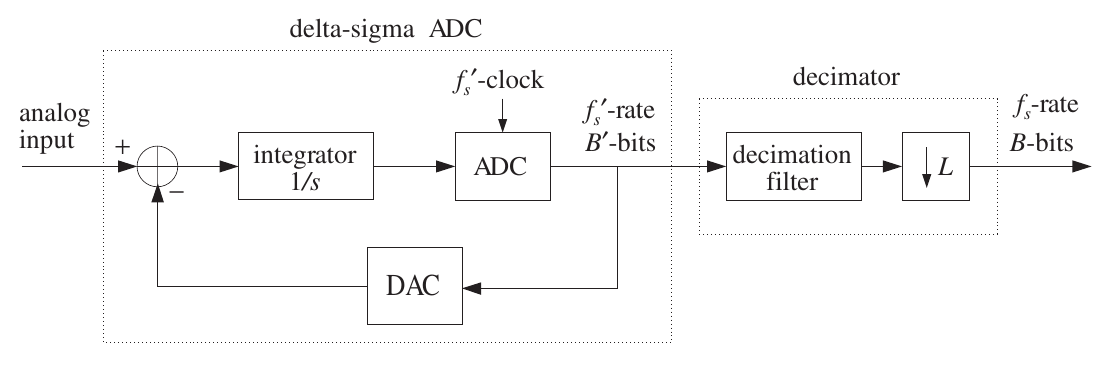
\includegraphics[width = 0.6\textwidth]{pic/deltaSigma.png}\centering
\newpage
\section{Digital-Analog-Wandler}
	\begin{minipage}{0.55\textwidth}
		Es gibt verschiedene Arten um Bitmuster in einen analogen Wert zu wandeln.
		\begin{itemize}
		 \item Unipolar Natural Binary
		 \item Bipolar Offset Binary
		 \item Bipolar Two's Complement
		\end{itemize}
	\end{minipage}\begin{minipage}{0.05\textwidth} $ $\end{minipage}
	\begin{minipage}{0.5\textwidth}
		\begin{tikzpicture}[>=latex', scale=1.5]
			\draw[line width=1](-0.5,-0.75)--(0.5,-0.75)--(0.5,0.75)--(-0.5,0.75)--cycle;
			\node at(0,0){\footnotesize DAC};
			\draw[line width=1,->](0.5,0)--node[above]{\footnotesize$x_Q$}node[below]{\footnotesize \parbox{1cm}{\centering analog\\ output}}(1.5,0);
			\draw[line width=1,->](-1.5,0.5)node[left]{\footnotesize $b_1$}--node[above]{\footnotesize MSB}(-0.5,0.5);
			\draw[line width=1,->](-1.5,0.25)node[left]{\footnotesize $b_2$}--node[above]{\footnotesize }(-0.5,0.25);
			\draw[line width=1,->](-1.5,0)node[left]{\footnotesize $b_3$}--node[above]{\footnotesize }(-0.5,-0);
			\node[rotate=90] at (-1,-0.25){\footnotesize $\cdots$};
			\draw[line width=1,->](-1.5,-0.5)node[left]{\footnotesize $b_B$}--node[below]{\footnotesize LSB}(-0.5,-0.5);
			\node[rotate=90] at (-2.1,-0){\footnotesize $B$ input bits};

			\draw[line width=1,fill](0,-0.75)--(-0,-1)circle(0.05)node[right=2pt]{\footnotesize R \tiny (Reference)};
		\end{tikzpicture} 
	\end{minipage}

	\begin{tabularx}{1.0025\textwidth}{|p{5.5cm}|p{5.5cm}|p{6cm}|}
	 \hline&&\\[-0.35cm]
		\textbf{Unipolar Natural Binary} & \textbf{Bipolar Offset Binary} & \textbf{Bipolar Two's Complement}\\[0.1cm]
	 \hline&&\\[-0.35cm]
		\begin{tikzpicture}[>=latex', scale=1.7]
			\draw[->][line width=0.75](0,-0.1)--(0,2.2)node[above]{\footnotesize$x_Q$};
			\draw[->][line width=0.75](-0.1,0)--(2,0)node[right]{\footnotesize$B$};
			\draw[line width=0.5](0/4,0.1)--(0/4,-0.1)node[below]{\tiny $000$};
			\draw[line width=0.5](0.1,0/4)--(-0.1,0/4)node[left]{\tiny $0$};

			\draw[line width=1,CadetRed,dashed](0,0)--(2,2);
			\foreach \i in {0,...,7}
			{
				\draw[line width=0.5, gray,dashed](0,\i/4)--(\i/4,\i/4);
				\draw[line width=0.5, gray,dashed](\i/4,0)--(\i/4,\i/4);
				\draw[line width=1,CadetRed,fill](\i/4,\i/4)circle(0.05);
			}

			\draw[line width=0.5](1/4,0.1)--(1/4,-0.1)node[below, yshift=-5pt]{\tiny $001$};
			\draw[line width=0.5](2/4,0.1)--(2/4,-0.1)node[below]{\tiny $010$};
			\draw[line width=0.5](3/4,0.1)--(3/4,-0.1)node[below, yshift=-5pt]{\tiny $011$};
			\draw[line width=0.5](4/4,0.1)--(4/4,-0.1)node[below]{\tiny $100$};
			\draw[line width=0.5](5/4,0.1)--(5/4,-0.1)node[below, yshift=-5pt]{\tiny $101$};
			\draw[line width=0.5](6/4,0.1)--(6/4,-0.1)node[below]{\tiny $110$};
			\draw[line width=0.5](7/4,0.1)--(7/4,-0.1)node[below, yshift=-5pt]{\tiny $111$};

			\draw[line width=0.5](0.1,8/4)--(-0.1,8/4)node[left]{\tiny $R$};
			\draw[line width=0.5](0.1,7/4)--(-0.1,7/4)node[left]{\tiny $7Q$};
			\draw[line width=0.5](0.1,6/4)--(-0.1,6/4)node[left]{\tiny $6Q$};
			\draw[line width=0.5](0.1,5/4)--(-0.1,5/4)node[left]{\tiny $5Q$};
			\draw[line width=0.5](0.1,4/4)--(-0.1,4/4)node[left]{\tiny $4Q$};
			\draw[line width=0.5](0.1,3/4)--(-0.1,3/4)node[left]{\tiny $3Q$};
			\draw[line width=0.5](0.1,2/4)--(-0.1,2/4)node[left]{\tiny $2Q$};
			\draw[line width=0.5](0.1,1/4)--(-0.1,1/4)node[left]{\tiny $Q$};
		\end{tikzpicture}&
		\begin{tikzpicture}[>=latex', scale=1.7]
			\draw[->][line width=0.75](0,-0.1)--(0,2.2)node[above]{\footnotesize$x_Q$};
			\draw[->][line width=0.75](-0.1,1)--(2,1)node[right]{\footnotesize$B$};

			\draw[line width=0.5](4/4,1.1)--(4/4,0.9)node[below]{\tiny $100$};
			\draw[line width=0.5](0.1,0/4)--(-0.1,0/4)node[left]{\tiny $-R/2$};

			\draw[line width=1,CadetRed,dashed](0,0)--(2,2);
			\foreach \i in {1,...,3,5,6,7}
			{
				\draw[line width=0.5, gray,dashed](0,\i/4)--(\i/4,\i/4);
			}
			\foreach \i in {1,...,7}
			{
				\draw[line width=0.5, gray,dashed](\i/4,1)--(\i/4,\i/4);
			}
			\foreach \i in {0,...,7}
			{
				\draw[line width=1,CadetRed,fill](\i/4,\i/4)circle(0.05);
			}

			\draw[line width=0.5](1/4,0.9)--(1/4,1.1)node[above, fill=white]{\tiny $001$};
			\draw[line width=0.5](3/4,0.9)--(3/4,1.1)node[above, fill=white]{\tiny $011$};
			\draw[line width=0.5](2/4,0.9)--(2/4,1.1)node[above,yshift=5pt]{\tiny $010$};
			\draw[line width=0.5](5/4,1.1)--(5/4,0.9)node[below, yshift=-5pt]{\tiny $101$};
			\draw[line width=0.5](6/4,1.1)--(6/4,0.9)node[below]{\tiny $110$};
			\draw[line width=0.5](7/4,1.1)--(7/4,0.9)node[below, yshift=-5pt]{\tiny $111$};

			\draw[line width=0.5](0.1,8/4)--(-0.1,8/4)node[left]{\tiny $R/2$};
			\draw[line width=0.5](0.1,7/4)--(-0.1,7/4)node[left]{\tiny $3Q$};
			\draw[line width=0.5](0.1,6/4)--(-0.1,6/4)node[left]{\tiny $2Q$};
			\draw[line width=0.5](0.1,5/4)--(-0.1,5/4)node[left]{\tiny $Q$};
			\draw[line width=0.5](0.1,4/4)--(-0.1,4/4)node[left]{\tiny $0$};
			\draw[line width=0.5](0.1,3/4)--(-0.1,3/4)node[left]{\tiny $-Q$};
			\draw[line width=0.5](0.1,2/4)--(-0.1,2/4)node[left]{\tiny $-2Q$};
			\draw[line width=0.5](0.1,1/4)--(-0.1,1/4)node[left]{\tiny $-3Q$};
		\end{tikzpicture}&
		\begin{tikzpicture}[>=latex', scale=1.7]
			\draw[->][line width=0.75](0,-1.2)--(0,1.2)node[above]{\footnotesize$x_Q$};
			\draw[->][line width=0.75](-0.1,0)--(2,0)node[right]{\footnotesize$B$};

			\draw[line width=0.5](0/4,0.1)--(0/4,-0.1)node[below]{\tiny $ $};
			\draw[line width=0.5](0.1,0/4)--(-0.1,0/4)node[left]{\tiny $0$};

			\draw[line width=1,CadetRed,dashed](0,0)--(1,1);
			\foreach \i in {0,...,3}
			{
				\draw[line width=0.5, gray,dashed](0,\i/4)--(\i/4,\i/4);
				\draw[line width=0.5, gray,dashed](\i/4,0)--(\i/4,\i/4);
				\draw[line width=1,CadetRed,fill](\i/4,\i/4)circle(0.05);
			}

			\draw[line width=1,CadetRed,dashed](1,-1)--(2,0);
			\foreach \i in {4,...,7}
			{
				\draw[line width=0.5, gray,dashed](0,-2+\i/4)--(\i/4,-2+\i/4);
				\draw[line width=0.5, gray,dashed](\i/4,0)--(\i/4,-2+\i/4);
				\draw[line width=1,CadetRed,fill](\i/4,-2+\i/4)circle(0.05);
			}

			\draw[line width=0.5](2/4,0.1)--(2/4,-0.1)node[below,fill=white]{\tiny $010$};
			\draw[line width=0.5](1/4,0.1)--(1/4,-0.1)node[below, yshift=-5pt]{\tiny $001$};
			\draw[line width=0.5](3/4,0.1)--(3/4,-0.1)node[below, yshift=-5pt]{\tiny $011$};
			\draw[line width=0.5](4/4,-0.1)--(4/4,0.1)node[above]{\tiny $100$};
			\draw[line width=0.5](5/4,-0.1)--(5/4,0.1)node[above, yshift=5pt]{\tiny $101$};
			\draw[line width=0.5](6/4,-0.1)--(6/4,0.1)node[above]{\tiny $110$};
			\draw[line width=0.5](7/4,-0.1)--(7/4,0.1)node[above, yshift=5pt]{\tiny $111$};

			\draw[line width=0.5](0.1,-4/4)--(-0.1,-4/4)node[left]{\tiny $R/2$};
			\draw[line width=0.5](0.1,-3/4)--(-0.1,-3/4)node[left]{\tiny $-3Q$};
			\draw[line width=0.5](0.1,-2/4)--(-0.1,-2/4)node[left]{\tiny $-2Q$};
			\draw[line width=0.5](0.1,-1/4)--(-0.1,-1/4)node[left]{\tiny $-Q$};
			\draw[line width=0.5](0.1,4/4)--(-0.1,4/4)node[left]{\tiny $R/2$};
			\draw[line width=0.5](0.1,3/4)--(-0.1,3/4)node[left]{\tiny $3Q$};
			\draw[line width=0.5](0.1,2/4)--(-0.1,2/4)node[left]{\tiny $2Q$};
			\draw[line width=0.5](0.1,1/4)--(-0.1,1/4)node[left]{\tiny $Q$};
		\end{tikzpicture}\\[0.1cm]
	 \hline&&\\[-0.35cm]
		\fcolorbox{CadetRed}{white}{$x_Q = R\,\mysum{n=1}{B}{b_n\,2^{-n}}$}&\fcolorbox{CadetRed}{white}{$x_Q = R\,\left(\mysum{n=1}{B}{b_n\,2^{-n}}-\dfrac{1}{2}\right)$}&\fcolorbox{CadetRed}{white}{$x_Q = R\, \left(\overline{b_1}\,2^{-1}+\mysum{n=2}{B}{b_n\,2^{-n}}-\dfrac{1}{2}\right)$}\\[0.5cm]
	 \hline&&\\[-0.35cm]
		\fcolorbox{CadetRed}{white}{$x_Q = Q\cdot m$}$\quad$\fcolorbox{CadetRed}{white}{$m = \mysum{n=1}{B}{b_n\,2^{B-n}}$} & \fcolorbox{CadetRed}{white}{$x_Q = Q\cdot m'$}$\quad$\fcolorbox{CadetRed}{white}{$m' = m - 2^{B-1}$} & \fcolorbox{CadetRed}{white}{$x_Q = Q\cdot m''$}$\quad$\newline\fcolorbox{CadetRed}{white}{$m'' = m + (($-$1)^{b_1}-1)\,2^{B-1}$} \\[0.5cm]
	 \hline&&\\[-0.35cm]
		$m = 0,1,2,...,2^{B}-1$ & $m' = $-$2^{B-1},...,$-$1,0,1,...,2^{B-1}-1$& $m'' = $-$2^{B-1},...,$-$1,0,1,...,2^{B-1}-1$\\[0.1cm]
	 \hline&&\\[-0.35cm]
		$x_{Qmin} = 0$ & $x_{Qmin} = -R/2 $ &$x_{Qmin} = -R/2$ \\[0.1cm]
	\hline&&\\[-0.35cm]
		$x_{Qmax} = R-Q$ & $x_{Qmax} = R/2-Q$ &$x_{Qmax} = R/2-Q$ \\[0.1cm]
	 \hline	 
	\end{tabularx}\\

\section{Analog-Digital-Wandler}
	\vspace*{-0.3cm}\begin{minipage}{0.32\textwidth}
		Ein Analog-Digital-Wandler quantisiert einen analogen Wert in ein digitales Bitmuster.\\
	\end{minipage}\begin{minipage}{0.05\textwidth}$ $\end{minipage}
	\begin{minipage}{0.4\textwidth}
		\begin{tikzpicture}[>=latex', scale=1.5]
			\draw[line width=1](-0.5,-0.75)--(0.5,-0.75)--(0.5,0.75)--(-0.5,0.75)--cycle;
			\node at(0,0){\footnotesize ADC};
			\draw[line width=1,->](-1.5,0)--node[above]{\footnotesize$x$}node[below]{\footnotesize \parbox{1cm}{\centering analog\\ input}}(-0.5,0);
			\draw[line width=1,->](0.5,0.5)--node[above]{\footnotesize MSB}(1.5,0.5)node[right]{\footnotesize $b_1$};
			\draw[line width=1,->](0.5,0.25)--node[above]{\footnotesize }(1.5,0.25)node[right]{\footnotesize $b_2$};
			\draw[line width=1,->](0.5,0)--node[above]{\footnotesize }(1.5,-0)node[right]{\footnotesize $b_3$};
			\node[rotate=90] at (1,-0.25){\footnotesize $\cdots$};
			\draw[line width=1,->](0.5,-0.5)--node[below]{\footnotesize LSB}(1.5,-0.5)node[right]{\footnotesize $b_B$};
			\node[rotate=90] at (2.1,-0){\footnotesize $B$ output bits};

			\draw[line width=1,fill](0,-0.75)--(-0,-1)circle(0.05)node[right=2pt]{\footnotesize R \tiny (Reference)};
		\end{tikzpicture}
	\end{minipage}

	\begin{minipage}[t]{0.66\textwidth}
		\textbf{Successive Approximation:}\\[0.2cm]
		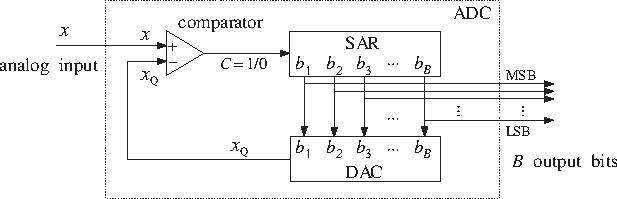
\includegraphics[width = 0.8\textwidth]{pic/sar.pdf}\\[0.2cm]
		Weil der SAR-AD-Wandler immer abrundet, muss vor dem Quantisieren zum Eingangswert eine halber Quantisierungsschritt dazugezählt werden\\[0.2cm]
		\fcolorbox{CadetRed}{white}{$y = x + \dfrac{1}{2}Q$}
	\end{minipage}
	\begin{minipage}[t]{0.3\textwidth}
		\begin{enumerate}
		\item Alle bits auf null setzen
		\item $b_1$ auf 1 setzen\\
			$x_Q>x\quad\rightarrow\quad b_1 = 0$\\
			$x_Q<x\quad\rightarrow\quad b_1 = 1$
		\item $b_2$ auf 1 setzen\\
			$x_Q>x\quad\rightarrow\quad b_2 = 0$\\
			$x_Q<x\quad\rightarrow\quad b_2 = 1$
		\item mit allen Bits wiederholen
		\item $b_B$ auf 1 setzen\\
			$x_Q>x\quad\rightarrow\quad b_B = 0$\\
			$x_Q<x\quad\rightarrow\quad b_B = 1$
		\end{enumerate}	
	\end{minipage}

\section{Dither}
	Dither ist ein kleines weisses Rauschen, dass vor dem Quantisieren zum Signal addiert wird.\\ Dies wird gemacht um:
	\begin{itemize}
	 \item Quantisierungsverzerrungen (Muster) zu eliminieren 
	 \item Das Quantisierungsrauschen weisser scheinen lassen
	\end{itemize}

	\begin{minipage}{0.55\textwidth}
		\textbf{Fehler:}\\[0.1cm]
		Da das Quantisierungsrauschen $e(n)$ und das Ditherrauschen $v(n)$ unkorreliert sind, wird der Fehler zwischen dem Eingangssignal und dem quanitsierten Signal zu:\\[0.2cm]
		\fcolorbox{CadetRed}{white}{$\varepsilon(n) = y_Q(n) - x(n) = v(n) + e(n)$}\\[0.2cm]
		\fcolorbox{CadetRed}{white}{$\sigma_\varepsilon^2 = \sigma_e^2 + \sigma_v^2 = \dfrac{Q^2}{12} + \sigma_v^2 $}
	\end{minipage}\begin{minipage}{0.05\textwidth}$ $\end{minipage}
	\begin{minipage}{0.4\textwidth}
		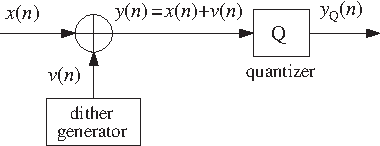
\includegraphics[width = 1\textwidth]{pic/ditherAdd.pdf}\\[0.2cm]
	\end{minipage}
	
	\subsection{Formen von Ditherrauschen}
		\begin{tabularx}{\textwidth}{|X|X|X|}
		 \hline
			\textbf{Gausssches Rauschen} & \textbf{Gleichverteiltes Rauschen} & \textbf{Dreieckverteiltes Rauschen}\\
		 \hline
			\begin{tikzpicture}[>=latex', scale=1.3]
				\def\si{0.5};
				\def\u{1.5};
				\draw[line width=0.75,->](-1.7,0)--(1.8,0)node[right]{\footnotesize$v$};
				\draw[line width=0.75,->](0,-0.1)--(0,1.9)node[right]{\footnotesize$p(v)$};
				\draw[smooth,samples=100,domain=-1.7:1.7, CadetRed, line width=1] plot (\x,{2/(sqrt(2*pi)*\si)*exp(-1/2*((\x)/\si)^2)});
				\draw[line width=0.75, black](0,0.1)--(0,-0.1) node [below] {\footnotesize$\mu=0$};
				\draw[line width=0.75, fill,white](0.3,0.95)--(0.6,0.95)--(0.6,1.1)--(0.3,1.1);

				\draw[line width=0.75, black,<->](0,0.85)--node [above, xshift=15pt , yshift=-2pt]{\footnotesize$\sigma_v = \frac{1}{2}Q$}(1.5-0.93,0.85);

				\draw[line width=0.75, black,<->](0,0.85)--node [above]{\footnotesize$ $}(1.5-2.07,0.85) ;
				\draw[line width=0.5](1.5,0.1)--(1.5,-0.1)node[below]{\footnotesize$\frac{3}{2} Q$};
				\draw[line width=0.5](-1.5,0.1)--(-1.5,-0.1)node[below]{\footnotesize$-\frac{3}{2} Q$};
			\end{tikzpicture}&
			\begin{tikzpicture}[>=latex', scale=1.3]
				\draw[->][line width=0.75](0,-0.3)--(0,1.2)node[right]{\footnotesize$p(v)$};
				\draw[->][line width=0.75](-1.7,0)--(1.8,0)node[below]{\footnotesize$v$};
				\draw[line width=1,CadetRed](-1.5,0)--(-1,0)--(-1,0.7)node[left]{\footnotesize$1/Q$}--(1,0.7)--(1,0)--(1.5,0);
				\draw[line width=0.5](-1,0.1)--(-1,-0.1)node[below]{\footnotesize -$Q/2$};
				\draw[line width=0.5](1,0.1)--(1,-0.1)node[below]{\footnotesize$Q/2$};
			\end{tikzpicture}&
			\begin{tikzpicture}[>=latex', scale=1.3]
				\draw[->][line width=0.75](0,-0.3)--(0,1.2)node[right]{\footnotesize$p(v)$};
				\draw[->][line width=0.75](-1.7,0)--(1.8,0)node[below]{\footnotesize$v$};
				\draw[line width=1,CadetRed](-1.7,0)--(-1.5,0)--(0,0.7)node[left, yshift=4pt]{\footnotesize$1/Q$}--(1.5,0)--(1.7,0);
				\draw[line width=0.5](-1.5,0.1)--(-1.5,-0.1)node[below]{\footnotesize -$Q$};
				\draw[line width=0.5](1.5,0.1)--(1.5,-0.1)node[below]{\footnotesize$Q$};
			\end{tikzpicture}\\
		 \hline&&\\[-0.3cm]
			$p(v) = \dfrac{\e^{-v^2/(2\,\sigma_v^2)}}{\sqrt{2\pi\sigma_v^2}}$&$p(v) = \begin{cases}\dfrac{1}{Q}, & -\frac{1}{2}Q\leq v\leq \frac{1}{2}Q\\0,& \text{sonst}\end{cases}$&$p(v) = \begin{cases}\dfrac{Q-|v|}{Q^2}, & -Q\leq v\leq Q\\0,& \text{sonst}\end{cases}$\\[0.65cm]
		 \hline&&\\[-0.3cm]
			$\sigma_v^2 = \frac{1}{4}Q^2$ & $\sigma_v^2 = \frac{1}{12}Q^2$&$\sigma_v^2 = \frac{1}{6}Q^2$\\[0.2cm]
		 \hline&&\\[-0.3cm]
			\fcolorbox{CadetRed}{white}{$\sigma_\varepsilon^2 = \frac{1}{12}Q^2 + \frac{1}{4}Q^2 = \frac{1}{3}Q^2$} &\fcolorbox{CadetRed}{white}{$\sigma_\varepsilon^2 = \frac{1}{12}Q^2 + \frac{1}{12}Q^2 = \frac{1}{6}Q^2$}&\fcolorbox{CadetRed}{white}{$\sigma_\varepsilon^2 = \frac{1}{12}Q^2 + \frac{1}{6}Q^2 = \frac{1}{4}Q^2$}\\[0.3cm]
		 \hline&&\\[-0.3cm]
			$4\times$ mehr Rauschen $(6\db)$ & $2\times$ mehr Rauschen $(3\db)$ & $3\times$ mehr Rauschen $(4.8\db)$\\[0.2cm]
		 \hline 
		\end{tabularx}\\

	\subsection{Subtractives Dither-Rauschen}
		\begin{minipage}{1\textwidth}
			Da das Dither-Rauschen selber erzeugt wurde kann es nach dem Quantisieren auch wieder abgezogen werden. Der Fehler reduziert sich dadurch wieder auf den Fehler des Quantisierungsrauschens.\\[0.2cm]
			\fcolorbox{CadetRed}{white}{$\varepsilon(n) = y_{out}(n)-x(n) = e(n)$}$\qquad$\fcolorbox{CadetRed}{white}{$\sigma_\varepsilon^2 = \frac{1}{12}Q^2$}
		\end{minipage}\\[0.5cm]
% 		\begin{minipage}{0.05\textwidth}$ $\end{minipage}
		\begin{minipage}{0.7\textwidth}
			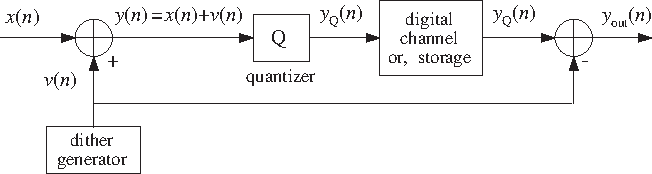
\includegraphics[width = \textwidth]{pic/ditherSub.pdf}\\[0.2cm]
		\end{minipage}





\chapter{Discrete-Time Systems \textcolor{black}{\small S.95}}
% 
% (c) Copyright 2016 Tabea Mendez
% 
% This source is free: you can redistribute it and/or modify
% it under the terms of the GNU General Public License as published by
% the Free Software Foundation, either version 3 of the License, or
% (at your option) any later version.
% 
% This source is distributed in the hope that it will be useful,
% but WITHOUT ANY WARRANTY; without even the implied warranty of
% MERCHANTABILITY or FITNESS FOR A PARTICULAR PURPOSE.  See the
% GNU General Public License for more details.
% 
% You should have received a copy of the GNU General Public License
% along with this source.  If not, see <http://www.gnu.org/licenses/>.
%
%%%%%%%%%%%%%%%%%%%%%%%%%%%%%%%%%%%%%%%%%%%%%%%%%%%%%%%%%%%%%%%%%%%%%%%%%%%%%%

	\begin{minipage}{0.6\textwidth}
		Ein Discrete-Time-System ist ein System, welches eine Eingangssequenz in eine Ausgangssequenz transformiert.\\
		Die Transformation kann dabei auf zwei Arten erfolgen:
		\begin{itemize}
		 \item Sample für Sample
		 \item Blockweise
		\end{itemize}
	\end{minipage}
	\begin{minipage}{0.4\textwidth}
		\begin{tikzpicture}[>=latex', scale=1.5]
			\draw[line width=1](-0.75,-0.5)--(0.75,-0.5)--(0.75,0.5)--node[above]{\footnotesize Discrete-Time-System}(-0.75,0.5)--cycle;
			\draw[line width=1,->](-1.8,0)--node[above]{\footnotesize$x(n)$}node[below]{\footnotesize\parbox{2cm}{\centering input Sequenz}}(-0.75,0);
			\draw[line width=1,<-](1.8,0)--node[above]{\footnotesize$y(n)$}node[below]{\footnotesize\parbox{2cm}{\centering output Sequenz}}(0.75,0);
			\node at (0,0){\huge$H$};
		\end{tikzpicture} 
	\end{minipage}\\

	\begin{minipage}{0.45\textwidth}
		\textbf{Sample für Sample}\\[0.2cm]
		$\begin{array}{c}
		\{x_0,x_1,x_2,...,x_n,...\}\\ \downarrow H\\
		\{y_0,y_1,y_2,...,y_n,...\}
		\end{array}$\\[0.2cm]
		\textbf{Bsp:}\\[0.1cm]
		$y(n) = 2\,x(n) + 3\,x(n-1) + 4\, x(n-2)$
	\end{minipage}
	\begin{minipage}{0.25\textwidth}
		\textbf{Blockweise}\\[0.2cm]
		$\begin{bmatrix}x_0\\x_1\\\vdots\\x_n\\\vdots\end{bmatrix}\xrightarrow H \begin{bmatrix}y_0\\y_1\\\vdots\\y_n\\\vdots\end{bmatrix}$\\[0.2cm]
	\end{minipage}
	\begin{minipage}{0.25\textwidth}
		\textbf{Bsp:}$\quad\vec y = H\cdot \vec x$\\[0.2cm]
		$\begin{bmatrix}y_0\\y_1\\y_2\\y_3\\y_4\end{bmatrix} =\begin{bmatrix}2 & 0 & 0\\3 & 2 & 0\\4 & 3 & 2\\0 & 4 & 3 \\0 & 0 & 4\end{bmatrix}\cdot \begin{bmatrix}x_0\\x_1\\x_2\end{bmatrix}$
	\end{minipage}
	
\section{Linearität und Zeitinvarianz}
	\textbf{Linearität:}\\[0.2cm]
		Für ein lineares System muss die Superpositionsbedingung erfüllt sein:\\[0.2cm]
		\fcolorbox{CadetRed}{white}{$y(n) = a_1\,H[x_1(n)]+ a_2\,H[x_2(n)]= H[a_1\,x_1(n) + a_2\,x_2(n)] $}\\[0.2cm]
	\begin{tikzpicture}[>=latex', scale=1.4]
		\def\s{0.3};
		\def\l{1};
		\def\r{0.15};
		\def\dis{0.8};

		\coordinate (h1) at (0,\dis);
		\draw[line width=1](h1)++(-\s,-\s)--++(2*\s,0)--++(0,2*\s)--++(-2*\s,0)--cycle node at(h1){$H$};
		\draw[line width=1,->](h1)++(-\l-\s,0)--node[above]{\footnotesize$x_1(n)$}++(\l,0);
		\draw[line width=1,->](h1)++(\s,0)--node[above]{\footnotesize$y_1(n)$}++(\l,0);
		\draw[line width=1](h1)++(\s+\l,0)node[right]{$a_1$}--++(0,\s)--++(2*\s,-\s)--++(-2*\s,-\s)--cycle;
		\draw[line width=1,->](h1)++(3*\s+\l,0)--++(\l/2,0)--++(0,-\dis+\r);

		\draw[line width=1,->](h1)++(3*\s+3/2*\l,-\dis)circle(\r)node{$+$};
		\draw[line width=1,->](h1)++(3*\s+3/2*\l+\r,-\dis)--node[above]{$y(n)$}++(\l,0);

		\coordinate (h2) at (0,-\dis);
		\draw[line width=1](h2)++(-\s,-\s)--++(2*\s,0)--++(0,2*\s)--++(-2*\s,0)--cycle node at(h2){$H$};
		\draw[line width=1,->](h2)++(-\l-\s,0)--node[above]{\footnotesize$x_2(n)$}++(\l,0);
		\draw[line width=1,->](h2)++(\s,0)--node[above]{\footnotesize$y_2(n)$}++(\l,0);
		\draw[line width=1](h2)++(\s+\l,0)node[right]{$a_2$}--++(0,\s)--++(2*\s,-\s)--++(-2*\s,-\s)--cycle;
		\draw[line width=1,->](h2)++(3*\s+\l,0)--++(\l/2,0)--++(0,\dis-\r);
	\end{tikzpicture}$\qquad\qquad$
	\begin{tikzpicture}[>=latex', scale=1.4]
		\def\s{0.3};
		\def\l{1};
		\def\r{0.15};
		\def\dis{0.8};

		\coordinate (h1) at (0,\dis);
		\draw[line width=1,->](h1)++(-\l-\s,0)--node[above]{\footnotesize$x_1(n)$}++(\l,0);
		\draw[line width=1](h1)++(-\s,0)node[right]{$a_1$}--++(0,\s)--++(2*\s,-\s)--++(-2*\s,-\s)--cycle;
		\draw[line width=1,->](h1)++(\s,0)--++(\l/2,0)--++(0,-\dis+\r);

		\draw[line width=1,->](h1)++(\s+1/2*\l,-\dis)circle(\r)node{$+$};
		\draw[line width=1,->](h1)++(\s+1/2*\l+\r,-\dis)--node[above]{$x(n)$}++(\l,0);

		\coordinate (h3) at (3/2*\l+\r+2*\s,0);
		\draw[line width=1](h3)++(-\s,-\s)--++(2*\s,0)--++(0,2*\s)--++(-2*\s,0)--cycle node at(h3){$H$};
		\draw[line width=1,->](h3)++(\s,0)--node[above]{\footnotesize$y(n)$}++(\l,0);

		\coordinate (h2) at (0,-\dis);
		\draw[line width=1,->](h2)++(-\l-\s,0)--node[above]{\footnotesize$x_2(n)$}++(\l,0);
		\draw[line width=1](h2)++(-\s,0)node[right]{$a_2$}--++(0,\s)--++(2*\s,-\s)--++(-2*\s,-\s)--cycle;
		\draw[line width=1,->](h2)++(\s,0)--++(\l/2,0)--++(0,\dis-\r);
	\end{tikzpicture}
	
	\textbf{Zeitinvarianz:}\\[0.2cm]
	Ein Zeitinvariantes System ändert seine Eigenschaften über die Zeit nicht.$\qquad$
	\fcolorbox{CadetRed}{white}{$y_D(n) = y(n-D)$}\\[0.2cm]
	\begin{tikzpicture}[>=latex', scale=1.4]
		\def\s{0.3};
		\def\l{1};
		\def\d{1};

		\coordinate (h3) at (0,0);
		\draw[line width=1,->](h3)++(-\l-\s,0)--node[above]{\footnotesize$x(n)$}++(\l,0);
		\draw[line width=1](h3)++(-\s,-\s)--++(2*\s,0)--++(0,2*\s)--++(-2*\s,0)--cycle node at(h3){$H$};
		\draw[line width=1,->](h3)++(\s,0)--node[above]{\footnotesize$y(n)$}++(\l,0);
		\draw[line width=1](h3)++(\s+\l,-\s)--++(2*\s,0)--++(0,2*\s)--++(-2*\s,0)--cycle node at(2*\s+\l,0){$D$};
		\draw[line width=1,->](h3)++(3*\s+\l,0)--node[above]{\footnotesize$y(n-D)$}++(\l,0);

		\coordinate (h4) at (0,-\d);
		\draw[line width=1,->](h4)++(-\l-\s,0)--node[above]{\footnotesize$x(n)$}++(\l,0);
		\draw[line width=1](h4)++(-\s,-\s)--++(2*\s,0)--++(0,2*\s)--++(-2*\s,0)--cycle node at(h4){$D$};
		\draw[line width=1,->](h4)++(\s,0)--node[above]{\footnotesize$x(n-D)$}node[below]{\footnotesize$x_D(n)$}++(\l,0);
		\draw[line width=1](h4)++(\s+\l,-\s)--++(2*\s,0)--++(0,2*\s)--++(-2*\s,0)--cycle node at(2*\s+\l,-\d){$H$};
		\draw[line width=1,->](h4)++(3*\s+\l,0)--node[above]{\footnotesize$y_D(n)$}++(\l,0);
	\end{tikzpicture}$\qquad\qquad$ 
	\begin{tikzpicture}[>=latex', scale=1.4]
		\def\s{0.4};
		\def\l{1};
		\def\d{0.4};

		\coordinate (h3) at (0,0);
		\draw[line width=1,->](h3)++(-\l-\s,0)--node[above]{$x(n)$}++(\l,0);

		\draw[line width=1](h3)++(-\s,-\s)--++(2*\s,0)--++(0,2*\s)--++(-2*\s,0)--cycle node at(h3){\parbox{2cm}{\centering  {\footnotesize Delay}\\ $D$}};
		\draw[line width=1,->](h3)++(\s,0)--node[above, xshift=6pt]{$x(n-D)$}++(\l,0);

		\coordinate (f1) at (-3,-\s);
		\draw[line width=0.5,->](f1)++(-0.1,0)--++(1.5*\l+0.2,0)node[right]{\footnotesize$n$};
		\draw[line width=0.5,->](f1)++(0,-0.1)node[below]{\tiny$0$}--++(0,\l)node[right]{\footnotesize$x(n)$};
		\foreach \i in {1,...,6}
		\draw[line width=0.5,fill](f1)++({(\i-1)/4},0)--++(0,{0.3*cos(\i*0.55*180/pi)+0.4})circle(0.03);

		\coordinate (f2) at (2.1,-\s);
		\draw[line width=0.5,->](f2)++(-0.1,0)--++(1.5*\l+\d+0.2,0)node[right]{\footnotesize$n$};
		\draw[line width=0.5,->](f2)++(0,-0.1)node[below]{\tiny$0$}--++(0,\l)node[right]{\footnotesize$x(n-D)$};
		\draw[line width=0.5,<->](f2)++(0,0.3)--node[above]{\tiny$D$}++(\d,0);

		\foreach \i in {1,...,6}
		\draw[line width=0.5,fill](f2)++({(\i-1)/4+\d},0)--++(0,{0.3*cos(\i*0.55*180/pi)+0.4})circle(0.03);
	\end{tikzpicture}\\[-0.3cm]

\section{Impulsantwort}
\vspace*{-0.6cm}\begin{minipage}{0.35\textwidth}
	Ein lineares, zeitinvariantes System, ist durch seine Impulsantwort vollständig bestimmt. Wird am Eingang ein Impuls $\delta(n)$ angelet, so antwortet das System mit der Impulsantwort $h(n)$.
\end{minipage}\begin{minipage}{0.05\textwidth}$ $\end{minipage}
	\begin{minipage}{0.65\textwidth}
			\begin{tikzpicture}[>=latex', scale=1.4]
			\def\s{0.4};
			\def\l{1};
			\def\d{0};

			\coordinate (h3) at (0,0);
			\draw[line width=1,->](h3)++(-\l-\s,0)--node[above]{$\delta(n)$}++(\l,0);

			\draw[line width=1](h3)++(-\s,-\s)--++(2*\s,0)--++(0,2*\s)--++(-2*\s,0)--cycle node at(h3){$H$};
			\draw[line width=1,->](h3)++(\s,0)--node[above]{$h(n)$}++(\l,0);

			\coordinate (f1) at (-2.3,-\s);
			\draw[line width=0.5,->](f1)++(-0.5,0)--++(1,0)node[right]{\footnotesize$n$};
			\draw[line width=0.5,->](f1)++(0,-0.1)node[below]{\tiny$0$}--++(0,\l)node[right]{\footnotesize$\delta(n)$};
			\foreach \i in {1}
			\draw[line width=1,fill](f1)++({(\i-1)/4},0)--++(0,{0.25*cos(\i*0.55*180/pi)+0.4})circle(0.04);

			\coordinate (f2) at (2.1,-\s);
			\draw[line width=0.5,->](f2)++(-0.5,0)--++(1.5*\l+\d+0.6,0)node[right]{\footnotesize$n$};
			\draw[line width=0.5,->](f2)++(0,-0.1)node[below]{\tiny$0$}--++(0,\l)node[right]{\footnotesize$h(n)$};
	% 		\draw[line width=0.5,<->](f2)++(0,0.3)--node[above]{\tiny$D$}++(\d,0);

			\foreach \i in {1,...,6}
			{
				\draw[line width=1,fill](f2)++({(\i-1)/4+\d},0)--++(0,{0.3*cos(\i*0.55*180/pi)+0.4})circle(0.04);
			}
		\end{tikzpicture} 

		\begin{tikzpicture}[>=latex', scale=1.4]
			\def\s{0.4};
			\def\l{1};
			\def\d{0.6};

			\coordinate (h3) at (0,0);
			\draw[line width=1,->](h3)++(-\l-\s,0)--node[above,, xshift=-5pt]{$\delta(n-k)$}++(\l,0);

			\draw[line width=1](h3)++(-\s,-\s)--++(2*\s,0)--++(0,2*\s)--++(-2*\s,0)--cycle node at(h3){$H$};
			\draw[line width=1,->](h3)++(\s,0)--node[above, xshift=5pt]{$h(n-k)$}++(\l,0);

			\coordinate (f1) at (-2.3,-\s);
			\draw[line width=0.5,->](f1)++(-0.5,0)--++(1,0)node[right]{\footnotesize$n$};
			\draw[line width=0.5,->](f1)++(-0.4,-0.1)node[below]{\tiny$0$}--++(0,\l)node[right]{\footnotesize$\delta(n-k)$};
			\foreach \i in {1}
			{
			\draw[line width=1,fill](f1)++({(\i-1)/4+0.2},0)node[below]{$k$}--++(0,{0.25*cos(\i*0.55*180/pi)+0.4})circle(0.04);
			}
			\coordinate (f2) at (2.1,-\s);
			\draw[line width=0.5,->](f2)++(-0.5,0)--++(1.5*\l+\d+0.6,0)node[right]{\footnotesize$n$};
			\draw[line width=0.5,->](f2)++(0,-0.1)node[below]{\tiny$0$}--++(0,\l)node[right]{\footnotesize$h(n-k)$};
	% 		\draw[line width=0.5,<->](f2)++(0,0.3)--node[above]{\tiny$D$}++(\d,0);

			\foreach \i in {1}
			{
				\draw[line width=1,fill](f2)++({(\i-1)/4+\d},0)node[below]{$k$}--++(0,{0.3*cos(\i*0.55*180/pi)+0.4})circle(0.04);
			}
			\foreach \i in {2,...,6}
			{
				\draw[line width=1,fill](f2)++({(\i-1)/4+\d},0)node[below]{$ $}--++(0,{0.3*cos(\i*0.55*180/pi)+0.4})circle(0.04);
			}
		\end{tikzpicture}
	\end{minipage}\\[-0.2cm]
	\begin{description}
		\item [LTI-Form:] $ $\\
		\begin{minipage}[t]{0.65\textwidth}
		Eingangssequenz ist Folge von gewichteten und verzögerten Diracs.\\
		Ausgangssequenz ist Überlagerung der gewichteten und verzögerten Impulsantworten.
		\end{minipage}\begin{minipage}[t]{0.03\textwidth}$ $\end{minipage}
		\begin{minipage}[t]{0.28\textwidth}
		$ $\\[-0.35cm]\fcolorbox{CadetRed}{white}{$y(n) = \mysum{m}{}{x(m)\cdot h(n-m)}$}\\
		\end{minipage}
		\item [Direkt Form:]$ $\\
		\begin{minipage}{\textwidth}
		Faltung der Eingangssequenz mit der Impulsantwort$\qquad\qquad\qquad\qquad\quad\;\,$
		\fcolorbox{CadetRed}{white}{$y(n) = \mysum{m}{}{h(m)\cdot x(n-m)}$}
		\end{minipage}
	\end{description}

\section{FIR und IIR Filter}
	Diskrete LTI-Systeme werden über ihre Impulsantwort klassifiziert\\[0.2cm]
	\begin{minipage}{0.45\textwidth}
		\begin{itemize}
		\item \textbf{FIR Filter:} Finite Impulse Response\\[-0.2cm]
		\item \textbf{IIR Filter:} Infinite Impulse Response\\[0.4cm]
		\end{itemize}
	\end{minipage}
	\begin{minipage}{0.5\textwidth}
		\begin{tikzpicture}[>=latex', scale=1.6]
			\def\s{0.4};
			\def\l{1};
			\def\d{0};

			\coordinate (f2) at (0,0);
			\draw[line width=0.5,->](f2)++(-0.4,0)--++(2.1*\l+\d+0.6,0)node[right]{\footnotesize$n$};
			\draw[line width=0.5,->](f2)++(0,-0.1)node[below]{\footnotesize$0$}--++(0,\l)node[right]{\footnotesize FIR $h(n)$};
	% 		\draw[line width=0.5,<->](f2)++(0,0.3)--node[above]{\tiny$D$}++(\d,0);

			\foreach \i in {1,...,5}
			{
				\draw[line width=1,fill](f2)++({(\i-1)/4+\d},0)--++(0,{0.3*cos(\i*0.55*180/pi)+0.4})circle(0.04);
			}
			\foreach \i in {6}
			{
				\draw[line width=1,fill](f2)++({(\i-1)/4+\d},0)node[below]{\footnotesize$M$}--++(0,{0.3*cos(\i*0.55*180/pi)+0.4})circle(0.04);
			}
			\foreach \i in {0,7,8,9}
			{
				\draw[line width=1,fill](f2)++({(\i-1)/4+\d},0)--++(0,{0})circle(0.04);
			}

			\coordinate (f2) at (3.5,0);
			\draw[line width=0.5,->](f2)++(-0.4,0)--++(2.1*\l+\d+0.6,0)node[right]{\footnotesize$n$};
			\draw[line width=0.5,->](f2)++(0,-0.1)node[below]{\footnotesize$0$}--++(0,\l)node[right]{\footnotesize IIR $h(n)$};
	% 		\draw[line width=0.5,<->](f2)++(0,0.3)--node[above]{\tiny$D$}++(\d,0);

			\foreach \i in {1,...,6}
			{
				\draw[line width=1,fill](f2)++({(\i-1)/4+\d},0)--++(0,{0.3*cos(\i*0.55*180/pi)+0.4})circle(0.04);
			}
			\foreach \i in {0}
			{
				\draw[line width=1,fill](f2)++({(\i-1)/4+\d},0)--++(0,{0})circle(0.04);
			}
			\foreach \i in {8,9,10}
			{
				\draw[line width=1,fill](f2)++({(\i-1)/4.65+\d},0)++(0,{0.1})circle(0.015);
			}
		\end{tikzpicture} 
	\end{minipage}\\[-0.6cm]
	
	\begin{description}
	 \item [FIR Filter:]$ $\\[0.1cm]
		Ein FIR Filter hat eine endliche Anzahl Koeffizienten, die nicht Null sind.\\[0.1cm]
		\begin{tabular}{ll}
		 Filterkoeffizienten & \fcolorbox{CadetRed}{white}{$\{h_0,h_1,h_2,...,h_M,0,0,0,...\}$}\\[0.2cm]
		 Ordung: & \fcolorbox{CadetRed}{white}{$M$}\\[0.1cm]
		 Filterlänge: & \fcolorbox{CadetRed}{white}{$L_h = M + 1$}\\
		\end{tabular}\\[0.2cm]
		Für FIR Filter vereinfacht sich die Direkte Faltungsform zu:\\[0.1cm]
		$y(n) = h_0\, x(n) + h_1\, x(n-1) + h_2\, x(n-2) + ...  + h_M\, x(n-M)$\\[0.2cm]
		\fcolorbox{CadetRed}{white}{$y(n) = \mysum{m=0}{M}{h(m)\cdot x(n-m)}$}\\[0.1cm]
	 \item [IIR Filter:]$ $\\[0.1cm]
		Ein IIR Filter hat eine unendliche Anzahl Koeffizienten, die nicht Null sind. Da solche Filter nicht realisiert werden können, wird er Fokus auf eine wichtige Unterklasse der IIR Filter gelegt:\\ \textbf{IIR Filter die den Ausgang zurückführen (Feedback-Loop) }\\[0.1cm]
		Die Impulsantwort solcher IIR Filter kann in folgender Form geschrieben werden:\\[0.2cm]
		\fcolorbox{CadetRed}{white}{$h(n) = \underbrace{\mysum{i=1}{M}{a_i\,h(n-i)}}_{\text{IIR-Teil}}+ \underbrace{\mysum{j=0}{L}{b_j\,\delta(n-j)}}_{\text{FIR-Teil}}$}\\[0.2cm]
		und die Ein-Ausgangsgleichung folgendermassen:\\[0.1cm]
		$y(n) = \underbrace{a_1\,y(n-1) + a_2\,y(n-2) + ... + a_M\,y(n-M)}_{\text{IIR-Teil}} + \underbrace{b_0\, x(n) + b_1\, x(n-1) + b_2\, x(n-2) + ...  + b_L\, x(n-L)}_{\text{FIR-Teil}}$\\[0.2cm]
		\fcolorbox{CadetRed}{white}{$y(n) = \underbrace{\mysum{i=1}{M}{a_i\,y(n-i)}}_{\text{IIR-Teil}}+ \underbrace{\mysum{j=0}{L}{b_j\,x(n-j)}}_{\text{FIR-Teil}}$}\\[0.2cm]
	\end{description}
		
\section{Kausalität und Stabilität}
	\textbf{Kausalität}\\[0.2cm]
	Es gibt drei Arten von Signalen und demzufolge auch drei Arten von LTI-Systemen.\\[-0.65cm]
	\begin{itemize}
	 \item Kausale Signale / LTI-Systeme\\[-0.65cm]
	 \item Antikausale Signale / LTI-Systeme\\[-0.65cm]
	 \item Gemischte Signale / LTI-Systeme
	\end{itemize}

	\begin{tabularx}{\textwidth}{|X|X|X|}
	 \hline&&\\[-0.4cm]
		\textbf{Kausal} & \textbf{Antikausal} & \textbf{Gemischt}\\
	 \hline
		\begin{tikzpicture}[>=latex', scale=1.4]
			\def\s{0.4};
			\def\l{1};
			\def\d{0};

			\coordinate (f2) at (0,0);
			\draw[line width=0.5,->](f2)++(-1.5,0)--++(3.1,0)node[right]{\footnotesize$n$};
			\draw[line width=0.5,->](f2)++(0,-0.1)node[below]{\footnotesize$0$}--++(0,\l+0.1)node[right]{\footnotesize $x(n)$};
			\foreach \i in {1,...,6}
			{
				\draw[line width=1,fill](f2)++({(\i-1)/4+\d},0)--++(0,{0.3*cos(\i*0.55*180/pi)+0.4})circle(0.04);
			}
			\foreach \i in {-4,...,0}
			{
				\draw[line width=1,fill](f2)++({(\i-1)/4+\d},0)--++(0,{0})circle(0.04);
			}
		\end{tikzpicture}&		
		\begin{tikzpicture}[>=latex', scale=1.4]
			\def\s{0.4};
			\def\l{1};
			\def\d{0};
			
			\coordinate (f2) at (4,0);
			\draw[line width=0.5,->](f2)++(-1.5,0)--++(3.1,0)node[right]{\footnotesize$n$};
			\draw[line width=0.5,->](f2)++(0,-0.1)node[below]{\footnotesize$0$}--++(0,\l+0.1)node[right]{\footnotesize $x(n)$};

			\foreach \i in {-4,...,0}
			{
				\draw[line width=1,fill](f2)++({(\i-1)/4+\d},0)--++(0,{0.3*cos(\i*0.55*180/pi)+0.4})circle(0.04);
			}
			\foreach \i in {1,...,6}
			{
				\draw[line width=1,fill](f2)++({(\i-1)/4+\d},0)--++(0,{0})circle(0.04);
			}

		\end{tikzpicture}&		
		\begin{tikzpicture}[>=latex', scale=1.4]
			\def\s{0.4};
			\def\l{1};
			\def\d{0};

			\coordinate (f2) at (8,0);
			\draw[line width=0.5,->](f2)++(-1.5,0)--++(3.1,0)node[right]{\footnotesize$n$};
			\draw[line width=0.5,->](f2)++(0,-0.1)node[below]{\footnotesize$0$}--++(0,\l+0.1)node[right]{\footnotesize $x(n)$};

			\foreach \i in {-4,...,6}
			{
				\draw[line width=1,fill](f2)++({(\i-1)/4+\d},0)--++(0,{0.3*cos(\i*0.55*180/pi)+0.4})circle(0.04);
			}
		\end{tikzpicture}\\
	 \hline&&\\[-0.35cm]
		ungleich Null für $n>=0$ & ungleich Null für $n<=-1$  & ungleich Null alle $n$\\[0.05cm]
	 \hline
	\end{tabularx}
	
	\textbf{Stabilität:}\\[0.2cm]
	Ein LTI-System ist stabil, wenn ein begrenzter Eingang nur einen begrenzten Ausgang generiert.\\[0.2cm]
	\fcolorbox{CadetRed}{white}{$\mysum{n=-\infty}{\infty}{|h(n)|}<\infty$}\\
	
	\textbf{Stabilität und Kausalität:}
	\begin{itemize}
	 \item Stabilität und Kausalität sind unabhänging voneinander
	 \item Stabilität ist zwingend Kausalität nicht
	 \item Um ein stabiles, antikausales oder gemischtes LTI-System zu realisieren, wird der Ausgang und die Anzahl Samples verzögert, die in der Zukunft liegen würden.\\
	 Geht die Impulsantwort bis ins unendliche in die Zukunft, so wird diese einfach abgeschnitten, wenn die Koeffizienten genug klein geworden sind $\rightarrow$ Approximation
	\end{itemize}

	

	




\chapter{FIR Filter und Faltung \textcolor{black}{\small S.121}}
% 
% (c) Copyright 2016 Tabea Mendez
% 
% This source is free: you can redistribute it and/or modify
% it under the terms of the GNU General Public License as published by
% the Free Software Foundation, either version 3 of the License, or
% (at your option) any later version.
% 
% This source is distributed in the hope that it will be useful,
% but WITHOUT ANY WARRANTY; without even the implied warranty of
% MERCHANTABILITY or FITNESS FOR A PARTICULAR PURPOSE.  See the
% GNU General Public License for more details.
% 
% You should have received a copy of the GNU General Public License
% along with this source.  If not, see <http://www.gnu.org/licenses/>.
%
%%%%%%%%%%%%%%%%%%%%%%%%%%%%%%%%%%%%%%%%%%%%%%%%%%%%%%%%%%%%%%%%%%%%%%%%%%%%%%

\section{Blockverarbeitungsmethoden}
	\begin{minipage}{0.65\textwidth}
		Oft werden analoge Signale eine bestimmte Zeit lang abgetastet und in einem Vektor gespeichert. Dieser wird dann als Block verarbeitet.\\[0.2cm]
		\textbf{Messdauer:}$\qquad\qquad\;\;$\fcolorbox{CadetRed}{white}{$T_{Lx} = L_x\cdot T$}\\[0.2cm]
		\textbf{Anzahl Samples:}$\qquad$\fcolorbox{CadetRed}{white}{$L_x = T_{Lx}\cdot f_s$}
	\end{minipage}\begin{minipage}{0.05\textwidth}$ $\end{minipage}
	\begin{minipage}{0.3\textwidth}
		\begin{tikzpicture}[>=latex', scale=1.4]
			\def\s{0.4};
			\def\l{1};
			\def\d{0};

			\coordinate (f2) at (0,0);
			\draw[line width=0.5,->](f2)++(-1.5,0)--++(3.1,0)node[right]{\footnotesize$n$};
			\draw[line width=0.5,->](f2)++({(-3-1)/4+\d},-0.1)node[below]{\footnotesize$0$}--++(0,\l+0.1)node[right]{\footnotesize $x(n)$};
			\foreach \i in {-3,...,4}
			{
				\draw[line width=1,fill](f2)++({(\i-1)/4+\d},0)--++(0,{0.3*cos(\i*0.55*180/pi)+0.4})circle(0.04);
			}
			\draw[line width=1,fill](f2)++({(5-1)/4+\d},0)node[below]{\footnotesize$L_x$-$1$}--++(0,{0.3*cos(5*0.55*180/pi)+0.4})circle(0.04);

			\draw[line width=0.5,fill](f2)++({(6-1)/4+\d},0.1)--++(0,{-0.2});

			\draw[line width=0.5, black](f2)++({-(5-1)/4+\d},-0.4)--++(0,-0.2);
			\draw[line width=0.5, black,<->](f2)++({-(5-1)/4+\d},-0.5)--node[above]{\footnotesize$T_{Lx}$}++({2*(5.5-1)/4+\d},0);
			\draw[line width=0.5, black](f2)++({-(5-1)/4+\d},-0.5)++({2*(5.5-1)/4+\d},0)--++(0,0.1)--++(0,-0.2)--++(0,0.1);

			\coordinate (f2) at (0,0.8);
			\draw[line width=0.5](f2)++({(3-1)/4+\d},0.1)--node[fill=white]{\footnotesize$T$}++(-0.25,0);
			\draw[line width=0.5, black](f2)++({(2-1)/4+\d},0)--++(0,0.2);
			\draw[line width=0.5, black](f2)++({(3-1)/4+\d},0)--++(0,0.2);
			\draw[line width=0.5, black,<-](f2)++({(2-1)/4+\d},0.1)--++(-0.25,0);
			\draw[line width=0.5, black,<-](f2)++({(3-1)/4+\d},0.1)--++(0.25,0);
		\end{tikzpicture} 
	\end{minipage}

	\subsection{Blocklängen und Grenzen der Faltungssumme}
		\begin{minipage}{0.45\textwidth}
			Gegeben:\\[-0.3cm]
			\begin{itemize}
			 \item Eingangsvektor $x$ der Länge $L_x$\\[-0.3cm]
			 \item Kausales FIR-Filter $h$ der Ordung $M$ und Länge $L_h$\\[0.1cm]
			 \fcolorbox{CadetRed}{white}{$L_h = M + 1$}\\[-0.3cm]
			 \item Ausgangsvektor der Länge $L_y$\\[0.1cm]
			 \fcolorbox{CadetRed}{white}{$L_y = L_x + L_h -1 = L_x + M $}\\[-0.3cm]
			\end{itemize}$ $\\[0.1cm]
		\end{minipage}
		\begin{minipage}{0.03\textwidth}$ $\end{minipage}
		\begin{minipage}{0.5\textwidth}
			\begin{tikzpicture}[>=latex', scale=1.4]
				\def\b{0.45};
				\def\lx{3};
				\def\m{2.2};

				\coordinate (h) at (0,0);
				\coordinate (x) at (0,-1.1);
				\coordinate (y) at (0,-2.2);

				\draw[line width=0.5,->](h)node[left]{$h = $}++(0,-\b/2)--node[above]{ $ h_0,h_1,h_2,...,h_M$}++(\m,0)--++(0,\b)--++(-\m,0)--cycle;
				\draw[decorate,decoration={brace,amplitude=5pt}](h)++(\m,-\b/2-0.05) --node[below=3pt]{ $M+1$} ++(-\m,0) ;

				\draw[line width=0.5,->](x)node[left]{$x = $}++(0,-\b/2)--node[above]{ $ x_0,x_1,x_2,x_3,...,x_{L_x-1}$}++(\lx,0)--++(0,\b)--++(-\lx,0)--cycle;
				\draw[decorate,decoration={brace,amplitude=5pt}](x)++(\lx,-\b/2-0.05) --node[below=3pt]{ $L_x$} ++(-\lx,0) ;

				\draw[line width=0.5,->](y)node[left]{$y = h \ast x= $}++(0,-\b/2)--node[above]{ $ y_0,y_1,y_2,...,y_{L_x-1}$}++(\lx,0)--++(0,\b)--++(-\lx,0)--cycle;
				\draw[line width=0.5,->](y)++(\lx,-\b/2)--node[above]{ $  y_{L_x},...,y_{L_x+M}  $}++(\m,0)--++(0,\b)--++(-\m,0)--cycle;
				\draw[decorate,decoration={brace,amplitude=5pt}](y)++(\lx+\m,-\b/2-0.05) --node[below=3pt]{ $M$} ++(-\m,0) ;
				\draw[decorate,decoration={brace,amplitude=5pt}](y)++(\lx,-\b/2-0.05) --node[below=3pt]{ $L_x$} ++(-\lx,0) ;
				\draw[decorate,decoration={brace,amplitude=5pt}](y)++(\lx+\m,-\b/2-0.55) --node[below=3pt]{ $L_y$} ++(-\lx-\m,0) ;
			\end{tikzpicture} 
		\end{minipage}\\[-0.5cm]
		\textbf{Grenzen der Faltungssumme}\\[0.2cm]
		Für jedes $y(n)$ müssen die Grenzen der Summe festgelegt werden. Dabei müssen folgende zwei Bedinungen eingehalten werden:\\[0.2cm]
		$(0\leq m\leq L_x-1\quad\cap\quad0\leq n-m\leq M )\qquad\cup\qquad (0\leq m\leq M \quad\cap\quad 0\leq n-m\leq L_x-1)$ \\[0.2cm]
		\textbf{Berechnung des Ausgangsvektors \bm{$y(n)$}:}\\[0.4cm]
		LTI-Form:$\qquad\;\;\;\;$\fcolorbox{CadetRed}{white}{$y(n) = \mysum{m = max\{0,n-M\}}{min\{n,L_x-1\}}{x(m)\cdot h(n-m)}$}$\qquad\,$ für$\quad n = 0,1,2,...,L_x+M-1$\\[0.4cm]
		Direct-Form:$\qquad$\fcolorbox{CadetRed}{white}{$y(n) = \mysum{m = max\{0,n-L_x+1\}}{min\{n,M\}}{h(m)\cdot x(n-m)}$}$\quad$ für$\quad n = 0,1,2,...,L_x+M-1$\\[0.2cm]
		

	\subsection{Transienten und Steady-State}\label{Transienten und Steady-State}
		\vspace*{-0.9cm}\begin{minipage}{0.4\textwidth}
			Bei der Faltung zwischen dem Eingang $x(n)$ und der Impulsantwort $h(n)$ gibt es drei Phasen:\\[-0.3cm]
			\begin{itemize}
			\item Input-On Transiente
			\item Steady State
			\item Input-Off Transiente
			\end{itemize}
		\end{minipage}\begin{minipage}{0.03\textwidth}$ $\end{minipage}
		\begin{minipage}{0.5\textwidth}
			\begin{tikzpicture}[>=latex', scale=1.3]
				\def\b{0.35};
				\def\lx{0.4};
				\def\m{0.7};

				\coordinate (f2) at (0,0);
				\draw[line width=0.5,->](-0.3,0)--(7.5,0)node[right]{\footnotesize$n$};
				\draw[line width=0.5,->](0,-0.2)node[below]{\footnotesize$0$}--(0,2)node[right]{\footnotesize $y(n)$};
				\foreach \i in {0,...,4}
				{
					\draw[line width=1,fill,CadetRed](\i/3.5,0)--(\i/3.5,{0.2*\i+0.6})circle(0.04);
				}
				\def\i{5};
				\draw[line width=1,fill,greenT](\i/3.5,0)--(\i/3.5,{0.2*\i+0.6})circle(0.04);
				\draw[line width=0.5,fill](\i/3.5,0.1)--(\i/3.5,-0.1)node[below]{M};
				\foreach \i in {6,...,18}
				{
					\draw[line width=1,fill,greenT](\i/3.5,0)--(\i/3.5,{0.2*5+0.6})circle(0.04);
				}
				\def\i{19};
				\draw[line width=1,fill,greenT](\i/3.5,0)--(\i/3.5,{0.2*5+0.6})circle(0.04);
				\draw[line width=0.5,fill](\i/3.5,0.1)--(\i/3.5,-0.1)node[below]{$L_x\text{\tiny$^-$}1$};
				\foreach \i in {20,...,23}
				{
					\draw[line width=1,fill,blueT](\i/3.5,0)--(\i/3.5,{-0.2*\i+0.2*24+0.6})circle(0.04);
				}
				\def\i{24};
				\draw[line width=1,fill,blueT](\i/3.5,0)--(\i/3.5,{-0.2*\i+0.2*24+0.6})circle(0.04);
				\draw[line width=0.5,fill](\i/3.5,0.1)--(\i/3.5,-0.1)node[below]{$L_x\text{\tiny$^-$}1\text{\tiny$^+$}M$};

				\coordinate (f2) at (0,-0.8);
				\draw[line width=0.75,<->](f2)--node[fill=white]{\parbox{1.25cm}{\footnotesize\centering input-on}}++(5/3.5,0);
				\draw[line width=0.75, black](f2)++(0,0.2)--++(0,-0.4);
				\draw[line width=0.75, black](f2)++(5/3.5,0.2)--++(0,-0.4);

				\draw[line width=1,->,CadetRed](f2)++(0.4,-0.55)++(0,-\b/2)--node[above]{\footnotesize$x$}++(\m,0)--++(0,\b)--++(-\m,0)--cycle;
				\draw[line width=1,->,CadetRed](f2)++(0.4,-0.55)++(-0.2,-\b*3/2)--node[above]{\footnotesize$h$}++(\lx,0)--++(0,\b)--++(-\lx,0)--cycle;

				\coordinate (f2) at (5/3.5,-0.8);
				\draw[line width=0.75,<->](f2)--node[fill=white]{\parbox{1.7cm}{\footnotesize\centering steady state}}++(14/3.5,0);
				\draw[line width=0.75, black](f2)++(0,0.2)--++(0,-0.4);
				\draw[line width=0.75, black](f2)++(14/3.5,0.2)--++(0,-0.4);

				\draw[line width=1,->,greenT](f2)++(1.7,-0.55)++(0,-\b/2)--node[above]{\footnotesize$x$}++(\m,0)--++(0,\b)--++(-\m,0)--cycle;
				\draw[line width=1,->,greenT](f2)++(1.7,-0.55)++(0.15,-\b*3/2)--node[above]{\footnotesize$h$}++(\lx,0)--++(0,\b)--++(-\lx,0)--cycle;

				\coordinate (f2) at (19/3.5,-0.8);
				\draw[line width=0.75,<->](f2)--node[fill=white]{\parbox{1.25cm}{\footnotesize\centering input-off}}++(5/3.5,0);
				\draw[line width=0.75, black](f2)++(0,0.2)--++(0,-0.4);
				\draw[line width=0.75, black](f2)++(5/3.5,0.2)--++(0,-0.4);

				\draw[line width=1,->,blueT](f2)++(0.4,-0.55)++(0,-\b/2)--node[above]{\footnotesize$x$}++(\m,0)--++(0,\b)--++(-\m,0)--cycle;
				\draw[line width=1,->,blueT](f2)++(0.4,-0.55)++(0.5,-\b*3/2)--node[above]{\footnotesize$h$}++(\lx,0)--++(0,\b)--++(-\lx,0)--cycle;
			\end{tikzpicture} 
		\end{minipage}\\[0.5cm]
		\begin{minipage}{1\textwidth}
			\fcolorbox{CadetRed}{white}{$y(n) = \left\{\begin{array}{ccrclcl}
			\mysum{m = 0}{n}{h(m)\cdot x(n-m)}&&0\;\leq\;& n& < \;M &&\text{Input-On Transiente}\\
			\mysum{m = 0}{M}{h(m)\cdot x(n-m)}&& M\;\leq\;& n& \leq\; L_x-1 &&\text{Steady State}\\
			\mysum{m = n-L_x+1}{M}{h(m)\cdot x(n-m)}&& L_x-1\;< \;& n&\leq\; L_x-1+M &&\text{Input-Off Transiente}
			\end{array}\right.$}
		\end{minipage}
\newpage		
	\subsection{Faltungstabelle (Convolution table)}
		\begin{minipage}{0.57\textwidth}
			Die Faltung kann in Form einer Tabelle geschrieben werden.\\[0.2cm]
			Für den $n$-ten Wert der Ausgangssequenz $y(n)$ müssen die Werte der entsprechenden Diagonale zusammengezählt werden.\\[0.2cm]
			\fcolorbox{CadetRed}{white}{$y(n) = \mysum{i,j\atop i+j=n}{}{h(i)\cdot x(j)}$}\\[0.4cm]
			Bsp: $\quad y(5) = \mysum{i,j\atop i+j=5}{}{h(i)\cdot x(j)} = h(3)\,x(2) + h(2)\,x(3) + h(1)\,x(4)$
		\end{minipage}
		\begin{minipage}{0.01\textwidth}$ $\end{minipage}
		\begin{minipage}{0.4\textwidth}
		 	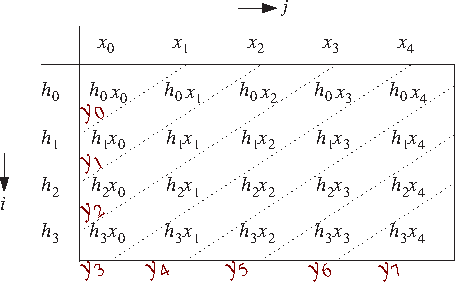
\includegraphics[width = 1\textwidth]{pic/convTab.pdf}
		\end{minipage}


	\subsection{LTI-Form Faltung }
		\begin{minipage}{0.37\textwidth}
		 	Der Eingangsvektor $x(n)$ kann in gewichtete und verzögerte Diracs aufgesplittet werden. Diese werden einzeln durch das LTI-System geschickt und deren gewichteten und verzögerten Impulsantworten summiert.
		 \end{minipage}\begin{minipage}{0.03\textwidth}$ $\end{minipage}
		 \begin{minipage}{0.62\textwidth}
		 	$\begin{array}{lcl}
		 	  x& = &x_0\,[\,1,\,0,\,0,\,0,\,0\,]\\
		 	   & + &x_1\,[\,0,\,1,\,0,\,0,\,0\,]\\
		 	   & + &x_2\,[\,0,\,0,\,1,\,0,\,0\,]\\
		 	   & + &x_3\,[\,0,\,0,\,0,\,1,\,0\,]\\
		 	   & + &x_4\,[\,0,\,0,\,0,\,0,\,1\,]\\
		 	 \end{array}\xrightarrow {\;\;\;H\;\;\;}
		 	 \begin{array}{lcl}
		 	  y& = &x_0\,[\,h_0,\,h_1,\,h_2,\,h_3,\,0,\,0,\,0,\,0\,]\\
		 	   & + &x_1\,[\,0,\,h_0,\,h_1,\,h_2,\,h_3,\,0,\,0,\,0\,]\\
		 	   & + &x_2\,[\,0,\,0,\,h_0,\,h_1,\,h_2,\,h_3,\,0,\,0\,]\\
		 	   & + &x_3\,[\,0,\,0,\,0,\,h_0,\,h_1,\,h_2,\,h_3,\,0\,]\\
		 	   & + &x_4\,[\,0,\,0,\,0,\,0,\,h_0,\,h_1,\,h_2,\,h_3\,]\\
		 	 \end{array}$
		\end{minipage}\\[0.2cm]

		\begin{minipage}{0.7\textwidth}
		 	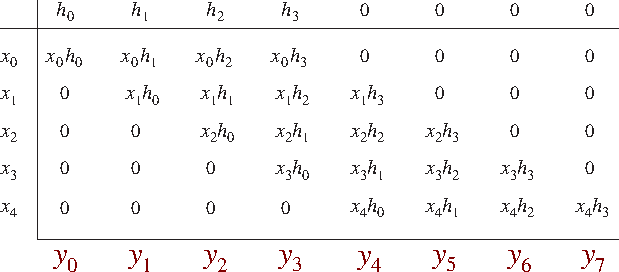
\includegraphics[width = 0.9\textwidth]{pic/LTITab.pdf}
		\end{minipage}
		\begin{minipage}{0.3\textwidth}
		 	\fcolorbox{CadetRed}{white}{$y(n) = \mysum{m}{}{x(m)\cdot h(n-m)}$}
		\end{minipage}
	\subsection{Matrix Form}
		Die Faltung zwischen Eingangsvektor $x(n)$ und Impulsantwort $h(n)$ kann auch als Matrixmultiplikation geschriben werden. Dabei gibt es zwei Formen:
		\begin{itemize}
		 \item Impulsantwortmatrix$\qquad\quad\;$\fcolorbox{CadetRed}{white}{$\vec y = H\cdot\vec x$}
		 \item Eingangssequenzmatirx $\qquad$\fcolorbox{CadetRed}{white}{$\vec y = X\cdot\vec h$}\\
		\end{itemize}
		
		\begin{minipage}{0.5\textwidth}
			\textbf{Impulsantwortmatrix \bm{$H\; ((L_x+M)\times L_x)$} }\\[0.2cm]
			$\begin{bmatrix} \;y_0\;\;\\y_1\\y_2\\y_3\\y_4\\y_5\\y_6\\y_7\end{bmatrix} = \underbrace{\begin{bmatrix} \;h_0\;\; & 0 & 0 & 0 & 0\\ h_1&\;h_0\;\;&0&0&0\\h_2&h_1&\;h_0\;\;&0&0\\h_3&h_2&h_1&\;h_0\;\;&0\\0&h_3&h_2&h_1&\;h_0\;\;\\0&0&h_3&h_2&h_1\\0&0&0&h_3&h_2\\0&0&0&0&h_3\end{bmatrix}}_{H}\cdot \begin{bmatrix} \;x_0\;\;\\x_1\\x_2\\x_3\\x_4\end{bmatrix}$
		\end{minipage}
		\begin{minipage}{0.5\textwidth}
			\textbf{Eingangssequenzmatirx \bm{$X\; ((L_x+M)\times (M+1))$} }\\[0.2cm]
			$\begin{bmatrix} \;y_0\;\;\\y_1\\y_2\\y_3\\y_4\\y_5\\y_6\\y_7\end{bmatrix} = \underbrace{\begin{bmatrix} \;x_0\;\; & 0 & 0 & 0\\ x_1&\;x_0\;\;&0&0\\x_2&x_1&\;x_0\;\;&0\\x_3&x_2&x_1&\;x_0\;\;\\x_4&x_3&x_2&x_1&\\0&x_4&x_3&x_2\\0&0&x_4&x_3&\\0&0&0&x_4&\end{bmatrix}}_{X}\cdot \begin{bmatrix} \;h_0\;\;\\h_1\\h_2\\h_3\end{bmatrix}$
		\end{minipage}
	
\newpage
	\subsection{Overlap-Add Blockfaltung}
		\vspace*{-0.2cm}\begin{minipage}{0.4\textwidth}
			Wenn die Eingangssequenz sehr lange wird muss diese in Blöcke der Länge $L_x$ aufgeteilt werden. Jeder dieser Blöcke wird einzeln verarbeitet. Da durch die Faltung aber Ausgangblöcke entstehen, die länger sind als die Eingangsblöcke, müssen diese auf die Länge der Eingangsblöcke $L_x$ zugeschnitten werden. der Rest des Ausgangsblockes $y_{temp}$ zum nächsten Blockes addiert.
		\end{minipage}
		\begin{minipage}{0.03\textwidth}$ $\end{minipage}
		\begin{minipage}{0.55\textwidth}
			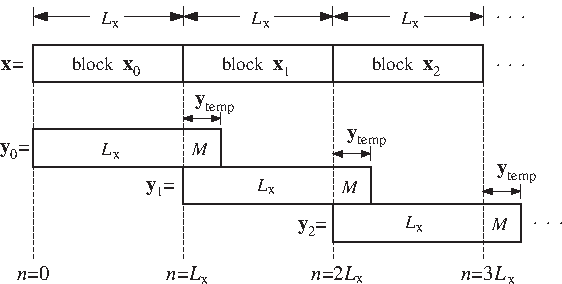
\includegraphics[width = 1\textwidth]{pic/overlapConv.pdf}
		\end{minipage}

	\subsection{Generelle Faltung}
		Für akausale Eingangssequenzen und akausale Impulsantworten gilt folgende allgemeine Faltungsformel:\\[0.2cm]
		\begin{minipage}{0.57\textwidth}
			Direct-Form:$\qquad$\fcolorbox{CadetRed}{white}{$y(n) = \mysum{m = max\{-M_1,n-L_2+1\}}{min\{n+L_1,M_2\}}{h(m)\cdot x(n-m)}$}\\[0.2cm]
		\end{minipage}
		\begin{minipage}{0.03\textwidth}$ $\end{minipage}
		\begin{minipage}{0.4\textwidth}
			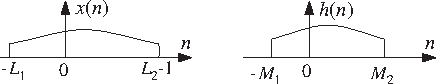
\includegraphics[width = 1\textwidth]{pic/genConv.pdf}
		\end{minipage}
		
	\subsection{DC-Gain}
		Der DC-Gain eines stabilen Filters ist der Wert, auf den der Ausgang konvergiert, wenn am Eingang der Einheitsschritt angelegt wird $x(n) = u(n)$\\[0.2cm]
		\textbf{DC-Gain}$\qquad$\fcolorbox{CadetRed}{white}{$y_{DC} = \mysum{m}{}{h(m)}$}\\[0.4cm]
		
\section{Sample für Sample Verarbeitung}
	\vspace*{-0.8cm}\begin{minipage}{0.65\textwidth}
		\begin{itemize}
		\item Die Sample für Sample Verarbeitung wird angewendet wenn zwischen Ein- und Ausgang nur eine kurze Verzögerungszeit liegen darf (Echtzeitsysteme).\\[-0.4cm]
		\item Diese Verarbeitung kann in Signalflussdiagrammen dargestellt werden. Dazu werden die drei Elemente Addierer, Verstärker und Verzögerer verwendet.
		\end{itemize}
	\end{minipage}
	\begin{minipage}{0.05\textwidth}$ $\end{minipage}
	\begin{minipage}{0.3\textwidth}
		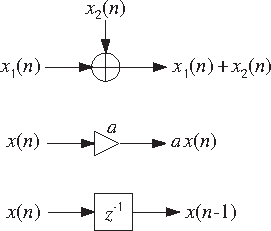
\includegraphics[width = 1\textwidth]{pic/sampleSample.pdf}
	\end{minipage}\\[-0.5cm]
		
	\subsection{Verzögerung (Pure Delays)}
		Um die verzögerte Werte speichern zu können werden \textbf{Zustände} definiert.\\ Ein Zustand $w(n)$ ist ein Register, welches den vorhergehenden Wert (Zustand) speichert. \\[0.2cm]
		\begin{danger}
		 Die Reihenfolge der Register-Updates ist sehr wichtig!
		\end{danger}\\[0.3cm]
		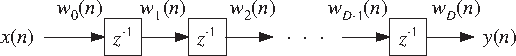
\includegraphics[width = 0.6\textwidth]{pic/delayD.pdf}\\[0.4cm]
		\begin{minipage}{0.3\textwidth}
			\textbf{I/O Gleichungen}\\[0.2cm]
			\begin{tabular}{|l|}
			\hline $ $\\[-0.3cm]
				$w_0(n) = x(n)$\\
				$y(n) = w_D(n)$\\[0.2cm]
				for $i = D,D-1,..,1$ do:\\
				$w_i(n+1) = w_{i-1}(n)$\\[0.2cm]
			\hline     
			\end{tabular}
		\end{minipage}
		\begin{minipage}{0.4\textwidth}
			\textbf{Algorithums}\\[0.2cm]
			\begin{tabular}{|l|}
			\hline $ $\\[-0.3cm]
				$w[0] = x;$\\
				$y = w[D]; $\\[0.2cm]
				for $i = D,D-1,..,1$ do:\\
				$w[i] = w[i-1];$\\[0.2cm]
			\hline     
			\end{tabular} 
		\end{minipage}

\newpage
	\subsection{FIR filtern mit Direktform}
		\begin{minipage}{0.5\textwidth}
			Die Direktform I/O Faltungsformel für ein FIR-Filter der Ordung $M$ lautet:\\[0.2cm]
			\fcolorbox{CadetRed}{white}{$\begin{array}{lcl}y(n)& =& h_0x(n) + h_1x(n-1) + ... + h_Mx(n-M)\\[0.2cm]& =& h_0w_0(n) + h_1w_1(n) + ... + h_Mw_M(n)\end{array}$}\\[0.4cm]
			Diese Form kann direkt in ein Signalflussdiagramm umgesetzt werden. Dabei gelten folgende Beziehungen:\\[0.2cm]
			\fcolorbox{CadetRed}{white}{$\begin{array}{l}w_0(n) = x(n)\\w_1(n) = x(n-1) = w_0(n-1)\\w_2(n) = x(n-2) = w_1(n-1)\\\vdots\\w_M(n) = x(n-M) = w_{M-1}(n-1)\end{array}$}
		\end{minipage}\begin{minipage}{0.03\textwidth}$ $\end{minipage}
		\begin{minipage}{0.4\textwidth}
			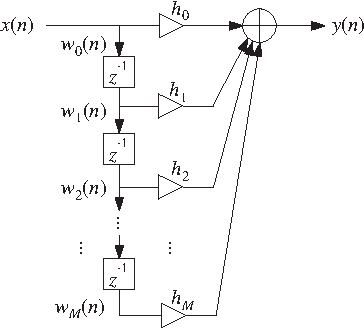
\includegraphics[width = \textwidth]{pic/firFlussdiagramm.pdf}
		\end{minipage}\\[0.2cm]

		\begin{itemize}
		 \item Durch die Verwendung von internen Zuständen kann der Ausgang aus dem aktuellen Eingangswert und den Zuständen berechnet werden.
		 \item Die input-on und input-off Transienten können anhand des Signalflussdiagrammes leicht erklärt werden. Sie entsprechen jeweils der Zeit (Anzahl Samples), bis die Verzögerungslinie (Zustände) gefüllt bzw. geleert sind.\\[-0.2cm]
		\end{itemize}
		\begin{minipage}{0.5\textwidth}
			\textbf{I/O Gleichungen}\\[0.2cm]
			\begin{tabular}{|l|}
			\hline $ $\\[-0.3cm]
				$w_0(n) = x(n)$\\
				$y(n) = h_0w_0(n) + h_1w_1(n) + ... + h_Mw_M(n)$\\[0.2cm]
				for $i = M,M-1,..,1$ do:\\
				$w_i(n+1) = w_{i-1}(n)$\\[0.2cm]
			\hline     
			\end{tabular}
		\end{minipage}
		\begin{minipage}{0.4\textwidth}
			\textbf{Algorithums}\\[0.2cm]
			\begin{tabular}{|l|}
			\hline $ $\\[-0.3cm]
				$w[0] = x;$\\
				$y = h[0]\,w[0] + h[1]\,w[1] + ... + h[M]\,w[M]; $\\[0.2cm]
				for $i = M,M-1,..,1$ do:\\
				$w[i] = w[i-1];$\\[0.2cm]
			\hline     
			\end{tabular} 
		\end{minipage}

\chapter{z-Transformation  \textcolor{black}{\small S.183}}
% 
% (c) Copyright 2016 Tabea Mendez
% 
% This source is free: you can redistribute it and/or modify
% it under the terms of the GNU General Public License as published by
% the Free Software Foundation, either version 3 of the License, or
% (at your option) any later version.
% 
% This source is distributed in the hope that it will be useful,
% but WITHOUT ANY WARRANTY; without even the implied warranty of
% MERCHANTABILITY or FITNESS FOR A PARTICULAR PURPOSE.  See the
% GNU General Public License for more details.
% 
% You should have received a copy of the GNU General Public License
% along with this source.  If not, see <http://www.gnu.org/licenses/>.
%
%%%%%%%%%%%%%%%%%%%%%%%%%%%%%%%%%%%%%%%%%%%%%%%%%%%%%%%%%%%%%%%%%%%%%%%%%%%%%%

\begin{description}
 \item [Definition:]$ $\\[0.2cm]
	\fcolorbox{CadetRed}{white}{$X(z) = \mysum{n=-\infty}{\infty}{x(n)\cdot z^{-n}}$}
 \item [Linearität:] Die z-Transformation ist linear.\\[0.2cm]
	\fcolorbox{CadetRed}{white}{$a_1\,x_1(n) + a_2\,x_2(n)\qquad\xrightarrow {\;\;\;Z\;\;\;}\qquad a_1\,X_1(z) + a_2\,X_2(z)$}
 \item [Verzögerung:] Verzögerung in der Zeit entsprich einer Multipikation mit $z^{-D}$ in der z-Transformation.\\[0.2cm]
	\fcolorbox{CadetRed}{white}{$x(n)\quad\xrightarrow {\;\;Z\;\;}\quad X(z)\qquad\Rightarrow \qquad x(n-D)\quad\xrightarrow {\;\;Z\;\;}\quad X(z)\cdot z^{-D}$}
 \item [Faltung:] Die Faltung in der Zeit entsprich der Multipikation in der z-Transformation\\[0.2cm]
	\fcolorbox{CadetRed}{white}{$y(n)=h(n)\ast x(n)\qquad\xrightarrow {\;\;\;Z\;\;\;}\qquad Y(z)=H(z)\cdot X(z)$}
\end{description}

\section{Konvergenzbereich (ROC)}
	Zum Konvergenzbereich (Region of Convergence) gehören alle komplexen z-Werte bei denen die z-Transformation einen endlichen Wert hat.\\[0cm]
	\textbf{Region of Convergence:}$\qquad$\fcolorbox{CadetRed}{white}{ROC $= \left\{z\in\mathbb{C}\;\left|\;X(z) = \mysum{n=-\infty}{\infty}{x(n)\cdot z^{-n}}\neq\pm \infty\right.\right\}$}\\[0.4cm]
	Zu einer z-Transformation muss \textbf{immer die ROC angegeben} werden. Ist keine ROC angegeben wird angenommen, dass das Zeitsignal kausal war. Hat eine z-Transformation keine ROC, so existiert diese nicht!\\[0.2cm]
	\fcolorbox{CadetRed}{white}{$\begin{array}{rcl}a^n\,u(n) \quad\xrightarrow{\;\; Z \;\;}\quad\dfrac{1}{1-a\,z^{-1}} && \text{ROC} = \left\{z\in\mathbb{C}\;\left|\;|z|>|a|\right.\right\}\\[0.5cm]-a^n\,u(-n-1) \quad\xrightarrow{\;\; Z \;\;}\quad\dfrac{1}{1-a\,z^{-1}} &\qquad\qquad& \text{ROC} = \left\{z\in\mathbb{C}\;\left|\;|z|<|a|\right.\right\}\end{array}$}$\quad$\fcolorbox{white}{white}{$\begin{array}{l}\rightarrow\quad\text{kausales Signal}\\[0.7cm]\rightarrow\quad\text{antikausales Signal}\end{array}$}\\[0.2cm]
	
	\begin{tikzpicture}[>=latex', scale=1.4]
		\def\s{3};
		\def\f{1.2};
		\def\r{0.8};

		\coordinate (c1) at (0,0);
		\draw[line width=0.75,fill=CadetRed, opacity=0.5](c1)++(-\s/2,-\s/2)--++(\s,0)--++(0,\s)--++(-\s,0)--cycle ;
		\draw[line width=0.75](c1)++(-\s/2,-\s/2)node[above right]{kausal}--++(\s,0)--++(0,\s)node[below left]{$z$-Plane}--++(-\s,0)--cycle node[below right, CadetRed]{\textbf{ROC}};

		\draw[line width=0.75,fill=white](c1)--++(-\f,0)--++(2*\f,0)--++(-\f,0)--++(0,-\f)--++(0,2*\f)--++(0,-\f)circle(\r);

		\draw[line width=0.75,fill](c1)++(-\f,0.7)circle(\r/30)node[above]{$z$};
		\draw[line width=0.75,->](c1)--node[rotate=-30, above right]{\footnotesize$|z|$}++(-\f,0.7);

		\draw[line width=0.75,fill](c1)++({\r*cos(30)},{\r*sin(30)})circle(\r/20)node[above right=-1pt,black]{$a$};%node[rotate=30,CadetRed]{\bm{$\times$}};
		\draw[line width=0.75,->](c1)--node[rotate=30, above ]{\footnotesize$|a|$}++({\r*cos(30)},{\r*sin(30)});


	\end{tikzpicture} $\qquad$
	\begin{tikzpicture}[>=latex', scale=1.4]
		\def\s{3};
		\def\f{1.2};
		\def\r{0.8};

		\coordinate (c1) at (0,0);
		\draw[line width=0.75,fill=white, opacity=0.5](c1)++(-\s/2,-\s/2)--++(\s,0)--++(0,\s)--++(-\s,0)--cycle ;
		\draw[line width=0.75](c1)++(-\s/2,-\s/2)node[above right]{antikausal}--++(\s,0)--++(0,\s)node[below left]{$z$-Plane}--++(-\s,0)--cycle node[below right, CadetRed]{\textbf{ROC}};

		\draw[line width=0.75,fill=CadetRed, opacity=0.5](c1)--++(-\f,0)--++(2*\f,0)--++(-\f,0)--++(0,-\f)--++(0,2*\f)--++(0,-\f)circle(\r);
		\draw[line width=0.75](c1)--++(-\f,0)--++(2*\f,0)--++(-\f,0)--++(0,-\f)--++(0,2*\f)--++(0,-\f)circle(\r);


		\draw[line width=0.75,fill](c1)++(-\f/2,0.2)circle(\r/30)node[above]{$z$};
		\draw[line width=0.75,->](c1)--node[rotate=-20, above]{\footnotesize$|z|$}++(-\f/2,0.2);

		\draw[line width=0.75,fill,black](c1)++({\r*cos(30)},{\r*sin(30)})circle(\r/20)node[above right=-1pt,black]{$a$};%node[rotate=30,CadetRed]{\bm{$\times$}};
		\draw[line width=0.75,->](c1)--node[rotate=30, above ]{\footnotesize$|a|$}++({\r*cos(30)},{\r*sin(30)});


	\end{tikzpicture}\\[0.cm]
	

\section{Kausalität und Stabilität}
	\begin{minipage}{0.5\textwidth}
		\textbf{Stabilitätsbedinung}\\[0.2cm]
		\fcolorbox{CadetRed}{white}{\parbox{6.5cm}{Der \textbf{Einheitskreis} der z-Ebene muss\\ \textbf{innerhalb} der ROC liegen!}}\\[0.3cm]
		\begin{tikzpicture}[>=latex', scale=1.1]
			\def\s{3};
			\def\f{1.3};
			\def\r{0.7};

			\coordinate (c1) at (0,0);
			\draw[line width=0.75](c1)++(-\s/2,-\s/2)node[above right]{ }--++(\s,0)--++(0,\s)node[below left]{$z$-Plane}--++(-\s,0)--cycle node[below right, CadetRed]{\textbf{ROC}};

			\draw[line width=0.75,fill=white](c1)--++(-\f,0)--++(2*\f,0)--++(-\f,0)--++(0,-\f)--++(0,2*\f);

			\draw[line width=1.5,dashed,CadetRed](c1)circle(0.9);
			\draw[line width=1.5,CadetRed](c1)++(0.9,0.1)--++(0,-0.2)node[below right=-1pt]{1};
		\end{tikzpicture}
	\end{minipage}
	\begin{minipage}{0.5\textwidth}
		\textbf{Grenzstabil}\\[0.2cm]
		\fcolorbox{CadetRed}{white}{\parbox{8.5cm}{Der Einheitskreis bildet die Grenze der der ROC$\quad\rightarrow\quad$ Pol liegt genau auf dem Einheitskreis!}}\\[0.3cm]
		\begin{tikzpicture}[>=latex', scale=1.1]
			\def\s{3};
			\def\f{1.3};
			\def\r{0.7};

			\coordinate (c1) at (0,0);
			\draw[line width=0.75](c1)++(-\s/2,-\s/2)node[above right]{ }--++(\s,0)--++(0,\s)node[below left]{$z$-Plane}--++(-\s,0)--cycle node[below right, CadetRed]{\textbf{ }};

			\draw[line width=0.75,fill=white](c1)--++(-\f,0)--++(2*\f,0)--++(-\f,0)--++(0,-\f)--++(0,2*\f);

			\draw[line width=1.5,dashed,CadetRed](c1)circle(0.9);
			\draw[line width=1.5,CadetRed](c1)++(0.9,0.1)--++(0,-0.2)node[below right=-1pt]{1};

			\draw[line width=0.75,fill,](c1)++(0.67,0.6)circle(\r/10)node[below left=0pt,black]{$p$};

		\end{tikzpicture}
	\end{minipage}
\newpage
	\subsection{Kausale Signale}
	\vspace*{-0.3cm}\begin{minipage}{0.43\textwidth}
		\textbf{Generelles kausales Signal: }\\[0.2cm]
		\fcolorbox{CadetRed}{white}{$\begin{array}{c}x(n) = A_1\,p_1^n\,u(n) + A_2\,p_2^n\,u(n) + ...\\[0.2cm]\text{\huge$\downarrow$}\;Z\\[0.1cm] X(z) = \dfrac{A_1}{1-p_1\,z^{-1}} + \dfrac{A_2}{1-p_2\,z^{-1}} + ...\end{array}$}\\[0.3cm]
	\end{minipage}
	\begin{minipage}{0.33\textwidth}
		\textbf{ROC: }$\,\,\;\;\;\quad$\\[0.2cm]\fcolorbox{CadetRed}{white}{ROC $= \left\{z\in\mathbb{C}\;\left|\;|z|>\max\limits_{i}^{}{|p_i|}\right.\right\}$}\\[0.2cm]
		\textbf{Stabilitätsbedinung:}$\qquad$\\[0.2cm]\fcolorbox{CadetRed}{white}{$\max\limits_{i}^{}{|p_i|}<1$}\\[-0.07cm]
	\end{minipage}
	\begin{minipage}{0.4\textwidth}
		\begin{tikzpicture}[>=latex', scale=1.4]
			\def\s{3};
			\def\f{1.3};
			\def\r{0.7};

			\coordinate (c1) at (0,0);
			\draw[line width=0.75,fill=CadetRed, opacity=0.5](c1)++(-\s/2,-\s/2)--++(\s,0)--++(0,\s)--++(-\s,0)--cycle ;
			\draw[line width=0.75](c1)++(-\s/2,-\s/2)node[above right]{kausal}--++(\s,0)--++(0,\s)node[below left]{$z$-Plane}--++(-\s,0)--cycle node[below right, CadetRed]{\textbf{ROC}};

			\draw[line width=0.75,fill=white](c1)--++(-\f,0)--++(2*\f,0)--++(-\f,0)--++(0,-\f)--++(0,2*\f)--++(0,-\f)circle(\r);

			\draw[line width=0.75,dashed](c1)--++(-\f,0)--++(2*\f,0)--++(-\f,0)--++(0,-\f)--++(0,2*\f)--++(0,-\f)circle(0.9);
			\draw[line width=0.75](c1)++(0.9,0.1)--++(0,-0.2)node[below right=-1pt]{1};

			\draw[line width=0.75,fill,](c1)++(0.35,0.6)circle(\r/15)node[below left=-2pt,black]{$p_4$};
			\draw[line width=0.75,fill,](c1)++(0.2,0)circle(\r/15)node[above right=-1pt,black]{$p_2$};
			\draw[line width=0.75,fill,](c1)++(0.35,-0.5)circle(\r/15)node[above left=-2pt,black]{$p_1$};
			\draw[line width=0.75,fill,](c1)++(-0.3,0.2)circle(\r/15)node[above=-1pt,black]{$p_3$};
		\end{tikzpicture}
	\end{minipage}\\[-0.3cm]

	\subsection{Antikausale Signale}
	\vspace*{-0.3cm}\begin{minipage}{0.43\textwidth}
		\textbf{Generelles antikausales Signal: }\\[0.2cm]
		\fcolorbox{CadetRed}{white}{$\begin{array}{c}x(n) = \text{-}B_1\,q_1^n\,u(\text{-}n\text{-}1) - B_2\,q_2^n\,u(\text{-}n\text{-}1) - ...\\[0.2cm]\text{\huge$\downarrow$}\;Z\\[0.1cm] X(z) = \dfrac{B_1}{1-q_1\,z^{-1}} + \dfrac{B_2}{1-q_2\,z^{-1}} + ...\end{array}$}\\[0.3cm]
	\end{minipage}
	\begin{minipage}{0.33\textwidth}
		\textbf{ROC: }$\,\,\;\;\;\quad$\\[0.2cm]\fcolorbox{CadetRed}{white}{ROC $= \left\{z\in\mathbb{C}\;\left|\;|z|<\min\limits_{i}^{}{|q_i|}\right.\right\}$}\\[0.2cm]
		\textbf{Stabilitätsbedinung:}$\qquad$\\[0.2cm]\fcolorbox{CadetRed}{white}{$\min\limits_{i}^{}{|q_i|}>1$}\\[-0.15cm]
	\end{minipage}
	\begin{minipage}{0.4\textwidth}
		\begin{tikzpicture}[>=latex', scale=1.4]
			\def\s{3};
			\def\f{1.3};
			\def\r{1.1};

			\coordinate (c1) at (0,0);
			\draw[line width=0.75,fill=white, opacity=0.5](c1)++(-\s/2,-\s/2)--++(\s,0)--++(0,\s)--++(-\s,0)--cycle ;
			\draw[line width=0.75](c1)++(-\s/2,-\s/2)node[above right]{kausal}--++(\s,0)--++(0,\s)node[below left]{$z$-Plane}--++(-\s,0)--cycle node[below right, CadetRed]{\textbf{ROC}};

			\draw[line width=0.75,fill=CadetRed, opacity=0.5](c1)--++(-\f,0)--++(2*\f,0)--++(-\f,0)--++(0,-\f)--++(0,2*\f)--++(0,-\f)circle(\r);
			\draw[line width=0.75](c1)--++(-\f,0)--++(2*\f,0)--++(-\f,0)--++(0,-\f)--++(0,2*\f)--++(0,-\f)circle(\r);


			\draw[line width=0.75,dashed](c1)--++(-\f,0)--++(2*\f,0)--++(-\f,0)--++(0,-\f)--++(0,2*\f)--++(0,-\f)circle(0.9);
			\draw[line width=0.75](c1)++(0.9,0.1)--++(0,-0.2)node[below left=-1pt,yshift=4pt]{1};
			\def\r{0.7};

			\draw[line width=0.75,fill,](c1)++(0.85,0.7)circle(\r/15)node[above right=-1pt,black]{$q_4$};
			\draw[line width=0.75,fill,](c1)++(1.3,0)circle(\r/15)node[above=-0pt,black]{$q_2$};
			\draw[line width=0.75,fill,](c1)++(0.8,-1.2)circle(\r/15)node[right=-0pt,black]{$q_1$};
			\draw[line width=0.75,fill,](c1)++(-1.3,0.4)circle(\r/15)node[above=-1pt,black]{$q_3$};
		\end{tikzpicture}
	\end{minipage}\\[-0.3cm]
	
	\subsection{Gemischte Signale}
	\begin{minipage}[t]{0.43\textwidth}
		\textbf{Generelles gemischtes Signal: }\\[0.2cm]
		\fcolorbox{CadetRed}{white}{$\begin{array}{c}x(n) = A_1\,p_1^n\,u(n) + A_2\,p_2^n\,u(n) + ...\text{\textcolor{white}{$xn\;\;\;\;$}}\\[0.2cm]\text{\textcolor{white}{$x(n)\;\,\;\;$}} \text{-}B_1\,q_1^n\,u(\text{-}n\text{-}1) - B_2\,q_2^n\,u(\text{-}n\text{-}1) - ...\\[0.2cm]\text{\huge$\downarrow$}\;Z\\[0.1cm] X(z) = \dfrac{A_1}{1-p_1\,z^{-1}} + \dfrac{A_2}{1-p_2\,z^{-1}} + ...\\[0.5cm] \text{\textcolor{white}{$X(z)$}} + \dfrac{B_1}{1-q_1\,z^{-1}} + \dfrac{B_2}{1-q_2\,z^{-1}} + ...\end{array}$}\\[0.3cm]
	\end{minipage}
	\begin{minipage}[t]{0.6\textwidth}
		\textbf{ROC: }$\,\,\;\;\;\quad$\\[0.275cm]\fcolorbox{CadetRed}{white}{ROC $= \left\{z\in\mathbb{C}\;\left|\;|z|>\max\limits_{i}^{}{|p_i|\quad\cap\quad|z|<\min\limits_{i}^{}{|q_i|}}\right.\right\}$}\\[0.2cm]
		\textbf{Stabilitätsbedinung:}$\qquad$\\[0.2cm]\fcolorbox{CadetRed}{white}{$\max\limits_{i}^{}{|p_i|}<1\quad\cap\quad\min\limits_{i}^{}{|q_i|}>1$}\\[-0.025cm]
	\end{minipage}\\[-3.2cm]
	\hspace*{14.05cm}\begin{minipage}{0.4\textwidth}
		\begin{tikzpicture}[>=latex', scale=1.4]
			\def\s{3};
			\def\f{1.3};
			\def\r{1.1};

			\coordinate (c1) at (0,0);
			\draw[line width=0.75,fill=white, opacity=0.5](c1)++(-\s/2,-\s/2)--++(\s,0)--++(0,\s)--++(-\s,0)--cycle ;
			\draw[line width=0.75](c1)++(-\s/2,-\s/2)node[above right]{kausal}--++(\s,0)--++(0,\s)node[below left]{$z$-Plane}--++(-\s,0)--cycle node[below right, CadetRed]{\textbf{ROC}};

			\draw[line width=0.75,fill=CadetRed, opacity=0.5](c1)--++(-\f,0)--++(2*\f,0)--++(-\f,0)--++(0,-\f)--++(0,2*\f)--++(0,-\f)circle(\r);
			\draw[line width=0.75](c1)--++(-\f,0)--++(2*\f,0)--++(-\f,0)--++(0,-\f)--++(0,2*\f)--++(0,-\f)circle(\r);

			\def\r{0.7};
			\draw[line width=0.75,fill=white](c1)--++(-\f,0)--++(2*\f,0)--++(-\f,0)--++(0,-\f)--++(0,2*\f)--++(0,-\f)circle(\r);

			\draw[line width=0.75,dashed](c1)--++(-\f,0)--++(2*\f,0)--++(-\f,0)--++(0,-\f)--++(0,2*\f)--++(0,-\f)circle(0.9);
			\draw[line width=0.75](c1)++(0.9,0.1)--++(0,-0.2)node[below right=-3pt,yshift=2pt]{1};

			\draw[line width=0.75,fill,](c1)++(0.85,0.7)circle(\r/15)node[above right=-1pt,black]{$q_2$};
			\draw[line width=0.75,fill,](c1)++(-1.3,0.4)circle(\r/15)node[above=-1pt,black]{$q_1$};

			\draw[line width=0.75,fill,](c1)++(0.2,0)circle(\r/15)node[above right=-1pt,black]{$p_2$};
			\draw[line width=0.75,fill,](c1)++(0.41,-0.56)circle(\r/15)node[above left=-2pt,black]{$p_1$};
		\end{tikzpicture}
	\end{minipage}\\[-0.8cm]

	
\section{Inverse z-Transformation}
	Um eine z-Transformation, die als \textbf{gebrochen rationale Funktion} dargestellt werden kann, in die Zeit zurückzutransformieren sind folgende Schritte notwendig:
	\begin{itemize}
	 \item Die z-Transformation in Partialbrüche der Form $\dfrac{1}{1-a\,z^{-1}}$ zerlegen
	 \item Jeden Partialbruch mit Hilfe folgender Beziehung und dem Wissen, ob der Pol kausal oder anitkausal ist, zurückzutransformieren.\\[0.2cm]
	\fcolorbox{white}{white}{$\begin{array}{lr}\text{kausales Signal}&\quad\rightarrow\\[0.7cm]\text{antikausales Signal}&\quad\rightarrow\end{array}$}$\quad$\fcolorbox{CadetRed}{white}{$\begin{array}{rcl}a^n\,u(n) \quad\xrightarrow{\;\; Z \;\;}\quad\dfrac{1}{1-a\,z^{-1}} && \text{ROC} = \left\{z\in\mathbb{C}\;\left|\;|z|>|a|\right.\right\}\\[0.5cm]-a^n\,u(-n-1) \quad\xrightarrow{\;\; Z \;\;}\quad\dfrac{1}{1-a\,z^{-1}} &\qquad\qquad& \text{ROC} = \left\{z\in\mathbb{C}\;\left|\;|z|<|a|\right.\right\}\end{array}$}
	\item Bei Doppelpolen folgende Rücktransformationen verwenden.\\[0.2cm]
	\fcolorbox{white}{white}{$\begin{array}{lr}\text{kausales Signal}&\rightarrow\\[0.7cm]\text{antikausales Signal}&\rightarrow\end{array}$}\fcolorbox{CadetRed}{white}{$\begin{array}{rcl}(n+1)\,a^n\,u(n) \quad\xrightarrow{\;\; Z \;\;}\quad\dfrac{1}{(1-a\,z^{-1})^2} && \text{ROC} = \left\{z\in\mathbb{C}\;\left|\;|z|>|a|\right.\right\}\\[0.5cm]-(n+1)\,a^n\,u(-n-1) \quad\xrightarrow{\;\; Z \;\;}\quad\dfrac{1}{(1-a\,z^{-1})^2} &\qquad& \text{ROC} = \left\{z\in\mathbb{C}\;\left|\;|z|<|a|\right.\right\}\end{array}$}
	 \item Konstanten werden zu gewichteten Diracs zurücktransformiert.$\qquad$ \fcolorbox{CadetRed}{white}{$ A_0 \delta(n) \xrightarrow{\;\;Z\;\;} A_0$}
	\end{itemize}
	
	\subsection{Partialbruchzerlegung bei einfachen Polen}
		Bei der Partialbruchzerlegung einer gebrochen rationalen Funktion werden drei Fälle unterschieden:\\[0.3cm]
		\begin{minipage}{0.4\textwidth}
			\begin{itemize}
			\item $M > N\quad$ echt gebrochen\\[-0.35cm]
			\item $M = N\quad$ unecht gebrochen\\[-0.35cm]
			\item $M < N\quad$ unecht gebrochen\\[-0.35cm]
			\end{itemize}
		\end{minipage}
		\begin{minipage}{0.3\textwidth}
			\fcolorbox{CadetRed}{white}{$X(z) = \dfrac{N(z)}{D(z)} = \dfrac{b_0 + b_1\,z^{-1} + b_2\,z^{-2} + \dots + b_N\,z^{-N} }{1 + a_1\,z^{-1} + a_2\,z^{-2} + \dots + a_M\,z^{-M} }$}
		\end{minipage}

		\begin{tabularx}{\textwidth}{|p{1.6cm}|X|}
		 \hline&\\[-0.3cm]
			\bm{$M > N$}
			& $X(z) = \dfrac{N(z)}{D(z)} = \dfrac{N(z)}{(1 - p_1\,z^{-1})\,\dots\,(1 - p_M\,z^{-1}) } = \dfrac{A_1}{(1 - p_1\,z^{-1})} + \dots + \dfrac{A_M}{(1 - p_M\,z^{-1})}$\\[0.6cm]
			&\fcolorbox{CadetRed}{white}{$A_i = \left[(1 - p_i\,z^{-1})\cdot X(z)\right]_{z=p_i} = \left[\dfrac{N(z)}{\myprod{j\neq i}{}{(1 - p_j\,z^{-1})}}\right]_{z=p_i}$}\\[1cm]
		 \hline&\\[-0.3cm]
			\bm{$M = N$} & $X(z) = \dfrac{N(z)}{D(z)} = \dfrac{N(z)}{(1 - p_1\,z^{-1})\,\dots\,(1 - p_M\,z^{-1}) } = A_0 + \dfrac{A_1}{(1 - p_1\,z^{-1})} + \dots + \dfrac{A_M}{(1 - p_M\,z^{-1})}$\\[0.6cm]
			&\fcolorbox{CadetRed}{white}{$A_0 = X(z)|_{z=0} $}$\quad\qquad$\fcolorbox{CadetRed}{white}{$A_i$ siehe Fall $M>N$}\\[0.3cm]
		 \hline&\\[-0.3cm]
			\bm{$M < N$} & $X(z) = \dfrac{N(z)}{D(z)}\;\overset{\text{Polynom-}}{\underset{\text{division}}{=}} \; Q(z) + \dfrac{R(z)}{D(z)}$\\[0.6cm]
			& $Q(z) = B_0 + B_1\,z^{-1} + ... + B_{N-M}\,z^{-(N-M)}\quad\xrightarrow{\;\; Z^{-1}\;\;}\quad B_0\,\delta(n) + \,\delta(n\text{-}1) + ... + B_{N-M}\,\delta(n\text{-}(N\text{-}M))$\\[0.4cm]
			& $\dfrac{R(z)}{D(z)} = \dfrac{R(z)}{(1 - p_1\,z^{-1})\,\dots\,(1 - p_M\,z^{-1}) } = \dfrac{A_1}{(1 - p_1\,z^{-1})} + \dots + \dfrac{A_M}{(1 - p_M\,z^{-1})}$\\[0.6cm]
			&\fcolorbox{CadetRed}{white}{$A_i$ siehe Fall $M>N$}\\[0.3cm]
		 \cline{2-2}&\\[-0.3cm]
			& $X(z) = \dfrac{N(z)}{D(z)} = N(z)\cdot W(z) $\\[0.4cm]
			& \fcolorbox{CadetRed}{white}{Nur $W(z)$ wie im Fall $M>N$ zurücktransformierten$\quad\Rightarrow\quad w(n)$}\\[0.4cm]
			& $W(z) = \dfrac{1}{D(z)} = \dfrac{1}{(1 - p_1\,z^{-1})\,\dots\,(1 - p_M\,z^{-1}) } = \dfrac{A_1}{(1 - p_1\,z^{-1})} + \dots + \dfrac{A_M}{(1 - p_M\,z^{-1})}$\\[0.5cm]
			&\fcolorbox{CadetRed}{white}{$A_i$ siehe Fall $M>N$}\\[0.4cm]
			& $X(z) = N(z)\cdot W(z) = b_0\cdot W(z) + b_1\,z^{-1}\cdot W(z) + b_2\,z^{-2}\cdot W(z) + \dots + b_N\,z^{-N}\cdot W(z)$\\[0.4cm]
			& \fcolorbox{CadetRed}{white}{$x(n)$ ist die Summe der mit $b_i$ gewichteten und um $i$ verzögerten $w(n)$}\\[0.3cm]
		 \hline
		\end{tabularx}

\newpage
\section{Frequenzspektrum}
	Das Frequenzspektrum (DTFT) eines diskreten Signals $x(n)$ und ist definiert als:\\[0.2cm]
	\fcolorbox{CadetRed}{white}{$X(\omega) = \mysum{n=-\infty}{\infty}{x(n)\,\e^{-j\omega n}}$}$\qquad$ und die inverse DTFT als:$\qquad$\fcolorbox{CadetRed}{white}{$x(n) = \dfrac{1}{2\pi}\,\myint{-\pi}{\pi}{X(\omega)\,\e^{j\omega n}}{\omega}$}\\[0.2cm]

	\subsection{Vergleich zwischen analogem Signal \bm{$x(nT)$} und digitalen Signal \bm{$x(n)$}}
		\begin{tabularx}{\textwidth}{|p{3cm}|X|X|}
		\hline&&\\[-0.35cm]
			&\textbf{Analoges Signal \bm{$x(nT)$}} & \textbf{Diskretes Signal \bm{$x(n)$}}\\[0.05cm]
		\hline&&\\[-0.35cm]
			\textbf{DTFT}& $\hat X(f)=\mysum{n=-\infty}{\infty}{x(nT)\cdot \e^{-j2\pi fTn}}$ &$X(\omega) = \mysum{n=-\infty}{\infty}{x(n)\,\e^{-j\omega n}}$\\[0.35cm]
		\hline&&\\[-0.35cm]
			\textbf{Periode}& $f_s$  & $2\,\pi$ \\[0.05cm]
		\hline&&\\[-0.35cm]
			\textbf{inverse DTFT}&$x(nT)=\dfrac{1}{f_s}\,\myint{-f_s/2}{f_2/2}{\hat X(f)\cdot \e^{j2\pi fTn}}{f}$ &$x(n) = \dfrac{1}{2\pi}\,\myint{-\pi}{\pi}{X(\omega)\,\e^{j\omega n}}{\omega}$\\[0.45cm]
		\hline
		\end{tabularx}\\
	
	\subsection{Geometrische Interpretation des Frequenzganges}
		\begin{minipage}{0.44\textwidth}
			Der Frequenzgang $X(\omega)$ entspricht der Übertragungsfunktion $X(z)$ auf dem Einheitskreis:\\[0.3cm]
			\fcolorbox{CadetRed}{white}{$z=\e^{j\omega}$}$\qquad\Rightarrow\qquad$\fcolorbox{CadetRed}{white}{$X(\omega) = X(z)|_{z=\e^{j\omega}}$}\\[0.3cm]
			Damit der Frequenzgang existiert, muss der Einheitskreis \textbf{innerhalb der Region of Convergence (ROC)} liegen.
		\end{minipage}\begin{minipage}{0.03\textwidth}$ $\end{minipage}
		\begin{minipage}{0.27\textwidth}
			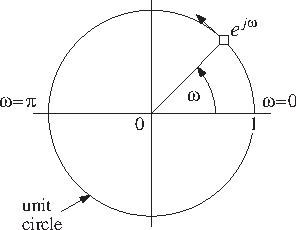
\includegraphics[width = 1\textwidth]{pic/geoFrequenzgang.pdf}\\
		\end{minipage}
		\begin{minipage}{0.26\textwidth}
			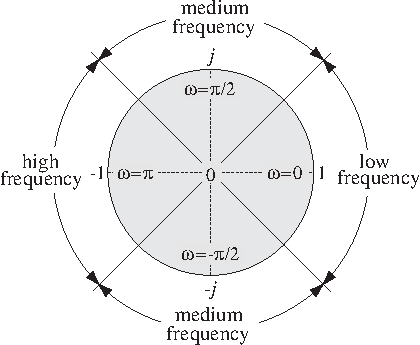
\includegraphics[width = 1\textwidth]{pic/frequency.pdf}
		\end{minipage}
		\begin{itemize}
			 \item Wenn $\omega$ von $-\pi$ bis $\pi$ variert, wendert $z$ auf dem Einheitskreis von $-1$ über $0$ nach $-1$.
			 \item Die tiefen Frequenzen sind bei $z \approx 1 $ und die hohen bei $z \approx -1 $. Bei $z \approx \pm j$ sind die mittleren Frequenzen.
		\end{itemize}$ $\\[-0.1cm]
		\begin{minipage}{0.7\textwidth}
			Anhand der Pol- und Nullstellen in der z-Ebene,\\ kann der Frequenzgang $|X(\omega)|$ skizziert werden.\\[0.3cm]
			\fcolorbox{CadetRed}{white}{$|X(\omega_0)| = \dfrac{\myprod{i}{\text{\textcolor{white}{a}}}{\text{Abstand von }\e^{j\omega_0}\text{ zur Nullstelle }z_i}}{\myprod{j}{\text{\textcolor{white}{a}}}{\text{Abstand von }\e^{j\omega_0}\text{ zum Pol }p_j}}$}\\[0.3cm]
			Daraus lassen sich folgende Grundsätze ableiten\\[-0.3cm]
			\begin{itemize}
				\item Je näher der Punkt auf dem Einheitskreis einer Nullstelle kommt,\\ desto kleiner wird der Frequenzgang.\\[-0.25cm]
				\item Je näher der Punkt auf dem Einheitskreis einem Pol kommt, desto\\ grösser wird der Frequenzgang.\\[-0.25cm]
				\item Sitzt der Pol genau auf dem Einheitskreis, so wird der Frequenzgang\\ an dieser stelle unendlich gross.
			\end{itemize}
		\end{minipage}
		\hspace*{-4cm}\begin{minipage}{0.5\textwidth}
			\vspace*{-0.5cm}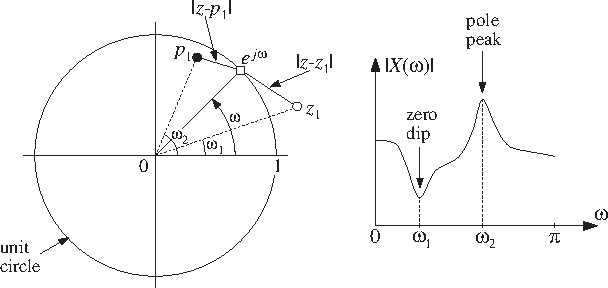
\includegraphics[width = 1\textwidth]{pic/geoFrequenzgangPN.pdf}\\
			\hspace*{3.5cm}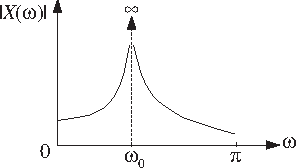
\includegraphics[width = 0.6\textwidth]{pic/polAufEinheitskreis.pdf}
		\end{minipage}$ $\\

	\subsection{Fourierpärchen}
		\vspace*{-0.2cm}\begin{minipage}{0.68\textwidth}
			\begin{tabular}{l|c|c}
				& $x(n)$ & $X(\omega)$ (Nyquistintervall)\\[0.1cm]
			\hline&&\\[-0.3cm]
				\text{Komplexe Schwingung} $\quad$& $\e^{j\omega_0 n}$ & $2\pi\,\delta(\omega-\omega_0)$\\[0.2cm]
				\text{Cosinusschwingung} & $\cos(\omega_0 n)$ & $\pi\,\delta(\omega-\omega_0) + \pi\,\delta(\omega+\omega_0)$\\[0.2cm]
				\text{Sinusschwingung} & $\sin(\omega_0 n)$ & $-j\pi\,\delta(\omega-\omega_0) + j\pi\,\delta(\omega+\omega_0)$\\[0.1cm]
			\hline
			\end{tabular}
		\end{minipage}
		\begin{minipage}{0.3\textwidth}
			\textbf{Satz des Parseval:}\\[0.2cm]\fcolorbox{CadetRed}{white}{$E = \mysum{n=-\infty}{\infty}{|x(n)|^2} = \dfrac{1}{2\pi}\,\myint{-\pi}{\pi}{|H(\omega)|^2}{\omega}$}\\
		\end{minipage}
	
	




\chapter{Übertragungsfunktionen \textcolor{black}{\small S.214}}
% 
% (c) Copyright 2016 Tabea Mendez
% 
% This source is free: you can redistribute it and/or modify
% it under the terms of the GNU General Public License as published by
% the Free Software Foundation, either version 3 of the License, or
% (at your option) any later version.
% 
% This source is distributed in the hope that it will be useful,
% but WITHOUT ANY WARRANTY; without even the implied warranty of
% MERCHANTABILITY or FITNESS FOR A PARTICULAR PURPOSE.  See the
% GNU General Public License for more details.
% 
% You should have received a copy of the GNU General Public License
% along with this source.  If not, see <http://www.gnu.org/licenses/>.
%
%%%%%%%%%%%%%%%%%%%%%%%%%%%%%%%%%%%%%%%%%%%%%%%%%%%%%%%%%%%%%%%%%%%%%%%%%%%%%%

\section{Äquivalente Beschreibungen für digitale Filter}
	Um digitale Filter zu beschreiben, gibt es diverse Möglichkeiten.\\[0.2cm]
	\begin{minipage}{0.4\textwidth}
		\begin{itemize}
		 \item Übertragungsfunktion $H(z)$\\[-0.3cm]
		 \item Impulsantwort $h(n)$\\[-0.3cm]
		 \item Frequenzgang $H(\omega)$\\[-0.3cm]
		 \item I/O Differenzengleichung\\[-0.3cm]
		 \item Pol/Nullstellen-Diagramm\\[-0.3cm]
		 \item Realisation mit Blockdiagrammen\\ für Sampleverarbeitung\\[-0.3cm]
		 \item I/O Faltungsgleichungen für\\ Blockverarbeitung
		\end{itemize}
	\end{minipage}
	\begin{minipage}{0.6\textwidth}
		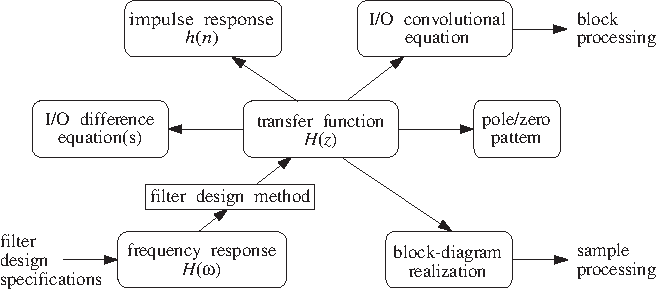
\includegraphics[width = 1\textwidth]{pic/transFunc.pdf}	
	\end{minipage}\\[0.3cm]

	\subsection{IIR und FIR Filter-Übertragungsfunktionen}
		\begin{itemize}
		 \item IIR Filter können im allgemeinen Fall als gebrochen rationale Funktionen dargestellt werden.\\[0.2cm]
		 \textbf{IIR}$\qquad$\fcolorbox{CadetRed}{white}{$H(z) = \dfrac{N(z)}{D(z)} = \dfrac{b_0 + b_1\,z^{-1} + b_2\,z^{-2} + \dots + b_N\,z^{-N} }{1 + a_1\,z^{-1} + a_2\,z^{-2} + \dots + a_M\,z^{-M} }$}
		 \item Das FIR Filter ist ein Spezialfall des IIR Filters ($a_i = 0$).\\[0.2cm]
		 \textbf{FIR}$\qquad$\fcolorbox{CadetRed}{white}{$H(z) = N(z) = b_0 + b_1\,z^{-1} + b_2\,z^{-2} + \dots + b_N\,z^{-N} $}
		\end{itemize}$ $\\[-0.8cm]

	\subsection{Impulsantwort \bm{$h(n)$}}
		\fcolorbox{CadetRed}{white}{$H(z)\quad \xrightarrow{\;\;Z^{-1}\;\;}\quad h(n)$}$\qquad\qquad$
		\fcolorbox{CadetRed}{white}{$h(n)\quad \xrightarrow{\;\;Z\;\;}\quad H(z)$}\\
		
	\subsection{I/O Differenzengleichung}
		$H(z)$ umformen, dass es bruchfrei und wird und $H(z)$ alleine auf der linken Seite steht.\\[0.2cm]
		$H(z)=\dfrac{N(z)}{D(z)}\qquad\Rightarrow\qquad H(z)\cdot \underbrace{\left[1 + a_1\,z^{-1}+ a_2\,z^{-2}+ ... + a_M\,z^{-M}\right]}_{D(z)}=\underbrace{\left[b_0 + b_1\,z^{-1}+ b_2\,z^{-2}+ ... + b_N\,z^{-N}\right]}_{N(z)}$\\[0.2cm]
		\begin{center}
			\fcolorbox{CadetRed}{white}{$H(z)= \underbrace{\left[b_0 + b_1\,z^{-1}+ b_2\,z^{-2}+ ... + b_N\,z^{-N}\right]}_{N(z)} - H(z)\cdot\underbrace{\left[a_1\,z^{-1}+ a_2\,z^{-2}+ ... + a_M\,z^{-M}\right]}_{D(z)-1}$}\\[0.2cm] $\text{\textcolor{white}{$Z$}}\;\text{\huge$\downarrow$}\;Z$\\[0.2cm]
			\fcolorbox{CadetRed}{white}{$h(n) = \left[b_0\,\delta(n) + b_1\,\delta(n-1)+ b_2\,\delta(n-2)+ ... + b_N\,\delta(n-N)\right] - \left[a_1\,h(n-1) + a_2\,h(n-2)+ ... + a_M\,h(n-M)\right]$}\\[0.2cm]
			$\delta(n) = x(n)\;\;\text{\huge$\downarrow$}\;\;h(n) = y(n)$\\[0.2cm]
			\fcolorbox{CadetRed}{white}{$y(n) = \left[b_0\,x(n) + b_1\,x(n-1)+ b_2\,x(n-2)+ ... + b_N\,x(n-N)\right] - \left[a_1\,y(n-1) + a_2\,y(n-2)+ ... + a_M\,y(n-M)\right]$}
		\end{center}$ $\\[-0.7cm]
\newpage
	\subsection{Frequenzgang \bm{$H(\omega)$}}
		In der Übertragungsfunktion $z$ durch $\e^{j\omega}$ ersetzen\\[0.2cm]
		\fcolorbox{CadetRed}{white}{$z = \e^{j\omega}$}$\qquad\rightarrow\qquad$
		\fcolorbox{CadetRed}{white}{$H(\omega) = H(z)|_{z = \e^{j\omega}} = \dfrac{b_0 + b_1\,\e^{-j\omega} + b_2\,\e^{-j\omega 2} + \dots + b_N\,\e^{-j\omega N} }{1 + a_1\,\e^{-j\omega} + a_2\,\e^{-j\omega 2} + \dots + a_M\,\e^{-j\omega M }}$}\\[0.2cm]
		Für den Betrag der Übertragungsfunktion $|H(\omega)|$ können Terme der Form $|1-a\,\e^{-j\omega}|$ noch vereinfacht werden.\\[0.2cm]
		\fcolorbox{CadetRed}{white}{$|1-a\,\e^{-j\omega}| = \sqrt{1-2a\cos(\omega)+a^2}$}\\[0.2cm]
		$|H(\omega)| = \dfrac{|1-z_1\,\e^{-j\omega}|\,|1-z_2\,\e^{-j\omega}|\,\dots\,|1-z_N\,\e^{-j\omega}|}{|1-p_1\,\e^{-j\omega}|\,|1-p_2\,\e^{-j\omega}|\,\dots\,|1-p_M\,\e^{-j\omega}|} = \dfrac{\sqrt{1-2z_1\cos(\omega)+z_1^2}\,\dots\,\sqrt{1-2z_N\cos(\omega)+z_N^2}}{\sqrt{1-2p_1\cos(\omega)+p_1^2}\,\dots\,\sqrt{1-2p_M\cos(\omega)+p_M^2}}$

	\subsection{Pol/Nullstellen - Diagramm}
		\begin{itemize}
		 \item Die Pole (Nullstellen von $D(z)$) und Nullstellen (Nullstellen von $N(z)$) können in der z-Ebene eingezeichnet werden.
		 \item Der Frequenzgang kann aus dem Pol/Nullstellen - Diagramm sehr einfach gezeichnet werden, indem ein man sich einen Punkt vorstellt, der von $0$ bis $\pi$ auf dem Einheitskreis wandert.
		 \subitem - Punkt fährt nahe am Pol vorbei $\quad\rightarrow\quad$ Frequenzgang wird gross.
		 \subitem - Punkt fährt nahe an Nullstelle vorbei $\quad\rightarrow\quad$ Frequenzgang wird klein.
		\end{itemize}
		\begin{minipage}{0.05\textwidth}$ $\end{minipage}
		\begin{minipage}{0.3\textwidth}
			\begin{tikzpicture}[>=latex', scale=1.4]
				\def\s{3};
				\def\f{1.3};
				\def\r{0.7};
				\def\a{60};
				\def\roc{0.9};

				\coordinate (c1) at (0,0);
	% 			\draw[line width=0.75,fill=CadetRed, opacity=0.5](c1)++(-\s/2,-\s/2)--++(\s,0)--++(0,\s)--++(-\s,0)--cycle ;
				\draw[line width=0.75](c1)++(-\s/2,-\s/2)node[above right]{kausal}--++(\s,0)--++(0,\s)node[below left]{$z$-Plane}--++(-\s,0)--cycle node[below right, CadetRed]{\textbf{ }};

	% 			\draw[line width=0.75,fill=white](c1)--++(-\f,0)--++(2*\f,0)--++(-\f,0)--++(0,-\f)--++(0,2*\f)--++(0,-\f)circle(\r);
				\draw[line width=0.75](c1)--++(-\f,0)--++(2*\f,0)--++(-\f,0)--++(0,-\f)--++(0,2*\f)--++(0,-\f)circle(0);

				\draw[line width=0.75,dashed](c1)--++(-\f,0)--++(2*\f,0)--++(-\f,0)--++(0,-\f)--++(0,2*\f)--++(0,-\f)circle(\roc);

				\draw[line width=0.75](c1)++(\roc,0.1)--++(0,-0.2)node[below right=-3pt,yshift=2pt]{1};


				\draw[line width=0.75,CadetRed,->](c1)++(0.4,0)arc(0:\a:0.4)node[yshift=-10pt,xshift=1pt]{\footnotesize$\omega$};

				\draw[line width=0.75,CadetRed,->](c1)--++({\roc*cos(\a)},{\roc*sin(\a)})--++({0.5*\roc*cos(90+\a)},{0.5*\roc*sin(90+\a)});
				\draw[line width=0.75,fill,CadetRed,->](c1)++({\roc*cos(\a)},{\roc*sin(\a)})circle(\r/15)node[above right=-1pt]{$\e^{j\omega}$};

				\draw[line width=0.75,fill,](c1)++(0.67,0.2)circle(\r/15)node[above left=-2pt,black]{$p_2$};
				\draw[line width=0.75,fill,](c1)++(0.67,-0.2)circle(\r/15)node[below left=-2pt,black]{$p_1$};
				\draw[line width=0.75,fill=white](c1)++(-\roc,0)circle(\r/15)node[above left=-1pt,black]{$z_1$};

				\draw[line width=0.75,fill=white](c1)++(-0.4,0.4)circle(\r/15)node[ right,black]{$z_2$};
				\draw[line width=0.75,fill=white](c1)++(-0.4,-0.4)circle(\r/15)node[right,black]{$z_3$};

			\end{tikzpicture}
		\end{minipage}
		\begin{minipage}{0.5\textwidth}
			\begin{tikzpicture}[>=latex', scale=1.4]
				\draw[->][line width=0.75](0,-0.2)--(0,2.8)node[right]{\footnotesize$|H(\omega)|$};
				\draw[->][line width=0.75](-0.2,0)--(3.6,0)node[below]{\footnotesize$\omega$};
				\draw[line width=0.75](-0,0.2)--(-0,-0.2)node[below]{$0$};
				\draw[line width=0.75](pi,0.2)--(pi,-0.2)node[below]{$\pi$};

				\draw[black, smooth,samples=100,domain=0:pi, line width=1,CadetRed]plot (\x,{0.12*(2.23607*sqrt(cos(\x*180/pi)+1)*sqrt(cos(\x*180/pi)+sin(\x*180/pi)+1.5)*sqrt(cos(\x*180/pi)-sin(\x*180/pi)+1.5))/(sqrt(-4*(cos(\x*180/pi)-0.25*sin(\x*180/pi)-0.25*4.2))*sqrt(-4*(4*cos(\x*180/pi)+sin(\x*180/pi)-4.2)))})node[above] {\footnotesize$ $};
			\end{tikzpicture}
		\end{minipage}

	\subsection{Realisation mit Blockdiagrammen}
		Es werden vier Arten von Blockdiagrammen unterschieden\\[0.2cm]
		\begin{minipage}{0.5\textwidth}
			\begin{itemize}
			\item Direktform (Siehe Seite 217)
			\item Parallelform (Siehe Seite 219)
			\end{itemize}
		\end{minipage}
		\begin{minipage}{0.5\textwidth}
			\begin{itemize}
			\item Kanonische Form (Siehe Seite 221)
			\item Transpolierte Form (Siehe Seite 222)
			\end{itemize}
		\end{minipage}$ $\\[-0.2cm]

		\textbf{Direktform}\\
		Aus der I/O Differenzengleichung kann direkt das Blockdiagramm der Direktform aufgezeichnet werden. Der Nachteil an dieser Variante ist, dass sehr viele Zustände gespeichert werden müssen.\\[0.2cm]
		\begin{tikzpicture}[>=latex', scale=1.1]
			\def\s{0.3};
			\def\l{1};
			\def\r{0.17};
			\def\dis{0.8};

			\coordinate (h1) at (0,0);
			\draw[line width=1,->](h1)++(0,-0.675)node[above right]{\footnotesize$x(n)$}--++(3.5-\r,0);
			\draw[line width=1,->](h1)++(3.5+\r,-0.675)--++(3.5-\r,0)node[above left]{\footnotesize$y(n)$};

			\foreach \i in {2,4,7}
			{
				\coordinate (h1) at (1,-\i/1.5);
				\draw[line width=1,fill=white](h1)++(-\s,-\s)--++(2*\s,0)--++(0,2*\s)--++(-2*\s,0)--cycle node at(h1)[xshift=0pt]{\footnotesize$z^{-1}$};
				\draw[line width=1,->](h1)++(0,0.675)--++(0,-0.38);
				\draw[line width=1,->](h1)++(0,-0.3)--++(0,-0.365)--++(2.5-\r,0);

				\coordinate (h1) at (6,-\i/1.5);
				\draw[line width=1,fill=white](h1)++(-\s,-\s)--++(2*\s,0)--++(0,2*\s)--++(-2*\s,0)--cycle node at(h1)[xshift=0pt]{\footnotesize$z^{-1}$};
				\draw[line width=1,->](h1)++(0,0.675)--++(0,-0.38);
				\draw[line width=1,->](h1)++(0,-0.3)--++(0,-0.365)--++(-2.5+\r,0);
			}

			\foreach \i in {2,4,6,9}
			{
				\coordinate (h1) at (2,{-(-1+\i)/1.5});
				\draw[line width=1,fill=white](h1)++(0,0)--++(0,1.2*\s)--++(2.2*\s,-1.2*\s)--++(-2.2*\s,-1.2*\s)--cycle;
			}

			\foreach \i in {4,6,9}
			{
				\coordinate (h1) at (5,{-(-1+\i)/1.5});
				\draw[line width=1,fill=white](h1)++(0,0)--++(0,1.2*\s)--++(-2.2*\s,-1.2*\s)--++(2.2*\s,-1.2*\s)--cycle;
			}

			\foreach \i in {2,4,6,9}
			{
				\coordinate (h1) at (3.5,{-(-1+\i)/1.5});
				\draw[line width=1,fill=white](h1)circle(\r)node{\Large$+$};
			}

			\foreach \i in {2,4,6,9}
			{
				\coordinate (h1) at (3.5,{-(-1+\i)/1.5});
				\draw[line width=1,fill=white](h1)circle(\r)node{\Large$+$};
			}
			\foreach \i in {4,6}
			{
				\coordinate (h1) at (3.5,{-(-1+\i)/1.5});
				\draw[line width=1](h1)++(0,\r)--++(0,0.5);
			}
			\coordinate (h1) at (3.5,{-(-1+9)/1.5});
			\draw[line width=1,->](h1)++(0,\r)--++(0,0.5)node[above=2pt]{$\vdots$};
			\foreach \i in {2,4,6}
			{
				\coordinate (h1) at (3.5,{-(-1+\i)/1.5});
				\draw[line width=1,->](h1)++(0,-0.5-\r)--++(0,0.5);
			}

			% x verzoegerungen
			\coordinate (h1) at (1,-4/1.5);
			\draw[line width=1](h1)++(0,0.675)node[left]{\footnotesize$x(n-1)$};
			\coordinate (h1) at (1,-6/1.5);
			\draw[line width=1,->](h1)++(0,0.675)node[left]{\footnotesize$x(n-2)$}--++(0,-0.3)node[yshift=-2.5pt]{$\vdots$};
			\coordinate (h1) at (1,-9/1.5);
			\draw[line width=1](h1)++(0,0.675)node[left]{\footnotesize$x(n-N)$};

			% y verzoegerungen
			\coordinate (h1) at (6,-4/1.5);
			\draw[line width=1](h1)++(0,0.675)node[right]{\footnotesize$y(n-1)$};
			\coordinate (h1) at (6,-6/1.5);
			\draw[line width=1,->](h1)++(0,0.675)node[right]{\footnotesize$y(n-2)$}--++(0,-0.3)node[yshift=-2.5pt]{$\vdots$};
			\coordinate (h1) at (6,-9/1.5);
			\draw[line width=1](h1)++(0,0.675)node[right]{\footnotesize$y(n-M)$};

			% B-Koeffizienten
			\coordinate (h1) at (2,{-(-1+2)/1.5});
			\draw[line width=1,fill=white](h1)node[right=-1pt]{\footnotesize$b_0$};
			\coordinate (h1) at (2,{-(-1+4)/1.5});
			\draw[line width=1,fill=white](h1)node[right=-1pt]{\footnotesize$b_1$};
			\coordinate (h1) at (2,{-(-1+6)/1.5});
			\draw[line width=1,fill=white](h1)node[right=-1pt]{\footnotesize$b_2$};
			\coordinate (h1) at (2,{-(-1+9)/1.5});
			\draw[line width=1,fill=white](h1)node[right=-1pt]{\footnotesize$b_N$};

			% A-Koeffizienten
			\coordinate (h1) at (5,{-(-1+4)/1.5});
			\draw[line width=1,fill=white](h1)node[left=-3pt]{\footnotesize-$a_1$};
			\coordinate (h1) at (5,{-(-1+6)/1.5});
			\draw[line width=1,fill=white](h1)node[left=-3pt]{\footnotesize-$a_2$};
			\coordinate (h1) at (5,{-(-1+9)/1.5});
			\draw[line width=1,fill=white](h1)node[left=-4pt]{\footnotesize-$a_M$};

		\end{tikzpicture}
		
		\textbf{Kanonische Form}\\
		Die Kanonische Form kann aus der Direktform abgeleitet werden. Dazu muss die rechte und linke Seite des Blockdiagrammes getauscht werden. Der Vorteil an dieser Variante ist, dass viel weniger Zustände gespeichert werden müssen.\\[0.2cm]
		\begin{tikzpicture}[>=latex', scale=1.1]
			\def\s{0.3};
			\def\l{1};
			\def\r{0.17};
			\def\dis{0.8};

			\coordinate (h1) at (0,0);
			\draw[line width=1,->](h1)++(0,-0.675)node[above right]{\footnotesize$x(n)$}--++(1-\r,0);
			\draw[line width=1,->](h1)++(1+\r,-0.675)--++(5-2*\r,0);
			\draw[line width=1,->](h1)++(3.5+\r,-0.675)--++(3.5-\r,0)node[above left]{\footnotesize$y(n)$};
			
			%verzoegerer
			\foreach \i in {2,4}
			{
				\coordinate (h1) at (3.5,-\i/1.5);
				\draw[line width=1,fill=white](h1)++(-\s,-\s)--++(2*\s,0)--++(0,2*\s)--++(-2*\s,0)--cycle node at(h1)[xshift=0pt]{\footnotesize$z^{-1}$};
				\draw[line width=1,->](h1)++(0,0.675)--++(0,-0.38);
				\draw[line width=1,->](h1)++(0,-0.3)--++(0,-0.365)--++(2.5-\r,0);
				\draw[line width=1,->](h1)++(0,-0.3)--++(0,-0.365)--++(-2.5+\r,0);
			}
			\coordinate (h1) at (3.5,-7/1.5);
			\draw[line width=1,fill=white](h1)++(-\s,-\s)--++(2*\s,0)--++(0,2*\s)--++(-2*\s,0)--cycle node at(h1)[xshift=0pt]{\footnotesize$z^{-1}$};
			\draw[line width=1,->](h1)++(0,0.675)--++(0,-0.38);
			\draw[line width=1](h1)++(0,-0.3)--++(0,-0.365)--++(2.5,0)--++(0,0.5);
			\draw[line width=1](h1)++(0,-0.3)--++(0,-0.365)--++(-2.5,0)--++(0,0.5);


		% 	% verstaerker rechts
			\foreach \i in {2,4,6,9}
			{
				\coordinate (h1) at (4.75,{-(-1+\i)/1.5});
				\draw[line width=1,fill=white](h1)++(0,0)--++(0,1.2*\s)--++(2.2*\s,-1.2*\s)--++(-2.2*\s,-1.2*\s)--cycle;
			}

			% verstaerker links
			\foreach \i in {4,6,9}
			{
				\coordinate (h1) at (2.25,{-(-1+\i)/1.5});
				\draw[line width=1,fill=white](h1)++(0,0)--++(0,1.2*\s)--++(-2.2*\s,-1.2*\s)--++(2.2*\s,-1.2*\s)--cycle;

			}

			% Addierer rechts
			\foreach \i in {2,4,6}
			{
				\coordinate (h1) at (6,{-(-1+\i)/1.5});
				\draw[line width=1,fill=white](h1)circle(\r)node{\Large$+$};
			}
			\foreach \i in {4,6}
			{
				\coordinate (h1) at (6,{-(-1+\i)/1.5});
				\draw[line width=1](h1)++(0,\r)--++(0,0.5);
			}
			\coordinate (h1) at (6,{-(-1+9)/1.5});
			\draw[line width=1,->](h1)++(0,\r)--++(0,0.5)node[above=2pt]{$\vdots$};
			\foreach \i in {2,4,6}
			{
				\coordinate (h1) at (6,{-(-1+\i)/1.5});
				\draw[line width=1,->](h1)++(0,-0.5-\r)--++(0,0.5);
			}
			% Addierer links
			\foreach \i in {2,4,6}
			{
				\coordinate (h1) at (1,{-(-1+\i)/1.5});
				\draw[line width=1,fill=white](h1)circle(\r)node{\Large$+$};
			}
			\foreach \i in {4,6}
			{
				\coordinate (h1) at (1,{-(-1+\i)/1.5});
				\draw[line width=1](h1)++(0,\r)--++(0,0.5);
			}
			\coordinate (h1) at (1,{-(-1+9)/1.5});
			\draw[line width=1,->](h1)++(0,\r)--++(0,0.5)node[above=2pt]{$\vdots$};
			\foreach \i in {2,4,6}
			{
				\coordinate (h1) at (1,{-(-1+\i)/1.5});
				\draw[line width=1,->](h1)++(0,-0.5-\r)--++(0,0.5);
			}

			% x verzoegerungen
			\coordinate (h1) at (3.5,-4/1.5);
			\draw[line width=1](h1)++(0,0.675)node[above left=-3pt]{\footnotesize$w(n-1)$};
			\coordinate (h1) at (3.5,-6/1.5);
			\draw[line width=1,->](h1)++(0,0.675)node[above left=-3pt]{\footnotesize$w(n-2)$}--++(0,-0.3)node[yshift=-2.5pt]{$\vdots$};

			% B-Koeffizienten
			\coordinate (h1) at (4.75,{-(-1+2)/1.5});
			\draw[line width=1,fill=white](h1)node[right=-1pt]{\footnotesize$b_0$};
			\coordinate (h1) at (4.75,{-(-1+4)/1.5});
			\draw[line width=1,fill=white](h1)node[right=-1pt]{\footnotesize$b_1$};
			\coordinate (h1) at (4.75,{-(-1+6)/1.5});
			\draw[line width=1,fill=white](h1)node[right=-1pt]{\footnotesize$b_2$};
			\coordinate (h1) at (4.75,{-(-1+9)/1.5});
			\draw[line width=1,fill=white](h1)node[right=-1pt]{\footnotesize$b_N$};

			% A-Koeffizienten
			\coordinate (h1) at (2.25,{-(-1+4)/1.5});
			\draw[line width=1,fill=white](h1)node[left=-3pt]{\footnotesize-$a_1$};
			\coordinate (h1) at (2.25,{-(-1+6)/1.5});
			\draw[line width=1,fill=white](h1)node[left=-3pt]{\footnotesize-$a_2$};
			\coordinate (h1) at (2.25,{-(-1+9)/1.5});
			\draw[line width=1,fill=white](h1)node[left=-4pt]{\footnotesize-$a_M$};

		\end{tikzpicture}

		\textbf{Transpolierte Form}\\
		Die Transpolierte Form kann aus der Kanonischen Form abgeleitet werden. Dazu muss das Blockdiagramm transponiert werden, d.h. Addierer mit Knoten und Knoten mit Addierer ersetzen, alle Flussrichtungen umkehren und Ein- und Ausgang vertauschen.\\[0.2cm]
		\begin{tikzpicture}[>=latex', scale=1.1]
			\def\s{0.3};
			\def\l{1};
			\def\r{0.17};
			\def\dis{0.8};

			\coordinate (h1) at (0,0);
			\draw[line width=1,->](h1)++(0,-0.675)node[above right]{\footnotesize$x(n)$}--++(3.5-\r,0);
			\draw[line width=1,->](h1)++(3.5+\r,-0.675)--++(3.5-\r,0)node[above left]{\footnotesize$y(n)$};

			\foreach \i in {2,4,7}
			{
				\coordinate (h1) at (1,-\i/1.5);
				\draw[line width=1,->](h1)++(0,0.65)--++(0,-1.315)--++(2.5-\r,0);

				\coordinate (h1) at (6,-\i/1.5);
				\draw[line width=1,->](h1)++(0,0.65)--++(0,-1.315)--++(-2.5+\r,0);
			}

			\foreach \i in {2,4,6,9}
			{
				\coordinate (h1) at (1.75,{-(-1+\i)/1.5});
				\draw[line width=1,fill=white](h1)++(0,0)--++(0,1.2*\s)--++(2.2*\s,-1.2*\s)--++(-2.2*\s,-1.2*\s)--cycle;
			}

			\foreach \i in {4,6,9}
			{
				\coordinate (h1) at (5.25,{-(-1+\i)/1.5});
				\draw[line width=1,fill=white](h1)++(0,0)--++(0,1.2*\s)--++(-2.2*\s,-1.2*\s)--++(2.2*\s,-1.2*\s)--cycle;
			}

			\foreach \i in {2,4,6,9}
			{
				\coordinate (h1) at (3.5,{-(-1+\i)/1.5});
				\draw[line width=1,fill=white](h1)circle(\r)node{\Large$+$};
			}

			\foreach \i in {2,4,6,9}
			{
				\coordinate (h1) at (3.5,{-(-1+\i)/1.5});
				\draw[line width=1,fill=white](h1)circle(\r)node{\Large$+$};
			}
			\foreach \i in {4,6}
			{
				\coordinate (h1) at (3.5,{-(-1+\i)/1.5});
				\draw[line width=1](h1)++(0,\r)--++(0,0.5);
			}
			\coordinate (h1) at (3.5,{-(-1+9)/1.5});
			\draw[line width=1,->](h1)++(0,\r)--++(0,0.5)node[above=2pt]{$\vdots$};
			\foreach \i in {2,4,6}
			{
				\coordinate (h1) at (3.5,{-(-1+\i)/1.5});
				\draw[line width=1,->](h1)++(0,-0.5-\r)--++(0,0.5);
			}

			\foreach \i in {2,4}
			{
				\coordinate (h1) at (3.5,-\i/1.5-0.1);
				\draw[line width=1,fill=white](h1)++(-\s,-\s)--++(2*\s,0)--++(0,2*\s)--++(-2*\s,0)--cycle node at(h1)[xshift=0pt]{\footnotesize$z^{-1}$};
			}

			\coordinate (h1) at (6,-6/1.5);
			\draw[line width=1,->](h1)++(0,0.675)--++(0,-0.3)node[yshift=-3pt]{$\vdots$};
			\coordinate (h1) at (1,-6/1.5);
			\draw[line width=1,->](h1)++(0,0.675)--++(0,-0.3)node[yshift=-3pt]{$\vdots$}; 


			% verzoegerungen
			\coordinate (h1) at (3.5,-4/1.5);
			\draw[line width=1](h1)++(0,0.675)node[right, yshift=33pt]{\footnotesize$w(n-1)$};
			\coordinate (h1) at (3.5,-6/1.5);
			\draw[line width=1](h1)++(0,0.675)node[right, yshift=33pt]{\footnotesize$w(n-2)$};

			% B-Koeffizienten
			\coordinate (h1) at (1.75,{-(-1+2)/1.5});
			\draw[line width=1,fill=white](h1)node[right=-1pt]{\footnotesize$b_0$};
			\coordinate (h1) at (1.75,{-(-1+4)/1.5});
			\draw[line width=1,fill=white](h1)node[right=-1pt]{\footnotesize$b_1$};
			\coordinate (h1) at (1.75,{-(-1+6)/1.5});
			\draw[line width=1,fill=white](h1)node[right=-1pt]{\footnotesize$b_2$};
			\coordinate (h1) at (1.75,{-(-1+9)/1.5});
			\draw[line width=1,fill=white](h1)node[right=-1pt]{\footnotesize$b_N$};

			% A-Koeffizienten
			\coordinate (h1) at (5.25,{-(-1+4)/1.5});
			\draw[line width=1,fill=white](h1)node[left=-3pt]{\footnotesize-$a_1$};
			\coordinate (h1) at (5.25,{-(-1+6)/1.5});
			\draw[line width=1,fill=white](h1)node[left=-3pt]{\footnotesize-$a_2$};
			\coordinate (h1) at (5.25,{-(-1+9)/1.5});
			\draw[line width=1,fill=white](h1)node[left=-4pt]{\footnotesize-$a_M$};
		\end{tikzpicture}
		
\section{Systemantwort auf sinusförmiges Eingangssignal}
	Wenn in ein LTI-System ein sinusförmiges Eingangssignal gegeben wird, so wird auch ein sinusförmiges Ausgangssignal derselben Frequenz herauskommen.\\[0.2cm]
	\begin{minipage}{0.5\textwidth}
		\begin{tikzpicture}[>=latex', scale=1]
			\draw[<-,line width=1](-0.6,0)--(-3.2,0)node[above right]{$x(n)=\e^{j\omega_0n}$};
			\draw[->,line width=1](0.6,0)--(4.2,0)node[above left]{$y(n) = H(\omega_0)\,\e^{j\omega_0n}$};
			\draw[line width=1](-0.6,-0.6)--(-0.6,0.6)--node [above]{LTI}(0.6,0.6)--(0.6,-0.6)--(-0.6,-0.6)node at (0,0){$H$};
		\end{tikzpicture} 
	\end{minipage}
	\begin{minipage}{0.5\textwidth}
		\fcolorbox{CadetRed}{white}{$\begin{array}{lcl}\e^{j\omega_0n}&\quad\xrightarrow{\;\;H\;\;} &\quad H(\omega_0)\,\e^{j\omega_0n}\\\e^{j\omega_0n}&\quad\xrightarrow{\;\;H\;\;} &\quad |H(\omega_0)|\,\e^{j\omega_0n + jarg(H(\omega_0))} \end{array}\\  $}
	\end{minipage}\\[0.2cm]

	\begin{minipage}{0.55\textwidth}
	Ein LTI System:\\[-0.35cm]
		\begin{itemize}
		\item erzeugt keine neuen Frequenzen\\[-0.35cm]
		\item dämpft/verstärkt das Signal mit $|H(\omega_0)|$\\[-0.35cm]
		\item verzöger das Signal um $arg(H(\omega_0))$\\[-0.35cm]
		\item erscheint am Ausgang mit derselben Frequenz\\[0.2cm]
		\end{itemize}

		\fcolorbox{CadetRed}{white}{$\begin{array}{lcl}\cos(\omega_0n)&\quad\xrightarrow{\;\;H\;\;} &\quad |H(\omega_0)|\cdot\cos(\omega_0n + arg(H(\omega_0)))\\\sin(\omega_0n)&\quad\xrightarrow{\;\;H\;\;} &\quad |H(\omega_0)|\cdot\sin(\omega_0n + arg(H(\omega_0))) \end{array}\\  $}
	\end{minipage}
	\begin{minipage}{0.45\textwidth}
		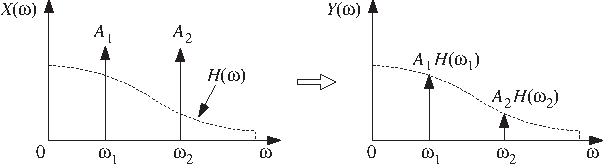
\includegraphics[width = 1\textwidth]{pic/frequenzgang.pdf}\\[1cm]
	\end{minipage}
\newpage
	\subsection{Phasen- und Gruppenverzögerung}
		\textbf{Phasenverzögerung}\\[0.1cm]
		Die Phasenverzögerung beschreibt, welche Frequenz um wie viele Samples verzögert wird. Die Anzahl verzögerter Samples muss nicht ganzzahlig sein.\\[0.2cm]
		\fcolorbox{CadetRed}{white}{$d(\omega) = -\dfrac{arg(H(\omega))}{\omega}$}$\qquad\rightarrow\quad \e^{j\omega n} \;\xrightarrow{\;H\;} \;|H(\omega)|\,\e^{j\omega (n-d(\omega))}$\\[0.3cm]
		Verzögert das Filter alle Frequenzen um die selbe Anzahl Samples, handelt es sich um ein linearphasiges Filter\\[0.2cm]
		\fcolorbox{CadetRed}{white}{$\text{linearphasiges Filter}\quad\Leftrightarrow\quad d(\omega) = D = \text{konstant}$}\\[0.2cm]
		$\rightarrow$ FIR Filter können sehr einfach als linearphasige Filter designed werden.\\[0.2cm]
		\textbf{Gruppenverzögerung}\\[0.2cm]
		\begin{minipage}{0.25\textwidth}
			\fcolorbox{CadetRed}{white}{$d_g(\omega) = -\dfrac{d\,arg(H(\omega))}{d\omega}$}
		\end{minipage}
		\begin{minipage}{0.75\textwidth}
			Wenn in einem Frequenzintervall alle Frequenzen dieselbe Phasenverzögerung haben, ist die Gruppenverzögerung eine Konstante.
		\end{minipage}

	\subsection{Einschwingvorgang}
		Wird eine Schwinung eingeschaltet, so braucht das Filter eine gewisse Zeit, bis es eingeschwungen ist\\ (im steady state).\\[0.2cm]
		\begin{tabularx}{0.9\textwidth}{p{3.1cm}cl}
			\textbf{Einschaltsignal:} && $x(n) = \e^{j\omega_0n}\,u(n)$\\[0.2cm]
			&& $X(z)=\dfrac{1}{1-\e^{j\omega_0}\,z^{-1}}\quad\qquad \text{ROC }|z|>1$\\[0.5cm]
		 \hline&&\\[-0.2cm]
			\textbf{Filter:} && $H(z)=\dfrac{N(z)}{D(z)} = \dfrac{N(z)}{(1-p_1\,z^{-1})\,(1-p_1\,z^{-1})\,\dots\,(1-p_M\,z^{-1})}$\\[0.5cm]
		\hline&&\\[-0.2cm]
			\textbf{Ausgangssignal:} && $Y(Z) = \dfrac{H(\omega_0)}{1-\e^{j\omega_0}\,z^{-1}}+\dfrac{B_1}{1-p_1\,z^{-1}}+\dfrac{B_2}{1-p_2\,z^{-1}}+\dots+\dfrac{B_M}{1-p_M\,z^{-1}}$\\[0.5cm]
			&& \fcolorbox{CadetRed}{white}{$y(n) = H(\omega_0)\,\e^{j\omega_0n} + \underbrace{B_1\,p_1^n+B_2\,p_2^n+\dots+B_M\,p_M^n}_{\text{Einschwingvorgang}}$}\\[0.9cm]
		\hline&&\\[-0.2cm]
			\textbf{Übergang in\newline Steady State}&&\fcolorbox{CadetRed}{white}{Alle Pole $|p_i|<1\qquad\Rightarrow\qquad \mylim{n\to\infty}{y(n)} = H(\omega_0)\,\e^{j\omega_0n}$}\\
		\end{tabularx}\\[0.2cm] 

		\textbf{Einschwingzeit:}\\[0.2cm]
			Der Pol am nächsten beim Einheitskreis dominiert die Zeitdauer des Einschwingvorganges\\[0.2cm]
			\fcolorbox{CadetRed}{white}{$\rho = \max\limits_{i}^{}\left\{|p_i|\right\}$} \\[0.2cm]
			Der Steady State gilt als erreicht, wenn der Beitrag des langsamste Pols unter 1\% gefallen ist.\\[0.2cm]
			\fcolorbox{CadetRed}{white}{$\rho^{n_{\text{eff}}} = \epsilon = 0.01$}$\qquad\Rightarrow\qquad$\textbf{Zeitkonstante des Filters:}$\qquad$\fcolorbox{CadetRed}{white}{$n_{\text{eff}} = \dfrac{\ln(\epsilon)}{\ln(\rho)} = \dfrac{\ln(1/\epsilon)}{\ln(1/\rho)}$}
			
	\subsection{DC-Gain und AC-Gain}
		Das Einschwingverhalten des Einheitssprunges $u(n)$ resultiert im DC-Gain\\[0.2cm]		\fcolorbox{CadetRed}{white}{$\mylim{n\to\infty}{y(n)} = \left.H(\omega_0)\,\e^{j\omega_0n}\right|_{\omega_0 = 0} = H(0)$}$\qquad\qquad\quad\qquad$\textbf{DC-Gain:}$\quad$\fcolorbox{CadetRed}{white}{$H(0) = \left.H(z)\right|_{z=1} = \mysum{n=0}{\infty}{h(n)}$}\\[0.2cm]
		Das Einschwingverhalten des alternierenden Einheitssprunges $(-1)^n\,u(n)$ resultiert im AC-Gain\\[0.2cm]
		\fcolorbox{CadetRed}{white}{$\mylim{n\to\infty}{y(n)} = \left.H(\omega_0)\,\e^{j\omega_0n}\right|_{\omega_0 = \pi} = H(\pi)\,(-1)^n$}$\qquad\qquad$\textbf{AC-Gain:}$\quad$\fcolorbox{CadetRed}{white}{$H(\pi) = \left.H(z)\right|_{z=-1} = \mysum{n=0}{\infty}{(-1)^n\,h(n)}$}
\newpage
	\subsection{Einschwingverhalten von Grenzstabilen Systemen}
		\begin{minipage}{0.75\textwidth}
			Wird an ein Grenzstabiles System, mit einem konjugiert komplexen Polpaar auf dem Einheitskreis, eine Einschaltschwinung angelegt, so resultiert folgende Ausgangsschwingung.\\[0.3cm]
			\fcolorbox{CadetRed}{white}{$y(n) = H(\omega_0)\,\e^{j\omega_0n} +\underbrace{ B_1\,p_1^n+B_1^\ast\,p_1^{\ast n}}_{\text{grenzstabile Pole}}+\underbrace{B_2\,p_2^n+B_3\,p_3^n+\dots+B_M\,p_1^n}_{\text{Einschwingvorgang}}$}
		\end{minipage}\begin{minipage}{0.05\textwidth}$ $\end{minipage}
		\begin{minipage}{0.25\textwidth}
			\begin{tikzpicture}[>=latex', scale=1.2]
				\def\s{2.8};
				\def\f{1.2};
				\def\r{0.7};
				\def\a{60};
				\def\roc{0.9};
				
				\coordinate (c1) at (0,0);
				\draw[line width=0.75](c1)++(-\s/2,-\s/2)node[above right]{ }--++(\s,0)--++(0,\s)node[below left]{$z$-Plane}--++(-\s,0)--cycle node[below right, CadetRed]{\textbf{ }};
				\draw[line width=0.75](c1)--++(-\f,0)--++(2*\f,0)--++(-\f,0)--++(0,-\f)--++(0,2*\f)--++(0,-\f)circle(0);
				\draw[line width=0.75,dashed](c1)circle(\roc);
				\draw[line width=0.75](c1)++(\roc,0.1)--++(0,-0.2)node[below right=-3pt,yshift=2pt]{1};
				\draw[line width=0.75,fill,CadetRed](c1)++(0.75,0.5)circle(\r/15)node[below left=-2pt]{$p_1$};
				\draw[line width=0.75,fill,CadetRed](c1)++(0.75,-0.5)circle(\r/15)node[above left=-2pt]{$p_1^\ast$};
				\draw[line width=0.75,fill](c1)++(-0.6,0)circle(\r/15)node[above right=-1pt,black]{$p_2$};
				\draw[line width=0.75,fill](c1)++(-0.2,0.7)circle(\r/15)node[ below,black]{$p_3$};
				\draw[line width=0.75,fill](c1)++(-0.2,-0.7)circle(\r/15)node[above,black]{$p_4$};
			\end{tikzpicture}
		\end{minipage}
		Nach dem Übergang in den Steady State resultiert folgende Ausgangsschwingung:\\[0.2cm]
		\fcolorbox{CadetRed}{white}{$\mylim{n\to\infty}{y(n)} = H(\omega_0)\,\e^{j\omega_0n} +\underbrace{ B_1\,p_1^n+B_1^\ast\,p_1^{\ast n}}_{\text{grenzstabile Pole}} = H(\omega_0)\,\e^{j\omega_0n} +\underbrace{ B_1\,\e^{j\theta_1n}+B_1^\ast\,\e^{-j\theta_1n}}_{\text{Sinusschwingung}}$}
		\begin{itemize}
		 \item Das Ausgangsignal klingt nicht ab sondern schwingt.
		 \item Die Frequenz der Eingangsschwingung darf nicht dieselbe sein, wie die der Pole auf dem Eingheitskreis!
		 \item $\e^{j\omega_0n} = p_1 = \e^{j\theta_1n}\quad\Rightarrow\quad$ Doppelter Pol $\quad\Rightarrow\quad$ System ist in Resonanz, Ausgang wird immer grösser!
		\end{itemize}
		
	\subsection{Einschwingverhalten von FIR Filtern}
		Bei FIR Filtern ist der Steady State nach M Samples erreicht (siehe Kapitel \ref{Transienten und Steady-State})\\[-0.2cm]

\section{Pol/Nullstellen Filterdesign}
	Durch das Platzieren von Polen und Nullstellen können intuitive Filter designed werden. Durch die Pol-und Nullstellen ist alles, bis auf einen Verstärkungsfaktor, definiert.\\[-0.3cm]
	
	\subsection{Filter erster Ordnung}
		\vspace*{-0.6cm}\begin{minipage}{0.5\textwidth}
			\textbf{Allgemeine Form:}$\qquad$\fcolorbox{CadetRed}{white}{$H(z) = G\,\dfrac{1+b\,z^{-1}}{1-a\,z^{-1}}$}\\[0.2cm]
			mit $|a|<1$ und $|b|\leq1$
		\end{minipage}
		\begin{minipage}{0.5\textwidth}
			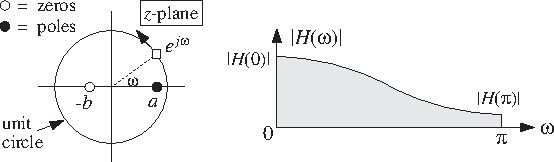
\includegraphics[width = 1\textwidth]{pic/firstOrderFilter.pdf}	
		\end{minipage}
		\textbf{Designparameter des Filters:}
		\begin{itemize}
			\item Steilheit (Stärke) des Filters$\quad\rightarrow\quad$Verhältnis von AC- zu DC-Gain\\[0.2cm]
			\fcolorbox{CadetRed}{white}{$\dfrac{H(\pi)}{H(0)} =\dfrac{(1-b)\,(1-a)}{(1+b)\,(1+a)}\quad\Rightarrow\quad \dfrac{H(\pi)}{H(0)}\begin{cases}< 1 & \text{Tiefpassfilter}\\ >1  &\text{Hochpassfilter}\end{cases}$}
			\item Maximale Zeitkonstante (Einschwingzeit) von $N$ Samples\\[0.2cm]
			\fcolorbox{CadetRed}{white}{$n_{\text{eff}} = \dfrac{\ln(\epsilon)}{\ln(|a|)} \leq N$}
			\item Verstärkungsfaktor $G$ wird oft so gewählt, dass bei einem Tiefpassfilter $|H(0)|=1$ ist und bei einem Hochpassfilter $|H(\pi)|=1$ ist.
		\end{itemize}$ $\\[-1cm]

	\subsection{Resonator}
		Mittels eines konjugiert komplexen Polpaares nahe am Einheitskreis kann ein Resonator gebaut werden. Dabei gelten folgende grundlegenden Zusammenhänge:\\[0.2cm]
		\fcolorbox{CadetRed}{white}{Schmalere Bandbreite$\quad\Leftrightarrow\quad$ Pole näher am Einheitskreis$\quad\Leftrightarrow\quad$ Längere Einschwingzeit des Filters }\\[0.3cm]
		\textbf{Allgemeine Form:}$\qquad$\\[0.2cm]
		\fcolorbox{CadetRed}{white}{$H(z) = \dfrac{G}{(1-R\,\e^{j\omega_0}\,z^{-1})\,(1-R\,\e^{-j\omega_0}\,z^{-1})} = \dfrac{G}{(1 + a_1\,z^{-1}+a_2\,z^{-2}})$}$\qquad$mit $\;\; p = R\,\e^{j\omega_0}$ und $|R|\leq 1$\\[0.2cm]
		\fcolorbox{black}{white}{$a_1 = -2R\cos(\omega_0)\qquad a_2 = R^2$}$\qquad$
		\fcolorbox{black}{white}{$|H(\omega_0)| = 1\quad\Rightarrow\quad G = (1-R)\,\sqrt{1-2R\cos(2\omega_0)+R^2}$}\\
		\begin{minipage}{0.47\textwidth}
			\textbf{Bandbreite als Designparameter:}\\[0.2cm]
			Die $3\db$ Bandbreite ist die Breite auf der halben maximalen Höhe des quadrierten Frequenzganges.\\[0.2cm]
			\text{\textcolor{white}{$\Rightarrow\quad$}}\fcolorbox{CadetRed}{white}{$\Delta\omega = \omega_2-\omega_1$}$\qquad$
			\fcolorbox{CadetRed}{white}{$|H(\omega_{1,2})|^2 = \dfrac{|H(\omega_0)|^2}{2}$}\\[0.2cm]$\quad\Rightarrow\quad$\fcolorbox{CadetRed}{white}{$10\log\left(\dfrac{|H(\omega_{1,2})|^2}{|H(\omega_0)|^2}\right) = 10\log\left(\dfrac{1}{2}\right)=-3\db$}
		\end{minipage}\begin{minipage}{0.03\textwidth}$ $\end{minipage}
		\begin{minipage}{0.55\textwidth}
			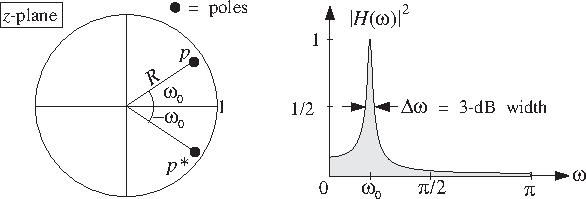
\includegraphics[width = 0.9\textwidth]{pic/resonator.pdf}\\[0.2cm]
			Ist der Pol nahe am Einheitskreis gilt:$\quad$
			\fcolorbox{CadetRed}{white}{$\Delta\omega\approx 2(1-R)$}
		\end{minipage}\\[0.2cm]
		
	\subsection{Notch- und Comb-Filter}
		\begin{minipage}{0.47\textwidth}
			Durch das ''Hintereinanderlegen'' von Polen $(p = R\,\e^{j\omega_0})$ und Nullstellen $(z = r\,\e^{j\omega_0})$ können gezielt bestimmte Frequenzen verstärkt bzw. unterdrückt werden.\\[-0.3cm]
			\begin{itemize}
			\item Pol näher am Einheitskreis ($R>r$)\\
			\text{$\;\Rightarrow\quad$} Verstärkung dieser Frequenz (Comb)\\[-0.3cm]
			\item Nullstelle näher am Einheitskreis ($R<r$)\\
			\text{$\;\Rightarrow\quad$} Unterdrückung dieser Frequenz (Notch)\\[-0.3cm]
			\end{itemize}
		\end{minipage}\begin{minipage}{0.03\textwidth}$ $\end{minipage}
		\begin{minipage}{0.5\textwidth}
			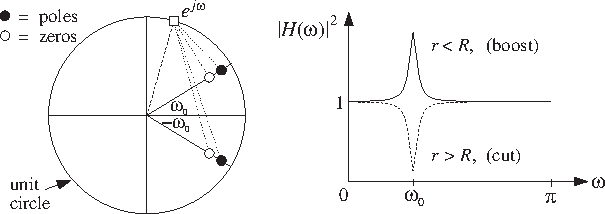
\includegraphics[width = 1\textwidth]{pic/notch.pdf}	
		\end{minipage}\\[0.2cm]
		\textbf{Allgemeine Form:}$\qquad$
		\fcolorbox{CadetRed}{white}{$H(z)= \dfrac{N(z)}{D(z)} = \dfrac{\myprod{i=1}{N}{(1-r\,\e^{j\omega_i}\,z^{-1})}}{\myprod{i=1}{N}{(1-R\,\e^{j\omega_i}\,z^{-1})}}$}$\qquad\quad\begin{array}{l}R<r\quad \rightarrow\quad\text{Notchfilter}\\R>r\quad \rightarrow\quad\text{Combfilter}\\[0.2cm]
		|R|<1\;\;\cap\;\;|r|\leq1\end{array}$\\[0.2cm]

	\subsection{Inverse Filterung}
		\begin{minipage}{0.47\textwidth}
			Oft ist gefordert, eine bestimmte Filterung rückgängig zu machen (z.B. Kanalausgleichung). Dazu kann grundsätzlich die Inverse Filterfunktion verwendet werden.\\[0.2cm]
			\textbf{Inversefilter:}$\qquad$\fcolorbox{CadetRed}{white}{$H_\text{inv}(z) = \dfrac{1}{H(z)}$}
		\end{minipage}\begin{minipage}{0.03\textwidth}$ $\end{minipage}
		\begin{minipage}{0.5\textwidth}
			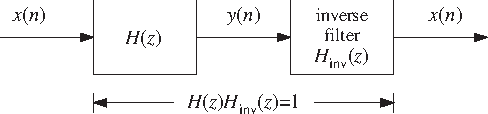
\includegraphics[width = 1\textwidth]{pic/invFiltering.pdf}	
		\end{minipage}\\
		
		Die Inversefilterung hat jedoch zwei bedeutende Probleme:\\[-0.6cm]
		\begin{itemize}
		 \item Das Rauschen wird auch inverse gefiltert.\\[-0.7cm]
		 \item Das Inversefilter muss stabil sein.
		\end{itemize}
		\begin{description}
		 \item [Rauschen:] $ $\newline Wird das verrauschte Signal inverse gefiltert, so wird das Rauschen in den Frequenzbereichen stark verstärkt, in denen das ursprüngliche Filter stark dämpfte $\quad\rightarrow\quad$ Verschlechterung der SNR!\\[0.2cm]
		 \fcolorbox{CadetRed}{white}{$Y(z) = H(z)\cdot X(z) + N(z)\qquad\Rightarrow\quad \hat X(z) = H_\text{inv}(z)\cdot Y(z) = X(z) + \dfrac{N(z)}{H(z)}$}
		 \item [Stabilität des Inversefilters:] $ $\newline
			Ist das ursprüngliche, kausale Filter $H(z)$ stabil (alle Pole innerhalb des Einheitskreises) so heisst dies nicht das das inverse Filter $H_\text{inv}(z)$ auch stabil ist. Durch die Invertierung werden alle Pole zu Nullstellen und alle Nullstellen zu Polen. Dies bedeutet, das Nullstellen, die vorher ausserhalb des Einheiskreises lagen zu Polen werden und das Filter im kausalen Fall dadruch instabil wird. Die Lösung dafür lautet, dass in diesem Fall die akausale Impulsantwort des Inversfilters genommen wird, diese um D Samples verzögert und wenn sie genügend abgeklungen ist (nach D Samples) einfach abgeschnitten wird. Mit dieser Lösung ist das Filter jedoch nur noch eine Approximation des eigentlichen Inversefilters.
		\end{description}

\chapter{Realisierung digitaler Filter \textcolor{black}{\small S.265}}
% 
% (c) Copyright 2016 Tabea Mendez
% 
% This source is free: you can redistribute it and/or modify
% it under the terms of the GNU General Public License as published by
% the Free Software Foundation, either version 3 of the License, or
% (at your option) any later version.
% 
% This source is distributed in the hope that it will be useful,
% but WITHOUT ANY WARRANTY; without even the implied warranty of
% MERCHANTABILITY or FITNESS FOR A PARTICULAR PURPOSE.  See the
% GNU General Public License for more details.
% 
% You should have received a copy of the GNU General Public License
% along with this source.  If not, see <http://www.gnu.org/licenses/>.
%
%%%%%%%%%%%%%%%%%%%%%%%%%%%%%%%%%%%%%%%%%%%%%%%%%%%%%%%%%%%%%%%%%%%%%%%%%%%%%%

\section{Direktform}  
	\begin{itemize}
	 \item Blockdiagramm kann direkt aus der I/O Differenzengleichung aufgezeichnet werden.\\[-0.6cm]
 	 \item Es sind sehr viele Speicherstellen notwendig.\\[-0.6cm]
	 \item Innere Zustände ($v_i,w_i$) definieren, damit der Ausgang aus dem aktuellen Eingang und den Zuständen berechnet werden kann. \\[-0.6cm]
	 \item Innere Zustände mit Null initialisieren $v_i = 0$ und $w_i = 0$
	\end{itemize}
	\begin{minipage}{0.57\textwidth}
		\textbf{Übertragungsfunktion}\\[0.2cm]
		\fcolorbox{CadetRed}{white}{$H(z) = \dfrac{N(z)}{D(z)} = \dfrac{b_0 + b_1\,z^{-1} + b_2\,z^{-2} + \dots + b_N\,z^{-N} }{1 + a_1\,z^{-1} + a_2\,z^{-2} + \dots + a_M\,z^{-M} }$}\\[0.4cm]
		\textbf{I/O Differenzengleichung}\\[0.2cm]
		\fcolorbox{CadetRed}{white}{$\begin{array}{ll}y(n)=&\;\big[b_0\,x(n) + b_1\,x(n-1)+ ... + b_N\,x(n-N)\big]\\[0.15cm] &\!\!\! - \big[a_1\,y(n-1)+ ... + a_M\,y(n-M)\big]\end{array}$}\\[0.4cm]
		\textbf{Algorithmus}\\[0.2cm]
		\begin{tabular}{|lclll|}
		 \hline &&&&$ $\\[-0.3cm]
		 \multicolumn{5}{|l|}{for each input $x$ do:}\\
		  &$v_0$&$ =$& $x$&\\
		  &$w_0$&$ = $&\multicolumn{2}{l|}{$b_0v_0 + b_1v_1 + \hdots + b_Nv_N - a_1w_1- \hdots  - a_Mw_M$}\\
		  &$y$&$ =$&$ w_0$&\\
		  &$v_i$&$ =$&$ v_{i-1}$ & $\qquad \quad i = N,N-1,\hdots,1$\\
		  &$w_i$& $=$&$ w_{i-1}$ & $\qquad \quad i = M,M-1,\hdots,1$\\[0.1cm]
		 \hline
		\end{tabular}
	\end{minipage}
	\begin{minipage}{0.43\textwidth}
		\begin{danger}
		$v_0$ und $w_0$ sind keine Zustände, sondern Ein- und Ausgangssignal.
		\end{danger}$ $\\
		
		\begin{tikzpicture}[>=latex', scale=1.1]
			\def\s{0.3};
			\def\l{1};
			\def\r{0.17};
			\def\dis{0.8};

			\coordinate (h1) at (0,0);
			\draw[line width=1,->](h1)++(0,-0.675)node[above right]{\footnotesize$x(n)=v_0$}--++(3.5-\r,0);
			\draw[line width=1,->](h1)++(3.5+\r,-0.675)--++(3.5-\r,0)node[above left]{\footnotesize$w_0=y(n)$};

			\foreach \i in {2,4,7}
			{
				\coordinate (h1) at (1,-\i/1.5);
				\draw[line width=1,fill=white](h1)++(-\s,-\s)--++(2*\s,0)--++(0,2*\s)--++(-2*\s,0)--cycle node at(h1)[xshift=0pt]{\footnotesize$z^{-1}$};
				\draw[line width=1,->](h1)++(0,0.675)--++(0,-0.38);
				\draw[line width=1,->](h1)++(0,-0.3)--++(0,-0.365)--++(2.5-\r,0);

				\coordinate (h1) at (6,-\i/1.5);
				\draw[line width=1,fill=white](h1)++(-\s,-\s)--++(2*\s,0)--++(0,2*\s)--++(-2*\s,0)--cycle node at(h1)[xshift=0pt]{\footnotesize$z^{-1}$};
				\draw[line width=1,->](h1)++(0,0.675)--++(0,-0.38);
				\draw[line width=1,->](h1)++(0,-0.3)--++(0,-0.365)--++(-2.5+\r,0);
			}

			\foreach \i in {2,4,6,9}
			{
				\coordinate (h1) at (2,{-(-1+\i)/1.5});
				\draw[line width=1,fill=white](h1)++(0,0)--++(0,1.2*\s)--++(2.2*\s,-1.2*\s)--++(-2.2*\s,-1.2*\s)--cycle;
			}

			\foreach \i in {4,6,9}
			{
				\coordinate (h1) at (5,{-(-1+\i)/1.5});
				\draw[line width=1,fill=white](h1)++(0,0)--++(0,1.2*\s)--++(-2.2*\s,-1.2*\s)--++(2.2*\s,-1.2*\s)--cycle;
			}

			\foreach \i in {2,4,6,9}
			{
				\coordinate (h1) at (3.5,{-(-1+\i)/1.5});
				\draw[line width=1,fill=white](h1)circle(\r)node{\Large$+$};
			}

			\foreach \i in {2,4,6,9}
			{
				\coordinate (h1) at (3.5,{-(-1+\i)/1.5});
				\draw[line width=1,fill=white](h1)circle(\r)node{\Large$+$};
			}
			\foreach \i in {4,6}
			{
				\coordinate (h1) at (3.5,{-(-1+\i)/1.5});
				\draw[line width=1](h1)++(0,\r)--++(0,0.5);
			}
			\coordinate (h1) at (3.5,{-(-1+9)/1.5});
			\draw[line width=1,->](h1)++(0,\r)--++(0,0.5)node[above=2pt]{$\vdots$};
			\foreach \i in {2,4,6}
			{
				\coordinate (h1) at (3.5,{-(-1+\i)/1.5});
				\draw[line width=1,->](h1)++(0,-0.5-\r)--++(0,0.5);
			}

			% x verzoegerungen
			\coordinate (h1) at (1,-4/1.5);
			\draw[line width=1](h1)++(0,0.675)node[left=3pt]{\footnotesize$v_1$};
			\coordinate (h1) at (1,-6/1.5);
			\draw[line width=1,->](h1)++(0,0.675)node[left=3pt]{\footnotesize$v_2$}--++(0,-0.3)node[yshift=-2.5pt]{$\vdots$};
			\coordinate (h1) at (1,-9/1.5);
			\draw[line width=1](h1)++(0,0.675)node[left=3pt]{\footnotesize$v_N$};

			% y verzoegerungen
			\coordinate (h1) at (6,-4/1.5);
			\draw[line width=1](h1)++(0,0.675)node[right=3pt]{\footnotesize$w_1$};
			\coordinate (h1) at (6,-6/1.5);
			\draw[line width=1,->](h1)++(0,0.675)node[right=3pt]{\footnotesize$w_2$}--++(0,-0.3)node[yshift=-2.5pt]{$\vdots$};
			\coordinate (h1) at (6,-9/1.5);
			\draw[line width=1](h1)++(0,0.675)node[right=3pt]{\footnotesize$w_M$};

			% B-Koeffizienten
			\coordinate (h1) at (2,{-(-1+2)/1.5});
			\draw[line width=1,fill=white](h1)node[right=-1pt]{\footnotesize$b_0$};
			\coordinate (h1) at (2,{-(-1+4)/1.5});
			\draw[line width=1,fill=white](h1)node[right=-1pt]{\footnotesize$b_1$};
			\coordinate (h1) at (2,{-(-1+6)/1.5});
			\draw[line width=1,fill=white](h1)node[right=-1pt]{\footnotesize$b_2$};
			\coordinate (h1) at (2,{-(-1+9)/1.5});
			\draw[line width=1,fill=white](h1)node[right=-1pt]{\footnotesize$b_N$};

			% A-Koeffizienten
			\coordinate (h1) at (5,{-(-1+4)/1.5});
			\draw[line width=1,fill=white](h1)node[left=-3pt]{\footnotesize-$a_1$};
			\coordinate (h1) at (5,{-(-1+6)/1.5});
			\draw[line width=1,fill=white](h1)node[left=-3pt]{\footnotesize-$a_2$};
			\coordinate (h1) at (5,{-(-1+9)/1.5});
			\draw[line width=1,fill=white](h1)node[left=-4pt]{\footnotesize-$a_M$};

		\end{tikzpicture}
	\end{minipage}
	
\section{Kanonische Form}
	\begin{itemize}
	 \item Die Kanonische Form kann aus der Direktform abgeleitet werden. Dazu muss die rechte und linke Seite des Blockdiagrammes getauscht werden.\\[-0.6cm]
	 \item Es sind viel weniger Speicherstellen notwendig.\\[-0.6cm]
	 \item Innere Zustände ($w_i$) definieren, damit der Ausgang aus dem aktuellen Eingang und den Zuständen berechnet werden kann. \\[-0.6cm]
	 \item Innere Zustände mit Null initialisieren $w_i = 0$
	\end{itemize}
	\begin{minipage}{0.57\textwidth}
		\textbf{Übertragungsfunktion}\\[0.2cm]
		\fcolorbox{CadetRed}{white}{$H(z) = \dfrac{N(z)}{D(z)} = \dfrac{b_0 + b_1\,z^{-1} + b_2\,z^{-2} + \dots + b_N\,z^{-N} }{1 + a_1\,z^{-1} + a_2\,z^{-2} + \dots + a_M\,z^{-M} }$}\\[0.4cm]
		\textbf{I/O Differenzengleichung}\\[0.2cm]
		\fcolorbox{CadetRed}{white}{$\begin{array}{lcl}
		w(n)& = & x(n) - a_1\,w(n-1)- ... - a_M\,w(n-M)\\[0.2cm]
		y(n)&=& b_0\,w(n) + b_1\,w(n-1)+ ... + b_N\,w(n-N)\end{array}$}\\[0.4cm]
		\textbf{Algorithmus}\\[0.2cm]
		\begin{tabular}{|lclll|}
		 \hline &&&&$ $\\[-0.3cm]
		 \multicolumn{5}{|l|}{for each input $x$ do:}\\
		  &$w_0$&$ = $&\multicolumn{2}{l|}{$x - a_1w_1 - a_2w_2 - \hdots  - a_Mw_M$}\\[0.05cm]
		  &$y$&$ =$&\multicolumn{2}{l|}{$b_0w_0 + b_1w_1 + b_2w_2 + \hdots + b_Nw_N$}\\[0.05cm]
		  &$w_i$& $=$&$ w_{i-1}$ & $\qquad\quad i = K,K-1,\hdots,1$\\[0.05cm]
		  & & & & $\qquad\quad K = \max\{N,M\}$\\[0.1cm]
		 \hline
		\end{tabular}
	\end{minipage}
	\begin{minipage}{0.43\textwidth}
		\begin{tikzpicture}[>=latex', scale=1.1]
			\def\s{0.3};
			\def\dx{0.25};
			\def\r{0.17};

			\coordinate (h1) at (0,0);
			\draw[line width=1,->](h1)++(0,-0.675)node[above right]{\footnotesize$x(n)$}--++(1-\r,0);
			\draw[line width=1,->](h1)++(1+\r,-0.675)--++(5-2*\r,0);
			\draw[line width=1,->](h1)++(3.5+\r,-0.675)--++(3.5-\r,0)node[above left]{\footnotesize$y(n)$};
			
			%verzoegerer
			\foreach \i in {2,4}
			{
				\coordinate (h1) at (3.5,-\i/1.5);
				\draw[line width=1,fill=white](h1)++(-\s,-\s)--++(2*\s,0)--++(0,2*\s)--++(-2*\s,0)--cycle node at(h1)[xshift=0pt]{\footnotesize$z^{-1}$};
				\draw[line width=1,->](h1)++(0,0.675)--++(0,-0.38);
				\draw[line width=1,->](h1)++(0,-0.3)--++(0,-0.365)--++(2.5-\r,0);
				\draw[line width=1,->](h1)++(0,-0.3)--++(0,-0.365)--++(-2.5+\r,0);
			}
			\coordinate (h1) at (3.5,-7/1.5);
			\draw[line width=1,fill=white](h1)++(-\s,-\s)--++(2*\s,0)--++(0,2*\s)--++(-2*\s,0)--cycle node at(h1)[xshift=0pt]{\footnotesize$z^{-1}$};
			\draw[line width=1,->](h1)++(0,0.675)--++(0,-0.38);
			\draw[line width=1](h1)++(0,-0.3)--++(0,-0.365)--++(2.5,0)--++(0,0.5);
			\draw[line width=1](h1)++(0,-0.3)--++(0,-0.365)--++(-2.5,0)--++(0,0.5);


		% 	% verstaerker rechts
			\foreach \i in {2,4,6,9}
			{
				\coordinate (h1) at (4.75,{-(-1+\i)/1.5});
				\draw[line width=1,fill=white](h1)++(-\dx,0)--++(0,1.2*\s)--++(2.2*\s,-1.2*\s)--++(-2.2*\s,-1.2*\s)--cycle;
			}

			% verstaerker links
			\foreach \i in {4,6,9}
			{
				\coordinate (h1) at (2.25,{-(-1+\i)/1.5});
				\draw[line width=1,fill=white](h1)++(\dx,0)--++(0,1.2*\s)--++(-2.2*\s,-1.2*\s)--++(2.2*\s,-1.2*\s)--cycle;

			}

			% Addierer rechts
			\foreach \i in {2,4,6}
			{
				\coordinate (h1) at (6,{-(-1+\i)/1.5});
				\draw[line width=1,fill=white](h1)circle(\r)node{\Large$+$};
			}
			\foreach \i in {4,6}
			{
				\coordinate (h1) at (6,{-(-1+\i)/1.5});
				\draw[line width=1](h1)++(0,\r)--++(0,0.5);
			}
			\coordinate (h1) at (6,{-(-1+9)/1.5});
			\draw[line width=1,->](h1)++(0,\r)--++(0,0.5)node[above=2pt]{$\vdots$};
			\foreach \i in {2,4,6}
			{
				\coordinate (h1) at (6,{-(-1+\i)/1.5});
				\draw[line width=1,->](h1)++(0,-0.5-\r)--++(0,0.5);
			}
			% Addierer links
			\foreach \i in {2,4,6}
			{
				\coordinate (h1) at (1,{-(-1+\i)/1.5});
				\draw[line width=1,fill=white](h1)circle(\r)node{\Large$+$};
			}
			\foreach \i in {4,6}
			{
				\coordinate (h1) at (1,{-(-1+\i)/1.5});
				\draw[line width=1](h1)++(0,\r)--++(0,0.5);
			}
			\coordinate (h1) at (1,{-(-1+9)/1.5});
			\draw[line width=1,->](h1)++(0,\r)--++(0,0.5)node[above=2pt]{$\vdots$};
			\foreach \i in {2,4,6}
			{
				\coordinate (h1) at (1,{-(-1+\i)/1.5});
				\draw[line width=1,->](h1)++(0,-0.5-\r)--++(0,0.5);
			}

			% x verzoegerungen
			\coordinate (h1) at (3.5,-2/1.5);
			\draw[line width=1](h1)++(0,0.675)node[above=-3pt, xshift=-5pt]{\footnotesize$w(n)=w_0$};
			\coordinate (h1) at (3.5,-4/1.5);
			\draw[line width=1](h1)++(0,0.675)node[above right=-2pt]{\footnotesize$w_1$};
			\coordinate (h1) at (3.5,-6/1.5);
			\draw[line width=1,->](h1)++(0,0.675)node[above right=-2pt]{\footnotesize$w_2$}--++(0,-0.3)node[yshift=-2.5pt]{$\vdots$};
			\coordinate (h1) at (3.5,-9/1.5);
			\draw[line width=1](h1)++(0,0.675)node[above right=-2pt, yshift=-1.2pt]{\footnotesize$w_{M/N}$};

			% B-Koeffizienten
			\coordinate (h1) at (4.75-\dx,{-(-1+2)/1.5});
			\draw[line width=1,fill=white](h1)node[right=-1pt]{\footnotesize$b_0$};
			\coordinate (h1) at (4.75-\dx,{-(-1+4)/1.5});
			\draw[line width=1,fill=white](h1)node[right=-1pt]{\footnotesize$b_1$};
			\coordinate (h1) at (4.75-\dx,{-(-1+6)/1.5});
			\draw[line width=1,fill=white](h1)node[right=-1pt]{\footnotesize$b_2$};
			\coordinate (h1) at (4.75-\dx,{-(-1+9)/1.5});
			\draw[line width=1,fill=white](h1)node[right=-1pt]{\footnotesize$b_N$};

			% A-Koeffizienten
			\coordinate (h1) at (2.25+\dx,{-(-1+4)/1.5});
			\draw[line width=1,fill=white](h1)node[left=-3pt]{\footnotesize-$a_1$};
			\coordinate (h1) at (2.25+\dx,{-(-1+6)/1.5});
			\draw[line width=1,fill=white](h1)node[left=-3pt]{\footnotesize-$a_2$};
			\coordinate (h1) at (2.25+\dx,{-(-1+9)/1.5});
			\draw[line width=1,fill=white](h1)node[left=-4pt]{\footnotesize-$a_M$};

		\end{tikzpicture}
	\end{minipage}
\newpage
\section{Kaskaden Form}
	\begin{itemize}
	 \item Filter mit reellen Impulsantworten (reelle Koeffizienten) können als kaskadierte Second Order Sections (SOS) geschrieben werden.
	 \item Eine Second Order Section (IIR-Filter 2. Ordnung) kann in einer beliebigen Form umgesetzt werden. Häufig wird sie jedoch in der Kanonischen Form realisiert.
	\end{itemize}

	\begin{minipage}{0.42\textwidth}
		\textbf{Übertragungsfunktion}\\[0.2cm]
		\fcolorbox{CadetRed}{white}{$H(z) = \myprod{i=0}{K-1}{H_i(z)} = \myprod{i=0}{K-1}{\;\dfrac{b_{i0} + b_{i1}\,z^{-1} + b_{i2}\,z^{-2}}{1 + a_{i1}\,z^{-1} + a_{i2}\,z^{-2}}}$}\\[0.4cm]
		\textbf{Faktorisierung in SOS}\\[0.2cm]
		\fcolorbox{CadetRed}{white}{$H(z) = \dfrac{N(z)}{D(z)} = \myprod{i=0}{K-1}{H_i(z)}$}
	\end{minipage}
	\begin{minipage}{0.43\textwidth}
		\begin{tikzpicture}[>=latex', scale=1.1]
				\def\s{0.4};
				\def\r{0.17};

				% H0(z)
				\coordinate (SOS) at (0,0);
				\draw[line width=1,fill=white](SOS)++(-1.5*\s,-\s)--++(3*\s,0)--++(0,2*\s)--++(-3*\s,0)--cycle node at(SOS)[xshift=0pt]{\small $H_0(z)$};
				\draw[line width=0.75,->](SOS)++(-5.5*\s,0)--node[above]{\footnotesize $x(n) = x_0$}++(4*\s,0);

				% H1(z)
				\coordinate (SOS) at (6*\s,0);
				\draw[line width=1,fill=white](SOS)++(-1.5*\s,-\s)--++(3*\s,0)--++(0,2*\s)--++(-3*\s,0)--cycle node at(SOS)[xshift=0pt]{\small $H_1(z)$};
				\draw[line width=0.75,->](SOS)++(-4.5*\s,0)--node[above]{\footnotesize $y_0 = x_1$}++(3*\s,0);
				\draw[line width=0.75,->](SOS)++(1.5*\s,0)--node[above]{\footnotesize $y_1$}++(1.5*\s,0);
				\draw[line width=0.75](SOS)++(4.05*\s,0)node{\large$\dots$};

				% Hi(z)
				\coordinate (SOS) at (14*\s,0);
				\draw[line width=1,fill=white](SOS)++(-1.5*\s,-\s)--++(3*\s,0)--++(0,2*\s)--++(-3*\s,0)--cycle node at(SOS)[xshift=0pt]{\small $H_i(z)$};
				\draw[line width=0.75,->](SOS)++(-3*\s,0)--node[above]{\footnotesize $x_i$}++(1.5*\s,0);
				\draw[line width=0.75,->](SOS)++(1.5*\s,0)--node[above]{\footnotesize $y_i$}++(1.5*\s,0);
				\draw[line width=0.75](SOS)++(4.05*\s,0)node{\large$\dots$};

				% Lupe
				\draw[line width=0.5,fill=white](SOS)++(-1.5*\s,-\s)++(-0.15,-0.045)--(-1,-1.5);
				\draw[line width=0.5,fill=white](SOS)++(-1.5*\s,-\s)--++(3*\s,0)++(-0.01,-0.1)--(6.1,-1.5);



			\begin{scope}[xshift=-1cm, yshift=-1.5cm]
				\def\s{0.3};
				\def\f{1.1};
				\def\dx{0.25};
				\def\r{0.17};

				\coordinate (h1) at (0,0);
				\draw[line width=1,->](h1)++(0,-0.675)node[above right]{\footnotesize$x_i(n)$}--++(1-\r,0);
				\draw[line width=1,->](h1)++(1+\r,-0.675)--++(5-2*\r,0);
				\draw[line width=1,->](h1)++(3.5+\r,-0.675)--++(3.5-\r,0)node[above left]{\footnotesize$y_i(n)$};
				
				%verzoegerer
				\coordinate (h1) at (3.5,-2/1.5);
				\draw[line width=1,fill=white](h1)++(-\s,-\s)--++(2*\s,0)--++(0,2*\s)--++(-2*\s,0)--cycle node at(h1)[xshift=0pt]{\footnotesize$z^{-1}$};
				\draw[line width=1,->](h1)++(0,0.675)--++(0,-0.38);
				\draw[line width=1,->](h1)++(0,-0.3)--++(0,-0.365)--++(2.5-\r,0);
				\draw[line width=1,->](h1)++(0,-0.3)--++(0,-0.365)--++(-2.5+\r,0);
				\coordinate (h1) at (3.5,-4/1.5);
				\draw[line width=1,fill=white](h1)++(-\s,-\s)--++(2*\s,0)--++(0,2*\s)--++(-2*\s,0)--cycle node at(h1)[xshift=0pt]{\footnotesize$z^{-1}$};
				\draw[line width=1,->](h1)++(0,0.675)--++(0,-0.38);
				\draw[line width=1](h1)++(0,-0.3)--++(0,-0.365)--++(2.5,0)--++(0,0.6);
				\draw[line width=1](h1)++(0,-0.3)--++(0,-0.365)--++(-2.5,0)--++(0,0.6);

			% 	% verstaerker rechts
				\foreach \i in {2,4,6}
				{
					\coordinate (h1) at (4.75,{-(-1+\i)/1.5});
					\draw[line width=1,fill=white](h1)++(-\dx,0)--++(0,1.2*\s*\f)--++(2.2*\s*\f,-1.2*\s*\f)--++(-2.2*\s*\f,-1.2*\s*\f)--cycle;
				}

				% verstaerker links
				\foreach \i in {4,6}
				{
					\coordinate (h1) at (2.25,{-(-1+\i)/1.5});
					\draw[line width=1,fill=white](h1)++(\dx,0)--++(0,1.2*\s*\f)--++(-2.2*\s*\f,-1.2*\s*\f)--++(2.2*\s*\f,-1.2*\s*\f)--cycle;

				}

				% Addierer rechts
				\foreach \i in {2,4}
				{
					\coordinate (h1) at (6,{-(-1+\i)/1.5});
					\draw[line width=1,fill=white](h1)circle(\r)node{\Large$+$};
				}
				\foreach \i in {4,6}
				{
					\coordinate (h1) at (6,{-(-1+\i)/1.5});
					\draw[line width=1](h1)++(0,\r)--++(0,0.5);
				}
				\foreach \i in {2,4}
				{
					\coordinate (h1) at (6,{-(-1+\i)/1.5});
					\draw[line width=1,->](h1)++(0,-0.5-\r)--++(0,0.5);
				}
				% Addierer links
				\foreach \i in {2,4}
				{
					\coordinate (h1) at (1,{-(-1+\i)/1.5});
					\draw[line width=1,fill=white](h1)circle(\r)node{\Large$+$};
				}
				\foreach \i in {4,6}
				{
					\coordinate (h1) at (1,{-(-1+\i)/1.5});
					\draw[line width=1](h1)++(0,\r)--++(0,0.5);
				}
				\foreach \i in {2,4}
				{
					\coordinate (h1) at (1,{-(-1+\i)/1.5});
					\draw[line width=1,->](h1)++(0,-0.5-\r)--++(0,0.5);
				}

				% x verzoegerungen
				\coordinate (h1) at (3.5,-2/1.5);
				\draw[line width=1](h1)++(0,0.675)node[above=-3pt, xshift=-5pt]{\footnotesize$w_i(n)=w_{i0}$};
				\coordinate (h1) at (3.5,-4/1.5);
				\draw[line width=1](h1)++(0,0.675)node[above right=-2pt]{\footnotesize$w_{i1}$};
				\coordinate (h1) at (3.5,-6/1.5);
				\draw[line width=1,](h1)++(0,0.675)node[above right=-2pt]{\footnotesize$w_{i2}$};

				% B-Koeffizienten
				\coordinate (h1) at (4.75-\dx,{-(-1+2)/1.5});
				\draw[line width=1,fill=white](h1)node[right=-1pt]{\footnotesize$b_{i0}$};
				\coordinate (h1) at (4.75-\dx,{-(-1+4)/1.5});
				\draw[line width=1,fill=white](h1)node[right=-1pt]{\footnotesize$b_{i1}$};
				\coordinate (h1) at (4.75-\dx,{-(-1+6)/1.5});
				\draw[line width=1,fill=white](h1)node[right=-1pt]{\footnotesize$b_{i2}$};


				% A-Koeffizienten
				\coordinate (h1) at (2.25+\dx,{-(-1+4)/1.5});
				\draw[line width=1,fill=white](h1)node[left=-3pt]{\footnotesize-$a_{i1}$};
				\coordinate (h1) at (2.25+\dx,{-(-1+6)/1.5});
				\draw[line width=1,fill=white](h1)node[left=-3pt]{\footnotesize-$a_{i2}$};
			\end{scope}

		\end{tikzpicture}
	\end{minipage}
	\begin{itemize}
		\item Die Nullstellen der beiden reellen Polynome $N(z)$ und $D(z)$ finden.\\[0.2cm]
		$\begin{array}{lcl}
		D(z)& =& 1 + a_1\,z^{-1} + a_2\,z^{-2} + \hdots + a_M\,z^{-M}\\
		& = & (1-p_1z^{-1})\cdot (1-p_2z^{-1}) \hdots (1-p_Mz^{-1})\end{array} $\\
		\item Konjugiert-Komplexe Pole zusammenfassen $p_2 = p_1^*$\\[0.2cm]
		$\begin{array}{lcl}
		(1-p_1z^{-1})\cdot (1-p_2\,z^{-1}) & = & (1 - (p_1+p_2)\,z^{-1} + p_1p_2\,z^{-2})\\
		& = & (1 - (p_1+p_1^*)\,z^{-1} + p_1p_1^*\,z^{-2})\\
		& = & (1 - 2\text{Re}(p_1)\,z^{-1} + |p_1|^2\,z^{-2})\\
		& = & (1 - 2R\cos(\theta)\,z^{-1} + R^2\,z^{-2})\end{array}$\\
		\item SOS von $D(z)$ und von $N(z)$ nach belieben zusammennehmen.
	\end{itemize}


\chapter{Digitale Waveform Generatoren \textcolor{black}{\small S.316}}
% 
% (c) Copyright 2016 Tabea Mendez
% 
% This source is free: you can redistribute it and/or modify
% it under the terms of the GNU General Public License as published by
% the Free Software Foundation, either version 3 of the License, or
% (at your option) any later version.
% 
% This source is distributed in the hope that it will be useful,
% but WITHOUT ANY WARRANTY; without even the implied warranty of
% MERCHANTABILITY or FITNESS FOR A PARTICULAR PURPOSE.  See the
% GNU General Public License for more details.
% 
% You should have received a copy of the GNU General Public License
% along with this source.  If not, see <http://www.gnu.org/licenses/>.
%
%%%%%%%%%%%%%%%%%%%%%%%%%%%%%%%%%%%%%%%%%%%%%%%%%%%%%%%%%%%%%%%%%%%%%%%%%%%%%%

Das Ziel ist mit einem Filter $H(z)$ bzw. dessen Impulsantwort $h(n)$ eine gewünschte Waveform zu generieren. Dazu gibt es zwei Möglichkeiten:
\begin{itemize}
 \item Die Waveform Sample für Sample berechnen (Impulsantwort $h(n)$ des Filters $H(z)$)
 \item Waveform vorab berechnen und in einer Wavetable abspeichern. Die Frequenz periodischer Signale kann so über die Auslesegeschwindigkeit gesteuert werden
\end{itemize}

\section{Sinus-Generator}
	\begin{tabular}{|c|c|}
	\hline&\\[-0.3cm]
		\textbf{Sinus-Signal-Generator} & \textbf{Cosinus-Signal-Generator}\\[0.1cm]
	\hline&\\[-0.2cm]
		\fcolorbox{CadetRed}{white}{$h(n) = R^n\,\sin(\omega_0n)\,u(n)$} & \fcolorbox{CadetRed}{white}{$h(n) = R^n\,\cos(\omega_0n)\,u(n)$}\\[0.4cm]
		\fcolorbox{CadetRed}{white}{$H(z) = \dfrac{R\,\sin(\omega_0)\,z^{-1}}{1-2\,R\,\cos(\omega_0)\,z^{-1}+R^2\,z^{-2}}$} & \fcolorbox{CadetRed}{white}{$H(z) = \dfrac{1 - R\,\cos(\omega_0)\,z^{-1}}{1-2\,R\,\cos(\omega_0)\,z^{-1}+R^2\,z^{-2}}$}\\[0.5cm]
		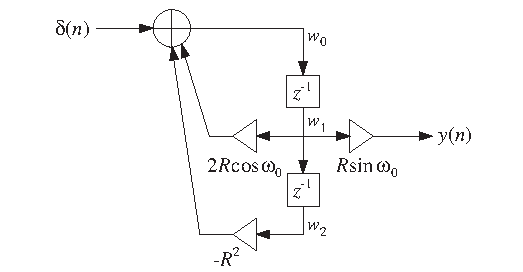
\includegraphics[width = 0.45\textwidth]{pic/sinusGen.pdf} & 
		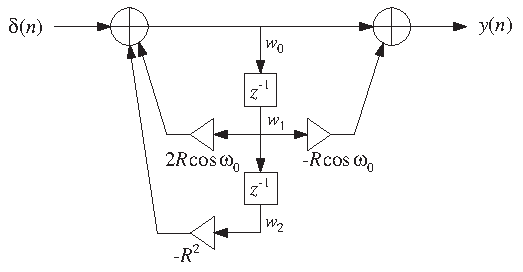
\includegraphics[width = 0.45\textwidth]{pic/cosinusGen.pdf}\\ 
		\fcolorbox{black}{white}{$\begin{array}{l}for\,\, n = 0,1,2,...\,\, do:\\
		\quad w_0 = 2R\cos(\omega_0)\,w_1 - R^2\,w_2 + \delta(n) \\
		\quad y = R\sin(\omega_0)\,w_1\\
		\quad w_2 = w_1\\
		\quad w_1 = w_0\end{array}$}& 
		\fcolorbox{black}{white}{$\begin{array}{l}for\,\, n = 0,1,2,...\,\, do:\\
		\quad w_0 = 2R\cos(\omega_0)\,w_1 - R^2\,w_2 + \delta(n) \\
		\quad y = w_0 - R\cos(\omega_0)\,w_1\\
		\quad w_2 = w_1\\
		\quad w_1 = w_0\end{array}$}\\[1.6cm]
	\hline\multicolumn{2}{|c|}{}\\[-0.3cm]
		\multicolumn{2}{|c|}{\textbf{Gekoppelter-Sinus-Cosinus-Generator}}\\[0.1cm]
	\hline\multicolumn{2}{|c|}{}\\[-0.2cm]
		\multicolumn{2}{|c|}{\fcolorbox{CadetRed}{white}{$h_1(n) = R^n\,\cos(\omega_0n)\,u(n)$}$\qquad$ \fcolorbox{CadetRed}{white}{$h_2(n) = R^n\,\sin(\omega_0n)\,u(n)$}}\\[0.35cm]
		\multicolumn{2}{|c|}{\fcolorbox{CadetRed}{white}{$H_1(z) = \dfrac{1 - a\,z^{-1}}{1-2\,a\,z^{-1}+(a^2+b^2)\,z^{-2}}$} $\qquad$ \fcolorbox{CadetRed}{white}{$H_2(z) = \dfrac{b\,z^{-1}}{1-2\,a\,z^{-1}+(a^2+b^2)\,z^{-2}}$}}\\[0.6cm]
		\multicolumn{2}{|c|}{\fcolorbox{CadetRed}{white}{$a = R\,\cos(\omega_0)$} $\qquad$ \fcolorbox{CadetRed}{white}{$b=R\,\sin(\omega_0)$}}\\[0.25cm]
		\multicolumn{2}{|c|}{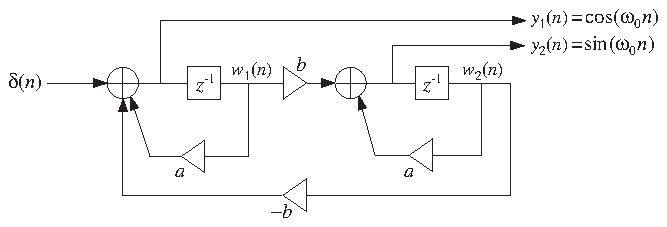
\includegraphics[width = 0.6\textwidth]{pic/sinusCosinusGen.pdf}}\\
		\multicolumn{2}{|c|}{\fcolorbox{black}{white}{$\begin{array}{l}for\,\, n = 0,1,2,...\,\, do:\\
		\quad y_1 = a\,w_1 - b\,w_2 + \delta(n) \\
		\quad y_2 = a\,w_2 + b\,w_1 \\
		\quad w_1 = y_1\\
		\quad w_2 = y_2\end{array}$}}\\[1.4cm]
	\hline
	\end{tabular}

\section{Periodische Waveform Generatoren}
	\subsection{Periodische Signale}
		\vspace*{-1.3cm}\begin{minipage}{0.6\textwidth}
			\begin{danger}
				Die abgetastete Version $x(n)$ eines periodischen Signals $x(t)$ ist nicht zwingend periodisch! 
			\end{danger}
		\end{minipage}\begin{minipage}{0.03\textwidth}$ $\end{minipage}
		\begin{minipage}{0.4\textwidth}
			\begin{tikzpicture}[>=latex', scale=3.3]
				\def\f{0.15};
				\draw[line width=0.5,->](-0.2,0)--++(2,0)node[right]{\small$t$};
				\draw[line width=0.5,->](0,-0.5)--++(0,1)node[right]{\small$x(t)$};
				\draw[smooth,samples=100,domain=0:1.7, CadetRed, line width=1] plot (\x,{0.35*sin(8*\x*180/pi)});
				\draw[smooth,samples=100,domain=-0.2:0, CadetRed, line width=1] plot (\x,{0});
				\foreach \i in {0,1,...,11}
				{
					\coordinate (sample) at ({\i*\f},{0.35*sin(8*\i*\f*180/pi)});
					\fill (sample) circle (0.65pt);
					\draw[line width=0.75](sample)--({\i*\f},0);
				}
				\draw[line width=0.5](0.787,0.05)--(0.787,-0.5);
				\draw[line width=0.5,<->](0,-0.43)--node[below]{\small$T_D$}++(0.787,0);

				\draw[line width=0.5](\f*3,0)--++(0,0.25);
				\draw[line width=0.5](\f*4,0)--++(0,0.25);
				\draw[line width=0.5,<->](\f*3,0.21)--node[above]{\small$T$}++(\f,0);

			\end{tikzpicture}
		\end{minipage}$ $\\[-1cm]
		Damit das abgetastete Signal $x(n)$ periodisch ist muss gelten:\\[0.15cm]
		\begin{tabular}{ll}
		 $\begin{array}{l}\text{$T_D$ ist ein ganzzahliges Vielfaches }\\\text{der Abtastperiode $T$}\end{array}$ & \fcolorbox{CadetRed}{white}{$T_D = D\cdot T$}$\quad\;\Rightarrow\quad\;$\fcolorbox{CadetRed}{white}{$f = \dfrac{f_s}{D}$}\\[0.5cm]
		 $\;\,$analoge Periodizität: & \fcolorbox{black}{white}{$x(t) = x(t + T_D)$}\\[0.2cm]
		 $\;\,$digitale Periodizität: & \fcolorbox{black}{white}{$x(nT) = x(nT + DT)  = x(nT + T_D)$}\\
		\end{tabular}\\
		
	\subsection{Realisierungsformen periodischer Waveform Generatoren}
		\begin{itemize}
		 \item Die ersten $D$-Samples ($h(0),...,h(D-1)$) mit einem FIR-Filter spezifizieren und das FIR-Filter periodisch mit Impulsen anregen ($\delta(n),\delta(n-D),\delta(n-2D),...$).
		 \item FIR-Filter $N(z)$:$\qquad\qquad\qquad\,$
		 \fcolorbox{CadetRed}{white}{$N(z) = b_0+b_1\,z^{-1}+b_2\,z^{-2}+...+b_{D-1}\,z^{-(D-1)}$}
		 \item Periodische Anregung $P(z)$:$\;\;\;\;\,$
		 \fcolorbox{CadetRed}{white}{$P(z) = 1 + z^{-D} + z^{-2D} + z^{-3D}+ ... = \dfrac{1}{1-z^{-D}}$}
		 \item Übertragungsfunktion $H(z)$:$\quad$
		 \fcolorbox{CadetRed}{white}{$H(z) = P(z)\cdot N(z) = \dfrac{b_0+b_1\,z^{-1}+b_2\,z^{-2}+...+b_{D-1}\,z^{-(D-1)}}{1-z^{-D}}$}
		 \item Impulsantwort $h(n)$:$\qquad\qquad\;\;\,$
		 \fcolorbox{CadetRed}{white}{$h(n) = \underbrace{h(n-D)}_{\text{weitere Perioden}} + \underbrace{b_0\,\delta(n)+b_1\,\delta(n-1)+...+b_{D-1}\,\delta(n-(D-1))}_{\text{1. Periode}}$}\\[0.2cm]
		 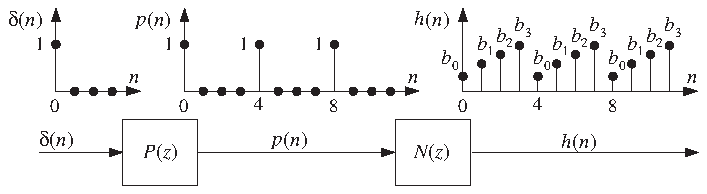
\includegraphics[width = 0.8\textwidth]{pic/periodischesDigitalesSignal.pdf}\\[-0.3cm]
		\end{itemize}
		
		\begin{minipage}{0.485\textwidth}
		\textbf{\textcolor{black}{\large{Implementierung mit Direktform}}}\\[-0.2cm]
			\begin{itemize}
			 \item Zustände $v_i$ und $w_i$ werden mit Null initialisiert.\\[-0.4cm]
			 \item FIR-Filter-Teil der angeregt wird, wodurch die ersten $D$ Samples generiert werden.\\[-0.4cm]
			 \item IIR-Filter-Teil der die $D$ Samples wiederholt.\\[-0.2cm]
			\end{itemize}
			\hspace*{0.3cm}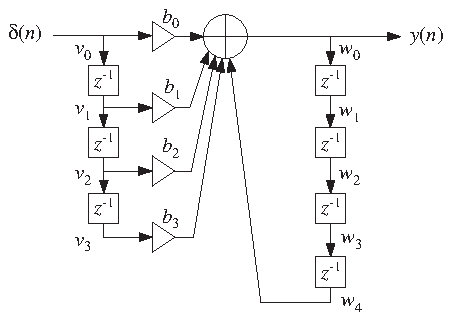
\includegraphics[width = 0.9\textwidth]{pic/periodischesWFGenDirektform.pdf}
		\end{minipage}\begin{minipage}{0.03\textwidth}$ $\end{minipage}
		\begin{minipage}{0.485\textwidth}
			\begin{tabular}{|lclll|}
			\hline &&&&$ $\\[-0.3cm]
			\multicolumn{5}{|l|}{$for\,\, n = 0,1,2,...\,\, do:$}\\
			&$v_0$&$ =$& $\delta(n)$&\\
			&$w_0$&$ = $&\multicolumn{2}{l|}{$b_0\,v_0 + b_1\,v_1 + b_2\,v_2 + ... + b_{D-1}\,v_{D-1}$}\\
			&$y$&$ =$&$ w_0$&\\
			&$v_i$&$ =$&$ v_{i-1}$ & $\qquad \quad i = D-1,\hdots,1$\\
			&$w_i$& $=$&$ w_{i-1}$ & $\qquad \quad i = D,D-1,\hdots,1$\\[0.1cm]
			\hline
			\end{tabular}\\[0.4cm]
			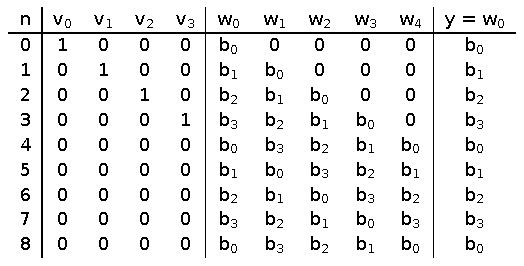
\includegraphics[width = \textwidth]{pic/TabelleDirektform.pdf}
		\end{minipage}

		\begin{minipage}{0.485\textwidth}
		\textbf{\textcolor{black}{\large{Implementierung mit kanonischer Form}}}\\[-0.2cm]
			\begin{itemize}
			 \item Zustände $w_i$ werden mit Null initialisiert.\\[-0.4cm]
			 \item FIR-Filter-Teil der periodisch angeregt wird, wodurch die $D$ Samples der Impulsantwort immer wieder generiert werden.\\[-0.4cm]
			 \item IIR-Filter-Teil der den Impuls $\delta(n)$ alle $D$ Samples wiederholt.\\[-0.1cm]
			\end{itemize}
			\hspace*{0.3cm}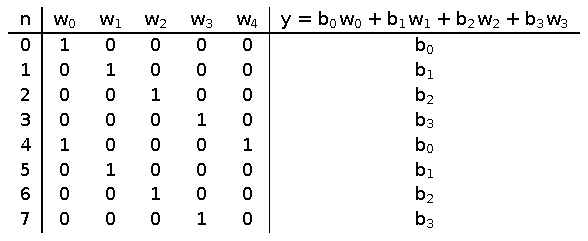
\includegraphics[width = \textwidth]{pic/TabelleKanonischeform.pdf}
		\end{minipage}\begin{minipage}{0.03\textwidth}$ $\end{minipage}
		\begin{minipage}{0.485\textwidth}
			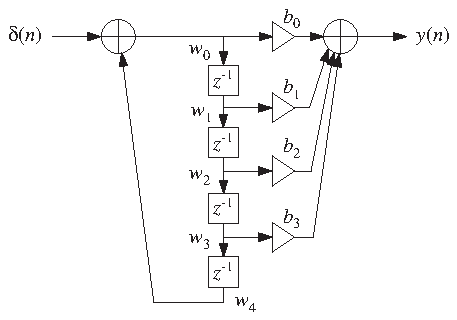
\includegraphics[width = 0.9\textwidth]{pic/periodischesWFGenKanonischeform.pdf}\\[0.1cm]
			\begin{tabular}{|lclll|}
			\hline &&&&$ $\\[-0.3cm]
			\multicolumn{5}{|l|}{$for\,\, n = 0,1,2,...\,\, do:$}\\
			&$w_0$&$ =$& $w_{D} + \delta(n)$&\\
			&$y$&$ = $&\multicolumn{2}{l|}{$b_0\,w_0 + b_1\,w_1 + b_2\,w_2 + ... + b_{D-1}\,w_{D-1}$}\\
			&$w_i$& $=$&$ w_{i-1}$ & $\qquad \quad i = D,D-1,\hdots,1$\\[0.1cm]
			\hline
			\end{tabular}
		\end{minipage}\\[0.1cm]
		
	\subsection{Spektrum periodischer Waveform Generatoren}
		\begin{itemize}
		 \item Da die Signalsequenzen $x(n)$ kausal (einseitig) sind, hat das Spektrum keine klaren Spektrallinien, sondern dominante Peaks bei der Grundfrequenz $f$ und dessen Harmonischen $mf$\\[0.2cm]
		 $H(\omega) = \dfrac{N(\omega)}{1-\e^{-j\omega D}} = \dfrac{N(\omega)}{2j\e^{j\omega D/2}\sin\left(\dfrac{\omega D}{2}\right)}\quad$\\[0.2cm]
		 $\Rightarrow\qquad$\fcolorbox{CadetRed}{white}{$\big|H(\omega)\big| = \dfrac{\big|N(\omega)\big|}{2\left|\sin\left(\dfrac{\omega D}{2}\right)\right|}$}$\quad$\fcolorbox{CadetRed}{white}{$\big|H(f)\big| = \dfrac{\big|N(f)\big|}{2\left|\sin\left(\dfrac{\pi fD}{f_s}\right)\right|}$}\\[-0.1cm]
		 \item Die Peaks kommen von den Polstellen von $|H(f)|$.\\[0.2cm]
		 $\sin\left(\dfrac{\pi fD}{f_s}\right) = 0\qquad\Rightarrow\quad\dfrac{\pi fD}{f_s}=m\pi$
		 $\qquad\Rightarrow\qquad$\fcolorbox{CadetRed}{white}{$f_m = m\dfrac{f_s}{D}\qquad\omega_m = \dfrac{2\pi m}{D}$}$\qquad m=0,1,...,D-1$
		 \\[0.3cm]
		 \begin{minipage}{0.75\textwidth}
			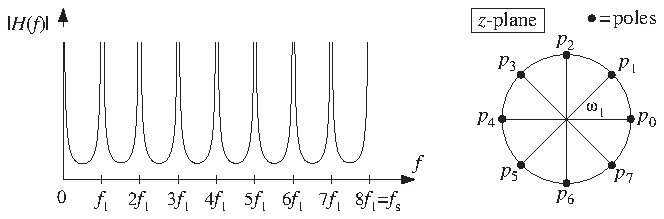
\includegraphics[width = \textwidth]{pic/SpektrumperiodischesDigitalesSignal.pdf}
		 \end{minipage}
		 \begin{minipage}{0.03\textwidth}$ $\end{minipage}
		 \begin{minipage}{0.27\textwidth}
			\fcolorbox{CadetRed}{white}{$z = p_m = \e^{j\omega_m}$}
		 \end{minipage}
		\end{itemize}
\newpage
\section{Wavetable Generatoren}
	\begin{itemize}
	 \item Statt zu filtern, können die $D$ Samples einer Periode auch in einer Tabelle abgespeichert werden und anschliessend immer wieder ''abgespielt'' werden.\\[-0.4cm]
	 \item Die Tabelle wird ein einem zirkularen Buffer $\bm{w} = [w_0,...,w_{D-1}]$ gespeichert und über einen Pointer $^*p = w[q]$, der rückwärts im Kreis wandert, ausgelesen.\\[-0.4cm]
	 \item Das Signal kann ganz einfach mit dem Startpunkt des Pointers $p$ verzögert werden:\\[0.1cm]
	 nicht verzögern:$\qquad$\fcolorbox{CadetRed}{white}{$p = \&w[0]$}$\qquad$um $m$-Samples verzögern:$\qquad$\fcolorbox{CadetRed}{white}{$p = \&w[m]$}\\[-0.4cm]
	 \item Der Buffer wird rückwärts gefüllt\\[0.15cm]
	 \fcolorbox{black}{white}{$\begin{array}{l}for\;i=0,1,...,D-1\;do:\\\quad w[(D-i)\%D] = b[i];\end{array}$}$\qquad$oder$\qquad$\fcolorbox{black}{white}{$\begin{array}{l}for\;i=0,1,...,D-1\;do:\\\quad w[i] = b[(D-i)\%D];\end{array}$}\\[-0.0cm]
	 \item Das Auslesen aus dem Buffer kann folgendermassen gemacht werden.\\[0.15cm]
	 \fcolorbox{black}{white}{$\begin{array}{l}q_0 = 0;\\ p = \& w[q_0];\\do\;\,forever:\\\quad y = *p;\\\quad q_{n+1} = (q_n-1)\%D;\\\quad p = \&w[q_{n+1}];\end{array}$}\\[-3.2cm]
	 \hspace*{4.6cm}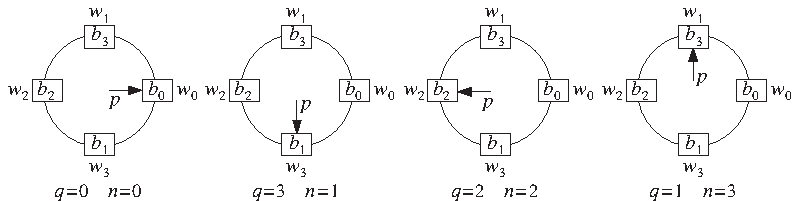
\includegraphics[width = 0.75\textwidth]{pic/wavetable4.pdf}\\[-0.2cm]
	\end{itemize}

	\subsection{Frequenz-Änderungen durch Wavetable-Manipulation}
		\begin{itemize}
		\item Die Abtastfrequenz $f_s$, die Länge der Wavetable $D$ und die Periode\\ $T_D$ bzw. die fundamentale Frequenz $f$ hängen folgendermassen\\ zusammen:\\[-1.1cm]
		\hspace*{12cm}\fcolorbox{CadetRed}{white}{$T_D = D\,T\qquad\Rightarrow\qquad f = \dfrac{f_s}{D}$}\\[-0.1cm]
		\item Die fundamentale Frequenz $f$ kann verändert werden,\\ indem die Länge der Wavetable $D$ verändert wird.\\[-1cm]
		\hspace*{10.6cm}\fcolorbox{CadetRed}{white}{$T_d = d\,T\qquad\Rightarrow\qquad f = \dfrac{f_s}{d}$}$\quad d\leq D$\\[-0.3cm]
		\item Wenn $D$ ein ganzzahliges Vielfaches von $d$ ist werden einfach Samples in der Wavetable übersprungen.\\
		\textbf{Beispiel:}\\ Nur jedes zweite Sample ausgeben$\quad\Rightarrow\quad$ fundamentale Frequenz $f$ verdoppeln.\\[-0.8cm]
		\hspace*{14.4cm}\fcolorbox{CadetRed}{white}{$c = \dfrac{D}{d}$}$\quad c\in\mathbb{Z}$\\[-0.1cm]
		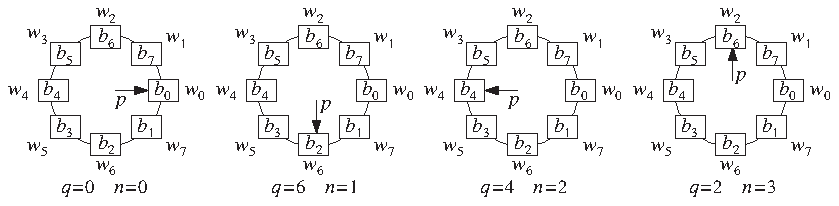
\includegraphics[width = 0.8\textwidth]{pic/wavetable6.pdf}\\[-0.6cm]
		\item Ist $D$ kein ganzzahliges Vielfaches von $d$ entstehen keine ganzzahligen Offsets und damit keine ganzzahligen Indizes $q_n$. Folglich müssen\\[-0.6cm]
		\begin{itemize}
		 \item Die Indizes aufgerundet, abgerundet oder normal gerundet werden.\\[-0.6cm]
		 \item Die Koeffizienten $b_i$ der Indizes davor und danach ($w\big[\lceil q_n\rceil\big],\,w\big[\lfloor q_n\rfloor\big]$) linear interpoliert werden. \\[-0.5cm]
		\end{itemize}
		\item Der Update des Indexes wird folgendermassen gemacht\\[0.1cm]
		\fcolorbox{CadetRed}{white}{$y(n)=\,\!^*p = w[q_n]$}$\qquad$\fcolorbox{CadetRed}{white}{$q_{n+1}=(q_n-c)\%D$}
		\end{itemize}
		\begin{danger}
		 \begin{tabularx}{\textwidth}{p{13cm}p{5cm}}
		  &\\[-0.8cm]
		  Damit das Abtasttheorem nicht verletzt wird muss $f$ innerhalb des Nyquist-Intervalls bleiben und für $c$ gilt damit: & $\begin{array}{l}\\[-0.1cm]\text{\fcolorbox{CadetRed}{white}{$-\dfrac{D}{2}\leq c \leq \dfrac{D}{2}$}}\end{array}$\\
		 \end{tabularx}
		\end{danger}	


\chapter{Rausch-Reduktion und Signal-Verbesserung \textcolor{black}{\small S.382}}
% 
% (c) Copyright 2016 Tabea Mendez
% 
% This source is free: you can redistribute it and/or modify
% it under the terms of the GNU General Public License as published by
% the Free Software Foundation, either version 3 of the License, or
% (at your option) any later version.
% 
% This source is distributed in the hope that it will be useful,
% but WITHOUT ANY WARRANTY; without even the implied warranty of
% MERCHANTABILITY or FITNESS FOR A PARTICULAR PURPOSE.  See the
% GNU General Public License for more details.
% 
% You should have received a copy of the GNU General Public License
% along with this source.  If not, see <http://www.gnu.org/licenses/>.
%
%%%%%%%%%%%%%%%%%%%%%%%%%%%%%%%%%%%%%%%%%%%%%%%%%%%%%%%%%%%%%%%%%%%%%%%%%%%%%%

\section{Rausch-Reduktions-Filter}
	\begin{goal}
	 \begin{minipage}{0.8\textwidth}
	 $ $\\Das Ziel eines Rausch-Reduktions-Filters $H(z)$ ist es, das eigentliche Signal $x_S(n)$ aus dem Messsignal $x(n)$ herauszufiltern und dabei das Rauschen $x_V(n)$ zu unterdrücken.\\
	 $\;\begin{array}{l}\text{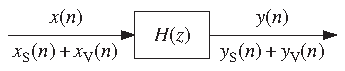
\includegraphics[width = 0.45\textwidth]{pic/NoiseRedFilterTime.pdf}}\end{array}\qquad$\fcolorbox{CadetRed}{white}{$\begin{array}{lcl}y_S(n) &= &x_S(n-delay)\\y_V(n) &=& 0\end{array}$}
	 \end{minipage}
	\end{goal}\\[-0.3cm]

	\subsection{Ideales Rausch-Reduktions-Filter}
		Damit das Rauschen vollkommen unterdrückt werden kann ohne das eigentliche Signal $x_S(n)$ zu verändern muss im Frequenzbereich folgendes gelten:\\
		\begin{minipage}{0.36\textwidth}
			\fcolorbox{CadetRed}{white}{$\begin{array}{l}Y_S(\omega)\; =\; H(\omega)\,X_S(\omega)\; =\; X_S(\omega)\\Y_V(\omega)\, = \;H(\omega)\,X_V(\omega) \,= \;0\end{array}$}\\[0.2cm]
			$\begin{array}{ll}\Rightarrow&\;\textbf{Die beiden Spektren $X_S(\omega)$}\\&\;\textbf{und $X_V(\omega)$ dürfen nicht}\\&\;\textbf{überlappen!}\end{array}$\\[0.2cm]
		\end{minipage}
		\begin{minipage}{0.67\textwidth}
		 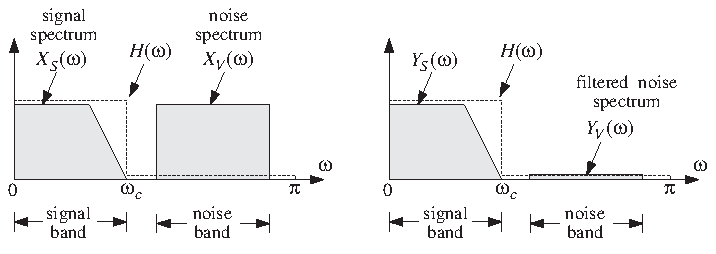
\includegraphics[width = \textwidth]{pic/NoiseRedFilterIdeal.pdf}
		\end{minipage}

	\subsection{Bestmögliches Rausch-Reduktions-Filter}
		Ist das ideale Rausch-Reduktions-Filter nicht realisierbar, weil die beiden Spektren $X_S(\omega)$ und $X_V(\omega)$ überlappen ist die bestmögliche Lösung ein \textbf{idealer Bandpass} (hier Tiefpass).\\[-0.5cm]
		\begin{itemize}
			 \item Das eigentliches Signal $x_S(n)$ wird nicht verzerrt.$\qquad$
			 \fcolorbox{CadetRed}{white}{$Y_S(\omega)\; =\; H(\omega)\,X_S(\omega)\; =\; X_S(\omega)$}\\[-0.5cm]
			 \item Das Rauschen $x_V(n)$ wird maximal unterdrückt.\\[-0.5cm]
			\end{itemize}
		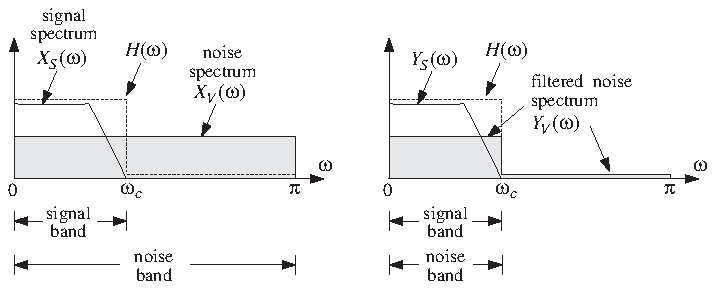
\includegraphics[width = 0.7\textwidth]{pic/NoiseRedFilter.pdf}\\[-0.1cm]
		\textbf{Rauschen:}\\[0.15cm]
		Für ein Mittelwertfreies-Weisses-Rauschen $x_V(n)$ gelten folgende Beziehungen:\\[0.2cm]
		\begin{tabular}{ll}
			Leistungsdichtespektrum und Leistung des&\multirow{2}{*}{\fcolorbox{CadetRed}{white}{$S_{X_VX_V}(\omega) = \sigma_{X_V}^2$}}\\
			Mittelwertfreiem-Weissem-Rauschen $x_V(n)$&\\[0.2cm]
			Leistungsdichtespektren des &\multirow{2}{*}{\fcolorbox{CadetRed}{white}{$S_{Y_VY_V}(\omega) =\big|H(\omega)\big|^2 \, S_{X_VX_V}(\omega)=\big|H(\omega)\big|^2 \, \sigma_{X_V}^2 $}}\\
			Farbigen-Ausgangsrauschen $y_V(n)$&\\[0.3cm]
			Leistung des Farbigen-Ausgangsrauschen&\fcolorbox{CadetRed}{white}{$\sigma_{Y_V}^2 = \dfrac{1}{2\pi}\myint{-\pi}{\pi}{S_{Y_VY_V}(\omega)}{\omega}= \sigma_{X_V}^2\dfrac{1}{2\pi}\myint{-\pi}{\pi}{\big|H(\omega)\big|^2}{\omega}= \sigma_{X_V}^2\,NRR$}\\[0.8cm]
			Noise-Reduction-Ratio NRR &\multirow{2}{*}{\fcolorbox{CadetRed}{white}{$NRR = \dfrac{\sigma_{Y_V}^2}{\sigma_{X_V}^2}= \dfrac{1}{2\pi}\myint{-\pi}{\pi}{\big|H(\omega)\big|^2}{\omega} = \mysum{n}{}{h(n)^2}$}}\\
			(sollte möglichst klein sein)&\\[0.3cm]
		\end{tabular}\\[0.2cm]
		\textbf{Signal-Rausch-Abstand SNR:}\\[0.2cm]
		Durch das Rausch-Reduktions-Filter ergeben sich folgende Signal-Rausch-Abstände:\\[0.2cm]
		\begin{tabular}{ll}
			SNR am Eingang & \fcolorbox{CadetRed}{white}{$\text{SNR}_{in} = \dfrac{E[x_S(n)^2]}{E[x_V(n)^2]} $}$\qquad\qquad\qquad$SNR am Ausgang $\quad$ \fcolorbox{CadetRed}{white}{$\text{SNR}_{out} = \dfrac{E[y_S(n)^2]}{E[y_V(n)^2]} $}\\[0.7cm]
			SNR-Verbesserung & \fcolorbox{CadetRed}{white}{$\dfrac{\text{SNR}_{out}}{\text{SNR}_{in}} = \dfrac{E[y_S(n)^2]}{E[y_V(n)^2]}\cdot \dfrac{E[x_V(n)^2]}{E[x_S(n)^2]}
			= \underbrace{\dfrac{E[x_V(n)^2]}{E[y_V(n)^2]}}_{1/NRR}\cdot \dfrac{E[y_S(n)^2]}{E[x_S(n)^2]}$}\\[1.3cm]
			&$\;\Rightarrow\quad$ Wenn das Signal $x_S(n)$ durch das Filter $H(\omega)$ nicht verändert wird gilt:\\[0.2cm]
			& $\qquad\quad$\fcolorbox{CadetRed}{white}{$\dfrac{\text{SNR}_{out}}{\text{SNR}_{in}} = \dfrac{1}{NRR}$}\\
		\end{tabular}\\[0.2cm]
		\textbf{NRR von idealen Filtern:}\\[0.2cm]
		\begin{tabular}{ll}
			Idealer Tiefpass & \fcolorbox{CadetRed}{white}{$NRR = \dfrac{\sigma_{Y_V}^2}{\sigma_{X_V}^2}= \dfrac{1}{2\pi}\myint{-\omega_c}{\omega_c}{1}{\omega} = \dfrac{2\omega_c}{2\pi} = \dfrac{\omega_c}{\pi}$}\\[0.8cm]
			Idealer Bandpass & \fcolorbox{CadetRed}{white}{$NRR = \dfrac{\sigma_{Y_V}^2}{\sigma_{X_V}^2}= \dfrac{2}{2\pi}\myint{\omega_a}{\omega_b}{1}{\omega} = \dfrac{\omega_b-\omega_a}{\pi}$}\\
		\end{tabular}\\[0.2cm]
	\subsection{Reale Rausch-Reduktions-Filter}
		Ideale Filter mit einer unendlich kurzen Übergangsbandbreite können nicht implementiert werden.\\
		Reale Rausch-Reduktions-Filter haben eine gewisse Übergangsbandbreite und sind oft linearphasig.\\[0.3cm]
		\begin{tabularx}{\textwidth}{|rp{4cm}p{9cm}X|}
		 \hline&&&\\[-0.3cm]
			\multicolumn{4}{|l|}{\textbf{IIR-Smoother erster Ordnung}}\\[-0.35cm]
			&&&
			\begin{tikzpicture}[>=latex, scale=1.2]
				\def\s{2.7};
				\def\f{1.15};
				\def\r{0.9};
				\def\roc{0.9};
				\coordinate (c1) at (0,0);
				\draw[line width=0.5](c1)++(-\s/2,-\s/2)node[above right]{ }--++(\s,0)--++(0,\s)node[below left]{\small$z$-Plane}--++(-\s,0)--cycle node[below right, CadetRed]{\textbf{ }};
				\draw[line width=0.75](c1)--++(-\f,0)--++(2*\f,0)--++(-\f,0)--++(0,-\f)--++(0,2*\f)--++(0,-\f)circle(0);
				\draw[line width=0.75,dashed](c1)circle(\roc);
				\draw[line width=0.75](c1)++(\roc,0.1)--++(0,-0.2)node[below right=-3pt,yshift=2pt]{$1$};
				\draw[line width=0.75](c1)++(-\roc,0.1)--++(0,-0.2)node[below left=-3pt,yshift=2pt]{\small-$1$};
				\draw[line width=0.75,fill,CadetRed](c1)++(0.65,0)circle(\r/15)node[below=2pt]{\small$a$};
% 				\draw[CadetRed,line width=0.75,fill=white](c1)++(0.75,-0.5)circle(\r/15)node[below left=-2pt]{$z_1$};

			\end{tikzpicture}\\[-2.85cm]
			$\;\,\bullet\!\!\!$ & \multicolumn{2}{p{13cm}}{Geeignet für DC-Signale $x_S(n)$}&\\[0.25cm]
			$\;\,\bullet\!\!\!$ & \multicolumn{2}{p{13cm}}{Mittelung über alle bisherigen Samples, wobei die Samples mit dem Faktor $a^d\,b\,x(n-d)$ gewichtet werden. Je weiter ein Sample zurückliegt, desto weniger } &\\
			&Einfluss hat es.&\fcolorbox{CadetRed}{white}{$y(n) = b\,x(n) + a\,y(n-1)$}$\qquad$\fcolorbox{black}{white}{$b = 1-a$}&\\[0.3cm]
			$\;\,\bullet\!\!\!$ &  Signalband:&\fcolorbox{black}{white}{$\omega = 0$}&\\[0.2cm]
			$\;\,\bullet\!\!\!$ & Übertragungsfunktion: &\fcolorbox{CadetRed}{white}{$H(z) = \dfrac{b}{1-a\,z^{-1}}\qquad\Rightarrow\qquad \big|H(\omega)\big|^2 =\dfrac{b^2}{1-2\,a\cos(\omega) + a^2}$}&\\[0.6cm]
			$\;\,\bullet\!\!\!$ & Grenzfrequenz: &\fcolorbox{CadetRed}{white}{$\big|H(\omega_c)\big|^2 = \dfrac{1}{2}\qquad\Rightarrow\qquad \cos(\omega_c) = 1-\dfrac{(1-a)^2}{2\,a}$}&\\[0.5cm]
			$\;\,\bullet\!\!\!$ & DC- und AC-Gain: &\fcolorbox{CadetRed}{white}{DC:$\;\;H(z)\big|_{z=1} = \dfrac{b}{1-a} = 1\qquad$AC:$\;\; H(z)\big|_{z=-1} = \dfrac{1-a}{1+a}$}&\\[0.5cm]
			$\;\,\bullet\!\!\!$ & Noise-Reduction-Ratio: &\fcolorbox{CadetRed}{white}{$NRR = \dfrac{1-a}{1+a}$}$\begin{array}{l}\text{$\qquad\quad\!$ Einschwingzeit:$\qquad$\fcolorbox{CadetRed}{white}{ $n_\text{eff} = \dfrac{\ln(\epsilon)}{\ln(a)}$}}\end{array}$&\\[0.6cm]
		\hline
		\end{tabularx}
		\begin{tabularx}{\textwidth}{|rp{4cm}p{9cm}X|}
		\hline&&&\\[-0.3cm]
			\multicolumn{4}{|l|}{\textbf{IIR-Smoother erster Ordnung mit bestimmter Grenzfrequenz}}\\[-0.35cm]
			&&&
			\begin{tikzpicture}[>=latex, scale=1.2]
				\def\s{2.7};
				\def\f{1.15};
				\def\r{0.9};
				\def\roc{0.9};
				\coordinate (c1) at (0,0);
				\draw[line width=0.5](c1)++(-\s/2,-\s/2)node[above right]{ }--++(\s,0)--++(0,\s)node[below left]{\small$z$-Plane}--++(-\s,0)--cycle node[below right, CadetRed]{\textbf{ }};
				\draw[line width=0.75](c1)--++(-\f,0)--++(2*\f,0)--++(-\f,0)--++(0,-\f)--++(0,2*\f)--++(0,-\f)circle(0);
				\draw[line width=0.75,dashed](c1)circle(\roc);
				\draw[line width=0.75](c1)++(\roc,0.1)--++(0,-0.2)node[below right=-3pt,yshift=2pt]{$1$};
				\draw[line width=0.75](c1)++(-\roc,0.1)--++(0,-0.2)node[below left=-3pt,yshift=2pt]{\small-$1$};
				\draw[line width=0.75,fill,CadetRed](c1)++(0.65,0)circle(\r/15)node[below=2pt]{\small$a$};
				\draw[CadetRed,line width=0.75,fill=white](c1)++(-0.9,0)circle(\r/15);%node[below left=-2pt]{$z_1$};

			\end{tikzpicture}\\[-2.85cm]
			$\;\,\bullet\!\!\!$ & \multicolumn{2}{p{13cm}}{Geeignet für DC-Signale $x_S(n)$}&\\[0.25cm]
			$\;\,\bullet\!\!\!$ & \multicolumn{2}{p{13cm}}{Mittelung über alle bisherigen Samples, wobei die Samples mit dem Faktor $(a^d+a^{d-1})\,b\,x(n-d)$ gewichtet werden. Je weiter ein Sample zurückliegt, desto} &\\
			&weniger Einfluss hat es.&\fcolorbox{CadetRed}{white}{$y(n) = b\,x(n) +b\,x(n-1) + a\,y(n-1)$}&\\[0.2cm]
			&&\fcolorbox{black}{white}{$a = \dfrac{1-\tan(\omega_c/2)}{1+\tan(\omega_c/2)}$}$\qquad$\fcolorbox{black}{white}{$b = \dfrac{1-a}{2}$}&\\[0.6cm]
			$\;\,\bullet\!\!\!$ &  Signalband:&\fcolorbox{black}{white}{$\omega = 0$}&\\[0.25cm]
			$\;\,\bullet\!\!\!$ & Übertragungsfunktion: &\fcolorbox{CadetRed}{white}{$H(z) = \dfrac{b\,(1+z^{-1})}{1-a\,z^{-1}}\qquad\Rightarrow\qquad \big|H(\omega)\big|^2 =\dfrac{2b^2(1+\cos(\omega))}{1-2\,a\cos(\omega) + a^2}$}&\\[0.6cm]
			$\;\,\bullet\!\!\!$ & Grenzfrequenz: &\fcolorbox{CadetRed}{white}{$\big|H(\omega_c)\big|^2 = \dfrac{1}{2}\qquad\Rightarrow\qquad \cos(\omega_c) = \dfrac{2\,a}{1+a^2}$}&\\[0.5cm]
			$\;\,\bullet\!\!\!$ & DC- und AC-Gain: &\fcolorbox{CadetRed}{white}{DC:$\;\;H(z)\big|_{z=1} = \dfrac{2b}{1-a} = 1\qquad$AC:$\;\; H(z)\big|_{z=-1} = 0$}&\\[0.5cm]
			$\;\,\bullet\!\!\!$ & Noise-Reduction-Ratio: &\fcolorbox{CadetRed}{white}{$NRR = \dfrac{1-a}{2}$}$\begin{array}{l}\text{$\qquad\quad\!$ Einschwingzeit:$\qquad$\fcolorbox{CadetRed}{white}{ $n_\text{eff} = \dfrac{\ln(\epsilon)}{\ln(a)}$}}\end{array}$&\\[0.6cm]
		 \hline&&&\\[-0.3cm]
			\multicolumn{4}{|l|}{\textbf{FIR-Mittelungs-Filter}}\\[-0.35cm]
			&&&
			\hspace*{-0.2cm}\begin{tikzpicture}[>=latex, scale=1.2]
				\def\s{2.7};
				\def\f{1.15};
				\def\r{0.9};
				\def\roc{0.9};
				\def\n{11};
				\coordinate (c1) at (0,0);
				\draw[line width=0.5](c1)++(-\s/2,-\s/2)node[above right,yshift=-3pt]{\footnotesize $k=1,2,...,N-1$}--++(\s,0)--++(0,\s)node[below left]{\small$z$-Plane}--++(-\s,0)--cycle node[below right, CadetRed]{\textbf{ }};
				\draw[line width=0.75](c1)--++(-\f,0)--++(2*\f,0)--++(-\f,0)--++(0,-\f)--++(0,2*\f)--++(0,-\f)circle(0);
				\draw[line width=0.75,dashed](c1)circle(\roc);
				\draw[line width=0.75](c1)++(\roc,0.1)--++(0,-0.2)node[below right=-3pt,yshift=2pt]{$1$};
				\draw[line width=0.75](c1)++(-\roc,0.1)--++(0,-0.2)node[below left=-3pt,yshift=2pt]{-$1$};

				\draw[line width=2,white](c1)++(\s/2,0)--++(0,0.65);

				\draw[line width=0.75,dotted](c1)--++({360*0/\n}:1.2);
				\draw[line width=0.75,->](c1)++({360*0/\n}:1.05)arc({360*0/\n}:{360*1/\n}:1.05)node[below right, xshift=3pt,yshift=5pt]{\Large$\frac{2\pi k}{N}$};
				\draw[line width=0.75,dotted](c1)--++({360*1/\n}:1.2);



% 				\draw[line width=0.75,fill,CadetRed](c1)++(0.65,0)circle(\r/15)node[below=2pt]{\small$a$};
				\foreach \i in {1,2,...,10}
				{
					\draw[CadetRed,line width=0.75,fill=white](c1)++({360*\i/\n}:0.9)circle(\r/15);
				}
			\end{tikzpicture}\\[-2.85cm]
			$\;\,\bullet\!\!\!$ & \multicolumn{2}{p{13cm}}{Geeignet für DC-Signale und tieffrequente Signale $x_S(n)$}&\\[0.25cm]
			$\;\,\bullet\!\!\!$ & \multicolumn{2}{p{13cm}}{Mittelung über die letzten $N$ Samples, wobei alle gleich stark gewichtet werden ($1/N$), da dadurch die $NNR$ minimiert wird.} &\\[0.6cm]
			&\multicolumn{2}{p{13cm}}{\fcolorbox{CadetRed}{white}{$y(n) = \dfrac{1}{N}\big(x(n)+x(n-1)+x(n-2)+...+x(n-(N-1))\big)$}}&\\[0.5cm]
			$\;\,\bullet\!\!\!$ &  Signalband:&\fcolorbox{black}{white}{$0\leq\omega\leq\omega_c$}&\\[0.25cm]
			$\;\,\bullet\!\!\!$ & Übertragungsfunktion: &\fcolorbox{CadetRed}{white}{$H(z) = \dfrac{1}{N}\big(1+z^{-1}+...+z^{-(N-1)}\big)=\dfrac{1}{N}\,\dfrac{1-z^{-N}}{1-z^{-1}}$}&\\[0.6cm]
			$\;\,\bullet\!\!\!$ & Frequenzgang: &\fcolorbox{CadetRed}{white}{$\big|H(\omega)\big|^2 =\dfrac{1}{N^2}\,\dfrac{\sin^2(N\omega/2)}{\sin^2(\omega/2)}$}&\\[0.6cm]
			$\;\,\bullet\!\!\!$ & Grenzfrequenz: &\fcolorbox{CadetRed}{white}{$\big|H(\omega_c)\big|^2 \;\stackrel{\mathrm{N \text{ gross}}}\approx\; \dfrac{4}{\pi^2}\approx 0.41\;\;\widehat=\;\; 3.9\db\qquad\Rightarrow\qquad \omega_c = \dfrac{\pi}{N}$}&\\[0.5cm]
			$\;\,\bullet\!\!\!$ & DC- und AC-Gain: &\fcolorbox{CadetRed}{white}{DC:$\;\;H(z)\big|_{z=1}  = 1\qquad$AC:$\;\; H(z)\big|_{z=-1} =\small\begin{cases} 0,& N\text{ gerade}\\ 1/N,& N\text{ ungerade}\end{cases}$}&\\[0.6cm]
			$\;\,\bullet\!\!\!$ & Noise-Reduction-Ratio: &\fcolorbox{CadetRed}{white}{$NRR = \dfrac{1}{N}$}$\begin{array}{l}\text{$\qquad\quad\!$ Einschwingzeit:$\qquad$\fcolorbox{CadetRed}{white}{ $n_\text{eff} = N$}}\end{array}$&\\[0.5cm]
		 \hline
		\end{tabularx}
\newpage
			
\section{Notch- und Comb-Filter}
	Diese Filter sind gut geeignet, wenn das Rauchen $x_V(n)$ oder das Signal $x_S(N)$ periodisch sind.\\[-0.6cm]
	\begin{itemize}
	 \item \textbf{Notch-Filter:} Das periodische Rauschen (50 Hz Netzbrummen) wird durch Notches (Kerben) bei den Rauschfrequenzen vernichtet.\\[-0.6cm]
	 \item \textbf{Comb-Filter:} Die Spektrallinien des periodische Signal werden durch die Combs herausgefiltert und das umliegende Rauschen wird vernichtet.\\[-0.6cm]	 
	 \item Die Abtastfrequenz $f_s$ wird am besten auf ein ganzzahliges Vielfaches der\\ fundamentalen Frequenz $f$ (Signal- oder Rauschfrequenz) gesetzt.\\[-0.75cm] \hspace*{13cm}\fcolorbox{CadetRed}{white}{$f_s = D\cdot f$}\\[-0.35cm]
	 \item Ein Multi-Notch/Comb-Filter kann aus einem einfachen\\Filter erster Ordnung abgeleitet werden, indem $z$ durch \\$z^{D}$ ersetzt wird. Dadurch wird das periodische Spektrum\\ um den Faktor $D$ zusammen gestaucht.\\[-1.8cm]
	  \hspace*{11cm}\fcolorbox{CadetRed}{white}{$z\;\rightarrow\; z^{D}\quad\Rightarrow\quad H(\omega)\;\rightarrow\;H(\omega D)$}\\[0.1cm]
	  \hspace*{10cm}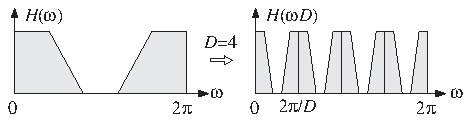
\includegraphics[width = 0.45\textwidth]{pic/combNotchStauchung.pdf}\\[-1.4cm]
	\end{itemize}
	\subsection{Notch-Filter}
		\vspace*{-0.3cm}\begin{minipage}{0.625\textwidth}
			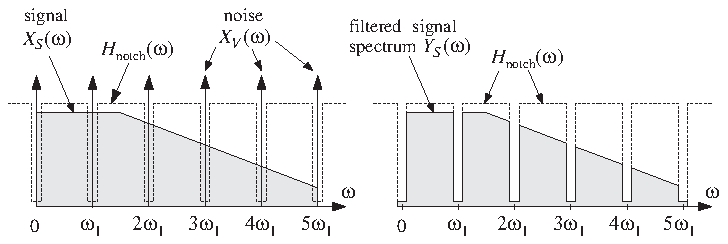
\includegraphics[width = \textwidth]{pic/notchFilter.pdf}\\[1.9cm]
		\end{minipage}\begin{minipage}[t]{0.075\textwidth}$ $\end{minipage}
		\begin{minipage}{0.3\textwidth}
			$\qquad$\begin{tikzpicture}[>=latex, scale=1.6]
				\def\s{2.7};
				\def\f{1.15};
				\def\r{0.9};
				\def\roc{0.9};
				\def\n{11};
				\coordinate (c1) at (0,0);
				\draw[line width=0.5](c1)++(-\s/2,-\s/2)--node[above,yshift=-1pt,xshift=-8pt]{\footnotesize$k=0,1,2,...,D-1$}++(\s,0)--++(0,\s)node[below left]{\small$z$-Plane}--++(-\s,0)--cycle node[below right, CadetRed]{\textbf{ }};
				\draw[line width=0.75](c1)--++(-\f,0)--++(2*\f,0)--++(-\f,0)--++(0,-\f)--++(0,2*\f)--++(0,-\f)circle(0);
				\draw[line width=0.5,dashed](c1)circle(\roc);
				\draw[line width=0.5,dashed](c1)circle(0.7);
				\draw[line width=0.75](c1)++(\roc,0.1)--++(0,-0.2)node[below right=-1pt,yshift=2pt]{$1$};
				\draw[line width=0.75](c1)++(-\roc,0.1)--++(0,-0.2)node[below left=-1pt,yshift=2pt]{-$1$};
				\draw[line width=0.75](c1)++(0.7,0.1)--++(0,-0.2);


				\draw[line width=2,white](c1)++(\s/2,0)++(0,0.05)--++(0,0.5);

				\draw[line width=0.75,dotted](c1)--++({360*0/\n}:1.2);
				\draw[line width=0.75,->](c1)++({360*0/\n}:1.1)arc({360*0/\n}:{360*1/\n}:1.1)node[below right, xshift=5pt,yshift=0pt]{\Large$\frac{2\pi k}{D}$};
				\draw[line width=0.75,dotted](c1)--++({360*1/\n}:1.2);



				
				\foreach \i in {0,1,2,...,10}
				{
					\draw[line width=0.75,dotted](c1)--++({360*\i/\n}:1);
					\draw[CadetRed,line width=0.75,fill=white](c1)++({360*\i/\n}:0.9)circle(\r/15);
					\draw[line width=0.75,fill,CadetRed](c1)++({360*\i/\n}:0.7)circle(\r/15);
				}

				\draw[line width=1,white](c1)++({360*10/\n}:0.3)--++({360*10/\n}:0.3);

				\draw[line width=0.75](c1)++(0.7,0.1)node[black,below left,yshift=-2pt]{$\sqrt[n]{a}$};

			\end{tikzpicture}
		\end{minipage}\\[-2.15cm]
		\begin{tabular}{ll}
			$3\,\db$-Bandbreite $\Delta\omega$: & \fcolorbox{CadetRed}{white}{$\beta = \tan\left(\dfrac{D\Delta\omega}{4}\right),\qquad a=\dfrac{1-\beta}{1+\beta},\qquad b = \dfrac{1}{1+\beta}$}\\[0.5cm]
			&$\begin{array}{l}0\leq a<1\\0<\beta\leq 1\end{array}\quad\Rightarrow\quad\Delta\omega \leq\dfrac{\pi}{D}\quad\Rightarrow\quad \Delta f\leq\dfrac{f_s}{2D}$\\[0.4cm]
			Übertragungsfunktion: &\fcolorbox{CadetRed}{white}{$H_{\text{notch}}(z) = b\dfrac{1-z^{-D}}{1-a\,z^{-D}}$}$\quad\;$\fcolorbox{CadetRed}{white}{$\big| H_{\text{notch}}(\omega)\big|^2 = \dfrac{\tan^2(\omega D/2)}{\tan^2(\omega D/2)+\beta^2}$}$\quad\;$ \fcolorbox{CadetRed}{white}{$NRR =b=\dfrac{1+a}{2}$}
		\end{tabular}

	\subsection{Comb-Filter}
		\vspace*{-0.3cm}\begin{minipage}{0.625\textwidth}
			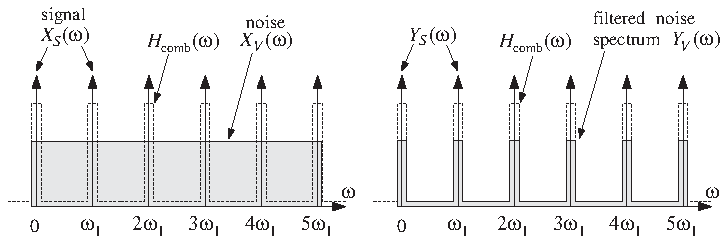
\includegraphics[width = \textwidth]{pic/combFilter.pdf}\\[1.9cm]
		\end{minipage}\begin{minipage}[t]{0.075\textwidth}$ $\end{minipage}
		\begin{minipage}{0.3\textwidth}
			$\qquad$\begin{tikzpicture}[>=latex, scale=1.6]
				\def\s{2.7};
				\def\f{1.15};
				\def\r{0.9};
				\def\roc{0.9};
				\def\n{11};
				\coordinate (c1) at (0,0);
				\draw[line width=0.5](c1)++(-\s/2,-\s/2)--node[above,yshift=-1pt,xshift=-8pt]{\footnotesize$k=0,1,2,...,D-1$}++(\s,0)--++(0,\s)node[below left]{\small$z$-Plane}--++(-\s,0)--cycle node[below right, CadetRed]{\textbf{ }};
				\draw[line width=0.75](c1)--++(-\f,0)--++(2*\f,0)--++(-\f,0)--++(0,-\f)--++(0,2*\f)--++(0,-\f)circle(0);
				\draw[line width=0.5,dashed](c1)circle(\roc);
				\draw[line width=0.5,dashed](c1)circle(0.7);
				\draw[line width=0.75](c1)++(\roc,0.1)--++(0,-0.2)node[below right=-1pt,yshift=2pt]{$1$};
				\draw[line width=0.75](c1)++(-\roc,0.1)--++(0,-0.2)node[below left=-1pt,yshift=2pt]{-$1$};
				\draw[line width=0.75](c1)++(0.7,0.1)--++(0,-0.2);


				\draw[line width=2,white](c1)++(\s/2,0)++(0,0.075)--++(0,0.45);
				\draw[line width=0.75,->](c1)++({360*0/\n}:1.15)node[above right, xshift=-3pt,yshift=1.5pt]{\Large$\frac{2\pi k}{D}$}arc({360*0/\n}:{360*1/\n}:1.1);
				\draw[line width=0.75,dotted](c1)--++({360*1/\n}:1.25);

				\draw[line width=2,white](c1)++(\s/2,0)++(0,-0.4)--++(0,-0.475);
				\draw[line width=0.75,->](c1)++({360*0/\n}:1.15)--++(0:0.05)--++(0:-0.05)node[below right, xshift=-10pt,yshift=-15pt]{\Large-$\frac{2\pi k+\pi}{D}$}arc({360*0/\n}:{-360*2/\n+180/\n}:1.1);
				\draw[line width=0.75,dotted](c1)--++({-360*2/\n+180/\n}:1.25);


				
				\foreach \i in {0,1,2,...,10}
				{
					\draw[line width=0.75,dotted](c1)--++({360*\i/\n}:1);
					\draw[CadetRed,line width=0.75,fill=white](c1)++({360*\i/\n+180/\n}:0.9)circle(\r/15);
					\draw[line width=0.75,fill,CadetRed](c1)++({360*\i/\n}:0.7)circle(\r/15);
				}

				\draw[line width=1,white](c1)++({360*10/\n}:0.3)--++({360*10/\n}:0.3);

				\draw[line width=0.75](c1)++(0.7,0.1)node[black,below left,yshift=-2pt]{$\sqrt[n]{a}$};

			\end{tikzpicture}
		\end{minipage}\\[-2.15cm]
		\begin{tabular}{ll}
			$3\,\db$-Bandbreite $\Delta\omega$: & \fcolorbox{CadetRed}{white}{$\beta = \tan\left(\dfrac{D\Delta\omega}{4}\right),\qquad a=\dfrac{1-\beta}{1+\beta},\qquad b = \dfrac{\beta}{1+\beta}$}\\[0.5cm]
			&$\begin{array}{l}0\leq a<1\\0<\beta\leq 1\end{array}\quad\Rightarrow\quad\Delta\omega \leq\dfrac{\pi}{D}\quad\Rightarrow\quad \Delta f\leq\dfrac{f_s}{2D}$\\[0.4cm]
			Übertragungsfunktion: &\fcolorbox{CadetRed}{white}{$H_{\text{comb}}(z) = b\dfrac{1+z^{-D}}{1-a\,z^{-D}}$}$\quad\;$\fcolorbox{CadetRed}{white}{$\big| H_{\text{comb}}(\omega)\big|^2 = \dfrac{\beta^2}{\tan^2(\omega D/2)+\beta^2}$}$\quad\;$ \fcolorbox{CadetRed}{white}{$NRR = b=\dfrac{1-a}{2}$}
		\end{tabular}
		
		\begin{info}
		 Die Noise-Reduction-Ratio bleibt gleich, wenn das Spektrum nur gestaucht wird. D.h. Die NNR der Notch- und Comb-Filter entspricht der NNR der entsprechenden Filter erster Ordnung.
		\end{info}

\newpage
\section{Signal-Mittelung }
	\begin{goal}
	 Von einem periodischen verrauschten Signal werden die Perioden gemittelt um das Rauschen zu unterdrücken. Diese Methode der Rauschunterdrückung resultiert in einem FIR-Comb-Filter und wird für die Verarbeitung von endlich langen Signal-Aufzeichnungen verwendet. 
	\end{goal}\\[-0.6cm]
	
	\begin{minipage}{0.6\textwidth}
		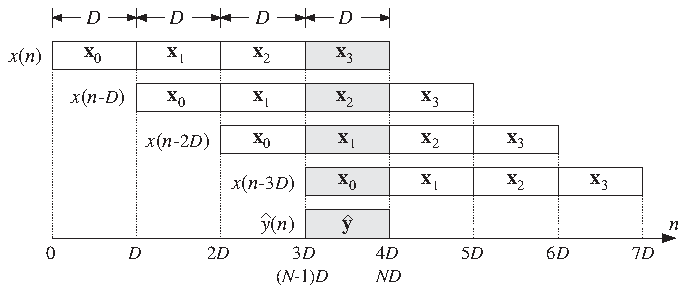
\includegraphics[width = \textwidth]{pic/signalAveraging1.pdf}
	\end{minipage}
	\begin{minipage}{0.4\textwidth}
		$\Rightarrow\quad$ \fcolorbox{CadetRed}{white}{$\begin{array}{l}\textbf{Mittelung über $\bm{N}$ Perioden}\\\textbf{mit der Länge $D$}\end{array}$}\\[0.4cm]
	\end{minipage}\\[0.2cm]
	\begin{tabular}{ll}
	 Gemitteltes Signal: & \fcolorbox{CadetRed}{white}{$\widehat{y}(n) = \dfrac{1}{N}\mysum{i=0}{N-1}{x(n-i\,D)}=\dfrac{1}{N}\mysum{i=0}{N-1}{x_i(n)} $}$\qquad n=0,1,2,...,D-1$\\[0.5cm]
	 Übertragungsfunktion: $\quad$& \fcolorbox{CadetRed}{white}{$H(z) = \dfrac{1}{N}(1+z^{-D}+z^{-2D}+...+z^{-(N-1)D}) = \dfrac{1}{N}\,\dfrac{1-z^{-ND}}{1-z^{-D}}$}\\[0.5cm]
	 Frequenzgang: & \fcolorbox{CadetRed}{white}{$H(\omega) = \dfrac{1}{N}\dfrac{\sin(ND\omega/2)}{\sin(D\omega/2)}$}$\qquad\quad$\fcolorbox{CadetRed}{white}{$\big|H(\omega)\big|^2 = \dfrac{1}{N^2}\dfrac{\sin^2(ND\omega/2)}{\sin^2(D\omega/2)}$}\\[0.5cm]
	 Grenzfrequenz: & \fcolorbox{CadetRed}{white}{$\omega_c = \dfrac{\pi}{ND}$}\\[0.5cm]
	 Noise-Reduction-Ratio:&\fcolorbox{CadetRed}{white}{$NRR = \dfrac{1}{N}$}
	\end{tabular}\\[0.2cm]
	
	\begin{info}
	 Dieses Filter erhält man auch, wenn man das Spektrum des FIR-Mittelungs-Filter $y(n) = [x(n)+x(n-1)+...+x(n-(N-1))]/N$ um den Faktor $D$ staucht ($z$ durch $z^D$ ersetzen)
	\end{info}
	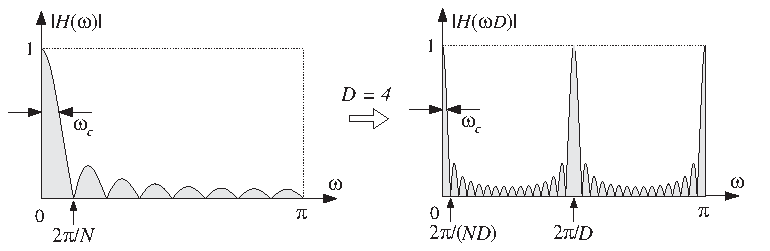
\includegraphics[width = 0.7\textwidth]{pic/signalAveraging.pdf}

	 Es resultiert ein Ausgangssignal das um den Faktor $1/N$ weniger stark rauscht.\\[0.2cm]
	 \fcolorbox{CadetRed}{white}{$\begin{array}{lcl}\widehat{y}(n)& =& y_S(n)+y_V(n)\\& = &x_S(n)+y_V(n)\end{array}$}$\qquad$
	 \fcolorbox{CadetRed}{white}{$\sigma_{Y_V}^2 = \dfrac{1}{N}\sigma_{X_V}^2$}\\

\newpage
\section{Savitzky-Golay-Smoothing-Filter}
	\begin{goal}
	 Die Idee ist, ein Polynom $p$-ter Ordnung optimal (Least-Square) in $N = 2M+1$ gemessene Samples einzupassen und anschliessend das mittlere Sample durch den Wert des Polynoms an dieser Stelle zu ersetzen. Dadurch wird das Rauschen reduziert. Zudem muss gelten $\quad$\fcolorbox{CadetRed}{white}{$N\geq p+1$}
	\end{goal}

	\textbf{Polynom-Beispiele mit N=5 Samples:}\\[0.2cm]
	\begin{tabularx}{\textwidth}{>{\centering\arraybackslash}X|>{\centering\arraybackslash}X|>{\centering\arraybackslash}X>{\centering\arraybackslash}X}
	 Konstante: & Linear: & Quadratisch: & \\[0.1cm]
	 \fcolorbox{CadetRed}{white}{$ \widehat{x}_m = c_0 $}&\fcolorbox{CadetRed}{white}{$\widehat{x}_m = c_0 + c_1\,m$}&\fcolorbox{CadetRed}{white}{$\widehat{x}_m = c_0 + c_1\,m+c_2\,m^2$}&\\
	 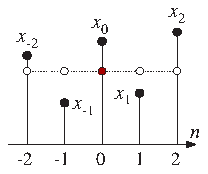
\includegraphics[width = 0.23\textwidth]{pic/SavitzkyGolayKonst.pdf} & 
	 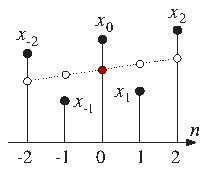
\includegraphics[width = 0.23\textwidth]{pic/SavitzkyGolayLin.pdf} & 
	 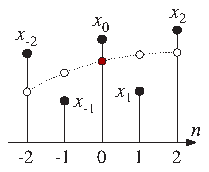
\includegraphics[width = 0.23\textwidth]{pic/SavitzkyGolayQuad.pdf} &
	 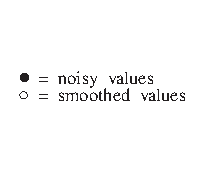
\includegraphics[width = 0.23\textwidth]{pic/SavitzkyGolayLeg.pdf}\\
	\end{tabularx}

	\subsection{Optimierungsproblem}
		Das Ziel ist ein Polynom $p$-ten Grades zu finden, welches den kleinsten quadratischen Fehler hat.\\[0.2cm]
		Minimiere:$\qquad$\fcolorbox{CadetRed}{white}{$\mathcal{J}\; = \mysum{m=-M}{M}{e_m^2}\;\; = \mysum{m=-M}{M}{(x_m - \widehat{x}_m)^2} = \mysum{m=-M}{M}{(x_m-(c_0 + c_1\,m + c_2\,m^2 + ... + c_p\,m^p))^2}$}\\[0.2cm]
		oder in Matrixschreibweise: $\qquad$\fcolorbox{CadetRed}{white}{$\mathcal{J} \;=\; \vec{e}\,^{\mathsf T}\vec e \;=\;(\vec x-S\,\vec c\,)^{\mathsf T}(\vec x-S\,\vec c\,) \;=\; \vec x\,^{\mathsf T}\vec x \;-\;2\,\vec c\,^{\mathsf T}S\,^{\mathsf T}\vec x\; +\; \vec c\,^{\mathsf T}S\,^{\mathsf T}S\,\vec c$}\\[0.2cm]
		\hspace*{2.6cm}mit $\qquad$ \fcolorbox{black}{white}{
		$\quad\vec c =\begin{bmatrix}c_0\\c_1\\c_2\\\vdots\\ c_p \end{bmatrix}$,
		$\qquad\vec x =\begin{bmatrix}x_{-M}\\\vdots\\x_{-1}\\x_0\\x_1\\\vdots\\ x_M \end{bmatrix}$,
		$\qquad\vec{ \widehat{x} }=\begin{bmatrix}\widehat x_{-M}\\\vdots\\\widehat x_{-1}\\\widehat x_0\\\widehat x_1\\\vdots\\ \widehat x_M \end{bmatrix} = S\,\vec c$,
		$\qquad \vec e = \vec x-\vec{\widehat x}\quad$}\\[0.2cm]
		\hspace*{2.6cm}und $\qquad\!$ \fcolorbox{black}{white}{
		$ \quad S = \begin{bmatrix}\vec s_0 & \vec s_1 &\vec s_2& \cdots &\vec s_p\end{bmatrix} = 
		\begin{bmatrix}	1 & -M & (-M)^2 & \cdots & (-M)^p\\[-0.15cm] 
				\vdots & \vdots & \vdots & \iddots & \vdots\\
				1 & -2& 4& \cdots& (-2)^p\\ 
				1 & -1& 1& \cdots& (-1)^p\\
				1 & 0& 0& \cdots& 0\\
				1 & 1& 1& \cdots& 1\\
				1 & 2& 4& \cdots& 2^p\\[-0.15cm] 
				\vdots & \vdots & \vdots & \ddots & \vdots\\
				1 & M& M^2& \cdots& M^p\\\end{bmatrix},\qquad \vec s_i(m) = m^i$}\\[0.2cm]
		Daraus folgt:$\qquad$\fcolorbox{CadetRed}{white}{$\dfrac{\partial \mathcal{J}}{\partial\vec c}\;=\; -\;2\,S\,^{\mathsf T}\vec x\; +\;2\, S\,^{\mathsf T}S\,\vec c\; \bm{=\; 0}$}$\qquad\Rightarrow\qquad$\fcolorbox{CadetRed}{white}{$\vec c = (S\,^{\mathsf T}S)^{-1}S\,^{\mathsf T}\vec x\;=\; G^{\mathsf T}\vec x$}\\[0.2cm]
		Die gefilterten Samples $\widehat x_m$ (Polynomwerte) können also folgendermassen berechnet werden:\\[0.2cm]
		\hspace*{0.3cm}$\Rightarrow\quad$\fcolorbox{CadetRed}{white}{$\vec{\widehat x}\;=\; S\,\vec c\;=\; S\,G^{\mathsf T}\vec x\; =\; S\,(S\,^{\mathsf T}S)^{-1}S\,^{\mathsf T}\vec x\;=\; B\,\vec x$}\\[0.2cm]
		\hspace*{1.1cm}mit$\qquad$\fcolorbox{black}{white}{$B = B\,^{\mathsf T} = S\,G\,^{\mathsf T} = S\,(S\,^{\mathsf T}S)^{-1}S\,^{\mathsf T} = S\,F^{-1}S\,^{\mathsf T} = \begin{bmatrix}\vec b_{-M} &\cdots&\vec b_{-1} &\vec b_0 &\vec b_1 &\cdots&\vec b_M \end{bmatrix}$}\\[0.2cm]
		\hspace*{1.1cm}und$\qquad\!$\fcolorbox{black}{white}{$G = S\,(S\,^{\mathsf T}S)^{-1} = S\,F^{-1} = \begin{bmatrix}\vec g_0 &\vec g_1 &\vec g_2 &\cdots&\vec g_p \end{bmatrix}$}$\qquad$
		und$\qquad\!$\fcolorbox{black}{white}{$F = S\,^{\mathsf T}S$}
\newpage
		
	\subsection{Matrizen für $\bm{M=2}$ und $\bm{p=2}$}
		\begin{tabularx}{\textwidth}{>{\centering\arraybackslash}X|>{\centering\arraybackslash}X|>{\centering\arraybackslash}X}
		 Matrix $S$: & Matrix $F$: & Inverse Matrix $F$:\\[0.2cm]
		 $S = \begin{bmatrix}1 & -2& 4\\1 & -1& 1\\1 & 0& 0\\1 & 1& 1\\1 & 2& 4\end{bmatrix}$&
		 $F = S\,^{\mathsf T}S \begin{bmatrix}5 & 0 & 10\\ 0 & 10 & 0\\ 10 &0 & 34\end{bmatrix}$&$F^{-1} =\dfrac{1}{35} \begin{bmatrix}17 & 0 & -5\\ 0 & 3.5 & 0\\ -5 &0 & 2.5\end{bmatrix}$\\[1.2cm]
		 \hline
		\end{tabularx}
		\begin{tabularx}{\textwidth}{>{\centering\arraybackslash}X|>{\centering\arraybackslash}X}
		 &\\[-0.2cm]
		 Matrix $G$: & Matrix $B$: \\[0.2cm]
		 $G = S\,F^{-1} = \dfrac{1}{35}\begin{bmatrix}-3 & -7 & 5\\ 12 & -3.5 & -2.5 \\ 17 & 0 & -5 \\12 & 3.5 & -2.5 \\ -3 & 7 & 5\end{bmatrix}$
		 & $B = S\,G\,^{\mathsf T} =\dfrac{1}{35}\begin{bmatrix} 31 & 9 & -3 & -5 & 3 \\ 9 & 13 & 12 & 6 & -5 \\ -3 & 12 & 17 & 12 & -3 \\ -5 & 6 & 12 & 13 & 9 \\ 3 & -5 & -3 & 9 & 31 \end{bmatrix}$\\[1.1cm]
		 $\qquad\qquad = \begin{bmatrix}\vec g_0 &\vec g_1 &\vec g_2 \end{bmatrix}$ & $\qquad\qquad\;\;\;\;\; = \begin{bmatrix}\vec b_{-2} &\vec b_{-1} &\vec b_0 &\vec b_1 &\vec b_2 \end{bmatrix}$\\[0.3cm]
		 \hline
		\end{tabularx}\\[0.2cm]

	\subsection{FIR-Smoothing-Filter}
		\begin{itemize}
		 \item Die gefilterten Samples $\widehat x_m$ (Polynomwerte) können nun folgendermassen berechnet werden:\\[0.2cm]
		 \fcolorbox{CadetRed}{white}{$\vec{\widehat{x}} = B\,\vec x  = B\,^{\mathsf T}\vec x =\begin{bmatrix}\vec b_{-M}^{\,\,\mathsf T}\vec x \\\vdots\\\vec b_{-1}^{\,\,\mathsf T}\vec x \\\vec b_0^{\,\,\mathsf T}\vec x \\\vec b_1^{\,\,\mathsf T}\vec x \\\vdots\\\vec b_M^{\,\,\mathsf T}\vec x\end{bmatrix}$}$\qquad\qquad$
		 $\begin{array}{l}\text{Oder wenn nur ein bestimmtes Sample,}\\\text{meistens das mittlere $(m=0)$, von Interesse ist:}\\[0.2cm]\text{\fcolorbox{CadetRed}{white}{$\widehat{x}_m = b_m^{\,\mathsf T}\,\vec x$}$\quad m = -M,...,-2,-1,0,1,2,...,M$}\end{array}$\\[-0.1cm]
		 \item Die Polynom-Koeffizienten können ebenfalls folgendermassen berechnet werden:\\[0.2cm]
		 \fcolorbox{CadetRed}{white}{$\vec c = G\,^{\mathsf T}\vec x =\begin{bmatrix}\vec g_0^{\,\,\mathsf T}\vec x \\\vec g_1^{\,\,\mathsf T}\vec x \\\vec g_2^{\,\,\mathsf T}\vec x\\\vdots\\\vec g_p^{\,\,\mathsf T}\vec x\end{bmatrix}$}$\qquad\qquad$\fcolorbox{CadetRed}{white}{${c}_i = g_i^{\,\mathsf T}\vec x$}$\quad i = 0,1,2,...,p$\\[-0.1cm]
		 \item Das Savitzky-Golay-Smoothing-Filter (für das mittlere Sample) kann also folgendermassen als FIR-Filter implementiert werden:\\[0.2cm]
		 \fcolorbox{CadetRed}{white}{$y_0 = \widehat{x}_0 = c_0 = b_0^{\,\,\mathsf T}\vec x = g_0^{\,\,\mathsf T}\vec x = \mysum{m=-M}{M}{b_0(m)\,x_m}$}\\[0.3cm]
		 Oder konkret für $M=2$ und $p=2$:\\[0.2cm]
		 \fcolorbox{CadetRed}{white}{$y(n) = \dfrac{-3\,x(n-2) + 12 \,x(n-1) + 17\,x(n)+ 12\, x(n+1) -3\,x(n+2)}{35}$}\\[-0.15cm]
		 \item Das resultierende FIR Filter hat einen DC-Gain von $1$ und keine Phase. Durch eine Verzögerung von $M$ Samples wird es kausal und linearphasig.\\[-0.45cm]
		 \item Das FIR-Filter hat eine Noise-Reduction-Ratio von:\\[0.2cm]
		 \fcolorbox{CadetRed}{white}{$NRR = \vec b_0^{\,\,\mathsf T}\vec b_0 = \mysum{m=-M}{M}{b_0(m)^2}  = b_0(0) = \dfrac{17}{35} = 0.49$}
		\end{itemize}

\newpage
	\subsection{Ableiten und integrieren mit Savitzky-Golay-Smoothing-Filter}
		Das das Savitzky-Golay-Smoothing-Filter ein Polynom in die gemessenen Samples hineinpasst ist es sehr gut geeignet, um das Signal mittels dieses Polynoms abzuleiten oder zu integrieren\\[0.3cm]
		\textbf{Ableiten mit Savitzky-Golay-Smoothing-Filter:}\\[0.2cm]
		\begin{tabularx}{\textwidth}{cX}
		 \multicolumn{2}{l}{Polynom:} \\[0.1cm]
		 &\fcolorbox{black}{white}{$y_m = \widehat x_m = c_0 + c_1\,m + c_2\,m^2 + ... + c_p\,m^p$}\\[0.4cm]
		 \multicolumn{2}{l}{erste Ableitung:}\\[0.1cm]
		 & $\dot {y}_m = c_1 + 2\,c_2\,m + 3\,c_3\,m^2 + ... + p\,c_p\,m^{p-1}\qquad\Rightarrow\qquad m=0\qquad\Rightarrow\qquad $\fcolorbox{CadetRed}{white}{$\dot {y}_0 = c_1 = g_1^{\,\mathsf T}\vec x$}\\[0.3cm]
		 \multicolumn{2}{l}{zweite Ableitung:}\\[0.1cm]
		 &$\ddot {y}_m = 2\,c_2 + 6\,c_3\,m + ... + p\,(p-1)\,c_p\,m^{p-2}\qquad\Rightarrow\qquad m=0\qquad\Rightarrow\qquad $\fcolorbox{CadetRed}{white}{$\ddot {y}_0 = 2\,c_2 = 2\,g_2^{\,\mathsf T}\vec x$}\\[0.3cm]
		 \multicolumn{2}{l}{$i$-te Ableitung:}\\[0.1cm]
		 &${y}_m^{(i)} = i!\,c_i + (i-1)!\,c_{i-1}\,m + ... + $\text{\small$\dfrac{p!}{(p-i-1)!}$}$\,c_p\,m^{p-i}\qquad\Rightarrow\qquad m=0\qquad\Rightarrow\qquad $\fcolorbox{CadetRed}{white}{${y}_0^{(i)} = i!\,c_i = i!\,g_i^{\,\mathsf T}\vec x$}\\[0.4cm]
		 &\\[-0.3cm]
		 \multicolumn{2}{l}{\textbf{Ableitung für $\bm{M=2}$ und $\bm{p=2}$}} \\[0.1cm]
		 &\\[-0.3cm]
		 \multicolumn{2}{l}{\fcolorbox{CadetRed}{white}{$\dot{y}_n = \dfrac{1}{35}\,\big(-7\,x_{n-2}-3.5\,x_{n-1}+3.5\,x_{n+1}+7\,x_{n+2}\big)$}$\quad$\fcolorbox{CadetRed}{white}{$\ddot{y}_n = \dfrac{2}{35}\,\big(5\,x_{n-2}-2.5\,x_{n-1}-5\,x_n-2.5\,x_{n+1}+5\,x_{n+2}\big)$}}\\[0.4cm]	 
		\end{tabularx}\\[0.1cm]
		
		\textbf{Integrieren mit Savitzky-Golay-Smoothing-Filter:}\\[0.2cm]
		\begin{tabularx}{\textwidth}{cX}
		 \multicolumn{2}{l}{Polynom:} \\[0.1cm]
		 &\fcolorbox{black}{white}{$y_m = \widehat x_m = c_0 + c_1\,m + c_2\,m^2 + ... + c_p\,m^p$}\\[0.4cm]
		 \multicolumn{2}{l}{ein Integral-Intervall:}\\[0.1cm]
		 & $\begin{array}{lcl}i[n]& = &\myint{-1/2}{1/2}{\widehat{x}_m}{m}\; =\; \myint{-1/2}{1/2}{c_0 + c_1\,m + c_2\,m^2 + ... + c_p\,m^p}{m}\\& =& \left[c_o\,m + \dfrac{c_1}{2}m^2 + \dfrac{c_2}{3}m^3+\dots+\dfrac{c_p}{p+1}m^{p+1}\right]_{-1/2}^{1/2}\\
		 & =&
		 \text{\small$\begin{cases}\\[-0.3cm]\begin{bmatrix}1 & 0 & \dfrac{1}{3\cdot2^2} & 0 & \dfrac{1}{5\cdot2^4} & \dots & 0 & \dfrac{1}{(p+1)\cdot2^p}\end{bmatrix}\cdot\vec c,& \text{$p$ ungerade}\\[0.3cm] \begin{bmatrix}1 & 0 & \dfrac{1}{3\cdot2^2} & 0 & \dfrac{1}{5\cdot2^4} & \dots& \dfrac{1}{p\cdot2^{p-1}} & 0\end{bmatrix}\cdot\vec c,& \text{$p$ gerade}\\[0.4cm]\end{cases}$}\\
		  & =&
		 \underline{\underline{\text{\small$\begin{cases}\\[-0.3cm]\begin{bmatrix}1 & 0 & \dfrac{1}{3\cdot2^2} & 0 & \dfrac{1}{5\cdot2^4} & \dots & 0 & \dfrac{1}{(p+1)\cdot2^p}\end{bmatrix}\cdot G\,^{\mathsf T}\vec x,& \text{$p$ ungerade}\\[0.3cm] \begin{bmatrix}1 & 0 & \dfrac{1}{3\cdot2^2} & 0 & \dfrac{1}{5\cdot2^4} & \dots& \dfrac{1}{p\cdot2^{p-1}} & 0\end{bmatrix}\cdot G\,^{\mathsf T}\vec x,& \text{$p$ gerade}\\[0.4cm]\end{cases}$}}}\end{array} $\\[3.6cm]
		 \multicolumn{2}{l}{alle Integral-Intervalle aufsummiert:}\\[0.2cm]
		 &\fcolorbox{CadetRed}{white}{$I[n] \;= \; \mysum{k=0}{n}{T\cdot i[k]} \;= \; \mysum{k=0}{n-1}{T\cdot i[k]} + T\cdot i[n] \;= \;I[n-1] + T\cdot i[n] $}\\[0.3cm]
		\end{tabularx}


\chapter{DFT/FFT Algorithmus \textcolor{black}{\small S.464}}
% 
% (c) Copyright 2016 Tabea Mendez
% 
% This source is free: you can redistribute it and/or modify
% it under the terms of the GNU General Public License as published by
% the Free Software Foundation, either version 3 of the License, or
% (at your option) any later version.
% 
% This source is distributed in the hope that it will be useful,
% but WITHOUT ANY WARRANTY; without even the implied warranty of
% MERCHANTABILITY or FITNESS FOR A PARTICULAR PURPOSE.  See the
% GNU General Public License for more details.
% 
% You should have received a copy of the GNU General Public License
% along with this source.  If not, see <http://www.gnu.org/licenses/>.
%
%%%%%%%%%%%%%%%%%%%%%%%%%%%%%%%%%%%%%%%%%%%%%%%%%%%%%%%%%%%%%%%%%%%%%%%%%%%%%%

Die Diskrete-Fourier-Transformation (DFT) und die Fast-Fourier-Transformation (FFT) ist für Folgendes von grosser Bedeutung:\\[-0.6cm]
\begin{itemize}
 \item Nummerische Berechnung des Frequenzspektrums eines Signals.\\[-0.6cm]
 \item Effiziente Berechnung der Faltung mittels FFT.\\[-0.6cm]
 \item Effiziente Speicherung und Übertragung von von Waveform-Signalen (Bilder und Sprache/Musik).
\end{itemize}

\section{Frequenzauflösung und Windowing}
	\begin{itemize}
	 \item Unendliches Signal $x(n)$ mittels eines Fensters auf eine endliche Länge reduzieren, um das Spektrum berechnen zu können.\\
		\begin{minipage}{0.5\textwidth}
			\fcolorbox{CadetRed}{white}{$x_L(n) = x(n)\cdot w(n)$}$\qquad$
			\fcolorbox{CadetRed}{white}{$T_L = L\cdot T = \dfrac{L}{f_s}$}
		\end{minipage}
		\begin{minipage}{0.3\textwidth}
			$\begin{array}{lcl}
			w(n): && \text{Fenster}\\
			x(n):&& \text{unendliches Signal}\\
			x_L(n):&& \text{endliches Signal}
			\end{array}$
		\end{minipage}
	 \item Die DTFT des windowed Signals kommt immer näher and die des orginalen unendlichen Signals, je länger das Fenster ist, bzw. je mehr Samples L verwendet werden.\\[0.2cm]
		\fcolorbox{CadetRed}{white}{$X(\omega) = \mysum{n=-\infty}{\infty}{x(n)\,\e^{-j\omega n}}\quad\approx\quad X_L(\omega) = \mysum{n=-\infty}{\infty}{x_L(n)\,\e^{-j\omega n}} = \mysum{n=0}{L-1}{x(n)\cdot w(n)\,\e^{-j\omega n}}$}\\
	 \item Durch das Windowing wird die \textbf{Frequenzauflösung reduziert}.\\[-0.5cm]
	 \item Das Windowing erzeugt \textbf{hohe Frequenzanteile im Spektrum} (frequency leakage)
	\end{itemize}
	
	\subsection{Rechteck-Fenster}
		\begin{tabularx}{\textwidth}{>{\centering\arraybackslash}p{7cm}c>{\centering\arraybackslash}X}
		 \textbf{Zeitbereich}&&\textbf{Frequenzbereich}\\[0.05cm]
		 \hline&&\\[-0.2cm]
		 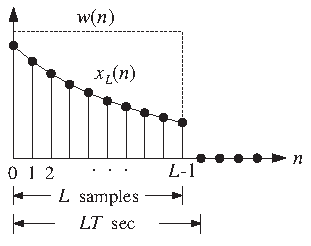
\includegraphics[height = 0.225\textwidth]{pic/rectangularWindowSamples.pdf}&&
		 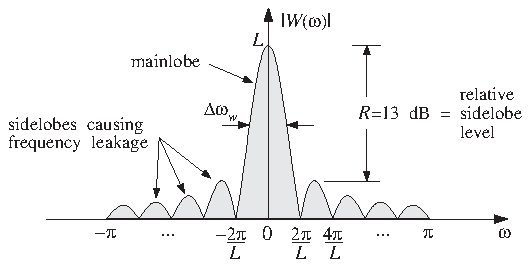
\includegraphics[height = 0.225\textwidth]{pic/rectangularWindow.pdf}\\
 		 \fcolorbox{CadetRed}{white}{$w(n) = \begin{cases}1,&0\leq n\leq L-1\\ 0,& \text{sonst}\end{cases}$} & \FT &
 		 \fcolorbox{CadetRed}{white}{$W(\omega) = \dfrac{1-\e^{-jL\omega}}{1-\e^{-j\omega}} = \dfrac{\sin(\omega L/2)}{\sin(\omega/2)}\cdot\e^{-j\omega (L-1)/2}$}\\[0.7cm]
		 \hline
		\end{tabularx} $ $\\

	\subsection{Hamming-Fenster}
		\begin{tabularx}{\textwidth}{p{0.5\textwidth}p{0.5\textwidth}}
		 \multicolumn{1}{c}{\textbf{Zeitbereich}}&\multicolumn{1}{c}{\textbf{Frequenzbereich}}\\[0.05cm]
		 \hline&\\[-0.6cm]
		 \multicolumn{1}{c}{\begin{minipage}{0.5\textwidth}
		 $\qquad\qquad$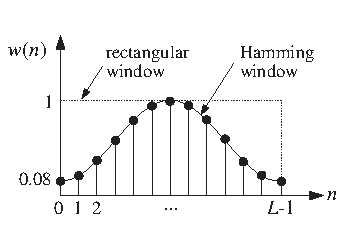
\includegraphics[width = 0.65\textwidth]{pic/hammingWindowSamples.pdf} \newline
		 \fcolorbox{CadetRed}{white}{$w(n) = \begin{cases}0.54-0.46\,\cos\left(\dfrac{2\pi n}{L-1}\right),&0\leq n\leq L-1\\ 0,& \text{sonst}\end{cases}$}
		 \end{minipage}}
		 &\multicolumn{1}{c}{\begin{minipage}{0.35\textwidth}
		 $ $\\$ $\\[0.2cm] 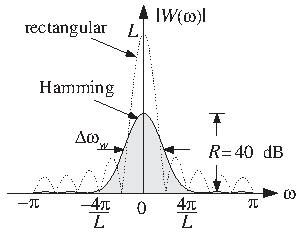
\includegraphics[width = \textwidth]{pic/hammingWindow.pdf}\end{minipage}}\\[2.9cm]
		 \hline
		\end{tabularx}
\newpage
	\subsection{Eigenschaften der Fenster-Spektren}\label{Eigenschaften der Fenster-Spektren}
		\begin{info}
		 Die Wahl des Fensters ist ein \textbf{Tradeoff} zwischen der Mainlobe-Width (Frequenzauflösung) und der Sidelobe-Suppression.
		\end{info}
		
		\begin{tabularx}{\textwidth}{|l|>{\centering\arraybackslash}X|>{\centering\arraybackslash}X|}
		 \hline&&\\[-0.3cm]
			& \textbf{Rechteck-Fenster} & \textbf{Hamming-Fenster}\\[0.1cm]
		 \hline&\multicolumn{2}{c|}{}\\[-0.3cm]
% 			Nullstellen & $\dfrac{2\pi k}{L}\quad k\neq 0$ & \\
			\textbf{Mainlobe} & \multicolumn{2}{c|}{Je grösser die Anzahl Samples $L$, desto höher und schmaler wird die Mainlobe.}\\&  \multicolumn{2}{c|}{(Die Sidelobes wachsen proportional mit.)}\\[0.1cm]
		\hline&\multicolumn{2}{c|}{}\\[-0.3cm]
			\textbf{Mainlobe-Width} &\multicolumn{2}{c|}{\fcolorbox{CadetRed}{white}{$\Delta\omega_W = c\cdot\dfrac{2\pi}{L} = c\cdot\dfrac{2\pi\Delta f_W}{f_s}$}}\\[0.6cm]
			&\multicolumn{2}{c|}{\fcolorbox{CadetRed}{white}{$\Delta f_W = c\cdot\dfrac{f_s}{L} = c\cdot\dfrac{1}{LT}= c\cdot\dfrac{1}{T_L}$} }\\[0.6cm]
			&\multicolumn{2}{c|}{$c\geq1$ }\\[0.15cm]
			& $c = 1\Rightarrow $ \textbf{Beste Frequenzauflösung} & $c = 2$\\[0.1cm]
		 \hline&&\\[-0.3cm]
			\textbf{Sidelobes} & Sind sehr gross, weil das Fenster im Zeitbereich scharf abschneidet.& Sind eher klein, weil das Fenster im Zeitbereich langsam hinein und hinaus fährt.\\[0.1cm]
		\hline&&\\[-0.3cm]
			\textbf{Sidelobe-Suppression} &\fcolorbox{CadetRed}{white}{$R = \left|\dfrac{W(\omega)}{W(0)}\right|_{\omega = 3\pi/L} \!\!\!\simeq \dfrac{2}{3\pi} \mathrel{\hat=} -13.46\db$}   & $\begin{array}{c}\text{\fcolorbox{CadetRed}{white}{$R =  -40\db$}}\\[0.2cm]\text{\textbf{$\Rightarrow$ gute Sidelobe-Suppression}}\end{array}$  \\[0.65cm]
		\hline
		\end{tabularx}$ $\\[0.2cm]

	\subsection{Frequenzauflösung}
		 Die Multiplikation des Signals $x(n)$ mit dem Fenster $w(n)$ entspricht im Frequenzbereich einer Faltung, wodurch das \textbf{Spektrum des Signals $X(\omega)$ verschmiert wird}.\\[0.2cm]
		 \fcolorbox{CadetRed}{white}{$x_L(n) = x(n) \cdot w(n)\qquad\FT\qquad X_L(\omega) = X(\omega) \ast W(\omega) = \frac{1}{2\pi}\myint{-\pi}{\pi}{X(\omega')\cdot W(\omega-\omega')}{\omega'}$}\\[0.5cm]
		 \textbf{Beispiel:}\\
		 $\begin{array}{rcl c rcl}
		 x(n) &= &A_1\,\e^{j\omega_1n} + A_2\,\e^{j\omega_2n}&\quad\FT&\quad
		 X(\omega) &= &\underline{\underline{2\pi\,A_1\,\delta(\omega-\omega_1) + 2\pi\,A_2\,\delta(\omega-\omega_2)}}\\[0.4cm]
		 x_L(n) & = & A_1\,\e^{j\omega_1n}\cdot w(n) + A_2\,\e^{j\omega_2n}\cdot w(n)&
		 \quad\FT &\quad X_L(\omega)&= &\;\;\;\;\!\myint{-\pi}{\pi}{A_1\,\delta(\omega'-\omega_1)\cdot W(\omega-\omega')}{\omega'} \\ &&&&&& + \myint{-\pi}{\pi}{A_2\,\delta(\omega'-\omega_2)\cdot W(\omega-\omega')}{\omega'}\\
		 &&&&&= & \underline{\underline{A_1\,W(\omega-\omega_1) + A_2\,W(\omega-\omega_2)}}
		 \end{array}$\\
		 \begin{minipage}{0.55\textwidth}
			$\begin{array}{ll}
			\Rightarrow& \textbf{Die Mainlobe muss schmaler sein, als der kleinste}\\ &\textbf{noch auflösbare Frequenzunterschied (Auflösung).}\\[0.2cm]
			&\text{\fcolorbox{CadetRed}{white}{$\Delta\omega \geq \Delta\omega_W = c\cdot\dfrac{2\pi}{L} = c\cdot\dfrac{2\pi\Delta f_W}{f_s}$}}\\[0.6cm]
			&\text{\fcolorbox{CadetRed}{white}{$\Delta f\geq \Delta f_W = c\cdot\dfrac{f_s}{L} = c\cdot\dfrac{1}{LT}= c\cdot\dfrac{1}{T_L}$}}\\[0.6cm]
			&\text{\fcolorbox{CadetRed}{white}{$L \geq c\cdot\dfrac{f_s}{\Delta f} = c\cdot\dfrac{2\pi}{\Delta \omega}$}}\end{array}$
		 \end{minipage}\begin{minipage}{0.05\textwidth}$ $\end{minipage}
		 \begin{minipage}{0.4\textwidth}
			$ $\\[1.5cm]
			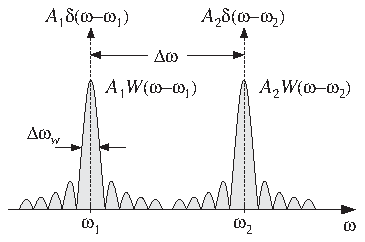
\includegraphics[width = 0.95\textwidth]{pic/frequenzaufloesung.pdf}
		 \end{minipage}
\newpage
\section{Discrete-Fourier-Transformation (DFT)}
	\begin{itemize}
	 \item Die Discrete-Time-Fourier-Transformation (DTFT) eines L-Sample langen Signals ist definiert als:\\[0.2cm]
	 \fcolorbox{CadetRed}{white}{$X(\omega) = \mysum{n=0}{L-1}{x(n)\,\e^{-j\omega n}}$}\\
	 \item Die Discrete-Fourier-Transformation (DFT) ist die DTFT, welche nur an bestimmten (diskreten) Frequenzpunkten ausgewertet wird. \\[-0.3cm]
	\end{itemize}
	
	\subsection{DFT für einzelne Frequenzen}
		\begin{itemize}
		\item Berechnung der DFT für einzelne bestimmte Frequenzen $\omega_i$ mittels der Übertragungsfunktion $H(z)$\\[0.2cm]
		\fcolorbox{CadetRed}{white}{$X(\omega_i) = \mysum{n=0}{L-1}{x(n)\,\e^{-j\omega_i n}} = \mysum{n=0}{L-1}{x(n)\,z^{-n}}|_{z = \e^{j\omega_i}} = X(z)|_{z = \e^{j\omega_i}}$}\\[0.2cm]
		$X(z) = x_0 + z^{-1}\cdot(x_1 + z^{-1}\cdot(x_2+z^{-1}\,x_3))$\\[-0.3cm]
		\end{itemize}
		
	\subsection{DFT für N-Frequenzen}
		\begin{itemize}
		 \item N-Point DFT eines L-Sample langen Signals mit N gleichmässig verteilten Frequenzpunkten.\\[0.2cm]
		\fcolorbox{CadetRed}{white}{$X(\omega_k) = \mysum{n=0}{L-1}{x(n)\,\e^{-j\omega_k n}} $}$\qquad$ mit $\quad \omega_k = \dfrac{2\pi k}{N}\qquad$ oder $\quad f_k = \dfrac{k\,f_s}{N}\qquad k = 0,1,...,N-1$\\[-0.3cm]
		\end{itemize}
		\begin{minipage}{0.7\textwidth}
		\begin{itemize}
		 \item Die N-Werte $X(\omega_k)$ können auch als Werte der z-Transformation\\ $X(z)$ auf dem Einheitskreis betrachtet werden\\[0.2cm]
		 \fcolorbox{CadetRed}{white}{$X(\omega_k) = X(z_k) = \mysum{n=0}{L-1}{x(n)\,z_k^{-n}} $}\\[0.4cm]
		 $z_k = \e^{j\omega_k} = \e^{2\pi jk/N}\qquad\quad k = 0,1,...,N-1$
		\end{itemize}
		\end{minipage}
		\begin{minipage}{0.4\textwidth} 
			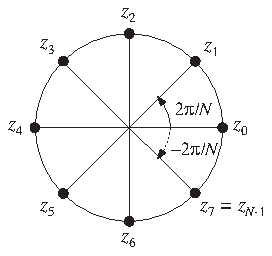
\includegraphics[width = 0.6\textwidth]{pic/dtftPeriodenKreis.pdf}
		\end{minipage}\\[-0.5cm]
		\begin{itemize}
		 \item Sie sind auch die N-ten Einheitswurzeln$\qquad$ \fcolorbox{CadetRed}{white}{$z^n = 1$}
		\end{itemize}$ $\\[-0.9cm]
		
	\subsection{Anzahl Frequenzpunkte versus Anzahl Samples}
		\begin{itemize}
		 \item \bm{$L$}: Anzahl Samples des Zeit-Signals $x(n)$
		 \item \bm{$N$}: Anzahl Samples des Frequenzspektrums $X(\omega)$
		 \item \bm{$L = N$}: Häufiger Spezialfall $\quad\Rightarrow\quad$ alles okej
		 \item \bm{$L < N$}: Zeitsequenz ist zu kurz $\quad\Rightarrow\quad$ am Ende des Signals Nullen anhängen (zero padding)
		 \item \bm{$L > N$}: Zeitsequenz ist zu lang $\quad\Rightarrow\quad$ überzählige Samples am Anfang addieren (modulo-N-wrapping\\ \hspace*{14cm}siehe Kapitel \ref{modNred})\\[-0.8cm]
		 \end{itemize}

	\subsection{Physikalische versus rechnerische Auflösung}
		\begin{minipage}{0.6\textwidth}
			\begin{tabularx}{\textwidth}{|>{\centering\arraybackslash}X|>{\centering\arraybackslash}X|}
			 \hline&\\[-0.3cm]
			 \textbf{Physikalische Auflösung} & \textbf{Rechnerische Auflösung}\\[0.1cm]
			 \hline&\\[-0.3cm]
				Frequenz-Differenz zwischen zwei noch unterscheidbaren Schwingungen aufgrund der Mainlobe-Width. & Frequenz-Differenz zwischen zwei Samples des abgetasteten Spektrums\\[0.1cm]
			 \hline&\\[-0.3cm]
				Beeinflussbar durch Anzahl Samples L des Zeit-Signals & Beeinflussbar durch Anzahl Samples N des Spektrums\\[0.1cm]
 			 \hline&\\[-0.3cm]
				\fcolorbox{CadetRed}{white}{$\Delta\omega_W = \dfrac{2\pi}{L}$}$\quad$\fcolorbox{CadetRed}{white}{$\Delta f_W = \dfrac{f_s}{L}$} & \fcolorbox{CadetRed}{white}{$\Delta\omega_{\text{bin}} = \dfrac{2\pi}{N}$}$\quad$\fcolorbox{CadetRed}{white}{$\Delta f_{\text{bin}} = \dfrac{f_s}{N}$}\\[0.5cm]
 			 \hline
			\end{tabularx}
		\end{minipage}\begin{minipage}{0.02\textwidth}$ $\end{minipage}
		\begin{minipage}{0.4\textwidth}
			\includegraphics[width = \textwidth]{pic/phyVsComRes.pdf}
		\end{minipage}
\newpage
		\textbf{Mögliche Probleme des Frequenzspektrums}\\[0.2cm]
		\begin{minipage}{0.8\textwidth}
		\begin{itemize}
		 \item Die Samples der DFT fallen nicht zwangsweise auf die Peaks der DTFT. Denn die Samples stimmen nur dann exakt, wenn $k$ (DFT Index) eine ganze Zahl ist.\\
		 $\Rightarrow$ Rechnerische Auflösung erhöhen (Anzahl Samples $N$).
		\end{itemize}
		\end{minipage}\begin{minipage}{0.05\textwidth} $ $\end{minipage}
		\begin{minipage}{0.15\textwidth}
			\fcolorbox{CadetRed}{white}{$k = N\dfrac{f}{f_s}$}
		\end{minipage}
		\begin{itemize}
		 \item Der Frequenz Bias Fehler entsteht, wenn eine Mainlobe von fremden Sidelobes gestört wird (Interferenz) und sich dadurch der Peak der Mainlobe leicht verschiebt.\\
		 $\Rightarrow$ Physikalische Auflösung erhöhen (Anzahl Samples $L$).
		\end{itemize}

	\subsection{DFT als Matrix-Multiplikation}
		\begin{itemize}
		 \item Die Diskrete-Fourier-Transformation kann auch als Matrix-Multiplikation geschrieben werden:\\[0.2cm]
		\begin{minipage}{0.3\textwidth}
			\fcolorbox{CadetRed}{white}{$\bm{X} = \text{DFT}(\bm{x}) = \bm{A\cdot x} $}
		\end{minipage}
		\begin{minipage}{0.7\textwidth}
			Matrixelement: $\;\qquad A_{kn} = \e^{-j\omega_kn} = \e^{-j2\pi kn/N} = W_N^{kn}$\\
			Twiddle-Faktor: $\qquad W_N = \e^{-j2\pi/N}$ 
		\end{minipage}$ $\\[0.3cm]
		mit $\qquad\bm{X} = \begin{bmatrix}X(\omega_0)\\X(\omega_1)\\\vdots \\ X(\omega_{N-1})\end{bmatrix} = \begin{bmatrix}X_0\\X_1\\\vdots \\ X_{N-1}\end{bmatrix}\qquad$und$\qquad\bm{x} = \begin{bmatrix}x(0)\\x(1)\\\vdots \\ x(L-1)\end{bmatrix} = \begin{bmatrix}x_0\\x_1\\\vdots \\ x_{L-1}\end{bmatrix}$\\[0.3cm]
		und$\qquad\bm{A}
% 		= \begin{bmatrix} A_{00} & A_{01} & \dots & A_{0(L-1)}\\A_{10} & A_{11} & \dots & A_{1(L-1)}\\ \vdots& \vdots& \ddots& \vdots\\A_{(N-1)0} &A_{(N-1)1} & \dots & A_{(N-1)(L-1)}\end{bmatrix}
		= \begin{bmatrix} W_N^{0\cdot0} & W_N^{0\cdot1} & \dots & W_N^{0\cdot(L-1)}\\W_N^{1\cdot0} & W_N^{1\cdot1} & \dots & W_N^{1\cdot(L-1)}\\ \vdots& \vdots& \ddots& \vdots\\W_N^{(N-1)\cdot0} & W_N^{(N-1)\cdot1} & \dots & W_N^{(N-1)\cdot(L-1)}\end{bmatrix}
		= \begin{bmatrix} 1 & 1 & \dots & 1\\1 & W_N & \dots & W_N^{(L-1)}\\ \vdots& \vdots& \ddots& \vdots\\1 & W_N^{(N-1)} & \dots & W_N^{(N-1)(L-1)}\end{bmatrix}$\\[0.2cm]
		\end{itemize}
		\begin{minipage}{0.65\textwidth}
		\begin{itemize}
			\item Die Ermittlung der Matrix $\bm{A}$ bzw. der Twiddle-Faktoren $W_N^{kn}$ geht am einfachsten über den Einheitskreis der $z$-Ebene.\\[0.2cm]
			\fcolorbox{CadetRed}{white}{$W_N^k = \e^{-j2\pi k/N} = z_{-k}$}\\[-0.1cm]
			\begin{enumerate}
			 \item Matrix Zeilenweise auffüllen
			 \item Rechts bei $1$ beginnen und im Uhrzeigersinn die Werte des Einheitskreises eintragen.
			 \item Für die nächste Zeile wiederum rechts bei $1$ beginnen und im Uhrzeigersinn die Werte des Einheitskreises eintragen jedoch die Sprunglänge um eins erhöhen.
			 \item Schritt $3.$ so oft wiederholen bis die Matrix voll ist.
			\end{enumerate}
		\end{itemize}
		\end{minipage}\begin{minipage}{0.05\textwidth} $ $ \end{minipage}
		\begin{minipage}{0.3\textwidth}
			\includegraphics[width = \textwidth]{pic/twiddleFaktor.pdf}
		\end{minipage}$ $\\

		\begin{itemize}
		 \item Beispiel für eine DFT mit $N,L = 2$ und $4$\\
		 $\begin{bmatrix}X_0\\X_1\end{bmatrix} = \begin{bmatrix}1 & 1\\ 1 & -1 \end{bmatrix}\,\begin{bmatrix}x_0\\x_1\end{bmatrix} = \begin{bmatrix}x_0+x_1\\x_0-x_1\end{bmatrix}\qquad\qquad\qquad
		 \begin{bmatrix}X_0\\X_1\\X_2\\X_3\end{bmatrix} = \begin{bmatrix}1 & 1 & 1 & 1\\ 1 & -j &  -1 & j \\ 1&-1&1&-1\\1 & j & -1 & -j\end{bmatrix}\,\begin{bmatrix}x_0\\x_1\\x_2\\x_3\end{bmatrix}$\\[-0.3cm]
		\end{itemize}

	\subsection{Modulo-N Reduktion}\label{modNred}
		\begin{itemize}
		 \item Eine Modulo-N Reduktion des Eingangssignals (Eingangsvektor $\bm{x}$) ist notwendig wenn:\\[0.2cm]
		 \fcolorbox{CadetRed}{white}{Anzahl Zeit-Samples $L\;>\;$Anzahl Frequenz-Samples $N$}
		 \item Beim wrapping-Prozess wird der Vektor $\bm{x}$ in $N-$dimensionale Subvektoren unterteilt, die dann zusammengezählt werden. Wenn $L$ kein ganzzahliges Vielfaches von $N$ ist, wird $\bm{x}$ mit Nullen aufgefüllt.\\[0.2cm]
		 \begin{minipage}{0.47\textwidth}
			\includegraphics[width = \textwidth]{pic/modNred.pdf}
		 \end{minipage}
		 \begin{minipage}{0.53\textwidth}
			$\begin{array}{lcl}\widetilde x(n) & = & x_0(n) + x_1(n) + \hdots + x_{L/N-1}(n)\\[0.2cm] &=& x(n) + x(N+n) + \hdots + x((\frac{L}{N}-1)\cdot N + n)\end{array}$\\[0.2cm]
			$\Rightarrow\quad$\fcolorbox{CadetRed}{white}{$\widetilde x(n) = \mysum{m=0}{L/N-1}{x(m\,N+n)}$}$\quad n = 0,1,...,N-1$\\[0.2cm]
			$\Rightarrow\quad$\fcolorbox{CadetRed}{white}{$\widetilde{\bm{x}} = \bm{x}_0 + \bm{x}_1 + \hdots + \bm{x}_{(L/N)-1}$}
		 \end{minipage}
\newpage
		 \item Die N-Point-DFT des originalen, $L$-langen Signals $x(n)$ und die N-Point-DFT des modulo-$N$-gewrappten Signals $\widetilde x(n)$ sind identisch.\\[-0.4cm]
		 \begin{minipage}{0.35\textwidth}
		 \fcolorbox{CadetRed}{white}{$X(\omega_k) = \widetilde X(\omega_k)\quad\Rightarrow\quad X_k = \widetilde X_k$}\\[0.2cm]
			Also gilt auch:\\[0.2cm]
			\fcolorbox{CadetRed}{white}{$\begin{array}{lcl}\bm{X}& =& \bm{A}\,\bm{x} = \begin{bmatrix}\widetilde{\bm{A}} & \widetilde{\bm{A}} & \cdots\;\;\end{bmatrix}\,\begin{bmatrix}\bm{x}_0\\\bm{x}_1\\\vdots\end{bmatrix}\\[0.8cm]& = &  \widetilde{\bm{A}}\,(\bm{x}_0+\bm{x}_1+\hdots)\; = \;\widetilde{\bm{A}}\, \widetilde{\bm{x}} \; = \;\widetilde{\bm{X}}\end{array}$}
		 \end{minipage}
		 \begin{minipage}{0.6\textwidth}
			\includegraphics[width = \textwidth]{pic/modNredBeweis.pdf}\\[1.35cm]
		 \end{minipage}$ $\\[-0.4cm]
		 Dies ist bewiesen, wenn gezeigt werden kann, dass:$\quad$\fcolorbox{CadetRed}{white}{$\bm{A} = \begin{bmatrix}\bm{\widetilde A}&\bm{\widetilde A}&\bm{\widetilde A}&\cdots\;\;\end{bmatrix}\quad$ bzw. $\quad A_{kn} = A_{k(mN+n)}$}\\[0.2cm]
		 $\underline{\underline{A_{k(mN+n)}}} = W_N^{k(mN+n)} = W_N^{kmN}\cdot W_N^{kn} = (\e^{-j2\pi/N})^{kmN}\cdot W_N^{kn} = \underbrace{\e^{-j2\pi km}}_{1}\cdot W_N^{kn} = W_N^{kn} = \underline{\underline{A_{kn}}} $
		 \item Verschiedene Signale der Länge $L$ mit der selben modulo-$N$-Reduktion haben die gleiche $N$-Point-DFT.\\[0.2cm]
		 $\bm{x}\neq \bm{y}\;\cap \;\widetilde{\bm{x}} = \widetilde{\bm{y}}\quad\Rightarrow\quad X_k = Y_k$\\[0.2cm]
		 Diese Signale haben in der z-Domäne folgende Beziehung.\\[0.2cm]
		 $F(z_k) = X(z_k) - Y(z_k) = X_k - Y_k = 0\qquad k=0,1,...,N-1$\\[0.2cm]
		 Die $N$-Nullstellen auf dem Einheitskreis sind auch Nullstellen des Differenzpolynoms $F(z)$, womit gilt:\\[0.1cm]
		 $1-z^{-N} = \myprod{k=0}{N-1}{(1-z_k\,z^{-1})}\quad\Rightarrow\quad F(z) = X(z)-Y(z) = (1-z^{-N})\,Q(z)$\\[0.2cm]
		 $\Rightarrow\quad$\fcolorbox{CadetRed}{white}{$X(z) = Y(z) + (1-z^{-N})\,Q(z)$}$\qquad$ Ordnung von $Q(z)$ ist $(L-1)-N$\\[0.2cm]
		 $\Rightarrow\quad$\textbf{Zwei Sequenzen $x(n)$ und $y(n)$, die folgende Gleichung erfüllen haben, die selbe}\\  
		 \textcolor{white}{$\Rightarrow\quad$}\textbf{N-Point-DFT!}\\[0.2cm]
		 $\Rightarrow\quad$\fcolorbox{CadetRed}{white}{$x(n) = y(n) + q(n) - q(n-N)$}$\qquad n=0,1,...,L-1$
		\end{itemize}$ $\\[-1cm]

	\subsection{Inverse-Discrete-Fourier-Transformation (IDFT)}
		$ $\\[-1.2cm]
		\begin{minipage}{0.6\textwidth}
		\begin{itemize}
			\item $\begin{array}{l}\!\!\!\text{Die Discrete-Fourier-Transformation kann geschrieben werden als:}\end{array}$\\
			$\bm{X} = \bm{A\,x} = \bm{\widetilde A\,\widetilde x}$\\[-0.3cm]
			\item $\begin{array}{l}\!\!\!\text{Damit ist die Inverse-Discrete-Fourier-Transformation folgendes:}\end{array}$\\[0.2cm]
			\fcolorbox{CadetRed}{white}{$\widetilde{\bm{x}} = \text{IDFT}(\bm{X}) = \bm{\widetilde A^{-1}\, X}$}\\[0.3cm]
			\begin{danger}
			Damit die Matrix $\bm{A}$ invertierbar ist, muss sie symetrisch sein, was bei der Matrix $\widetilde{\bm{A}}$ gegeben ist. Somit kann die IDFT nur das modulo-$N$-gewrappte Signal $\widetilde{x}$ bzw. $\widetilde{x}(n)$ rekonstruieren!
			\end{danger}\\[0.1cm]
			Dabei gilt jedoch:$\qquad$
			\fcolorbox{CadetRed}{white}{$\begin{array}{lcl}\widetilde{\bm{x}} = \bm{x}&&\text{wenn }N\geq L\\\widetilde{\bm{x}} \neq \bm{x}&&\text{wenn }N<L\\&&\Rightarrow\;\text{ Aliasing im Frequenzbereich!}\end{array}$}
		\end{itemize}
		\end{minipage}\begin{minipage}{0.05\textwidth} $ $\end{minipage}
		\begin{minipage}{0.35\textwidth}
			\includegraphics[width = \textwidth]{pic/idft.pdf}\\[3cm]	
		\end{minipage}$ $\\[-0.5cm]
		\begin{tabular}{cll}
			 $\quad\bullet\!\!\!\!$& Aufgrund der Beziehung & \fcolorbox{CadetRed}{white}{$\dfrac{1}{N}\,\widetilde{\bm{A}}\,\widetilde{\bm{A}}^\ast = \bm{I}_N\qquad\Rightarrow\qquad \widetilde{\bm{A}}^{-1} = \dfrac{1}{N}\,\widetilde{\bm{A}}^\ast$}\\[0.45cm]
			&kann die IDFT vereinfacht werden zu & \fcolorbox{CadetRed}{white}{$\widetilde{\bm{x}} = \text{IDFT}(\bm{X}) =\dfrac{1}{N}\,\widetilde{\bm{A}}^\ast \, \bm{X}$}\\[0.45cm]
			&oder mit der DFT geschrieben werden als $\qquad$& \fcolorbox{CadetRed}{white}{$\widetilde{\bm{x}} = \text{IDFT}(\bm{X}) =\dfrac{1}{N}\,\big[\text{DFT}(\bm{X}^{\ast})\big]^\ast$}\\		
		\end{tabular}
\newpage
	\subsection{DTFT/IDTFT versus DFT/IDFT}
		\begin{tabularx}{\textwidth}{|p{4.2cm}|X|X|}
		\hline&&\\[-0.25cm]
			&\textbf{DTFT/IDTFT} & \textbf{DFT/IDFT}\\[0.1cm]
		\hline&&\\[-0.25cm]
			Fourier-Transformation: &
			$\bullet\;$ $L$ Zeit-Samples\newline 
			$\bullet\;$ $\infty$ Frequenz-Samples\newline 
			$\bullet\;$ $\begin{array}{l}\\[-0.3cm]\!\!\!\text{\fcolorbox{CadetRed}{white}{$X(\omega) = \mysum{n=0}{L-1}{x(n)\,\e^{-j\omega n}}$}}\end{array}$&
			$\bullet\;$ $L$ Zeit-Samples\newline 
			$\bullet\;$ $N$ Frequenz-Samples\newline 
			$\bullet\;$ $\begin{array}{l}\\[-0.3cm]\!\!\!\text{\fcolorbox{CadetRed}{white}{$X(\omega_k) = \mysum{n=0}{L-1}{x(n)\,\e^{-j\omega_k n}}$}}\end{array}$\\[0.7cm]
		\hline&&\\[-0.25cm]
			Inverse-Fourier-Transformation: &
			$\bullet\;$ Rekonstruiert das gesamte\newline \textcolor{white}{$\bullet\;$} originale Signal $x(n)$\newline 
			$\bullet\;$ $\begin{array}{l}\\[-0.3cm]\!\!\!\text{\fcolorbox{CadetRed}{white}{$x(n) = \dfrac{1}{2\pi}\myint{0}{2\pi}{X(\omega)\,\e^{j\omega n}}{\omega}$}}\end{array}$&
			$\bullet\;$ Rekonstruiert nur das\newline \textcolor{white}{$\bullet\;$} modulo-$N$-gewrappte Signal $\widetilde{x}(n)$\newline 
			$\bullet\;$ $\begin{array}{l}\\[-0.3cm]\!\!\!\text{\fcolorbox{CadetRed}{white}{$\widetilde x(n) = \dfrac{1}{N}\mysum{k=0}{N-1}{X(\omega_k)\,\e^{j\omega_k n}}$}}\end{array}$\\[0.7cm]
		\hline&\multicolumn{2}{X|}{ }\\[-0.25cm]
			$\begin{array}{l}\!\!\!\text{IDFT als Approximation}\\\!\!\!\text{der IDTFT:}\end{array}$& 
			\multicolumn{2}{l|}{$x(n)\; = \;\dfrac{1}{2\pi}\myint{0}{2\pi}{X(\omega)\,\e^{j\omega n}}{\omega}\;\simeq\; \mysum{k=0}{N-1}{X(\omega_k)\,\e^{j\omega_k n}}\,\dfrac{\Delta\omega_{\text{bin}}}{2\pi} \; = \; \dfrac{1}{N}\mysum{k=0}{N-1}{X(\omega_k)\,\e^{j\omega_k n}}$}\\[0.4cm]
		\hline
		\end{tabularx}
	
\section{Fast-Fourier-Transformation (FFT)}
	\begin{itemize}
	 \item Die Fast-Fourier-Transformation (FFT) ist eine schnelle Implementation der Discrete-Fourier-Trans-formation (DFT), welche $N^2$ komplexe Multiplikation benötigen würde. \textbf{Somit sind die Resultate der FFT und der DFT identisch.}
	 \item Die FFT berechnet die DFT mit der ''Teile-und-Hersche'' Strategie, daher ist es von Vorteil, wenn die Anzahl Frequenz-Samples eine Zweierpotenz ist.\\[0.2cm]
	 \fcolorbox{CadetRed}{white}{$N = 2^B\qquad\Rightarrow\qquad B = \log_2(N)$}\\[-0.25cm]
	 \item Bei der FFT muss die Anzahl Zeit-Samples $L$ und die Anzahl Frequenz-Samples $N$ gleich gross sein. Ist dies nicht der Fall, so muss das Zeitsignal vorverarbeitet werden (Zero-Padding oder modulo-N-wrapping).\\[0.2cm]
	 \fcolorbox{CadetRed}{white}{$N = L$}\\[-0.2cm]
	\end{itemize}
	
	\subsection{Teile-und-Hersche Strategie}
		\begin{minipage}{0.7\textwidth}
		\begin{itemize}
		 \item Das Problem der Berechnung einer $N$-Point-DFT wird reduziert auf die Berechnung von zwei $N/2$-Point-DFTs.\\[0.2cm]
		 \fcolorbox{CadetRed}{white}{$N$ - Point - DFT$\;=\; 2\cdot \dfrac{N}{2}$ - Point - DFT$\;+\; \dfrac{N}{2}$ komplexe Multiplikationen}\\[0.2cm]
		 \item Die $N/2$-Point-DFTs wiederum in $N/4$-Point-DFTs aufteilen, usw.\\[-0.2cm]
		 \item Wenn die $N$-Point-DFT über $m$ Stufen aus $N/2^m$-Point-DFTs berechnet wird, sind $M$ komplexe Multiplikation notwendig.\\[0.2cm]
		 \fcolorbox{CadetRed}{white}{$ M\;  =\; \dfrac{N^2}{2^m} + \dfrac{N}{2}m\; =\; \underbrace{2^m\left(\dfrac{N}{2^m}\right)^2 }_{\text{DFT}} + \underbrace{2^{m-1}\dfrac{N}{2^m} +\hdots  + 4\dfrac{N}{8} + 2\dfrac{N}{4} + \dfrac{N}{2}}_{\text{Stufen-Multiplikationen}}$}\\[0.25cm]
		 \item Wenn mit $1$-Point-DFTs gestartet wird sind $m = B = \log_2(N)$ Stufen notwendig und die Berechnung der $1$-Point-DFTs entfällt, weil diese gerade sich selbst entsprechen. Damit entfällt der erste Term und es müssen nur noch die Stufen-Multiplikationen berechnet werden.\\[0.2cm]
		 \fcolorbox{CadetRed}{white}{$ M\; =\; \dfrac{N}{2}m\; =\; \dfrac{1}{2}NB\; = \;\dfrac{1}{2}N\log_2(N)$}
		\end{itemize}
		\end{minipage}\begin{minipage}{0.05\textwidth}$ $\end{minipage}
		\begin{minipage}{0.25\textwidth}
			\hspace*{0.25cm}\includegraphics[width = 0.9\textwidth]{pic/multistageDFTeinheit.pdf}\\
			\includegraphics[width = \textwidth]{pic/multistageDFT.pdf}
		\end{minipage}
\newpage
	\subsection{$\bm{N}$-Point-DFT aus zwei $\bm{N/2}$-Point-DFTs berechnen}
		\begin{itemize}
		 \item Aufsplittung der DFT $X(k)$ in zwei Terme $G(k)$ und $H(k)$ welche jeweils die geraden bzw. die ungeraden Samples der Zeit-Sequenz berücksichtigen.\\[0.2cm]
		 $\begin{array}{lclcl}
		 X(k)& =& \mysum{n=0}{N-1}{x(n)\,\e^{-j\omega_k n}}\;\; =\;\; \mysum{n=0}{N-1}{W_N^{k n}\,x(n)} &&\\[0.5cm]
		 & =& \mysum{n=0}{N/2-1}{W_N^{k(2n)}\,x(2n)} + \mysum{n=0}{N/2-1}{W_N^{k(2n+1)}\,x(2n+1)}& &\Big|\;\;\text{\fcolorbox{CadetRed}{white}{$\begin{array}{lcl}g(n)\!\!\!\! & =\!\!\!\! & x(2n)\\h(n)\!\!\!\! & =\!\!\!\! & x(2n+1)\end{array}$}}\quad n = 0,1,...,\frac{N}{2}-1 \\[0.6cm]
		 & =&\mysum{n=0}{N/2-1}{W_N^{k(2n)}\,g(n)} + \mysum{n=0}{N/2-1}{W_N^{k(2n+1)}\,h(n)} & &\Big|\;\;W_N^{2} = W_{N/2} \\[0.6cm]
		 & =& \mysum{n=0}{N/2-1}{W_{N/2}^{kn}\,g(n)} + \mysum{n=0}{N/2-1}{W_N^{k}\,W_{N/2}^{kn}\,h(n)} & &\\[0.6cm]
		 & =&\underline{\underline{G(k) + W_N^{k}\,H(k)}} & & \\[0.6cm]
		 \end{array}$\\[-0.2cm]
		 $\begin{array}{ll}\Rightarrow&\quad\text{\fcolorbox{CadetRed}{white}{$X(k) = G(k) + W_N^{k}\,H(k)$}$\qquad$ mit}\\[0.2cm]&\quad N-\text{periodisch}\\[0.1cm]&\qquad\rightarrow\quad k=0,1,...,N-1\end{array}$
		 $\qquad $\fcolorbox{CadetRed}{white}{$\begin{array}{lcl}G(k)\!\!\!\! & =\!\!\!\! & \mysum{n=0}{N/2-1}{W_{N/2}^{kn}\,g(n)}\\[0.35cm] H(k)\!\!\!\! & =\!\!\!\! & \mysum{n=0}{N/2-1}{W_{N/2}^{kn}\,h(n)}\end{array}$}$\;\;$
		  $\begin{array}{l}N/2-\text{periodisch}\\[0.1cm]\quad\rightarrow\quad k = 0,1,...,\frac{N}{2}-1\end{array}$
		 \item Um die Anzahl Multiplikation mit $W_N^k$ noch zu halbieren, wird die Eigenschaft ausgenutzt, dass $G(k)$ und $H(k)$ mit $N/2$ periodisch sind.\\[0.2cm]
		 $\begin{array}{lclcl}
		 X(k)& =& \underline{G(k) + W_N^{k}\,H(k)} &&\Big|\;\; k = 0,1,...,\frac{N}{2}-1\\[0.2cm]
		 X(k+\frac{N}{2})& =& G(k+\frac{N}{2}) + W_N^{k+N/2}\,H(k+\frac{N}{2}) &&\Big|\;\; G(k+\frac{N}{2}) = G(k)\quad\text{und}\quad H(k+\frac{N}{2}) = H(k)\\[0.2cm] 
 		 & =& G(k) + W_N^{k}\,W_N^{N/2}\,H(k) &&\Big|\;\; W_N^{N/2} = -1\\[0.2cm]
 		 & =& \underline{G(k) - W_N^{k}\,H(k)} &&
 		 \end{array}$\\[0.5cm]
		 $\Rightarrow\qquad$\fcolorbox{CadetRed}{white}{
		 $\begin{array}{lcl}
		 X(k)& =& G(k) + W_N^{k}\,H(k)\\[0.2cm]
		 X(k+\frac{N}{2})& =& G(k) - W_N^{k}\,H(k)
		 \end{array}$}$\qquad k = 0,1,...,\frac{N}{2}-1$
		 \item Somit kann eine  $N$-Point-DFT folgendermassen aus zwei $N/2$-Point-DFTs berechnet werden.\\[0.2cm]
		 \begin{minipage}{0.6\textwidth}
			\fcolorbox{CadetRed}{white}{$X(k) = 
			\begin{cases}
			\begin{bmatrix}X_0 \\ X_1\\\vdots\\X_{N/2-1}\end{bmatrix} 
			= \begin{bmatrix}G_0 \\ G_1\\\vdots\\G_{N/2-1}\end{bmatrix}
			+ \begin{bmatrix}H_0 \\ H_1\\\vdots\\H_{N/2-1}\end{bmatrix}
			\times \begin{bmatrix}W_N^0 \\ W_N^1\\\vdots\\W_N^{N/2-1}\end{bmatrix} \\
			\begin{bmatrix}X_{N/2} \\ X_{N/2+1}\\\vdots\\X_{N-1}\end{bmatrix} 
			= \begin{bmatrix}G_0 \\ G_1\\\vdots\\G_{N/2-1}\end{bmatrix}
			+ \begin{bmatrix}H_0 \\ H_1\\\vdots\\H_{N/2-1}\end{bmatrix}
			\times \begin{bmatrix}W_N^0 \\ W_N^1\\\vdots\\W_N^{N/2-1}\end{bmatrix}
			\end{cases}$}
		 \end{minipage}
		 \begin{minipage}{0.35\textwidth}
			\includegraphics[width = \textwidth]{pic/N2toNdft.pdf}
		 \end{minipage}
		 
		\end{itemize}
\newpage
	\subsection{FFT-Algorithmus}
		\begin{itemize}
		 \item Der Eingang muss in gerade und ungerade Sequenzen unterteilt werden. Dies muss so oft wiederholt werden, bis nur noch ein Element übrig bleibt.\\[0.1cm]
		 \begin{minipage}{0.4\textwidth}
			\includegraphics[width = \textwidth]{pic/andrdnungfuerFFT.pdf}
		 \end{minipage}
		 \begin{minipage}{0.55\textwidth}
			\begin{tabularx}{\textwidth}{llX}
				&$\Rightarrow\quad$ & Das richtige Anordnen der Werte für die FFT wird auch als \textbf{Bit-Reversal} bezeichnet, weil der binäre Startindex rückwärts gelesen gerade dem binären Zielindex entspricht.\\
				&&Bsp: $011\quad\rightarrow\quad 110$\\
			\end{tabularx}			
		 \end{minipage}
		 \item Wenn alle Eingangssamples richtig geordnet sind, kann der FFT-Algorithmus darauf angewendet werden.\\[0.1cm]
		 \includegraphics[width = 0.95\textwidth]{pic/FFTAlg.pdf}
		\end{itemize}

	
\section{Schnelle Faltung mit FFT}
	\begin{itemize}
	 \item Eine fundamentale Beziehung zwischen Zeit- und Frequenzbereich ist\\[0.2cm]
	 \fcolorbox{CadetRed}{white}{$\bm{y} = \bm{h}\ast\bm{ x}\qquad\Leftrightarrow\qquad Y(\omega) = H(\omega)\cdot X(\omega)$}\\[-0.3cm]
	 \item Um also die Faltung möglichst effizient berechnen zu können, kann die FFT/IFFT verwendet werden.\\[0.2cm]
	 \fcolorbox{CadetRed}{white}{$\widetilde{\bm{y}} = \widetilde{\bm{h\ast x}} =\text{IDFT}\big[\text{DFT}({\bm{h}})\cdot\text{DFT}({\bm{x}})\big]$}
	 \item Da mit der FFT/IFFT jedoch nur die \textbf{Zirkulare Faltung} (modulo-$N$-gewrappte Version) berechnet werden kann, müssen die beiden Eingangssignale $x(n)$ und $h(n)$ mit Nullen aufgefüllt werden.\\[0.2cm]
	 \begin{tabular}{|c|c|c|}
	  \hline&&\\[-0.3cm]
		Signal: & ursprüngliche Länge & Zero-Padded Länge\\[0.1cm]
	  \hline&&\\[-0.3cm]
		$\bm{x}$ & $L$ & $L_y =  L+M$\\
		$\bm{h}$ & $M+1$ (Ordnung $M$) & $L_y = L+M$\\[0.1cm]
	  \hline
	 \end{tabular}$\qquad\Rightarrow\qquad$\fcolorbox{CadetRed}{white}{$\widetilde{\bm{y}} = \bm{y}\;\;$ wenn $N\geq L_y = L+M$ }\\
	 \item Die rechnerischen Kosten dafür sind $\dfrac{3}{2}N\log_2(N) + N$ komplexe Multiplikationen
	\end{itemize}
	
	\subsection{Overlap-Add-Faltung}
			\begin{itemize}
			 \item Unendlich langes Signal $x(n)$ muss mit einem Filter $h(n)$ gefaltet werden.\\[-0.42cm]
			 \end{itemize}
		\begin{minipage}{0.55\textwidth}
			\begin{itemize}
			 \item Signal wird in $L$ lange Eingangsblöcke zerlegt, die einzeln mittels FFT und IFFT gefaltet werden.\\[-0.4cm]
			 \item Durch die Faltung entstehen $L+M$ lange Ausgangsblöcke, von welchen nur die ersten $L$ Samples direkt verwendet werden und die letzten $M$ Samples in einem Buffer $\bm{y}_\text{temp}$ zwischengespeichert werden.\\[-0.4cm]
			 \item Die Samples des Zwischenspeichers $\bm{y}_\text{temp}$ werden beim nächsten Ausgangsblock vorne addiert.
			\end{itemize}
		\end{minipage}\begin{minipage}{0.02\textwidth}$ $\end{minipage}
		\begin{minipage}{0.45\textwidth}
			\includegraphics[width = \textwidth]{pic/overlapAdd.pdf}
		\end{minipage}
\newpage
	\subsection{Overlap-Save-Faltung}
		\begin{itemize}
			 \item Unendlich langes Signal $x(n)$ muss mit einem Filter $h(n)$ gefaltet werden.
			 \item Signal wird in $L$ lange Eingangsblöcke zerlegt, welche jeweils um $M$ Samples überlappen.
			 \item Die $L$ langen Eingangsblöcke werden ohne Zero-Padding mittels FFT und IFFT gefaltet, wodurch, aufgrund der Circularen Faltung, $L$ lange Ausgangsblöcke entstehen. Bei diesen Ausgangsblöcken sind jedoch die ersten $M$ Samples falsch.
			 \item Diese falschen Samples werden jedoch verworfen, da die richtigen Samples bereits vom vorhergehenden Ausgangsblock berechnet wurden.\\[0.3cm]
			 \includegraphics[width = 0.5\textwidth]{pic/overlapSave.pdf}
		\end{itemize}

\chapter{FIR Digital Filter Design \textcolor{black}{\small S.532}}
% 
% (c) Copyright 2016 Tabea Mendez
% 
% This source is free: you can redistribute it and/or modify
% it under the terms of the GNU General Public License as published by
% the Free Software Foundation, either version 3 of the License, or
% (at your option) any later version.
% 
% This source is distributed in the hope that it will be useful,
% but WITHOUT ANY WARRANTY; without even the implied warranty of
% MERCHANTABILITY or FITNESS FOR A PARTICULAR PURPOSE.  See the
% GNU General Public License for more details.
% 
% You should have received a copy of the GNU General Public License
% along with this source.  If not, see <http://www.gnu.org/licenses/>.
%
%%%%%%%%%%%%%%%%%%%%%%%%%%%%%%%%%%%%%%%%%%%%%%%%%%%%%%%%%%%%%%%%%%%%%%%%%%%%%%


Die Fenster-Methode ist eine sehr simple Methode um FIR-Filter zu designen.
\begin{itemize}
 \item Der ideale Frequenzgang $D(\omega)$ wird in eine unendlich lange Impulsantwort $d(k)$ umgerechnet.\\[0.2cm]
 \fcolorbox{CadetRed}{white}{$D(\omega) = \mysum{k=-\infty}{\infty}{d(k)\,\e^{-j\omega k}}\qquad\Leftrightarrow\qquad d(k) = \dfrac{1}{2\pi}\myint{-\pi}{\pi}{D(\omega)\,\e^{j\omega k}}{\omega}$}\\[-1.65cm]
\end{itemize}
\begin{minipage}{0.7\textwidth}
	\begin{itemize}
	 \item Die unendlich lange Impulsantwort $d(k)$ wird symmetrisch mittels eines Fensters $w(n)$ bei $\pm M$ begrenzt. Dadurch ist die totale Anzahl Filterkoeffizienten ungerade. $\qquad$
	 \fcolorbox{CadetRed}{white}{$N = 2 M+1$}\\[0.2cm]
	 \fcolorbox{CadetRed}{white}{$\widehat D(\omega) = \mysum{k=-M}{M}{d(k)\,\e^{-j\omega k}}\qquad\Leftrightarrow\qquad d(k) = \dfrac{1}{2\pi}\myint{-\pi}{\pi}{D(\omega)\,\e^{j\omega k}}{\omega} \qquad -M\leq k \leq M$}
	\end{itemize}
\end{minipage}
\begin{minipage}{0.02\textwidth}$ $\end{minipage}
\begin{minipage}{0.28\textwidth}
	\includegraphics[width = \textwidth]{pic/FensterFIRFilter.pdf}\\[2.7cm]
\end{minipage}\\[-1.8cm]
\begin{itemize}
 \item Damit das FIR-Filter $h(n)$ kausal wird, muss die begrenzte Impuls-\\antwort $d(k)$ noch um $M$ Samples verzögert werden.\\[0.2cm]
 \fcolorbox{CadetRed}{white}{$ H(\omega) = \e^{-j\omega M} \,\widehat D(\omega) \qquad\Leftrightarrow\qquad  h(n) = d(n-M)\qquad n = 0,1,...,N-1$}\\[-0.25cm]
 \item Diese Verzögerung um $M$ Samples resultiert in einem linearphasigen Filter.
 \item Die Fenster-Methode ist sehr gut geeignet für einfache Frequenzgänge wie die folgender Filter.\\
\end{itemize}

\begin{tabularx}{\textwidth}{|>{\centering\arraybackslash}p{4.5cm}|>{\centering\arraybackslash}p{8.7cm}|X|}
 \hline&&\\[-0.3cm]
	\textbf{Filter} & \textbf{Frequenzgang $D(\omega)$ und Impulsantwort $d(k)$}& \textbf{Eigenschaften}\\[0.1cm]
 \hline&&\\[-0.2cm]
	Tiefpass &
	\multirow{2}{*}{$\begin{array}{c}\text{\fcolorbox{CadetRed}{white}{$D(\omega) = \begin{cases}1,&-\omega_c\leq\omega\leq\omega_c\\ 0,& \text{sonst}\end{cases} $}}\\[0.7cm]
	\text{\fcolorbox{CadetRed}{white}{$d(k) = \dfrac{\sin(\omega_ck)}{\pi k} $}}\end{array}$}&
	\multirow{8}{*}{$\begin{array}{l}
	\!\!\!\text{Der Frequenzgang ist:}\\\text{- reell}\\\text{- gerade}\\\text{- symmetrisch}\\[0.4cm]
	\!\!\!\text{Die Impulsantwort ist:}\\\text{- zweiseitig (akausal)}\\\text{- unendlich lang}\\\text{- reell}\\\text{- gerade}\\\text{- symmetrisch}\end{array}$}\\
	\includegraphics[width = 0.25\textwidth]{pic/tiefpass.pdf}&
	&
	\\[0.15cm]
 \cline{1-2}&&\\[-0.2cm]
	Hochpass &\multirow{2}{*}{$\begin{array}{c}\text{\fcolorbox{CadetRed}{white}{$D(\omega) = \begin{cases}0,&-\omega_c\leq\omega\leq\omega_c\\ 1,& \text{sonst}\end{cases} $}}\\[0.7cm]
	\text{\fcolorbox{CadetRed}{white}{$d(k) = \delta(k) - \dfrac{\sin(\omega_ck)}{\pi k} $}}\end{array}$}&\\
	\includegraphics[width = 0.25\textwidth]{pic/hochpass.pdf}&
	&
	\\[0.15cm]
 \cline{1-2}&&\\[-0.2cm]
	Bandpass &\multirow{2}{*}{$\begin{array}{c}\text{\fcolorbox{CadetRed}{white}{$D(\omega) = \begin{cases}1,&-\omega_b\leq\omega\leq-\omega_a\;\;\cup\;\;\omega_a\leq\omega\leq\omega_b\\ 0,& \text{sonst}\end{cases} $}}\\[0.7cm]
	\text{\fcolorbox{CadetRed}{white}{$d(k) = \dfrac{\sin(\omega_bk)-\sin(\omega_ak)}{\pi k} $}}\end{array}$}&\\
	\includegraphics[width = 0.25\textwidth]{pic/bandpass.pdf}&
	&
	\\[0.15cm]
 \cline{1-2}&&\\[-0.2cm]
	Bandsperre &
	\multirow{2}{*}{$\begin{array}{c}\text{\fcolorbox{CadetRed}{white}{$D(\omega) = \begin{cases}0,&-\omega_b\leq\omega\leq-\omega_a\;\;\cup\;\;\omega_a\leq\omega\leq\omega_b\\ 1,& \text{sonst}\end{cases} $}}\\[0.7cm]
	\text{\fcolorbox{CadetRed}{white}{$d(k) = \delta(k) - \dfrac{\sin(\omega_bk)-\sin(\omega_ak)}{\pi k} $}}\end{array}$}&\\
	\includegraphics[width = 0.25\textwidth]{pic/bandsperre.pdf}&
	&
	\\[0.15cm]
 \hline
\end{tabularx}

\begin{tabularx}{\textwidth}{|>{\centering\arraybackslash}p{4.5cm}|>{\centering\arraybackslash}p{8.7cm}|X|}
 \hline&&\\[-0.3cm]
	\textbf{Filter} & \textbf{Frequenzgang $D(\omega)$ und Impulsantwort $d(k)$}& \textbf{Eigenschaften}\\[0.1cm]
 \hline&&\\[-0.2cm]
	Differenzierer &
	\multirow{2}{*}{$\begin{array}{c}\\[-0.2cm]\text{\fcolorbox{CadetRed}{white}{$D(\omega) = j\omega$}}\\[0.5cm]
	\text{\fcolorbox{CadetRed}{white}{$d(k) = \dfrac{\cos(\pi k)}{k} -  \dfrac{\sin(\pi k)}{\pi k^2} $}}\end{array}$}&
	\multirow{4}{*}{$\begin{array}{l}
	\!\!\!\text{Der Frequenzgang ist:}\\\text{- imaginär}\\\text{- ungerade}\\\text{- antisymmetrisch}\\[0.4cm]
	\!\!\!\text{Die Impulsantwort ist:}\\\text{- zweiseitig (akausal)}\\\text{- unendlich lang}\\\text{- reell}\\\text{- ungerade}\\\text{- antisymmetrisch}\end{array}$}\\
	\includegraphics[width = 0.25\textwidth]{pic/differenzierer.pdf}&
	&
	\\[0.15cm]
 \cline{1-2}&&\\[-0.2cm]
	Hilbert-Transformator &\multirow{2}{*}{$\begin{array}{c}\\[-0.2cm]\text{\fcolorbox{CadetRed}{white}{$D(\omega) = -j\;\!\sgn(\omega)$}}\\[0.5cm]
	\text{\fcolorbox{CadetRed}{white}{$d(k) = \dfrac{1-\cos(\pi k)}{\pi k} $}}\end{array}$}&\\
	\includegraphics[width = 0.25\textwidth]{pic/hilberttransformator.pdf}&
	&
	\\[0.15cm]
 \hline
 
\end{tabularx}\\[0.1cm]
\FloatBarrier

	\section{Eigenschaft der linearen Phase}
		Wenn FIR-Filter mit der Fenster-Methode designt werden resultiert ein \textbf{linearphasiges Filter}, d.h. das Filter verzögert alle Frequenzen um genau gleich viele ($M$) Samples $\quad\Rightarrow\quad$ konstante Gruppenlaufzeit!\\[0.2cm]
		Dies kommt daher, dass ...
		\begin{itemize}
		 \item ... \textbf{symmetrische Impulsantworten keine Phase (Nullphasig) und damit keinen Delay haben.}
		 \item ... die Begrenzung einer symmetrischen/antisymmetrischen Impulsantwort die symmetrie/antisymmetrie beibehaltet und der Frequenzgang nach wie vor rein reell/imaginär ist. \\
		 \begin{danger}
		  Impulsantwort muss symmetrisch begrenzt werden, da sonst die Symmetrie und damit die\newline Linearphasigkeit aufgegeben wird.
		 \end{danger}
		 \item ... durch die eingeführte Zeitverzögerung (um das Filter kausal zu machen) aus dem nullphasigen Filter ein linearphasiges Filter wird.
		\end{itemize}$ $\\[-0.7cm]
		Die Linearphasigkeit ist in folgenden Formeln erkennbar wobei $\quad$\fcolorbox{black}{white}{$\beta(\omega) = \dfrac{1-\sgn(\widehat D(\omega))}{2} = \small\begin{cases}0,&\widehat D(\omega) > 0\\ 1,&\widehat D(\omega) < 0 \end{cases}$}\normalsize\\[-0.2cm]
		\textbf{Symmetrischer Fall (rein reell):}\\[0.2cm]
		$H(\omega)\; =\; \e^{-j\omega M} \,\widehat D(\omega) 
		\; =\; \e^{-j\omega M}\,\sgn(\widehat D(\omega))\, \big|\widehat D(\omega) \big|
		\; =\; \e^{-j\omega M}\,\e^{j\pi\beta(\omega)} \,\big|\widehat D(\omega) \big|\; =\; \underline{\e^{j(-\omega M+\pi\beta(\omega))}\,\big|\widehat D(\omega) \big|}$\\[0.2cm]
		$\;\;\Rightarrow\qquad$\fcolorbox{CadetRed}{white}{$\big|H(\omega) \big| = \big|\widehat D(\omega) \big|,\qquad \text{arg}H(\omega) \;\;=\;\; -\omega M\;\;+\underbrace{\pi\beta(\omega)}_{\text{Vorzeichenwechsel}}$}\\[0.2cm]
		\textbf{Antysymmetrischer Fall (rein imaginär):}\\[0.2cm]
		$\;\;\Rightarrow\qquad$\fcolorbox{CadetRed}{white}{$\big|H(\omega) \big| = \big|\widehat D(\omega) \big|,\qquad \text{arg}H(\omega) \;\;=\;\; -\omega M\;\;+\underbrace{\dfrac{\pi}{2}}_{\text{Offset für $j$}}+\underbrace{\pi\beta(\omega)}_{\text{Vorzeichenwechsel}}$}
	
	\section{Rechteck-Fenster}
		\begin{minipage}{0.5\textwidth}
			Das simpelste Fenster ist das Rechteck-Fenster\\[0.2cm] $\qquad$\fcolorbox{CadetRed}{white}{$w(n) =\begin{cases}1,&0\leq n\leq N-1\\0,&\text{sonst}\end{cases}$ }\\[0.4cm]
		\end{minipage}
		\begin{minipage}{0.5\textwidth}
			\includegraphics[width = 0.45\textwidth]{pic/rechteckFensterImpulsantwort.pdf}
			\includegraphics[width = 0.45\textwidth]{pic/rechteckFensterFilter.pdf}
		\end{minipage}
		Hierbei sind für das FIR-Filter-Design folgende Schritte notwendig:
		\begin{enumerate}
		 \item Wähle eine ungerade Länge $N = 2M+1$\\[-0.6cm]
		 \item Berechne die $N$ Koeffizienten von $d(k)$ mit $k = -M\leq k\leq M$. \textbf{Aufpassen bei $\bm{k=0}$!}\\[-0.6cm]
		 \item Verzögere $d(k)$ um $M$-Samples um ein kausales Filter zu erhalten $\quad $\fcolorbox{CadetRed}{white}{$h(n) = d(n-M)$}$\quad n=0,...,N-1$
		\end{enumerate}
\newpage
		
	\section{Hamming- und Hann-Fenster}
		Etwas komplexere Fenster sind das Hamming-Fenster und das Hann-Fenster.\\[0.2cm]
		\begin{minipage}{0.35\textwidth}
			Hamming-Fenster\\[0.2cm]
			\fcolorbox{CadetRed}{white}{$w(n) = 0.54-0.46\cos\left(\dfrac{2\pi n}{N-1}\right)$}\\[0.25cm]
			$n = 0,1,...,N-1$
		\end{minipage}
		\begin{minipage}{0.25\textwidth}
			\includegraphics[width = \textwidth]{pic/hammingFenster.pdf}
		\end{minipage}\begin{minipage}{0.05\textwidth}$ $\end{minipage}
		\begin{minipage}{0.25\textwidth}
			Hann-Fenster\\[0.2cm]
			\fcolorbox{CadetRed}{white}{$w(n) = 0.5-0.5\cos\left(\dfrac{2\pi n}{N-1}\right)$}\\[0.25cm]
			$n = 0,1,...,N-1$
		\end{minipage}\\
		
		\begin{minipage}{0.7\textwidth}
		Hierbei sind für das FIR-Filter-Design folgende Schritte notwendig:\\[-0.2cm]
		\begin{enumerate}
		 \item Wähle eine ungerade Länge $N = 2M+1$\\[-0.3cm]
		 \item Berechne die $N$ Koeffizienten von $d(k)$ mit $k = -M\leq k\leq M$.\\ \textbf{Aufpassen bei $\bm{k=0}$!}\\[-0.3cm]
		 \item Verzögere $d(k)$ um $M$-Samples um ein kausales Filter zu erhalten und multipliziere die verzögerte Sequenz mit dem Fenster $w(n)$\\[0.1cm] 
		 $\quad $\fcolorbox{CadetRed}{white}{$h(n) = w(n)\,d(n-M)$}$\quad n=0,...,N-1$
		\end{enumerate}
		\end{minipage}\begin{minipage}{0.05\textwidth}$ $\end{minipage}
		\begin{minipage}{0.25\textwidth}
			\includegraphics[width = \textwidth]{pic/hannFenster.pdf}\\[1.5cm]
		\end{minipage}
	\section{Frequenzgang der Filters mit dem Rechteck/Hamming-Fenster}
		\begin{itemize}
		 \item Beim Design mit der Fenster-Methode wird die verschobene Impulsantwort $d(n-M)$ mit einem Fenster multipliziert. Dies entspricht im Frequenzbereich einer Faltung.\\[0.2cm]
		 \fcolorbox{CadetRed}{white}{$h(n) = w(n)\,d(n-M)\qquad\Leftrightarrow\qquad H(\omega) = \dfrac{1}{2\pi}\myint{-\pi}{\pi}{W(\omega-\omega')\,\e^{-j\omega'M}\, D(\omega')}{\omega'}$}\\
		 \item Durch die Faltung werden die Rippel der Impulsantwort des Fensters $W(\omega)$ integriert, was zu Rippel und Überschwinger im Frequenzgang $H(\omega)$ führt.\\[0.1cm]
		 \includegraphics[width = 0.25\textwidth]{pic/spektrumRechteckFenster.pdf}$\quad$
		 \includegraphics[width = 0.56\textwidth]{pic/spektrumRechteckFenster2.pdf}\\[0.1cm]
		 \includegraphics[width = 0.25\textwidth]{pic/spektrumHammingFenster.pdf}$\quad$
		 \includegraphics[width = 0.56\textwidth]{pic/spektrumHammingFenster2.pdf}
		 \item Der Frequenzgang $H(\omega)$ ist nur durch die Anzahl Samples $N$ beeinflussbar, dabei gilt:\\[0.1cm]
		 \fcolorbox{CadetRed}{white}{$N\Uparrow\qquad\Rightarrow\qquad \text{Übergangsbandbreite } \Delta\omega\Downarrow\quad\cap\quad $schnelleres abklingen der Überschwinger}
		 \item Die Höhe der Überschwinger ist fensterabhängig und damit bei fixen Fenstern immer gleich gross\\[0.1cm]
		 \begin{tabular}{|l|c|c|}
		  \hline&&\\[-0.35cm]
			& Höhe Überschwinger & Stoppband-Dämpfung\\[0.05cm]
		  \hline&&\\[-0.35cm]
			Rechteck-Fenster & $8.9\%$ & $-20\log(0.089) =21\db$\\[0.05cm]
		  \hline&&\\[-0.35cm]
			Hamming-Fenster & $0.2\%$& $-20\log(0.002)= 54\db$\\[0.05cm]
		  \hline
		 \end{tabular}
		 \item Der Frequenzgang hat bei $\omega_c$ immer die halbe Höhe$\qquad$\fcolorbox{CadetRed}{white}{$\big|H(\omega_c)\big| = 0.5$}
		\end{itemize}	
		
	\section{Kaiser-Fenster}
		\vspace*{-0.2cm}
		\begin{minipage}{0.52\textwidth}
			Das Kaiser-Fenster ist eine Fenster-Familie welches zwei Parameter hat. Dadurch können folgende zwei Dinge eingestellt werden.\\[-0.2cm]
			\begin{itemize}
			 \item Die Übergangsbandbreite $\Delta\omega$ über die Anzahl Samples $N$\\[-0.2cm]
			 \item Die Höhe der Überschwinger bzw. die Stoppband-Dämpfung $A_{stop}$ über den Parameter $\alpha$
			\end{itemize}
		\end{minipage}\begin{minipage}{0.03\textwidth}$ $\end{minipage}
		\begin{minipage}{0.45\textwidth}
		 \includegraphics[width = \textwidth]{pic/KaiserFenster.pdf}
		\end{minipage}\\[0.1cm]
		\fcolorbox{CadetRed}{white}{$\begin{array}{lcl}w(n)&=&\dfrac{I_0(\alpha\sqrt{1-(n-M)^2/M^2})}{I_0(\alpha)}\\[0.5cm]& =& \dfrac{I_0(\alpha\sqrt{n(2M-n)}/M)}{I_0(\alpha)}\end{array}$}$\quad$
		$\begin{array}{l}n = 0,1,...,N-1\\[0.15cm] I_0(...):  \text{modifizierte Besselfunktion erster Gattung, 0-ter Ordnung.}\\[0.15cm] w(M) = 1 \;\;\text{und}\;\; w(0) = w(N-1) = 1/I_0(\alpha)\\[0.15cm] \alpha = 0\quad\Rightarrow\quad \text{Rechteck-Fenster}\end{array}$\\[0.4cm]
		\textbf{Für das FIR-Filter-Design mit Kaiser-Fenster müssen folgende Dinge gegeben sein:}\\[0.3cm]
		\begin{tabularx}{\textwidth}{>{\centering\arraybackslash}X|>{\centering\arraybackslash}X}
		 Tiefpass / Hochpass & Bandpass / Bandsperre\\[0.1cm]
		 \hline&\\[-0.3cm]
		 $\begin{array}{l}
		   \text{- Stopp- und Druchlass-Frequenz}\\[0.1cm]\qquad\text{\fcolorbox{CadetRed}{white}{$f_{stop}\;,\;f_{pass}$}}\\[0.3cm]\text{- Stopp- und Passband-Dämpfung}\\[0.1cm]\qquad\text{\fcolorbox{CadetRed}{white}{$A_{stop}\;,\;A_{pass}$}}
		  \end{array}$
		  & 
		  $\begin{array}{l}
		   \text{- Stopp- und Druchlass-Frequenz für beide Seiten}\\[0.1cm]\qquad\text{\fcolorbox{CadetRed}{white}{$f_{sa}\;,\;f_{pa}\;,\;f_{sb}\;,\;f_{pb}$}}\\[0.3cm]\text{- Stopp- und Passband-Dämpfung}\\[0.1cm]\qquad\text{\fcolorbox{CadetRed}{white}{$A_{stop}\;,\;A_{pass}$}}
		  \end{array}$\\[1.4cm]
		 \includegraphics[width = 0.45\textwidth]{pic/kaiserTPHP.pdf}
		 & \includegraphics[width = 0.45\textwidth]{pic/kaiserBPBS.pdf}\\
		\hline
		\end{tabularx}\\[0.5cm]
		\textbf{Für das FIR-Filter-Design folgende Schritte notwendig:}\\[-0.4cm]
		\begin{enumerate}
		 \item Berechnung der Übergangsbandbreite $\Delta f$\\[0.2cm]
		 \begin{tabular}{c|c}
		 Tiefpass / Hochpass & Bandpass / Bandsperre\\[0.1cm]
		 \hline&\\[-0.3cm]
		 \text{$\quad$\fcolorbox{CadetRed}{white}{$\Delta f = \big|f_{stop} - f_{pass}\big| $}$\quad$} & \text{$\quad$\fcolorbox{CadetRed}{white}{$\Delta f = \min\{\Delta f_a,\Delta f_b\} $}$\quad$\fcolorbox{black}{white}{$\Delta f_a = \big|f_{pa} - f_{sa}\big|$}$\quad$\fcolorbox{black}{white}{$\Delta f_b = \big|f_{sb} - f_{pb}\big|$}$\quad$}\\
		 \end{tabular}\\
		 \item Berechnung der Eckfrequenz $f_c$ bzw. $f_a$ und $f_b$\\[0.2cm]
		 \begin{tabular}{c|c}
		 Tiefpass / Hochpass & Bandpass / Bandsperre\\[0.1cm]
		 \hline&\\[-0.3cm]
		 \text{$\quad$\fcolorbox{CadetRed}{white}{$f_c = \dfrac{1}{2}(f_{stop} + f_{pass})$}$\quad$} & \text{$\quad\begin{array}{lll}\text{Standard-Design:}& \text{\fcolorbox{CadetRed}{white}{$f_a = f_{pa}-\frac{1}{2}\Delta f $}}&\text{\fcolorbox{CadetRed}{white}{$f_b = f_{pb}+\frac{1}{2}\Delta f $}}\\[0.25cm]\text{Alternatives-Design:}& \text{\fcolorbox{CadetRed}{white}{$f_a = f_{sa}+\frac{1}{2}\Delta f $}}&\text{\fcolorbox{CadetRed}{white}{$f_b = f_{sb}-\frac{1}{2}\Delta f $}}\\\end{array}\quad$}\\
		 \end{tabular}\\
		  \item Berechnung der digitalen Eckfrequenz $\omega_c$ bzw. $\omega_a$ und $\omega_b$\\[0.2cm]
		 \begin{tabular}{c|c}
		 Tiefpass / Hochpass & Bandpass / Bandsperre\\[0.1cm]
		 \hline&\\[-0.3cm]
		 \text{$\quad$\fcolorbox{CadetRed}{white}{$\omega_c = \dfrac{2\pi f_c}{f_s}$}$\quad$} & \text{$\quad$\fcolorbox{CadetRed}{white}{$\omega_a = \dfrac{2\pi f_a}{f_s}$}$\qquad$\fcolorbox{CadetRed}{white}{$\omega_b = \dfrac{2\pi f_b}{f_s}$}$\quad$}\\
		 \end{tabular}\\
		 \item Berechnung der Stopp- und Passband-Dämpfung $\delta_{stop}$ und $\delta_{pass}$\\[0.2cm]
		 \fcolorbox{CadetRed}{white}{$\delta_{stop} = 10^{-A_{stop}/20} \quad;\quad \delta_{pass} = \dfrac{10^{A_{pass}/20}-1}{10^{A_{pass}/20}+1}$}$\qquad$\\[0.3cm]
		 \fcolorbox{CadetRed}{white}{$A_{stop}=-20\log_{10}(\delta_{stop}) \quad;\quad A_{pass} =  20\log_{10}\left(\dfrac{1+\delta_{pass}}{1-\delta_{pass}}\right)$}\\[-0.1cm]
		 \item Berechnung der Dämpfung $\delta$ und $A$\\[0.2cm]
		 \fcolorbox{CadetRed}{white}{$ \delta = \min\{\delta_{stop},\delta_{pass}\}$}$\qquad$\fcolorbox{CadetRed}{white}{$ A = -20\log_{10}(\delta)\quad\;\quad \delta = 10^{-A/20}$}\\[-0.3cm]
		 \item Berechnung des Parameter $\alpha$ und des Filterflankenfaktors $D$, welcher anzeigt, wie viel breiter die Mainlobe des Kaiser-Fenster ist als jene des Rechteck-Fensters (Schmale Mainlobe $\quad\Rightarrow\quad$ schmale Übergangsbandbreite $\Delta f$).\\[0.2cm]
		 \fcolorbox{CadetRed}{white}{$\alpha = \begin{cases}0.1102(A-8.7),& A\geq 50\\ 0.5842(A-21)^{0.4} + 0.07886(A-21),\;\;\;& 21<A<50\\ 0,& A\leq 21\end{cases} $}$\qquad$
		 \fcolorbox{CadetRed}{white}{$D = \begin{cases}\dfrac{A-7.95}{14.36},&A>21\\[0.25cm] 0.922 ,& A\leq 21\end{cases} $}\\[-0.1cm]
		 \item Berechnung der Filterlänge $N$ mit anschliessendem Aufrunden auf die nächste ungerade Zahl und Berechnung der Verschiebung $M$.\\[0.2cm]
		 \fcolorbox{CadetRed}{white}{$\Delta f = \dfrac{Df_s}{N-1}\quad\Leftrightarrow\quad N = \dfrac{Df_s}{\Delta f}+1 $}$\qquad$\fcolorbox{CadetRed}{white}{$N = 2M+1 $}$\qquad$\fcolorbox{CadetRed}{white}{$M = \dfrac{N-1}{2}$}\\[-0.05cm]
		 \item Berechnung des Kaiser-Fensters $w(n)$ für $n=0,1,...,N-1$.
		 \item Berechnung der Impulsantwort $h(n)$ aus der Impulsantwort des gewünschten Filters $d(k)$. \\[0.2cm]
		 \fcolorbox{CadetRed}{white}{$h(n) = w(n)\,d(n-M)$}$\quad n=0,...,N-1$\\[0.2cm]
		 wobei $h(M) = \omega_c/\pi$ bzw. $h(M) = (\omega_b-\omega_a)/\pi$ ist 
		\end{enumerate}
		
		\textbf{Damit ergeben sich im Vergleich zum Rechteck- und Hamming-Fenster folgende Filter-Kennwerte}\\[0.2cm]
		\begin{tabular}{|c|c|c|c|c|}
		 \hline&&&&\\[-0.35cm]
			Fenster & $\delta$ & $A_{stop}$ & $A_{pass}$ & $D$ \\[0.05cm]
		 \hline&&&&\\[-0.35cm]
			Rechteck&	$8.9\%$ &	$21\,\db$ &		$1.55\,\db$ &	$0.92$\\
			Hamming &	$0.2\%$ &	$54\,\db$ &		$0.03\,\db$ &	$3.21$\\
			Kaiser &	variabel&	$-20\log_{10}(\delta)$ & $17.372\delta$ &$(A-7.95)/14.36$\\[0.05cm]
		 \hline
		\end{tabular}

		\subsection{Eigenschaften des Fenster-Spektrums des Kaiser-Fensters}
		Im Kapitel \ref{Eigenschaften der Fenster-Spektren} wurde der Tradeoff zwischen der Mainlobe-Width $\Delta \omega_w$ (Frequenzauflösung) und der Sidelobe-Suppression $R$ (frequency leakage) diskutiert welche jeweils fensterabhängig waren. Da das Kaiser-Fenster jedoch eine variable Form hat, variiert auch der Faktor $c$ und die Sidelobe-Suppression $R$ je nach dem, welches $\alpha$ für das Kaiser-Fenster gewählt wird.\\[0.2cm]
		\fcolorbox{CadetRed}{white}{$\Delta \omega_W = c\cdot\dfrac{2\pi}{L-1}$}$\qquad$
		\fcolorbox{CadetRed}{white}{$\Delta f_W = c\cdot\dfrac{f_s}{L-1}\quad\Leftrightarrow\quad L-1 = c\cdot \dfrac{f_s}{\Delta f_W}$}$\qquad$mit $\qquad$\fcolorbox{CadetRed}{white}{$c = \dfrac{6(R+12)}{155}$}\\[0.3cm]
		$\qquad\Rightarrow\quad$\fcolorbox{CadetRed}{white}{$\alpha = \begin{cases}0.12438(R+6.3),& 60<R<120\\0.76609(R-13.26)^{0.4} + 0.09834(R-13.26),\;\;\;& 13.26<R<60\\ 0,& R<13.26\end{cases} $}\\[0.2cm]
		Vergleich der Parameterwerte mit den anderen Fenstern$\qquad$\begin{tabular}{|c|c|c|}
		 \hline&&\\[-0.35cm]
			Fenster & $R$ & $c$ \\[0.05cm]
		 \hline&&\\[-0.3cm]
			Rechteck&	$13\,\db$ & $1$ \\
			Hamming &	$40\,\db$ & $2$\\
			Kaiser &	variabel&	$6(R+12)/155$\\[0.05cm]
		 \hline
		\end{tabular}


\chapter{IIR Digital Filter Design \textcolor{black}{\small S.563}}
% 
% (c) Copyright 2016 Tabea Mendez
% 
% This source is free: you can redistribute it and/or modify
% it under the terms of the GNU General Public License as published by
% the Free Software Foundation, either version 3 of the License, or
% (at your option) any later version.
% 
% This source is distributed in the hope that it will be useful,
% but WITHOUT ANY WARRANTY; without even the implied warranty of
% MERCHANTABILITY or FITNESS FOR A PARTICULAR PURPOSE.  See the
% GNU General Public License for more details.
% 
% You should have received a copy of the GNU General Public License
% along with this source.  If not, see <http://www.gnu.org/licenses/>.
%
%%%%%%%%%%%%%%%%%%%%%%%%%%%%%%%%%%%%%%%%%%%%%%%%%%%%%%%%%%%%%%%%%%%%%%%%%%%%%%

\vspace*{-0.5cm}
\begin{minipage}{0.4\textwidth}
 $ $\\[0.5cm]
 Ein einfacher aber indirekter Weg IIR-Filter zu designen ist mittels der Bilinear-Transformation und den Design-Methoden von analogen Filtern. Dazu sind folgende schritte notwendig:
\end{minipage}
\begin{minipage}{0.05\textwidth}$ $\end{minipage}
\begin{minipage}{0.55\textwidth}
 \includegraphics[width = \textwidth]{pic/IIRFilterDesign.pdf}
\end{minipage}\\
\begin{itemize}
 \item Die Spezifikationen des digitalen Frequenzganges mittels der Bilinear-Transformation in Spezifikationen des entsprechenden analogen Tiefpasses umwandeln.\\[0.1cm]
 \begin{tabular}{lclcl}
	digitaler Tiefpass &$\qquad\Rightarrow\qquad$& analoger Tiefpass:&$\quad$&
	\fcolorbox{CadetRed}{white}{$\Omega = g_{TP}(\omega) = \tan\left(\dfrac{\omega}{2}\right)$}\\[0.45cm]
	digitaler Hochpass &$\qquad\Rightarrow\qquad$& analoger Tiefpass:&$\quad$&
	\fcolorbox{CadetRed}{white}{$\Omega = g_{HP}(\omega) = -\cot\left(\dfrac{\omega}{2}\right)$}\\[0.45cm]
	digitaler Bandpass &$\qquad\Rightarrow\qquad$& analoger Tiefpass:&$\quad$&
	\fcolorbox{CadetRed}{white}{$\Omega = g_{BP}(\omega) = \dfrac{c-\cos(\omega)}{\sin(\omega)}$}\\[0.45cm]
	digitale Bandsperre &$\qquad\Rightarrow\qquad$& analoger Tiefpass:&$\quad$&
	\fcolorbox{CadetRed}{white}{$\Omega = g_{BS}(\omega) = \dfrac{\sin(\omega)}{\cos(\omega)-c}$}\\[0.45cm]
 \end{tabular}
 \item Den analogen Tiefpass $H_a(s)$ mit analogen Filter-Design-Methoden designen.
 \item Den analogen Tiefpass $H_a(s)$ mit der Bilinear-Transformation in das gewünschte digitale Filter $H(z)$ zurückmappen.\\[0.1cm]
 \begin{tabular}{lclcl}
	analoger Tiefpass&$\qquad\Rightarrow\qquad$& digitaler Tiefpass:&$\quad$&
	\fcolorbox{CadetRed}{white}{$s = f_{TP}(z) = \dfrac{1-z^{-1}}{1+z^{-1}}$}\\[0.45cm]
	analoger Tiefpass &$\qquad\Rightarrow\qquad$& digitaler Hochpass:&$\quad$&
	\fcolorbox{CadetRed}{white}{$s = f_{HP}(z) = \dfrac{1+z^{-1}}{1-z^{-1}}$}\\[0.45cm]
	analoger Tiefpass &$\qquad\Rightarrow\qquad$& digitaler Bandpass:&$\quad$&
	\fcolorbox{CadetRed}{white}{$s = f_{BP}(z) = \dfrac{1-2cz^{-1}+z^{-2}}{1-z^{-2}}$}\\[0.45cm]
	analoger Tiefpass &$\qquad\Rightarrow\qquad$& digitale Bandsperre:&$\quad$&
	\fcolorbox{CadetRed}{white}{$s = f_{BS}(z) = \dfrac{1-z^{-2}}{1-2cz^{-1}+z^{-2}}$}\\[0.45cm]
 \end{tabular}
 \item Damit gelten folgende Beziehungen zwischen dem analogen und digitalen Filter\\[0.2cm]
 \fcolorbox{CadetRed}{white}{$H(z) = H_a(s)\Big|_{s=f(z)}=H_a(f(z))$}$\qquad$\fcolorbox{CadetRed}{white}{$H(\omega) =H_a(s)\Big|_{s = j\Omega}= H_a(\Omega)\Big|_{\Omega=g(\omega)}=H_a(g(\omega))$}
\end{itemize}

\section{Eigenschaften der Bilinear-Transformation}
	Die Bilinear-Transformation mappt ...
	\begin{itemize}
		\item  die linke $s$-Halbebene auf das innere des Einheitskreises der $z$-Ebene (wenn $|c|\leq 1$).\\[0.15cm]
		\fcolorbox{CadetRed}{white}{stabiles analoges Filter$\;\stackrel{\mathrm{\begin{array}{l}\tiny{|c|\leq 1}\\[0.05cm]\end{array}}}\Leftrightarrow\;$stabiles digitales Filter}\\[-0.4cm]
		\item die analoge Frequenzachse $s=j\Omega$ auf\\ die digitale Frequenzachse $z=\e^{j\omega}$.\\[0.2cm]
		\fcolorbox{CadetRed}{white}{$\omega = \pm\pi\qquad \mathrel{\widehat=}\qquad\Omega =\pm\infty$}\\[-2.5cm]
	\end{itemize}
	\begin{minipage}{0.45\textwidth}$ $\end{minipage}
	\begin{minipage}{0.5\textwidth}
		\includegraphics[width = \textwidth]{pic/bilinearTrans.pdf}
	\end{minipage}
	
\section{Tiefpass-Filter und Hochpass-Filter erster Ordnung}
	\begin{itemize}
		\item Ein digitales Filter erster Ordnung hat die parametrische Form$\qquad$\fcolorbox{CadetRed}{white}{$H(z) = \dfrac{b_0+b_1\,z^{-1}}{1+a_1\,z^{-1}}$}\\[-0.15cm]
		\item Von diesem muss die erlaubte Dämpfung $A_c$ (in $\db$) bei der Grenzfrequenz $\omega_c$ spezifiziert werden.\\[0.1cm]
		\fcolorbox{CadetRed}{white}{$\big|H(\omega_c)\big|^2 = G_c^2 = 10^{-A_c/10}$}$\qquad$\fcolorbox{CadetRed}{white}{$G_c=10^{-A_c/20}$}$\qquad$\fcolorbox{CadetRed}{white}{$A_c = -10\,\log_{10}(G_c^2)= -20\,\log_{10}(G_c)$}\\[0.15cm]
		Oft$\quad$ \fcolorbox{black}{white}{$A_c = 3\,\db\quad\Rightarrow\quad G_c^2 = 1/2$}\\[-0.5cm]
		\item Die entsprechende analoge Grenzfrequenz ist$\qquad$\fcolorbox{CadetRed}{white}{$\Omega_c = g_{LP}(\omega_c)=  \tan\left(\dfrac{\omega_c}{2}\right) = \tan\left(\dfrac{\pi f_c}{f_s}\right)$}\\[0.2cm]
	\end{itemize}
	\begin{minipage}{0.48\textwidth}
		\textbf{\large{Analoges Tiefpass-Filter}}\\[0.2cm]
		\fcolorbox{CadetRed}{white}{$H_a(s)=\dfrac{\alpha}{s+\alpha}$}\\[0.2cm]
		\includegraphics[width = \textwidth]{pic/TP1ordnung.pdf}\\[-0.5cm]
		\begin{itemize}
		 \item Parameter $\alpha$\\[0.1cm]
		 $\big|H_a(\Omega_c)\big|^2 = \dfrac{\alpha^2}{|j\Omega_c+\alpha|^2} = \dfrac{\alpha^2}{\Omega_c^2+\alpha^2} = G_c^2$\\[0.2cm]
		 $\Rightarrow\quad\;$\fcolorbox{CadetRed}{white}{$\alpha = \dfrac{G_c}{\sqrt{1-G_c^2}}\,\,\Omega_c = \underbrace{\dfrac{G_c}{\sqrt{1-G_c^2}}}_{1 \text{ if } G_c^2=1/2}\,\tan\left(\dfrac{\omega_c}{2}\right)$}\\[0.2cm]
		\end{itemize}
		\textbf{\large{Digitales Tiefpass-Filter}}\\[-0.25cm]
		\begin{itemize}
		 \item Übertragungsfunktion $H(z)$\\[0.05cm]
		 $H(z) = H_a(s)\Big|_{s=f_{TP}(z)}=\dfrac{\alpha\,(1+z^{-1})}{1-z^{-1}+\alpha\,(1+z^{-1})}\!\!\!\!\!\!$\\[0.25cm]
		 $\Rightarrow\quad\;$\fcolorbox{CadetRed}{white}{$H(z) = b\,\dfrac{1+z^{-1}}{1-a\,z^{-1}}$}$\quad$\\[0.2cm]
		 \textcolor{white}{$\Rightarrow\quad\quad$}mit$\quad$\fcolorbox{black}{white}{$a = \dfrac{1-\alpha}{1+\alpha},\quad b=\dfrac{\alpha}{1+\alpha}=\dfrac{1-a}{2}$}\\[0.1cm]
		 \item Frequenzgang $H(\omega)$\\[0.2cm]
		 $H(\omega) = H_a(\Omega)\Big|_{\Omega=g_{TP}(\omega)}=\dfrac{\alpha}{\alpha + j\tan(\omega/2)}$\\[0.25cm]
		 $\Rightarrow\quad\;$\fcolorbox{CadetRed}{white}{$\big|H(\omega)\big|^2 = \dfrac{\alpha^2}{\alpha^2 + \tan^2(\omega/2)}$}
		\end{itemize}
	\end{minipage}
	\begin{minipage}{0.045\textwidth}
		\begin{tabular}{c|c}
			\\[17.5cm]
		\end{tabular}
	\end{minipage}
	\begin{minipage}{0.48\textwidth}
		\textbf{\large{Analoges Hochpass-Filter}}\\[0.2cm]
		\fcolorbox{CadetRed}{white}{$H_a(s)=\dfrac{s}{s+\alpha}$}\\[0.2cm]
		\includegraphics[width = \textwidth]{pic/HP1ordnung.pdf}\\[-0.5cm]
		\begin{itemize}
		 \item Parameter $\alpha$\\[0.1cm]
		 $\big|H_a(\Omega_c)\big|^2 = \dfrac{\Omega_c^2}{|j\Omega_c+\alpha|^2} = \dfrac{\Omega_c^2}{\Omega_c^2+\alpha^2} = G_c^2$\\[0.2cm]
		 $\Rightarrow\quad\;$\fcolorbox{CadetRed}{white}{$\alpha = \dfrac{\sqrt{1-G_c^2}}{G_c}\,\,\Omega_c = \underbrace{\dfrac{\sqrt{1-G_c^2}}{G_c}}_{1 \text{ if } G_c^2=1/2}\,\tan\left(\dfrac{\omega_c}{2}\right)$}\\[0.2cm]
		\end{itemize}
		\textbf{\large{Digitales Hochpass-Filter}}\\[-0.25cm]
		\begin{itemize}
		 \item Übertragungsfunktion $H(z)$\\[0.05cm]
		 $H(z) = H_a(s)\Big|_{s=f_{TP}(z)}=\dfrac{1-z^{-1}}{1-z^{-1}+\alpha\,(1+z^{-1})}\!\!\!\!\!\!$\\[0.25cm]
		 $\Rightarrow\quad\;$\fcolorbox{CadetRed}{white}{$H(z) = b\,\dfrac{1-z^{-1}}{1-a\,z^{-1}}$}$\quad$\\[0.2cm]
		 \textcolor{white}{$\Rightarrow\quad\quad$}mit$\quad$\fcolorbox{black}{white}{$a = \dfrac{1-\alpha}{1+\alpha},\quad b=\dfrac{1}{1+\alpha}=\dfrac{1+a}{2}$}\\[0.1cm]
		 \item Frequenzgang $H(\omega)$\\[0.2cm]
		 $H(\omega) = H_a(\Omega)\Big|_{\Omega=g_{TP}(\omega)}=\dfrac{j\tan(\omega/2)}{\alpha + j\tan(\omega/2)}$\\[0.25cm]
		 $\Rightarrow\quad\;$\fcolorbox{CadetRed}{white}{$\big|H(\omega)\big|^2 = \dfrac{\tan^2(\omega/2)}{\alpha^2 + \tan^2(\omega/2)}$}
		\end{itemize}
	\end{minipage}
	\begin{itemize}
	 \item Wenn des Hochpass- und das Tiefpass-Filter die selbe $3\,\db$-Grenzfrequenz $\omega_c$ haben, sind sie komplementäre Filter.\\[0.2cm]
	 \fcolorbox{CadetRed}{white}{$H_{TP}(z) + H_{HP}(z) = 1$}$\qquad$und$\qquad$\fcolorbox{CadetRed}{white}{$\alpha = \Omega_c = \tan\left(\dfrac{\omega_c}{2}\right)$}
	\end{itemize}
\newpage
\section{Notch-Filter und Peak-Filter zweiter Ordnung}
	\vspace*{-0.2cm}\begin{itemize}
		\item Ein digitales Filter zweiter Ordnung hat die parametrische Form$\qquad$\fcolorbox{CadetRed}{white}{$H(z) = \dfrac{b_0+b_1\,z^{-1}+b_2\,z^{-2}}{1+a_1\,z^{-1}+a_2\,z^-2}$}\\[-0.45cm]
		\item Die Spezifikations-Parameter eines Notch- bzw. Peak-Filters sind:\\[0.1cm]
		- Mittenfrequenz $\omega_0$\\[0.15cm]
		- Bandbreite \fcolorbox{CadetRed}{white}{$\Delta \omega = \omega_2-\omega_1$}\\[-0.1cm]
		- Dämpfung $G_B^2$ bei den Grenzfrequenzen $\omega_1$ und $\omega_2\quad$\fcolorbox{CadetRed}{white}{$G_B^2 = \big|H(\omega_1)\big|^2 = \big|H(\omega_2)\big|^2$}\\[-0.45cm]
		\item Die entsprechenden analogen Parameter-Spezifikationen sind:\\[0.15cm]
		\fcolorbox{CadetRed}{white}{$\Omega_0 = \tan\left(\dfrac{\omega_0}{2}\right)$}$\qquad$
		\fcolorbox{CadetRed}{white}{$\Delta\Omega = (1+\Omega_0^2)\,\tan\left(\dfrac{\Delta\omega}{2}\right)$}$\qquad$
		\fcolorbox{CadetRed}{white}{$\Omega_0^2 = \Omega_1\cdot\Omega_2$}
	\end{itemize}
	\begin{minipage}{0.48\textwidth}
		\textbf{\large{Analoges Notch-Filter}}\\[0.2cm]
		\fcolorbox{CadetRed}{white}{$H_a(s)=\dfrac{s^2 + \Omega_0^2}{s^2+\alpha s+ \Omega_0^2}$}\\[0.2cm]
		\includegraphics[width = \textwidth]{pic/Notch2ordnung.pdf}\\[-0.5cm]
		\begin{itemize}
		 \item Parameter $\alpha$\\[0.1cm]
		 $\big|H_a(\Omega_{1,2})\big|^2 = \dfrac{(\Omega_{1,2}^2-\Omega_0^2)^2}{(\Omega_{1,2}^2-\Omega_0^2)^2+\alpha^2\,\Omega_{1,2}^2} = G_B^2$\\[0.2cm]
		 $\Rightarrow\quad\;$\fcolorbox{CadetRed}{white}{$\alpha  = \underbrace{\dfrac{\sqrt{1-G_B^2}}{G_B}}_{1 \text{ if } G_B^2=1/2}\,\underbrace{(1+\Omega_0^2)\,\tan\left(\dfrac{\Delta\omega}{2}\right)}_{\Delta\Omega}$}\\[0.25cm]
		\end{itemize}
		\textbf{\large{Digitales Notch-Filter}}\\[-0.3cm]
		\begin{itemize}
		 \item Übertragungsfunktion $H(z)$\\[0.1cm]
		 $H(z) = H_a(s)\Big|_{s=f_{TP}(z)}$\\[0.2cm]
		 $\Rightarrow\quad$\fcolorbox{CadetRed}{white}{$H(z) = b\,\dfrac{1-2\cos(\omega_0)z^{-1}+z^{-2}}{1-2b\cos(\omega_0)\,z^{-1}+(2b-1)\,z^{-2}}$}$\quad$\\[0.2cm]
		 \textcolor{white}{$\Rightarrow\quad\;$}mit$\quad$\fcolorbox{black}{white}{$b=\dfrac{1}{1+\underbrace{\dfrac{\sqrt{1-G_B^2}}{G_B}\,\tan\left(\dfrac{\Delta\omega}{2}\right)}_{\beta}}$}\\[0.1cm]
		 \item Frequenzgang $H(\omega)$\\[0.2cm]
		 $H(\omega) = H_a(\Omega)\Big|_{\Omega=g_{TP}(\omega)}\\[0.2cm]
		 \hspace*{0.9cm}=\dfrac{-\tan^2(\frac{\omega}{2}) + \Omega_0^2}{-\tan^2(\frac{\omega}{2})+j\alpha\tan(\frac{\omega}{2})+ \Omega_0^2}$\\[0.25cm]
		 $\Rightarrow\quad\;$\fcolorbox{CadetRed}{white}{$\big|H(\omega)\big|^2 = \dfrac{(\tan^2(\frac{\omega}{2})-\Omega_0^2)^2}{(\tan^2(\frac{\omega}{2})-\Omega_0^2)^2+\alpha^2\,\tan^2(\frac{\omega}{2})}$}
		\end{itemize}
	\end{minipage}
	\begin{minipage}{0.045\textwidth}
		\begin{tabular}{c|c}
			\\[19.6cm]
		\end{tabular}
	\end{minipage}
	\begin{minipage}{0.48\textwidth}
		\textbf{\large{Analoges Peak-Filter}}\\[0.2cm]
		\fcolorbox{CadetRed}{white}{$H_a(s)=\dfrac{\alpha s}{s^2+\alpha s+ \Omega_0^2}$}\\[0.2cm]
		\includegraphics[width = \textwidth]{pic/Preak2ordnung.pdf}\\[-0.5cm]
		\begin{itemize}
		 \item Parameter $\alpha$\\[0.1cm]
		 $\big|H_a(\Omega_{1,2})\big|^2 = \dfrac{\alpha^2\,\Omega_{1,2}^2}{(\Omega_{1,2}^2-\Omega_0^2)^2+\alpha^2\,\Omega_{1,2}^2} = G_B^2$\\[0.2cm]
		 $\Rightarrow\quad\;$\fcolorbox{CadetRed}{white}{$\alpha = \underbrace{\dfrac{G_B}{\sqrt{1-G_B^2}}}_{1 \text{ if } G_B^2=1/2}\,\underbrace{(1+\Omega_0^2)\,\tan\left(\dfrac{\Delta\omega}{2}\right)}_{\Delta\Omega}$}\\[0.25cm]
		\end{itemize}
		\textbf{\large{Digitales Peak-Filter}}\\[-0.3cm]
		\begin{itemize}
		 \item Übertragungsfunktion $H(z)$\\[0.1cm]
		 $H(z) = H_a(s)\Big|_{s=f_{TP}(z)}$\\[0.2cm]
		 $\Rightarrow\quad$\fcolorbox{CadetRed}{white}{$H(z) = \dfrac{(1-b)\,(1-z^{-2})}{1-2b\cos(\omega_0)\,z^{-1}+(2b-1)\,z^{-2}}$}$\quad$\\[0.2cm]
		 \textcolor{white}{$\Rightarrow\quad\;$}mit$\quad$\fcolorbox{black}{white}{$b=\dfrac{1}{1+\underbrace{\dfrac{G_B}{\sqrt{1-G_B^2}}\,\tan\left(\dfrac{\Delta\omega}{2}\right)}_{\beta}}$}\\[0.1cm]
		 \item Frequenzgang $H(\omega)$\\[0.2cm]
		 $H(\omega) = H_a(\Omega)\Big|_{\Omega=g_{TP}(\omega)}\\[0.2cm]
		 \hspace*{0.9cm}=\dfrac{j\alpha\tan(\frac{\omega}{2})}{-\tan^2(\frac{\omega}{2})+j\alpha\tan(\frac{\omega}{2})+ \Omega_0^2}$\\[0.25cm]
		 $\Rightarrow\quad\;$\fcolorbox{CadetRed}{white}{$\big|H(\omega)\big|^2 = \dfrac{\alpha^2\,\tan^2(\frac{\omega}{2})}{(\tan^2(\frac{\omega}{2})-\Omega_0^2)^2+\alpha^2\,\tan^2(\frac{\omega}{2})}$}
		\end{itemize}
	\end{minipage}
\newpage

	\begin{itemize}
	 \item Das Notch-Filter hat eine Doppelte Nullstelle bei $\omega_0\quad$  \fcolorbox{CadetRed}{white}{$z_{NS} = \e^{\pm j\omega_0}$}\\
	 und das Peak-Filter hat die Nullstellen Nullstellen bei DC und bei der halben Abtast-frequenz$\quad$\fcolorbox{CadetRed}{white}{$z_{NS} = \pm 1$}
	 \item Wenn des Notch- und das Peak-Filter die selbe $3\,\db$-Mittenfrequenz $\omega_0$ und die selbe Bandbreite $\Delta\omega$ haben, sind sie komplementäre Filter. %\\[0.2cm]
	 $\quad$\fcolorbox{CadetRed}{white}{$H_{notch}(z) + H_{peak}(z) = 1$}
	\end{itemize}

	\section{Filter höherer Ordnung}
		\begin{itemize}
			\item Für das Design eines Filters höherer Ordnung müssen folgende Spezifikationen bekannt sein:\\[0.2cm]
			\begin{minipage}{0.35\textwidth}
			 \begin{itemize}
			  \item Filtertyp
			  \item Durchlassbereich $f_{pass}$
			  \item Sperrbereich $f_{stop}$
			 \end{itemize}
			\end{minipage}
			\begin{minipage}{0.5\textwidth}
			 \begin{itemize}
			  \item Passband-Dämpfung $A_{pass}$
			  \item Stoppband-Dämpfung $A_{stop}$
			 \end{itemize}
			\end{minipage}
			\item Die Pass- und Stoppband-Dämpfung können in relativen ($\db$) oder in Absoluten Werten gegeben sein.\\[0.2cm]
			\fcolorbox{CadetRed}{white}{$\begin{array}{lcl}\varepsilon_{pass}& =& \sqrt{10^{A_{pass}/10}-1}\\[0.2cm]\varepsilon_{stop}&=&\sqrt{10^{A_{stop}/10}-1}\end{array}$}$\qquad\Leftrightarrow\qquad$\fcolorbox{CadetRed}{white}{$\begin{array}{lcl}A_{pass}&=&10\log_{10}(1+\varepsilon_{pass}^2)\\[0.2cm]A_{stop}&=&10\log_{10}(1+\varepsilon_{stop}^2)\end{array}$}\\[-0.075cm]
			\item Umrechnung der digitalen Filter-Spezifikationen in die Spezifikationen des analogen Tiefpasses mittels Bilinear-Transformationen.
		\end{itemize}

		\begin{tabularx}{\textwidth}{>{\centering\arraybackslash}X|>{\centering\arraybackslash}X}
			\textbf{Tiefpass} & \textbf{Hochpass}\\[0.1cm]
			\hline&\\[-0.3cm]
			$\begin{array}{l}\text{\fcolorbox{CadetRed}{white}{$\Omega_{pass} = \tan\left(\dfrac{\omega_{pass}}{2}\right) = \tan\left(\dfrac{\pi f_{pass}}{f_s}\right)$}}\\[0.55cm]
			\text{\fcolorbox{CadetRed}{white}{$\Omega_{stop} = \tan\left(\dfrac{\omega_{stop}}{2}\right) = \tan\left(\dfrac{\pi f_{stop}}{f_s}\right)$}}\end{array}$
			& 
			$\begin{array}{l}\text{\fcolorbox{CadetRed}{white}{$\Omega_{pass} = -\cot\left(\dfrac{\omega_{pass}}{2}\right) = -\cot\left(\dfrac{\pi f_{pass}}{f_s}\right)$}}\\[0.55cm]
			\text{\fcolorbox{CadetRed}{white}{$\Omega_{stop} = -\cot\left(\dfrac{\omega_{stop}}{2}\right) = -\cot\left(\dfrac{\pi f_{stop}}{f_s}\right)$}}\end{array}$\\[1.3cm]
			\hspace*{-0.5cm}\includegraphics[width = 0.5\textwidth]{pic/ButterworthTP.pdf}
			& \includegraphics[width = 0.5\textwidth]{pic/ButterworthHP.pdf}\\
			\hline&\\[-0.3cm]
			\textbf{Bandpass} & \textbf{Bandsperre}\\[0.1cm]
			\hline&\\[-0.3cm]
			$\begin{array}{c}\text{\fcolorbox{black}{white}{$c = \cos(\omega_c)$}$\quad\Rightarrow\quad$
			\fcolorbox{CadetRed}{white}{$c = \dfrac{\sin(\omega_{pa}+\omega_{pb})}{\sin(\omega_{pa}) + \sin(\omega_{pb})}$}}\\[0.55cm]
			\text{\fcolorbox{CadetRed}{white}{$\Omega_{pass} = \left|\dfrac{c-\cos(\omega_{pb})}{\sin(\omega_{pb})}\right|$}}\\[0.6cm]
			\text{\fcolorbox{CadetRed}{white}{$\Omega_{stop} = \min\{|\Omega_{sa}|,|\Omega_{sb}|\}$}}\\[0.35cm]
			\text{mit$\quad$\fcolorbox{black}{white}{$\Omega_{sa} = \dfrac{c-\cos(\omega_{sa})}{\sin(\omega_{sa})}$}$\quad$\fcolorbox{black}{white}{$\Omega_{sb} = \dfrac{c-\cos(\omega_{sb})}{\sin(\omega_{sb})}$}}\end{array}$
			& 
			$\begin{array}{c}\text{\fcolorbox{black}{white}{$c = \cos(\omega_c)$}$\quad\Rightarrow\quad$
			\fcolorbox{CadetRed}{white}{$c = \dfrac{\sin(\omega_{pa}+\omega_{pb})}{\sin(\omega_{pa}) + \sin(\omega_{pb})}$}}\\[0.55cm]
			\text{\fcolorbox{CadetRed}{white}{$\Omega_{pass} = \left|\dfrac{\sin(\omega_{pb})}{\cos(\omega_{pb})-c}\right|$}}\\[0.6cm]
			\text{\fcolorbox{CadetRed}{white}{$\Omega_{stop} = \min\{|\Omega_{sa}|,|\Omega_{sb}|\}$}}\\[0.35cm]
			\text{mit$\quad$\fcolorbox{black}{white}{$\Omega_{sa} = \dfrac{\sin(\omega_{sa})}{\cos(\omega_{sa})-c}$}$\quad$\fcolorbox{black}{white}{$\Omega_{sb} = \dfrac{\sin(\omega_{sb})}{\cos(\omega_{sb})-c}$}}\end{array}$\\[2.5cm]
			\hspace*{-0.5cm}\includegraphics[width = 0.5\textwidth]{pic/ButterworthBP.pdf}
			& \includegraphics[width = 0.5\textwidth]{pic/ButterworthBS.pdf}\\
			\hline
		\end{tabularx}
\newpage
		\subsection{Butterworth-Filter}
			\begin{itemize}
			 \item Das analoge Tiefpass kann mit einer beliebigen Filter approximiert werden. Eine sehr weit verbreitete und simple Approximation ist das Butterworth-Filter.\\[0cm]
			 Butterworth-Filter:$\qquad$\fcolorbox{CadetRed}{white}{$\big|H(\Omega)\big|^2 = \dfrac{1}{1+\left(\dfrac{\Omega}{\Omega_0}\right)^{2N}}$}$\qquad\begin{array}{ll}\\[0.2cm]N:&\text{ Filterordnung}\\\Omega_0:&\text{ $3\,\db$ Grenzfrequenz}\end{array}$\\[0.2cm]
			 Dämpfung in $\db$:$\qquad\;\;\;$\fcolorbox{CadetRed}{white}{$A(\Omega) = -10\log_{10}\big|H(\Omega)\big|^2 = 10\log_{10}\left[1+\left(\dfrac{\Omega}{\Omega_0}\right)^{2N}\right]$}\\[-0.1cm]
			 \item Vom Butterworth-Filter ist die Ordnung $N$ zu berechnen.\\[0.075cm]
			 \fcolorbox{CadetRed}{white}{$N = \lceil N_{exakt}\rceil$}$\qquad$
			 \fcolorbox{CadetRed}{white}{$N_{exakt} = \dfrac{\ln(\varepsilon_{stop}/\varepsilon_{pass})}{\ln(\Omega_{stop}/\Omega_{pass})} = \dfrac{\ln(e)}{\ln(w)}$}$\qquad$\fcolorbox{CadetRed}{white}{$e = \dfrac{\varepsilon_{stop}}{\varepsilon_{pass}} = \sqrt{\dfrac{10^{A_{stop}/10}-1}{10^{A_{pass}/10}-1}},\quad w = \dfrac{\Omega_{stop}}{\Omega_{pass}}$}\\[-0.1cm]
			 \item Aufgrund der aufgerundeten Ordnung $N$ ist das Filter etwas ''zu gut'', d.h. dass entweder die Stoppband-Dämpfung oder die Passband-Dämpfung ''zu gut'' ist, je nach dem wie die exakte $3\,\db$ Grenzfrequenz $\Omega_0$ bestimmt wird.\\
			 $A(\Omega_{stop})>A_{stop}:\qquad\;$\fcolorbox{CadetRed}{white}{$\Omega_0 = \dfrac{\Omega_{pass}}{(10^{A_{pass}/10}-1)^{1/2N}} = \dfrac{\Omega_{pass}}{\varepsilon_{pass}^{1/N}}$}$\qquad$\\[0.2cm]
			 $A(\Omega_{pass})<A_{pass}:\qquad$\fcolorbox{CadetRed}{white}{$\Omega_0 = \dfrac{\Omega_{stop}}{(10^{A_{stop}/10}-1)^{1/2N}} = \dfrac{\Omega_{stop}}{\varepsilon_{stop}^{1/N}}$}\\
			 \item Die Übertragungsfunktion $H(s)$ kann über eine spektrale Faktorisierung ermittelt werden. Daraus geht hervor, dass alle Polstellen $s_i$ (Nullstellen des Nenner-Polynoms) auf einem Halbkreis in der linken $s$-Halbebene liegen müssen, damit das Filter stabil ist.\\[0.2cm]
			 \fcolorbox{CadetRed}{white}{$s_i = \Omega_0\,\e^{j\theta_i},\qquad \theta_i = \dfrac{\pi}{2N}(N-1+2i)$}$\qquad i=1,2,...,N$\\[0.2cm]
			 $\quad\Rightarrow\qquad$\fcolorbox{CadetRed}{white}{$H_a(s) = \myprod{i=1}{N}{\dfrac{1}{(1- \frac{1}{\Omega_0}\,\e^{-j\theta_i}\,s)}}$}\\[-3cm]
			 \hspace*{11cm}\includegraphics[width = 0.3\textwidth]{pic/ButterworthKreis.pdf}\\[-0.7cm]
			 \item Die Polstellen kommen immer in konjugiert-komplexen-Paaren vor und können daher zu Second-Order-Sections zusammengefasst werden\\[0.2cm]
			 \fcolorbox{CadetRed}{white}{$H_a(s) = H_0(s)\,H_1(s)\,H_2(s)\dots H_K(s)$}\\[0.2cm]\fcolorbox{CadetRed}{white}{$\begin{array}{lcl}H_0(s)& = &\begin{cases}\;\;\;\;\;\;1,&N=2K\\\dfrac{1}{1+s/\Omega_0},&N=2K+1\end{cases} \\[0.7cm] H_i(s) &=& \dfrac{1}{1-2\dfrac{s}{\Omega_0}\cos(\theta_i)+\dfrac{s^2}{\Omega_0^2}}\qquad i=1,2,...,K\end{array}$}\\[-0.1cm]
			 \item Der analoge Tiefpass $H_a(s)$ muss nun mit der entsprechenden Bilinear-Transformation wieder in das gewünschte digitale Filter $H(z)$ zurückgemappt werden.\\[0.1cm]
			 \begin{minipage}{0.45\textwidth}
				\begin{itemize}
				 \item Tiefpass$\qquad\overset{s=f_{TP}(z)}{\Longrightarrow}\qquad$Tiefpass\\[-0.3cm]
				 \item Tiefpass$\qquad\overset{s=f_{HP}(z)}{\Longrightarrow}\qquad$Hochpass
				\end{itemize}
			 \end{minipage}
			 \begin{minipage}{0.5\textwidth}
				\begin{itemize}
				 \item Tiefpass$\qquad\overset{s=f_{BP}(z)}{\Longrightarrow}\qquad$Bandpass\\[-0.3cm]
				 \item Tiefpass$\qquad\overset{s=f_{BS}(z)}{\Longrightarrow}\qquad$Bandsperre
				\end{itemize}
			 \end{minipage}
			\end{itemize}
\newpage
$ $\\
			\begin{tabularx}{\textwidth}{lX|lX}
			\multicolumn{2}{c|}{\textbf{\large Tiefpass}} & \multicolumn{2}{c}{\textbf{\large Hochpass}}\\[0.1cm]
			\hline&&&\\[-0.3cm]
				\multicolumn{2}{l|}{\textbf{Übertragungsfunktion $H(z)$:}} & \multicolumn{2}{l}{\textbf{Übertragungsfunktion $H(z)$:}} \\[0.15cm]
				&$H_i(z) = H_i(s)\Big|_{s=f_{TP}(z)}$ &
				&$H_i(z) = H_i(s)\Big|_{s=f_{HP}(z)}$ \\[0.4cm]
				$\Rightarrow$&\fcolorbox{CadetRed}{white}{$H_0(z) = \dfrac{G_0(1+z^{-1})}{1+a_{01}\,z^{-1}}$}&
				$\Rightarrow$&\fcolorbox{CadetRed}{white}{$H_0(z) = \dfrac{G_0(1-z^{-1})}{1+a_{01}\,z^{-1}}$}\\[0.5cm]
				&mit$\quad$\fcolorbox{black}{white}{$G_0 = \dfrac{\Omega_0}{\Omega_0+1}$}$\quad$und$\quad$\fcolorbox{black}{white}{$a_{01} = \dfrac{\Omega_0-1}{\Omega_0+1}$} &&
				mit$\quad$\fcolorbox{black}{white}{$G_0 = \dfrac{\Omega_0}{\Omega_0+1}$}$\quad$und$\quad$\fcolorbox{black}{white}{$a_{01} = -\dfrac{\Omega_0-1}{\Omega_0+1}$}\\[0.6cm]
				$\Rightarrow$&\fcolorbox{CadetRed}{white}{$H_i(z) = \dfrac{G_i(1+z^{-1})^2}{1+a_{i1}\,z^{-1}+ a_{i2}\,z^{-2}}$}&
				$\Rightarrow$&\fcolorbox{CadetRed}{white}{$H_i(z) = \dfrac{G_i(1-z^{-1})^2}{1+a_{i1}\,z^{-1}+ a_{i2}\,z^{-2}}$}\\[0.5cm]
				&mit$\,\quad$\fcolorbox{black}{white}{$G_i = \dfrac{\Omega_0^2}{1-2\,\Omega_0\cos(\theta_i)+\Omega_0^2}$}$\quad$&&
				mit$\,\quad$\fcolorbox{black}{white}{$G_i = \dfrac{\Omega_0^2}{1-2\,\Omega_0\cos(\theta_i)+\Omega_0^2}$}$\quad$\\[0.5cm]
				&und$\quad$\fcolorbox{black}{white}{$a_{i1} = \dfrac{2(\Omega_0^2-1)}{1-2\,\Omega_0\cos(\theta_i)+\Omega_0^2}$} &&
				und$\quad$\fcolorbox{black}{white}{$a_{i1} = -\dfrac{2(\Omega_0^2-1)}{1-2\,\Omega_0\cos(\theta_i)+\Omega_0^2}$}\\[0.5cm]
				&und$\quad$\fcolorbox{black}{white}{$a_{i2} = \dfrac{1+2\,\Omega_0\cos(\theta_i)+\Omega_0^2}{1-2\,\Omega_0\cos(\theta_i)+\Omega_0^2}$} &&
				und$\quad$\fcolorbox{black}{white}{$a_{i2} = \dfrac{1+2\,\Omega_0\cos(\theta_i)+\Omega_0^2}{1-2\,\Omega_0\cos(\theta_i)+\Omega_0^2}$}\\[0.6cm]
				$\Rightarrow$&\fcolorbox{CadetRed}{white}{$H(z) = H_0(z)\,H_1(z)\,H_2(z)\dots H_K(z)$}&
				$\Rightarrow$&\fcolorbox{CadetRed}{white}{$H(z) = H_0(z)\,H_1(z)\,H_2(z)\dots H_K(z)$}\\[0.5cm]
				\multicolumn{2}{l|}{\textbf{Frequenzgang $H(\omega)$:}} & \multicolumn{2}{l}{\textbf{Frequenzgang $H(\omega)$:}} \\[0.15cm]
				&$H(\omega) = H_a(\Omega)\Big|_{\Omega=g_{TP}(\omega)}$ & & $H(\omega) = H_a(\Omega)\Big|_{\Omega=g_{HP}(\omega)}$\\[0.4cm]
				$\Rightarrow$&\fcolorbox{CadetRed}{white}{$\big|H(\omega)\big|^2 = \dfrac{1}{1+(\tan(\frac{\omega}{2})/\Omega_0)^{2N}}$}&
				$\Rightarrow$&\fcolorbox{CadetRed}{white}{$\big|H(\omega)\big|^2 = \dfrac{1}{1+(\cot(\frac{\omega}{2})/\Omega_0)^{2N}}$}\\[0.8cm]
				\multicolumn{2}{l|}{\textbf{3$\,\db$ Grenzfrequenz $\omega_0$:}} & \multicolumn{2}{l}{\textbf{3$\,\db$ Grenzfrequenz $\omega_0$:}} \\[0.15cm]
				&\fcolorbox{CadetRed}{white}{$\omega_0 = 2\,\arctan(\Omega_0)$}$\quad$\fcolorbox{CadetRed}{white}{$f_0 = \dfrac{f_s}{\pi}\,\arctan(\Omega_0)$}&&\fcolorbox{CadetRed}{white}{$\omega_0 = 2\,\arctan\left(\dfrac{1}{\Omega_0}\right)$}$\quad$\fcolorbox{CadetRed}{white}{$f_0 = \dfrac{f_s}{\pi}\,\arctan\left(\dfrac{1}{\Omega_0}\right)$}\\[0.7cm]
				\hline
			\end{tabularx}
\newpage
$ $\\
			\begin{tabularx}{\textwidth}{lX|lX}			
				\multicolumn{2}{c|}{\textbf{\large Bandpass}} & \multicolumn{2}{c}{\textbf{\large Bandsperre}}\\[0.1cm]
			\hline&&&\\[-0.3cm]
				\multicolumn{2}{l|}{\textbf{Übertragungsfunktion $H(z)$:}} & \multicolumn{2}{l}{\textbf{Übertragungsfunktion $H(z)$:}} \\[0.15cm]
				&$H_i(z) = H_i(s)\Big|_{s=f_{BP}(z)}$ &
				&$H_i(z) = H_i(s)\Big|_{s=f_{BS}(z)}$ \\[0.4cm]
				$\Rightarrow$&\fcolorbox{CadetRed}{white}{$H_0(z) = \dfrac{G_0(1-z^{-2})}{1+a_{01}\,z^{-1}+a_{02}\,z^{-2}}$}&
				$\Rightarrow$&\fcolorbox{CadetRed}{white}{$H_0(z) = \dfrac{G_0(1-2c\,z^{-1}+z^{-2})}{1+a_{01}\,z^{-1}+a_{02}\,z^{-2}}$}\\[0.5cm]
				&mit$\quad$\fcolorbox{black}{white}{$G_0 = \dfrac{\Omega_0}{1+\Omega_0}$}$\quad$und$\quad$\fcolorbox{black}{white}{$a_{01} = -\dfrac{2c}{1+\Omega_0}$} &&
				mit$\quad$\fcolorbox{black}{white}{$G_0 = \dfrac{\Omega_0}{1+\Omega_0}$}$\quad$und$\quad$\fcolorbox{black}{white}{$a_{01} = -\dfrac{2c\,\Omega_0}{1+\Omega_0}$}\\[0.6cm]
				&und$\quad$\fcolorbox{black}{white}{$a_{02} = \dfrac{1-\Omega_0}{1+\Omega_0}$} &&
				und$\quad$\fcolorbox{black}{white}{$a_{02} = -\dfrac{1-\Omega_0}{1+\Omega_0}$}\\[0.6cm]
				$\Rightarrow$&\fcolorbox{CadetRed}{white}{$H_i(z)\! =\! \dfrac{G_i(1-z^{-2})^2}{1+a_{i1}z^{-1}+ a_{i2}z^{-2}+ a_{i3}z^{-3}+ a_{i4}z^{-4}}$}&
				$\Rightarrow$&\fcolorbox{CadetRed}{white}{$H_i(z)\! =\! \dfrac{G_i(1-2c\,z^{-1}+z^{-2})^2}{1+a_{i1}z^{-1}+ a_{i2}z^{-2}+ a_{i3}z^{-3}+ a_{i4}z^{-4}}$}\\[0.5cm]
				&mit$\,\quad$\fcolorbox{black}{white}{$G_i = \dfrac{\Omega_0^2}{1-2\,\Omega_0\cos(\theta_i)+\Omega_0^2}$}$\quad$&&
				mit$\,\quad$\fcolorbox{black}{white}{$G_i = \dfrac{\Omega_0^2}{1-2\,\Omega_0\cos(\theta_i)+\Omega_0^2}$}\\[0.5cm]
				&und$\quad$\fcolorbox{black}{white}{$a_{i1} = \dfrac{4c\,(\Omega_0\cos(\theta_i)-1)}{1-2\,\Omega_0\cos(\theta_i)+\Omega_0^2}$} &&
				und$\quad$\fcolorbox{black}{white}{$a_{i1} = \dfrac{4c\,\Omega_0\,(\cos(\theta_i)-\Omega_0)}{1-2\,\Omega_0\cos(\theta_i)+\Omega_0^2}$}\\[0.5cm]
				&und$\quad$\fcolorbox{black}{white}{$a_{i2} = \dfrac{2\,(2c^2+1-\Omega_0^2)}{1-2\,\Omega_0\cos(\theta_i)+\Omega_0^2}$} &&
				und$\quad$\fcolorbox{black}{white}{$a_{i2} = \dfrac{2\,(2c^2\,\Omega_0^2+\Omega_0^2-1)}{1-2\,\Omega_0\cos(\theta_i)+\Omega_0^2}$}\\[0.5cm]
				&und$\quad$\fcolorbox{black}{white}{$a_{i3} = -\dfrac{4c\,(\Omega_0\cos(\theta_i)+1)}{1-2\,\Omega_0\cos(\theta_i)+\Omega_0^2}$} &&
				und$\quad$\fcolorbox{black}{white}{$a_{i3} = -\dfrac{4c\,\Omega_0\,(\cos(\theta_i)+\Omega_0)}{1-2\,\Omega_0\cos(\theta_i)+\Omega_0^2}$}\\[0.5cm]
				&und$\quad$\fcolorbox{black}{white}{$a_{i4} = \dfrac{1+2\,\Omega_0\cos(\theta_i)+\Omega_0^2}{1-2\,\Omega_0\cos(\theta_i)+\Omega_0^2}$} &&
				und$\quad$\fcolorbox{black}{white}{$a_{i4} = \dfrac{1+2\,\Omega_0\cos(\theta_i)+\Omega_0^2}{1-2\,\Omega_0\cos(\theta_i)+\Omega_0^2}$}\\[0.6cm]
				$\Rightarrow$&\fcolorbox{CadetRed}{white}{$H(z) = H_0(z)\,H_1(z)\,H_2(z)\dots H_K(z)$}&
				$\Rightarrow$&\fcolorbox{CadetRed}{white}{$H(z) = H_0(z)\,H_1(z)\,H_2(z)\dots H_K(z)$}\\[0.5cm]
				\multicolumn{2}{l|}{\textbf{Frequenzgang $H(\omega)$:}} & \multicolumn{2}{l}{\textbf{Frequenzgang $H(\omega)$:}} \\[0.15cm]
				&$H(\omega) = H_a(\Omega)\Big|_{\Omega=g_{BP}(\omega)}$ & &$H(\omega) = H_a(\Omega)\Big|_{\Omega=g_{BS}(\omega)}$\\[0.4cm]
				$\Rightarrow$&\fcolorbox{CadetRed}{white}{$\big|H(\omega)\big|^2 = \dfrac{1}{1+\left(\dfrac{(c-\cos(\omega))/\sin(\omega)}{\Omega_0}\right)^{2N}}$}&
				$\Rightarrow$&\fcolorbox{CadetRed}{white}{$\big|H(\omega)\big|^2 = \dfrac{1}{1+\left(\dfrac{\sin(\omega)/(\cos(\omega)-c)}{\Omega_0}\right)^{2N}}$}\\[1.4cm]
				\multicolumn{2}{l|}{\textbf{3$\,\db$ Grenzfrequenzen $\omega_{0a}$ und $\omega_{0b}$:}} & \multicolumn{2}{l}{\textbf{3$\,\db$ Grenzfrequenzen $\omega_{0a}$ und $\omega_{0b}$:}} \\[0.15cm]
				&\fcolorbox{CadetRed}{white}{$\tan\!\left(\dfrac{\omega_{0a}}{2}\right) \!=\! \tan\!\left(\dfrac{\pi f_{0a}}{f_s}\right) \!=\! \dfrac{\sqrt{\Omega_0^2+1-c^2}-\Omega_0}{1+c}$}&&
				\fcolorbox{CadetRed}{white}{$\tan\!\left(\dfrac{\omega_{0a}}{2}\right) \!=\! \tan\!\left(\dfrac{\pi f_{0a}}{f_s}\right) \!=\! \dfrac{\sqrt{1+\Omega_0^2\,(1-c^2)}-1}{\Omega_0(1+c)}$}\\[0.6cm]
				&\fcolorbox{CadetRed}{white}{$\tan\!\left(\dfrac{\omega_{0b}}{2}\right) \!=\! \tan\!\left(\dfrac{\pi f_{0b}}{f_s}\right) \!=\! \dfrac{\sqrt{\Omega_0^2+1-c^2}+\Omega_0}{1+c}$}&&
				\fcolorbox{CadetRed}{white}{$\tan\!\left(\dfrac{\omega_{0b}}{2}\right) \!=\! \tan\!\left(\dfrac{\pi f_{0b}}{f_s}\right) \!=\! \dfrac{\sqrt{1+\Omega_0^2\,(1-c^2)}+1}{\Omega_0(1+c)}$}\\[0.7cm]
			\hline
			\end{tabularx}

\chapter{Interpolation, Dezimierung und Oversampling \textcolor{black}{\small S.632}}
% 
% (c) Copyright 2016 Tabea Mendez
% 
% This source is free: you can redistribute it and/or modify
% it under the terms of the GNU General Public License as published by
% the Free Software Foundation, either version 3 of the License, or
% (at your option) any later version.
% 
% This source is distributed in the hope that it will be useful,
% but WITHOUT ANY WARRANTY; without even the implied warranty of
% MERCHANTABILITY or FITNESS FOR A PARTICULAR PURPOSE.  See the
% GNU General Public License for more details.
% 
% You should have received a copy of the GNU General Public License
% along with this source.  If not, see <http://www.gnu.org/licenses/>.
%
%%%%%%%%%%%%%%%%%%%%%%%%%%%%%%%%%%%%%%%%%%%%%%%%%%%%%%%%%%%%%%%%%%%%%%%%%%%%%%

\section{Interpolation und Oversampling}
	\begin{goal}
	  Ein Upsampling mit anschliessender Interpolation wird oft gemacht, um die Anforderungen an das analoge Anti-Image-Filter (D/A) zu verringern. Stattdessen wird jedoch ein digitales Interpolations-Filter mit hohen Anforderungen gebraucht.
	\end{goal}

	\subsection{Schritte im Zeitbereich}
		\hspace*{1cm}\includegraphics[width = 0.75\textwidth]{pic/Upsampler.pdf}
		\begin{itemize}
		  \item Digitales Signal $x(n)$ um den Faktor $L$ upsamplen, wobei alle neuen Samples auf Null gesetzt werden.\\[0.2cm]
		  \fcolorbox{CadetRed}{white}{$x_{up}(n') = \begin{cases}x(n),&\text{wenn }n' = n\, L\\ 0,&\text{sonst}\end{cases}$}$\qquad$mit$\qquad$\fcolorbox{CadetRed}{white}{$n' = n\,L + i$}$\quad i=0,1,2,...,L-1$\\
		  \item Das Upgesampletes Signal $x_{up}(n')$ wird durch ein\\FIR-Interpolations-Filter gelassen, welches die neuen\\ Samples auf den richtigen Wert setzt.\\[-1.35cm]
		  \hspace*{10.2cm}\fcolorbox{CadetRed}{white}{$y_{up}(n') = \mysum{k'}{\textcolor{white}{ds}}{h(k')\,x_{up}(n'-k')}$}\\[-0.1cm]
		  \item Es resultiert ein Signal $y_{up}(n')$ welches eine höhere Taktrate hat.$\qquad$
		  \fcolorbox{CadetRed}{white}{$f_s' = L\cdot f_s\qquad\Leftrightarrow\qquad T' = \dfrac{T}{L}$}\\[-0.4cm]
		\end{itemize}
		
	\subsection{Schritte im Frequenzbereich}
		\begin{itemize}
		  \item Spektrum $X(f)$ des langsam\\ abgetasteten Signal $x(n)$.\\[-1.5cm]
			\begin{minipage}{0.3\textwidth}$ $\end{minipage}
			\begin{minipage}{0.7\textwidth}
			\begin{tikzpicture}[>=latex, scale=0.9]
				\draw[->][line width=0.75](0,-0.2)node[below]{\small$0$}--(0,2.2)node[right]{\small$X(f)$};
				\draw[->][line width=0.75](-6,0)--(6,0)node[below]{\small$f$};

				\draw[line width=0.75](1.2,0.2)--(1.2,-0.2)node[below]{\small$f_s$};
				\draw[line width=0.75](-1.2,0.2)--(-1.2,-0.2)node[below]{\small$-f_s$};
				\draw[line width=0.75](2*1.2,0.2)--(2*1.2,-0.2)node[below]{\small$2f_s$};
				\draw[line width=0.75](-2*1.2,0.2)--(-2*1.2,-0.2)node[below]{\small$-2f_s$};
				\draw[line width=0.75](3*1.2,0.2)--(3*1.2,-0.2)node[below=5pt]{\small$\dots$};
				\draw[line width=0.75](-3*1.2,0.2)--(-3*1.2,-0.2)node[below=5pt]{\small$\dots$};
				\draw[line width=0.75](4*1.2,0.2)--(4*1.2,-0.2)node[below]{\small$Lf_s$};
				\draw[line width=0.75](-4*1.2,0.2)--(-4*1.2,-0.2)node[below]{\small$-Lf_s$};
				

				\foreach \i in {-4,...,4}
				{
					\draw[CadetRed, line width=1](1.2*\i,0)++(-0.6,0)--++(0.25,1.3)--node[above]{}++(0.7,0)--++(0.25,-1.3);
				}
				\draw[blueT, line width=1](0,0)++(-0.6,0)--++(0.25,1.3)--node[above left]{\small $f_s\,X_a(f)$}++(0.7,0)--++(0.25,-1.3);

				\draw[line width=2, blueT](-0.6,0)--(0.6,-0);
				\draw[line width=0.75, blueT](-0.6,0.2)--(-0.6,-0.9);
				\draw[line width=0.75, blueT](0.6,0.2)--(0.6,-0.9);
				\draw[line width=0.75, blueT,<->](-0.6,-0.8)--node[below]{\footnotesize Nyquistintervall}(0.6,-0.8);


				\begin{scope}[shift={(6,0)}]
					\draw[CadetRed, line width=1,fill](0,0.65)circle(1pt);
					\draw[CadetRed, line width=1,fill](0.25,0.65)circle(1pt);
					\draw[CadetRed, line width=1,fill](-0.25,0.65)circle(1pt);
				\end{scope}
				\begin{scope}[shift={(-6,0)}]
					\draw[CadetRed, line width=1,fill](0,0.65)circle(1pt);
					\draw[CadetRed, line width=1,fill](0.25,0.65)circle(1pt);
					\draw[CadetRed, line width=1,fill](-0.25,0.65)circle(1pt);
				\end{scope}
			\end{tikzpicture}	
			\end{minipage}\\[-0.4cm]
		  \item Durch das Upsamplen um den Faktor $L$ verändert sich\\ das Spektrum $X(f)$ des digitalen Signals $x(n)$\\ nicht, da die neuen Samples\\ alle Null sind. Es ändert nur\\ die Samplingfrequenz $f_s\rightarrow f_s'$\\[0.2cm]
		  $\;\Rightarrow\qquad$\fcolorbox{CadetRed}{white}{$X_{up}(f) = X(f)$}\\[-3.1cm]
			\begin{minipage}{0.3\textwidth}$ $\end{minipage}
			\begin{minipage}{0.7\textwidth}
			\begin{tikzpicture}[>=latex, scale=0.9]
				\draw[->][line width=0.75](0,-0.2)node[below]{\small$0$}--(0,2.2)node[right]{\small$X_{up}(f) = X(f)$};
				\draw[->][line width=0.75](-6,0)--(6,0)node[below]{\small$f$};

				\foreach \i in {-4,...,4}
				{
					\draw[CadetRed, line width=1](1.2*\i,0)++(-0.6,0)--++(0.25,1.3)--node[above]{}++(0.7,0)--++(0.25,-1.3);
				}
				\draw[blueT, line width=1](0,0)++(-0.6,0)--++(0.25,1.3)--node[above left]{\small $f_s\,X_a(f)$}++(0.7,0)--++(0.25,-1.3);

				\draw[line width=2, blueT](-0.6*4,0)--(0.6*4,-0);
				\draw[line width=0.75, blueT](-0.6*4,0.2)--(-0.6*4,-1.25);
				\draw[line width=0.75, blueT](0.6*4,0.2)--(0.6*4,-1.25);
				\draw[line width=0.75, blueT,<->](-0.6*4,-1.1)--node[fill=white]{\footnotesize Nyquistintervall}(0.6*4,-1.1);

		% 		\draw[line width=0.75](1.2*0.5,0.2)--(1.2*0.5,-0.2)node[below]{\small$f_s'/8$};
		% 		\draw[line width=0.75](-1.2*0.5,0.2)--(-1.2*0.5,-0.2)node[below]{\small$-f_s'/8\;\;\;\;$};		
				\draw[line width=0.75](1.2,0.2)--(1.2,-0.2)node[below]{\small$f_s'/L$};
				\draw[line width=0.75](-1.2,0.2)--(-1.2,-0.2)node[below]{\small$-f_s'/L$};
				\draw[line width=0.75](2*1.2,0.2)--(2*1.2,-0.2)node[below,fill=white]{\small$f_s'/2$};
				\draw[line width=0.75](-2*1.2,0.2)--(-2*1.2,-0.2)node[below,fill=white]{\small$-f_s'/2$};
				\draw[line width=0.75](3*1.2,0.2)--(3*1.2,-0.2)node[below=5pt]{\small$\dots$};
				\draw[line width=0.75](-3*1.2,0.2)--(-3*1.2,-0.2)node[below=5pt]{\small$ \dots$};
				\draw[line width=0.75](4*1.2,0.2)--(4*1.2,-0.2)node[below]{\small$f_s'$};
				\draw[line width=0.75](-4*1.2,0.2)--(-4*1.2,-0.2)node[below]{\small$-f_s'$};

				\begin{scope}[shift={(6,0)}]
					\draw[CadetRed, line width=1,fill](0,0.65)circle(1pt);
					\draw[CadetRed, line width=1,fill](0.25,0.65)circle(1pt);
					\draw[CadetRed, line width=1,fill](-0.25,0.65)circle(1pt);
				\end{scope}
				\begin{scope}[shift={(-6,0)}]
					\draw[CadetRed, line width=1,fill](0,0.65)circle(1pt);
					\draw[CadetRed, line width=1,fill](0.25,0.65)circle(1pt);
					\draw[CadetRed, line width=1,fill](-0.25,0.65)circle(1pt);
				\end{scope}
			\end{tikzpicture}
			\end{minipage}\\[-0.3cm]
		  \item Eine perfekte Interpolation im Zeitbereich entspricht\\ einem idealen digitalen Tiefpassfilter $D(f)$,\\ welches die spektralen Kopien\\ des Original-Sprektrums im\\ Nyquistband auslöscht.\\[-2.3cm]
			\begin{minipage}{0.3\textwidth}$ $\end{minipage}
			\begin{minipage}{0.7\textwidth}
			\begin{tikzpicture}[>=latex, scale=0.9]
				\draw[->][line width=0.75](0,-0.2)node[below]{\small$0$}--(0,2.4)node[right]{\small$Y_{up}(f)$};
				\draw[->][line width=0.75](-6,0)--(6,0)node[below]{\small$f$};

				\foreach \i in {-3,-2,-1,1,2,3}
				{
					\draw[CadetRed, line width=1,dashed](1.2*\i,0)++(-0.6,0)--++(0.25,1.3)--node[above]{}++(0.7,0)--++(0.25,-1.3);
				}
				\foreach \i in {-4,0,4}
				{
					\draw[CadetRed, line width=1](1.2*\i,0)++(-0.6,0)--++(0.25,1.3)--node[above]{}++(0.7,0)--++(0.25,-1.3);
				}

				\draw[blueT, line width=1](0,0)++(-0.6,0)--++(0.25,1.3)--node[above left,yshift=2pt]{\small $f_s\,X_a(f)$}node[above right,yshift=2pt,gray]{\small $D(f)$}++(0.7,0)--++(0.25,-1.3);


				\draw[gray, line width=1.25](-1.2*4.5-0.3,0.1)--++(0.3,0)--++(0,1.3)--++(1.2,0)--++(0,-1.3)--++(1.2*3,0)--++(0,1.3)--++(1.2,0)--++(0,-1.3)--++(1.2*3,0)--++(0,1.3)--++(1.2,0)--++(0,-1.3)--++(0.3,0);

				\draw[line width=2, blueT](-0.6*4,0)--(0.6*4,-0);
				\draw[line width=0.75, blueT](-0.6*4,0.2)--(-0.6*4,-1.25);
				\draw[line width=0.75, blueT](0.6*4,0.2)--(0.6*4,-1.25);
				\draw[line width=0.75, blueT,<->](-0.6*4,-1.1)--node[fill=white]{\footnotesize Nyquistintervall}(0.6*4,-1.1);

		% 		\draw[line width=0.75](1.2*0.5,0.2)--(1.2*0.5,-0.2)node[below]{\small$f_s'/8$};
		% 		\draw[line width=0.75](-1.2*0.5,0.2)--(-1.2*0.5,-0.2)node[below]{\small$-f_s'/8\;\;\;\;$};		
				\draw[line width=0.75](1.2,0.2)--(1.2,-0.2)node[below]{\small$f_s'/L$};
				\draw[line width=0.75](-1.2,0.2)--(-1.2,-0.2)node[below]{\small$-f_s'/L$};
				\draw[line width=0.75](2*1.2,0.2)--(2*1.2,-0.2)node[below,fill=white]{\small$f_s'/2$};
				\draw[line width=0.75](-2*1.2,0.2)--(-2*1.2,-0.2)node[below,fill=white]{\small$-f_s'/2$};
				\draw[line width=0.75](3*1.2,0.2)--(3*1.2,-0.2)node[below=5pt]{\small$\dots$};
				\draw[line width=0.75](-3*1.2,0.2)--(-3*1.2,-0.2)node[below=5pt]{\small$ \dots$};
				\draw[line width=0.75](4*1.2,0.2)--(4*1.2,-0.2)node[below]{\small$f_s'$};
				\draw[line width=0.75](-4*1.2,0.2)--(-4*1.2,-0.2)node[below]{\small$-f_s'$};

				\begin{scope}[shift={(6,0)}]
					\draw[CadetRed, line width=1,fill](0,0.65)circle(1pt);
					\draw[CadetRed, line width=1,fill](0.25,0.65)circle(1pt);
					\draw[CadetRed, line width=1,fill](-0.25,0.65)circle(1pt);
				\end{scope}
				\begin{scope}[shift={(-6,0)}]
					\draw[CadetRed, line width=1,fill](0,0.65)circle(1pt);
					\draw[CadetRed, line width=1,fill](0.25,0.65)circle(1pt);
					\draw[CadetRed, line width=1,fill](-0.25,0.65)circle(1pt);
				\end{scope}
			\end{tikzpicture}
			\end{minipage}\\[-1.2cm]
			\hspace*{-0.6cm}$\Rightarrow\;\;$\fcolorbox{CadetRed}{white}{$\begin{array}{l}\text{Das analoge Anti-Image-Filter}\\\text{(Rekonstruktionsfilter) muss}\\\text{keine hohen Anforderungen}\\\text{bezüglich Steilheit erfüllen.}\end{array}$}
		\end{itemize}
% 			\begin{tikzpicture}[>=latex, scale=0.9]
% 				\draw[->][line width=0.75](0,-0.2)node[below]{\small$0$}--(0,2.2)node[right]{\small$|Y_{up}(f)|$};
% 				\draw[->][line width=0.75](-6,0)--(6,0)node[below]{\small$f$};
% 
% 				\foreach \i in {-4,0,4}
% 				{
% 					\draw[CadetRed, line width=1](1.2*\i,0)++(-0.6,0)--++(0.25,1.3)--node[above]{}++(0.7,0)--++(0.25,-1.3);
% 				}
% 				\draw[blueT, line width=1](0,0)++(-0.6,0)--++(0.25,1.3)--node[above left]{\small $f_s\,|X_a(f)|$}++(0.7,0)--++(0.25,-1.3);
% 
% 				\draw[line width=2, blueT](-0.6*4,0)--(0.6*4,-0);
% 				\draw[line width=0.75, blueT](-0.6*4,0.2)--(-0.6*4,-1.25);
% 				\draw[line width=0.75, blueT](0.6*4,0.2)--(0.6*4,-1.25);
% 				\draw[line width=0.75, blueT,<->](-0.6*4,-1.1)--node[fill=white]{\footnotesize Nyquistintervall}(0.6*4,-1.1);
% 
% 		% 		\draw[line width=0.75](1.2*0.5,0.2)--(1.2*0.5,-0.2)node[below]{\small$f_s'/8$};
% 		% 		\draw[line width=0.75](-1.2*0.5,0.2)--(-1.2*0.5,-0.2)node[below]{\small$-f_s'/8\;\;\;\;$};		
% 				\draw[line width=0.75](1.2,0.2)--(1.2,-0.2)node[below]{\small$f_s'/L$};
% 				\draw[line width=0.75](-1.2,0.2)--(-1.2,-0.2)node[below]{\small$-f_s'/L$};
% 				\draw[line width=0.75](2*1.2,0.2)--(2*1.2,-0.2)node[below,fill=white]{\small$f_s'/2$};
% 				\draw[line width=0.75](-2*1.2,0.2)--(-2*1.2,-0.2)node[below,fill=white]{\small$-f_s'/2$};
% 				\draw[line width=0.75](3*1.2,0.2)--(3*1.2,-0.2)node[below=5pt]{\small$\dots$};
% 				\draw[line width=0.75](-3*1.2,0.2)--(-3*1.2,-0.2)node[below=5pt]{\small$ \dots$};
% 				\draw[line width=0.75](4*1.2,0.2)--(4*1.2,-0.2)node[below]{\small$f_s'$};
% 				\draw[line width=0.75](-4*1.2,0.2)--(-4*1.2,-0.2)node[below]{\small$-f_s'$};
% 
% 				\begin{scope}[shift={(6,0)}]
% 					\draw[CadetRed, line width=1,fill](0,0.65)circle(1pt);
% 					\draw[CadetRed, line width=1,fill](0.25,0.65)circle(1pt);
% 					\draw[CadetRed, line width=1,fill](-0.25,0.65)circle(1pt);
% 				\end{scope}
% 				\begin{scope}[shift={(-6,0)}]
% 					\draw[CadetRed, line width=1,fill](0,0.65)circle(1pt);
% 					\draw[CadetRed, line width=1,fill](0.25,0.65)circle(1pt);
% 					\draw[CadetRed, line width=1,fill](-0.25,0.65)circle(1pt);
% 				\end{scope}
% 			\end{tikzpicture}
% 		
	

	\subsection{Tiefpass - Interpolationsfilter}
		\begin{itemize}
		 \item Das ideale Interpolationsfilter ist ein idealer Tiefpass mit\\[0.2cm]
		 \begin{tabular}{lc|cl}
		  Frequenzgang: &&& Impulsantwort:\\[0.05cm]
		  \fcolorbox{CadetRed}{white}{$D(\omega') =$ \small$\begin{cases}L, & -\pi/L\leq \omega'\leq \pi/L\\ 0,&\text{sonst}\end{cases}$}&&&\fcolorbox{CadetRed}{white}{$d(k') = \dfrac{1}{2\pi}\myint{-\pi}{\pi}{D(\omega')\,\e^{j\omega'k'}}{\omega'} = \dfrac{\sin(\pi k'/L)}{\pi k'/L}$}\\[0.6cm]
		  Grenzfrequenz:&&& \\[0.05cm]
		  \fcolorbox{CadetRed}{white}{$f_c = \dfrac{f_s}{2}=\dfrac{f_s'}{2\,L}$}$\qquad$\fcolorbox{CadetRed}{white}{$\omega_c' = \dfrac{2\pi f_c}{f_s'}=\dfrac{\pi}{L}$} &&& \\[0.45cm]
		  Samplingfrequenz:&&&\\[0.05cm]
		  \fcolorbox{CadetRed}{white}{$f_s' = L\, f_s$} &&&\\
		 \end{tabular}\\[-3cm]
		 \hspace*{7.4cm}% 
% (c) Copyright 2016 Tabea Mendez
% 
% This source is free: you can redistribute it and/or modify
% it under the terms of the GNU General Public License as published by
% the Free Software Foundation, either version 3 of the License, or
% (at your option) any later version.
% 
% This source is distributed in the hope that it will be useful,
% but WITHOUT ANY WARRANTY; without even the implied warranty of
% MERCHANTABILITY or FITNESS FOR A PARTICULAR PURPOSE.  See the
% GNU General Public License for more details.
% 
% You should have received a copy of the GNU General Public License
% along with this source.  If not, see <http://www.gnu.org/licenses/>.
%
%%%%%%%%%%%%%%%%%%%%%%%%%%%%%%%%%%%%%%%%%%%%%%%%%%%%%%%%%%%%%%%%%%%%%%%%%%%%%%
\begin{tikzpicture}[>=latex, scale=0.9]
      \draw[->][line width=0.75](0,-0.2)node[below]{\small$0$}--(0,2.2)node[right]{$D(\omega')$};
      \draw[->][line width=0.75](-5.5,0)--(5.6,0)node[below]{$\omega'$};

% 			\draw[CadetRed, line width=1.5](-1.2*4.5-0.3,0)--++(0.3,0)--++(0,1.3)--++(1.2,0)--++(0,-1.3)--++(1.2*3,0)--++(0,1.3)--node[above left]{$L$}++(1.2,0)--++(0,-1.3)--++(1.2*3,0)--++(0,1.3)--++(1.2,0)--++(0,-1.3)--++(0.3,0);

      \draw[CadetRed, line width=1.5](-1*4.5-0.3-1.5*0.2,0)--++(0.3,0)--++(0,1.3)--++(1.2,0)--++(0,-1.3)--++(1*3,0)--++(0,1.3)--node[above left]{$L$}++(1.2,0)--++(0,-1.3)--++(1*3,0)--++(0,1.3)--++(1.2,0)--++(0,-1.3)--++(0.3,0);


% 		\draw[line width=2, blueT](-0.6*4,0)--(0.6*4,-0);
      \draw[line width=0.75, blueT](-0.6-0.5*3,0.2)--(-0.6-0.5*3,-1.25);
      \draw[line width=0.75, blueT](0.6+0.5*3,0.2)--(0.6+0.5*3,-1.25);
      \draw[line width=0.75, blueT,<->](-0.6-0.5*3,-1.1)--node[fill=white]{\footnotesize Nyquistintervall}(0.6+0.5*3,-1.1);

      \draw[line width=0.75](1.2*0.5,0.2)--(1.2*0.5,-0.2)node[below]{$\;\;\pi$\footnotesize$/L$};
      \draw[line width=0.75](-1.2*0.5,0.2)--(-1.2*0.5,-0.2)node[below]{-$\pi$\footnotesize$/L\;\;\;$};		
      \draw[line width=0.75](0.6+0.5*3,0.2)--(0.6+0.5*3,-0.2)node[below,fill=white]{ $\pi$};
      \draw[line width=0.75](-0.6-0.5*3,0.2)--(-0.6-0.5*3,-0.2)node[below,fill=white]{-$\pi$};
      \draw[line width=0.75](1.2+0.5*6,0.2)--(1.2+0.5*6,-0.2)node[below]{ $2\pi$};
      \draw[line width=0.75](-1.2-0.5*6,0.2)--(-1.2-0.5*6,-0.2)node[below]{ -$2\pi$};

      \begin{scope}[shift={(5.5,0)}]
	      \draw[CadetRed, line width=1,fill](0,0.65)circle(1pt);
	      \draw[CadetRed, line width=1,fill](0.25,0.65)circle(1pt);
	      \draw[CadetRed, line width=1,fill](-0.25,0.65)circle(1pt);
      \end{scope}
      \begin{scope}[shift={(-5.5,0)}]
	      \draw[CadetRed, line width=1,fill](0,0.65)circle(1pt);
	      \draw[CadetRed, line width=1,fill](0.25,0.65)circle(1pt);
	      \draw[CadetRed, line width=1,fill](-0.25,0.65)circle(1pt);
      \end{scope}
\end{tikzpicture}\\[-0.6cm]
		 \item Durch das abschneiden der Impulsantwort $d(k')$ des Tiefpasses ein bei $\pm ML$ ergibt sich ein akausales FIR-Filter. Dieses FIR-Filter läuft auf der hohen Abtastfrequenz $f_s'$.\\[0.2cm]
		 \hspace*{1cm}Akausales FIR-Filter:$\qquad$\fcolorbox{CadetRed}{white}{$y_{up}(n') = \mysum{k'=-ML}{ML}{d(k')\,x_{up}(n'-k')}$}\\[-0.1cm]
		 \item Der Tiefpass kann kausal gemacht werden, indem er um $ML$ Samples verzögert wird und eventuell noch mit einem Fenster $w(n')$ Multipliziert wird.\\[0.2cm]
		 \hspace*{1cm}Kausales FIR-Filter: $\qquad$\fcolorbox{CadetRed}{white}{$h(n') = w(n')\,d(n'-ML)$}$\qquad n' = 0,1,...,N-1$\\[0.2cm]
		 \hspace*{4.17cm}$\Rightarrow\qquad$\fcolorbox{CadetRed}{white}{$y_{up}(n') = \mysum{k'=0}{N-1}{w(k')\,d(k'-ML)\,x_{up}(n'-k')}$}$\qquad$\fcolorbox{black}{white}{$N = 2ML+1$}\\[-0.1cm]
		 \item Da das Upgesamplete Signal $x_{up}(n')$ sehr viele Nullen enthält, werden bei der Direktform sehr viele Multiplikationen mit Null durchgeführt. Wird das Filter jedoch in der Polyphasen-Form realisiert, so reduziert sich die Anzahl Multiplikationen drastisch.\\[0.1cm]
		 \hspace*{0.83cm}\begin{tabular}{ll}
		  Direktform-Filter: & \fcolorbox{black}{white}{$2ML$ - Multiplikationen pro Sample}\\[0.2cm]
		  Polyphasen-From-Filter:& \fcolorbox{black}{white}{$2M$ - Multiplikationen pro Sample}\\
		 \end{tabular}\\[-0.1cm]
		 \item Das Polyphasen-Form-Filter enthält ($L$-$1$)-Subfilter $d_i(k)$, welche auf der tiefen Abtastfrequenz $f_s$ laufen.\\[0.2cm]
		 \hspace*{1cm}Subfilter-Koeffizienten:$\qquad$\fcolorbox{CadetRed}{white}{$d_i(k) = d(kL+i) = \dfrac{\sin(\pi (k+i/L))}{\pi (k+i/L)}$}$\qquad\begin{array}{l} -M\leq k\leq M-1\\[0.1cm] i = 0,1,...,L-1\end{array}$\\[0.2cm]
		 Die akausalen Ausgänge $y_i(n)$ der Subfilter sind damit:\\[0.1cm]
		 \hspace*{1cm}Akausales Polyphasen-Subfilter:$\qquad$\fcolorbox{CadetRed}{white}{$y_i(n) = \mysum{k=-M}{M-1}{d_i(k)\,x(n-k)}$}$\qquad i=0,1,...,L-1$\\[0.2cm] 
		 Diese Ausgänge $y_i(n)$ werden jeweils um $i\,T/L = i\,T'$ Samples verzögert.\\[0.2cm] 
		 \hspace*{1cm}Verzögerte Ausgänge:$\qquad$\fcolorbox{CadetRed}{white}{$y_i(n) = y_{up}(nL+i)$}$\quad\;\;\Rightarrow\quad\;\;$
		 \fcolorbox{CadetRed}{white}{$y_{up}(n') = \mysum{i=0}{L-1}{y_{up}(nL+i)} = \mysum{i=0}{L-1}{y_i(n)}$}\\[-0.2cm]
		\end{itemize}
		\begin{minipage}{0.6\textwidth}
		  \includegraphics[width = \textwidth]{pic/polyphasefilter.pdf}
		 \end{minipage}
		 \begin{minipage}{0.01\textwidth}$ $\end{minipage}
		 \begin{minipage}{0.4\textwidth}
		  \begin{info}
		   Der Filter-Koeffizient $d(ML)$ wird von keinem Subfilter $d_i(k)$ berechnet.\newline Dies ist jedoch nicht weiter tragisch, da $d(ML) = 0$ ist.
		  \end{info}

		 \end{minipage} 
\newpage 		
		\begin{itemize}
		 \item Direktform FIR-Interpolationsfilter / \\Polyphasen-Form FIR-Interpolationsfilter\\[-0.7cm]
			\hspace*{-1.9cm}\begin{minipage}{0.4\textwidth}
			% 
% (c) Copyright 2016 Tabea Mendez
% 
% This source is free: you can redistribute it and/or modify
% it under the terms of the GNU General Public License as published by
% the Free Software Foundation, either version 3 of the License, or
% (at your option) any later version.
% 
% This source is distributed in the hope that it will be useful,
% but WITHOUT ANY WARRANTY; without even the implied warranty of
% MERCHANTABILITY or FITNESS FOR A PARTICULAR PURPOSE.  See the
% GNU General Public License for more details.
% 
% You should have received a copy of the GNU General Public License
% along with this source.  If not, see <http://www.gnu.org/licenses/>.
%
%%%%%%%%%%%%%%%%%%%%%%%%%%%%%%%%%%%%%%%%%%%%%%%%%%%%%%%%%%%%%%%%%%%%%%%%%%%%%%
\begin{tikzpicture}[>=latex', scale=1.1]
\def\s{0.3};
\def\l{1.4};
\def\dh{0.8};
\def\dv{0.6};

	% Erste Abteilung	
	\begin{scope}[yshift=0.5cm]
		\draw[line width=1,->](-2*\l-2*\s,0)--node[above]{\footnotesize$x(n)$}node[below]{\footnotesize$f_s$}++(\l,0);
		\coordinate (m) at (-\s-\l,0);
		\draw[line width=1,fill=white](m)++(-\s,-\s)--++(2*\s,0)--++(0,2*\s)--++(-2*\s,0)--cycle node at(m)[xshift=-3.5pt]{\small$\uparrow$};
		\node at(m)[xshift=2.5pt]{\small$L$};
		\draw[line width=1](-\l,0)--node[above]{\footnotesize$x_{up}(n')$}node[below]{\footnotesize$f_s'$}++(\l,0);


		\coordinate (np) at (0,0);
		\draw[line width=1,->](np)--++(\dh,0);
		\draw[line width=1,->](np)--++(0,-2*\dv-0.5)--++(\dh,0)node[xshift=-1.8cm]{\small$0$}node[xshift=-2.8cm,CadetRed]{\Large$\ast$}node[xshift=-3.6cm]{\small$\dots$}node[xshift=-4.4cm]{\small$0$}node[xshift=-1.8cm,yshift=1.1cm,CadetRed]{\Large$\ast$}node[xshift=-2.8cm,yshift=1.1cm]{\small$0$}node[xshift=-3.6cm,yshift=1.1cm]{\small$\dots$}node[xshift=-4.4cm,yshift=1.1cm]{\small$0$};

		\coordinate (m) at (0,-\dv-0.5);
		\draw[line width=1,fill=white](m)++(-\s,-\s)--++(2*\s,0)--++(0,2*\s)--++(-2*\s,0)--cycle node at(m)[xshift=0pt]{\small$\zeta^{\text{-}1}$};

		\coordinate (m) at (\dh,0);
		\draw[line width=1,fill=white](m)--++(0,1.1*\s)--++(2.1*\s,-1.1*\s)--++(-2.1*\s,-1.1*\s)--cyclenode at(m)[right, xshift=5pt,yshift=11pt]{\small$h_{0}$};
		\coordinate (m) at (\dh,-2*\dv-0.5);
		\draw[line width=1,fill=white](m)--++(0,1.1*\s)--++(2.1*\s,-1.1*\s)--++(-2.1*\s,-1.1*\s)--cyclenode at(m)[right, xshift=5pt,yshift=11pt]{\small$h_{1}$};

		\draw[line width=1](np)++(\dh+2*\s,0)--(2.5*\dh+2*\s,0);
		\draw[line width=1](np)++(\dh+2*\s,-2*\dv-0.5)--++(0.95*\dh,0)--(2.5*\dh+2*\s,0);

		\draw[line width=1,->](np)++(2.5*\dh+2*\s,0)--node[above]{\footnotesize$y_{up}(n')$}node[below]{\footnotesize$f_s'$}++(1.2*\l,0);


	\end{scope}

	% Zeite Abteilung
	\begin{scope}[yshift=-1.5cm]
		\coordinate (np) at (0,0);
		\draw[line width=1,dashed, dash phase=-0pt, dash pattern=on 3.2pt off 3pt](np)++(0,0.5*\dv)--++(0,{-(2*\dv-\s)});
		\draw[line width=1](np)++(0,-1.5*\dv)--++(0,-5*\dv);
		\draw[line width=1,->](np)++(0,-2.5*\dv)--++(\dh,0)node[xshift=-1.8cm]{\small$0$}node[xshift=-2.8cm]{\small$0$}node[xshift=-3.6cm]{\small$\dots$}node[xshift=-4.4cm,CadetRed]{\Large$\ast$}node[xshift=-1.8cm,yshift=1.1cm]{\small$\vdots$}node[xshift=-2.8cm,yshift=1.1cm]{\small$\vdots$}node[xshift=-3.6cm,yshift=1.1cm]{\small$\iddots$}node[xshift=-4.4cm,yshift=1.1cm]{\small$\vdots$};
		\draw[line width=1,->](np)++(0,-4.5*\dv)--++(\dh,0)node[xshift=-1.8cm,blueT]{\Large$\ast$}node[xshift=-2.8cm]{\small$0$}node[xshift=-3.6cm]{\small$\dots$}node[xshift=-4.4cm]{\small$0$};
		\draw[line width=1,->](np)++(0,-6.5*\dv)--++(\dh,0)node[xshift=-1.8cm]{\small$0$}node[xshift=-2.8cm,blueT]{\Large$\ast$}node[xshift=-3.6cm]{\small$\dots$}node[xshift=-4.4cm]{\small$0$};

		\coordinate (m) at (0,-1.5*\dv);
		\draw[line width=1,fill=white](m)++(-\s,-\s)--++(2*\s,0)--++(0,2*\s)--++(-2*\s,0)--cycle node at(m)[xshift=0pt]{\small$\zeta^{\text{-}1}$};
		\coordinate (m) at (0,-3.5*\dv);
		\draw[line width=1,fill=white](m)++(-\s,-\s)--++(2*\s,0)--++(0,2*\s)--++(-2*\s,0)--cycle node at(m)[xshift=0pt]{\small$\zeta^{\text{-}1}$};
		\coordinate (m) at (0,-5.5*\dv);
		\draw[line width=1,fill=white](m)++(-\s,-\s)--++(2*\s,0)--++(0,2*\s)--++(-2*\s,0)--cycle node at(m)[xshift=0pt]{\small$\zeta^{\text{-}1}$};

		\coordinate (m) at (\dh,-2.5*\dv);
		\draw[line width=1,fill=white](m)--++(0,1.1*\s)--++(2.1*\s,-1.1*\s)--++(-2.1*\s,-1.1*\s)--cyclenode at(m)[right, xshift=5pt,yshift=11pt]{\small$h_{L-1}$};
		\coordinate (m) at (\dh,-4.5*\dv);
		\draw[line width=1,fill=white](m)--++(0,1.1*\s)--++(2.1*\s,-1.1*\s)--++(-2.1*\s,-1.1*\s)--cyclenode at(m)[right, xshift=5pt,yshift=11pt]{\small$h_{L}$};
		\coordinate (m) at (\dh,-6.5*\dv);
		\draw[line width=1,fill=white](m)--++(0,1.1*\s)--++(2.1*\s,-1.1*\s)--++(-2.1*\s,-1.1*\s)--cyclenode at(m)[right, xshift=5pt,yshift=11pt]{\small$h_{L+1}$};

		\draw[line width=1](np)++(\dh+2*\s,-2.5*\dv)--++(0.75*\dh,0)--(2.5*\dh+2*\s,2);
		\draw[line width=1](np)++(\dh+2*\s,-4.5*\dv)--++(0.775*\dh,0)--(2.5*\dh+2*\s,2);
		\draw[line width=1](np)++(\dh+2*\s,-6.5*\dv)--++(0.8*\dh,0)--(2.5*\dh+2*\s,2);

	\end{scope}



	% Dritte Abteilung
	\begin{scope}[yshift=-5.7cm]
		\coordinate (np) at (0,0);
		\draw[line width=1,dashed, dash phase=-0pt, dash pattern=on 3.2pt off 3pt](np)++(0,0.5*\dv)--++(0,{-(2*\dv-\s)});
		\draw[line width=1](np)++(0,-1.5*\dv)--++(0,-5*\dv);
		\draw[line width=1,->](np)++(0,-2.5*\dv)--++(\dh,0)node[xshift=-1.8cm]{\small$0$}node[xshift=-2.8cm]{\small$0$}node[xshift=-3.6cm]{\small$\dots$}node[xshift=-4.4cm]{\Large$\ast$}node[xshift=-1.8cm,yshift=1.1cm]{\small$\vdots$}node[xshift=-2.8cm,yshift=1.1cm]{\small$\vdots$}node[xshift=-3.6cm,yshift=1.1cm]{\small$\iddots$}node[xshift=-4.4cm,yshift=1.1cm]{\small$\vdots$};
		\draw[line width=1,->](np)++(0,-4.5*\dv)--++(\dh,0)node[xshift=-1.8cm,greenT]{\Large$\ast$}node[xshift=-2.8cm]{\small$0$}node[xshift=-3.6cm]{\small$\dots$}node[xshift=-4.4cm]{\small$0$};
		\draw[line width=1,->](np)++(0,-6.5*\dv)--++(\dh,0)node[xshift=-1.8cm]{\small$0$}node[xshift=-2.8cm,greenT]{\Large$\ast$}node[xshift=-3.6cm]{\small$\dots$}node[xshift=-4.4cm]{\small$0$};

		\coordinate (m) at (0,-1.5*\dv);
		\draw[line width=1,fill=white](m)++(-\s,-\s)--++(2*\s,0)--++(0,2*\s)--++(-2*\s,0)--cycle node at(m)[xshift=0pt]{\small$\zeta^{\text{-}1}$};
		\coordinate (m) at (0,-3.5*\dv);
		\draw[line width=1,fill=white](m)++(-\s,-\s)--++(2*\s,0)--++(0,2*\s)--++(-2*\s,0)--cycle node at(m)[xshift=0pt]{\small$\zeta^{\text{-}1}$};
		\coordinate (m) at (0,-5.5*\dv);
		\draw[line width=1,fill=white](m)++(-\s,-\s)--++(2*\s,0)--++(0,2*\s)--++(-2*\s,0)--cycle node at(m)[xshift=0pt]{\small$\zeta^{\text{-}1}$};

		\coordinate (m) at (\dh,-2.5*\dv);
		\draw[line width=1,fill=white](m)--++(0,1.1*\s)--++(2.1*\s,-1.1*\s)--++(-2.1*\s,-1.1*\s)--cyclenode at(m)[right, xshift=5pt,yshift=11pt]{\small$h_{iL-1}$};
		\coordinate (m) at (\dh,-4.5*\dv);
		\draw[line width=1,fill=white](m)--++(0,1.1*\s)--++(2.1*\s,-1.1*\s)--++(-2.1*\s,-1.1*\s)--cyclenode at(m)[right, xshift=5pt,yshift=11pt]{\small$h_{iL}$};
		\coordinate (m) at (\dh,-6.5*\dv);
		\draw[line width=1,fill=white](m)--++(0,1.1*\s)--++(2.1*\s,-1.1*\s)--++(-2.1*\s,-1.1*\s)--cyclenode at(m)[right, xshift=5pt,yshift=11pt]{\small$h_{iL+1}$};

		\draw[line width=1](np)++(\dh+2*\s,-2.5*\dv)--++(0.8*\dh,0)--(2.5*\dh+2*\s,6.2);
		\draw[line width=1](np)++(\dh+2*\s,-4.5*\dv)--++(0.875*\dh,0)--(2.5*\dh+2*\s,6.2);
		\draw[line width=1](np)++(\dh+2*\s,-6.5*\dv)--++(0.95*\dh,0)--(2.5*\dh+2*\s,6.2);
	\end{scope}


	% Vierte Abteilung
	\begin{scope}[yshift=-9.9cm]
		\coordinate (np) at (0,0);
		\draw[line width=1,dashed, dash phase=-0pt, dash pattern=on 3.2pt off 3pt](np)++(0,0.5*\dv)--++(0,{-(2*\dv-\s)});
		\draw[line width=1](np)++(0,-1.5*\dv)--++(0,-5*\dv);
		\draw[line width=1,->](np)++(0,-2.5*\dv)--++(\dh,0)node[xshift=-1.8cm]{\small$0$}node[xshift=-2.8cm]{\small$0$}node[xshift=-3.6cm]{\small$\dots$}node[xshift=-4.4cm]{\Large$\ast$}node[xshift=-1.8cm,yshift=1.1cm]{\small$\vdots$}node[xshift=-2.8cm,yshift=1.1cm]{\small$\vdots$}node[xshift=-3.6cm,yshift=1.1cm]{\small$\iddots$}node[xshift=-4.4cm,yshift=1.1cm]{\small$\vdots$};
		\draw[line width=1,->](np)++(0,-4.5*\dv)--++(\dh,0)node[xshift=-1.8cm,orangeT]{\Large$\ast$}node[xshift=-2.8cm]{\small$0$}node[xshift=-3.6cm]{\small$\dots$}node[xshift=-4.4cm]{\small$0$};
		\draw[line width=1,->](np)++(0,-6.5*\dv)--++(\dh,0)node[xshift=-1.8cm]{\small$0$}node[xshift=-2.8cm,orangeT]{\Large$\ast$}node[xshift=-3.6cm]{\small$\dots$}node[xshift=-4.4cm]{\small$0$};

		\coordinate (m) at (0,-1.5*\dv);
		\draw[line width=1,fill=white](m)++(-\s,-\s)--++(2*\s,0)--++(0,2*\s)--++(-2*\s,0)--cycle node at(m)[xshift=0pt]{\small$\zeta^{\text{-}1}$};
		\coordinate (m) at (0,-3.5*\dv);
		\draw[line width=1,fill=white](m)++(-\s,-\s)--++(2*\s,0)--++(0,2*\s)--++(-2*\s,0)--cycle node at(m)[xshift=0pt]{\small$\zeta^{\text{-}1}$};
		\coordinate (m) at (0,-5.5*\dv);
		\draw[line width=1,fill=white](m)++(-\s,-\s)--++(2*\s,0)--++(0,2*\s)--++(-2*\s,0)--cycle node at(m)[xshift=0pt]{\small$\zeta^{\text{-}1}$};

		\draw[line width=1](np)++(\dh+2*\s,-2.5*\dv)--++(1.05*\dh,0)--(2.5*\dh+2*\s,10.4);
		\draw[line width=1](np)++(\dh+2*\s,-4.5*\dv)--++(1.2*\dh,0)--(2.5*\dh+2*\s,10.4);
		\draw[line width=1](np)++(\dh+2*\s,-6.5*\dv)--++(1.35*\dh,0)--(2.5*\dh+2*\s,10.4);
		\draw[line width=1](np)++(\dh+2*\s,-2.5*\dv-4.2)--++(1.5*\dh,0)--(2.5*\dh+2*\s,14.6-4.2);

		\draw[white,fill](2,-1.3)++(0,-0.05)--++(1,0)--++(0,0.34)--++(-1,0)--cycle;
		\draw[white,fill](2,-2.51)++(0,-0.05)--++(0.45,0)--++(0,0.34)--++(-0.45,0)--cycle;
		\draw[white,fill](2,-3.71)++(0,-0.05)--++(1,0)--++(0,0.34)--++(-1,0)--cycle;

		\coordinate (m) at (\dh,-2.5*\dv);
		\draw[line width=1,fill=white](m)--++(0,1.1*\s)--++(2.1*\s,-1.1*\s)--++(-2.1*\s,-1.1*\s)--cyclenode at(m)[right, xshift=5pt,yshift=11pt]{\small$h_{(2M-1)L-1}$};
		\coordinate (m) at (\dh,-4.5*\dv);
		\draw[line width=1,fill=white](m)--++(0,1.1*\s)--++(2.1*\s,-1.1*\s)--++(-2.1*\s,-1.1*\s)--cyclenode at(m)[right, xshift=5pt,yshift=11pt]{\small$h_{(2M-1)L}$};
		\coordinate (m) at (\dh,-6.5*\dv);
		\draw[line width=1,fill=white](m)--++(0,1.1*\s)--++(2.1*\s,-1.1*\s)--++(-2.1*\s,-1.1*\s)--cyclenode at(m)[right, xshift=5pt,yshift=11pt]{\small$h_{(2M-1)L+1}$};


	\end{scope}

	% Fünfte Abteilung
	\begin{scope}[yshift=-14.1cm]
		\coordinate (np) at (0,0);
		\draw[line width=1,dashed, dash phase=-0pt, dash pattern=on 3.2pt off 3pt](np)++(0,0.5*\dv)--++(0,{-(2*\dv-\s)});
		\draw[line width=1,->](np)++(0,-1.5*\dv)--++(0,-1*\dv)--++(\dh,0)node[xshift=-1.8cm]{\small$0$}node[xshift=-2.8cm]{\small$0$}node[xshift=-3.6cm]{\small$\dots$}node[xshift=-4.4cm,orangeT]{\Large$\ast$}node[xshift=-1.8cm,yshift=1.1cm]{\small$\vdots$}node[xshift=-2.8cm,yshift=1.1cm]{\small$\vdots$}node[xshift=-3.6cm,yshift=1.1cm]{\small$\iddots$}node[xshift=-4.4cm,yshift=1.1cm]{\small$\vdots$};

		\coordinate (m) at (0,-1.5*\dv);
		\draw[line width=1,fill=white](m)++(-\s,-\s)--++(2*\s,0)--++(0,2*\s)--++(-2*\s,0)--cycle node at(m)[xshift=0pt]{\small$\zeta^{\text{-}1}$};


		\coordinate (m) at (\dh,-2.5*\dv);
		\draw[line width=1,fill=white](m)--++(0,1.1*\s)--++(2.1*\s,-1.1*\s)--++(-2.1*\s,-1.1*\s)--cyclenode at(m)[right, xshift=5pt,yshift=11pt]{\small$h_{2ML-1}$};

	\end{scope}


	% Addirer
	\draw[line width=1,white,fill](2.5*\dh+2*\s,0.5)circle(5.5pt)node[black]{\Large$\bigoplus$};


\end{tikzpicture}
\\
			\end{minipage}
			\begin{minipage}{0.5\textwidth}
			% 
% (c) Copyright 2016 Tabea Mendez
% 
% This source is free: you can redistribute it and/or modify
% it under the terms of the GNU General Public License as published by
% the Free Software Foundation, either version 3 of the License, or
% (at your option) any later version.
% 
% This source is distributed in the hope that it will be useful,
% but WITHOUT ANY WARRANTY; without even the implied warranty of
% MERCHANTABILITY or FITNESS FOR A PARTICULAR PURPOSE.  See the
% GNU General Public License for more details.
% 
% You should have received a copy of the GNU General Public License
% along with this source.  If not, see <http://www.gnu.org/licenses/>.
%
%%%%%%%%%%%%%%%%%%%%%%%%%%%%%%%%%%%%%%%%%%%%%%%%%%%%%%%%%%%%%%%%%%%%%%%%%%%%%%
\begin{tikzpicture}[>=latex', scale=1.1]
\def\s{0.3};
\def\l{1.4};
\def\dh{0.8};
\def\dv{1};

		\draw[line width=1](-\l+0.5*\dh,0)--node[above]{\footnotesize$x(n)$}node[below]{\footnotesize$f_s$}++(\l,0)--++(0,-14.4);
		\coordinate (m) at (0.5*\dh,-4.6+1.5);
		\draw[line width=1,fill=white](m)++(-\s,-\s)--++(2*\s,0)--++(0,2*\s)--++(-2*\s,0)--cycle node at(m)[xshift=0pt]{\small$z^{\text{-}1}$};
		\coordinate (m) at (0.5*\dh,-9.5+1.5);
		\draw[line width=1,fill=white](m)++(-\s,-\s)--++(2*\s,0)--++(0,2*\s)--++(-2*\s,0)--cycle node at(m)[xshift=0pt]{\small$z^{\text{-}1}$};
		\coordinate (m) at (0.5*\dh,-14.4+1.5);
		\draw[line width=1,fill=white](m)++(-\s,-\s)--++(2*\s,0)--++(0,2*\s)--++(-2*\s,0)--cycle node at(m)[xshift=0pt]{\small$z^{\text{-}1}$};

		\draw[line width=1,->,CadetRed](0.5*\dh,0)--++(1*\dh,0)node[xshift=-1.5cm,yshift=-1cm]{\Large$\ast$};
		\draw[line width=1,->,blueT](0.5*\dh,-4.6)--++(1*\dh,0)node[xshift=-1.5cm]{\Large$\ast$};
		\draw[line width=1,->,greenT](0.5*\dh,-9.5)--++(1*\dh,0)node[xshift=-1.5cm]{\Large$\ast$};
		\draw[line width=1,->,orangeT](0.5*\dh,-14.4)--++(1*\dh,0)node[xshift=-1.5cm]{\Large$\ast$};

		\draw[line width=1,CadetRed](1.5*\dh,0)--(3.5*\dh,1.75\dv)--++(0.5*\dh,0);
		\draw[line width=1,CadetRed](1.5*\dh,0)--(3.5*\dh,-4.6+1.75\dv)--++(0.5*\dh,0);
		\draw[line width=1,CadetRed](1.5*\dh,0)--(3.5*\dh,-9.5+1.75\dv)--++(0.5*\dh,0);
		\draw[line width=1,CadetRed](1.5*\dh,0)--(3.5*\dh,-14.4+1.75\dv)--++(0.5*\dh,0);

		\draw[line width=1,blueT](1.5*\dh,-4.6)--(3.5*\dh,0.75\dv)--++(0.5*\dh,0);
		\draw[line width=1,blueT](1.5*\dh,-4.6)--(3.5*\dh,-4.6+0.75\dv)--++(0.5*\dh,0);
		\draw[line width=1,blueT](1.5*\dh,-4.6)--(3.5*\dh,-9.5+0.75\dv)--++(0.5*\dh,0);
		\draw[line width=1,blueT](1.5*\dh,-4.6)--(3.5*\dh,-14.4+0.75\dv)--++(0.5*\dh,0);

		\draw[line width=1,greenT](1.5*\dh,-9.5)--(3.5*\dh,-0.5\dv)--++(0.5*\dh,0);
		\draw[line width=1,greenT](1.5*\dh,-9.5)--(3.5*\dh,-4.6-0.5\dv)--++(0.5*\dh,0);
		\draw[line width=1,greenT](1.5*\dh,-9.5)--(3.5*\dh,-9.5-0.5\dv)--++(0.5*\dh,0);
		\draw[line width=1,greenT](1.5*\dh,-9.5)--(3.5*\dh,-14.4-0.5\dv)--++(0.5*\dh,0);

		\draw[line width=1,orangeT](1.5*\dh,-14.4)--(3.5*\dh,-1.75\dv)--++(0.5*\dh,0);
		\draw[line width=1,orangeT](1.5*\dh,-14.4)--(3.5*\dh,-4.6-1.75\dv)--++(0.5*\dh,0);
		\draw[line width=1,orangeT](1.5*\dh,-14.4)--(3.5*\dh,-9.5-1.75\dv)--++(0.5*\dh,0);
		\draw[line width=1,orangeT](1.5*\dh,-14.4)--(3.5*\dh,-14.4-1.75\dv)--++(0.5*\dh,0);

		\draw[line width=2,white,dashed, dash pattern=on 3pt off 3pt](0.5*\dh,0)++(0,-5.4)--++(0,-1.5);
		\draw[line width=2,white,dashed, dash pattern=on 3pt off 3pt](0.5*\dh,0)++(0,-10.3)--++(0,-1.5);

	% Erste Abteilung	
	\begin{scope}[yshift=0cm]

		\coordinate (np) at (0,0);
		\draw[line width=1](np)++(4*\dh+2*\s,1.75\dv)--++(1*\dh,0)--++(0.5*\dh,-1.75\dv);
		\draw[line width=1](np)++(4*\dh+2*\s,0.75\dv)--++(1*\dh,0)--++(0.5*\dh,-0.75\dv);
		\draw[line width=1](np)++(4*\dh+2*\s,-0.5\dv)--++(1*\dh,0)--++(0.5*\dh,0.5*\dv);
		\draw[line width=1](np)++(4*\dh+2*\s,-1.75\dv)--++(1*\dh,0)--++(0.5*\dh,1.75\dv);
		\draw[line width=1.5,white](np)++(4*\dh+2*\s,-1.75\dv)++(1*\dh,0)++(0.5*\dh*0.08,1.75\dv*0.08)--++(0.5*\dh*0.2,1.75\dv*0.2);

		\coordinate (m) at (4*\dh,1.75*\dv);
		\draw[line width=1,fill=white](m)--++(0,1.1*\s)--++(2.1*\s,-1.1*\s)--++(-2.1*\s,-1.1*\s)--cyclenode at(m)[right, xshift=5pt,yshift=11pt]{\small$h_{0}$};
		\coordinate (m) at (4*\dh,0.75*\dv);
		\draw[line width=1,fill=white](m)--++(0,1.1*\s)--++(2.1*\s,-1.1*\s)--++(-2.1*\s,-1.1*\s)--cyclenode at(m)[right, xshift=5pt,yshift=11pt]{\small$h_{L}$};
		\coordinate (m) at (4*\dh,-0.5*\dv);
		\draw[line width=1,fill=white](m)--++(0,1.1*\s)--++(2.1*\s,-1.1*\s)--++(-2.1*\s,-1.1*\s)--cyclenode at(m)[right, xshift=5pt,yshift=11pt]{\small$h_{iL}$};
		\node at (m) [yshift=0.97cm,xshift=0.5cm]{$\vdots$};
		\node at (m) [yshift=-0.4cm,xshift=0.5cm]{$\vdots$};
		\coordinate (m) at (4*\dh,-1.75*\dv);
		\draw[line width=1,fill=white](m)--++(0,1.1*\s)--++(2.1*\s,-1.1*\s)--++(-2.1*\s,-1.1*\s)--cyclenode at(m)[right, xshift=5pt,yshift=11pt]{\small$h_{(2M-1)L}$};	

		\draw[line width=1,fill,->](5.5*\dh+2*\s,0)--node[above]{\footnotesize$y_0(n)$}++(1.8*\dh,0);
		\draw[line width=1,white,fill](5.5*\dh+2*\s,0)circle(5.5pt)node[black]{\Large$\bigoplus$};
		


		\coordinate (m) at (7.3*\dh+3*\s,0);
		\draw[line width=1,fill=white](m)++(-\s,-\s)--++(2*\s,0)--++(0,2*\s)--++(-2*\s,0)--cycle node at(m)[xshift=-3.5pt]{\small$\uparrow$};
		\node at(m)[xshift=2.5pt]{\small$L$};
		\draw[line width=1](7.3*\dh+4*\s,0)node[below right]{\footnotesize$f_s'$}--++(1.9*\dh,0)--(10.5*\dh+2*\s,-7.2);

	\end{scope}

	% Zweite Abteilung	
	\begin{scope}[yshift=-4.6cm]

		\coordinate (np) at (0,0);
		\draw[line width=1](np)++(4*\dh+2*\s,1.75\dv)--++(1*\dh,0)--++(0.5*\dh,-1.75\dv);
		\draw[line width=1](np)++(4*\dh+2*\s,0.75\dv)--++(1*\dh,0)--++(0.5*\dh,-0.75\dv);
		\draw[line width=1](np)++(4*\dh+2*\s,-0.5\dv)--++(1*\dh,0)--++(0.5*\dh,0.5*\dv);
		\draw[line width=1](np)++(4*\dh+2*\s,-1.75\dv)--++(1*\dh,0)--++(0.5*\dh,1.75\dv);
		\draw[line width=1.5,white](np)++(4*\dh+2*\s,-1.75\dv)++(1*\dh,0)++(0.5*\dh*0.08,1.75\dv*0.08)--++(0.5*\dh*0.2,1.75\dv*0.2);

		\coordinate (m) at (4*\dh,1.75*\dv);
		\draw[line width=1,fill=white](m)--++(0,1.1*\s)--++(2.1*\s,-1.1*\s)--++(-2.1*\s,-1.1*\s)--cyclenode at(m)[right, xshift=5pt,yshift=11pt]{\small$h_{1}$};
		\coordinate (m) at (4*\dh,0.75*\dv);
		\draw[line width=1,fill=white](m)--++(0,1.1*\s)--++(2.1*\s,-1.1*\s)--++(-2.1*\s,-1.1*\s)--cyclenode at(m)[right, xshift=5pt,yshift=11pt]{\small$h_{L+1}$};
		\coordinate (m) at (4*\dh,-0.5*\dv);
		\draw[line width=1,fill=white](m)--++(0,1.1*\s)--++(2.1*\s,-1.1*\s)--++(-2.1*\s,-1.1*\s)--cyclenode at(m)[right, xshift=5pt,yshift=11pt]{\small$h_{iL+1}$};
		\node at (m) [yshift=0.97cm,xshift=0.5cm]{$\vdots$};
		\node at (m) [yshift=-0.4cm,xshift=0.5cm]{$\vdots$};
		\coordinate (m) at (4*\dh,-1.75*\dv);
		\draw[line width=1,fill=white](m)--++(0,1.1*\s)--++(2.1*\s,-1.1*\s)--++(-2.1*\s,-1.1*\s)--cyclenode at(m)[right, xshift=5pt,yshift=11pt]{\small$h_{(2M-1)L+1}$};	

		\draw[line width=1,fill,->](5.5*\dh+2*\s,0)--node[above]{\footnotesize$y_1(n)$}++(1.8*\dh,0);
		\draw[line width=1,white,fill](5.5*\dh+2*\s,0)circle(5.5pt)node[black]{\Large$\bigoplus$};
		


		\coordinate (m) at (7.3*\dh+3*\s,0);
		\draw[line width=1,fill=white](m)++(-\s,-\s)--++(2*\s,0)--++(0,2*\s)--++(-2*\s,0)--cycle node at(m)[xshift=-3.5pt]{\small$\uparrow$};
		\node at(m)[xshift=2.5pt]{\small$L$};
		\draw[line width=1](7.3*\dh+4*\s,0)node[below right]{\footnotesize$f_s'$}--++(1.8*\dh,0)--(10.5*\dh+2*\s,-7.2+4.6);

		\coordinate (m) at (8.8*\dh+3*\s,0);
		\draw[line width=1,fill=white](m)++(-\s,-\s)--++(2*\s,0)--++(0,2*\s)--++(-2*\s,0)--cycle node at(m){\small$\zeta^{\text{-}1}$};

	\end{scope}

	% Dritte Abteilung	
	\begin{scope}[yshift=-9.5cm]

		\coordinate (np) at (0,0);
		\draw[line width=1](np)++(4*\dh+2*\s,1.75\dv)--++(1*\dh,0)--++(0.5*\dh,-1.75\dv);
		\draw[line width=1](np)++(4*\dh+2*\s,0.75\dv)--++(1*\dh,0)--++(0.5*\dh,-0.75\dv);
		\draw[line width=1](np)++(4*\dh+2*\s,-0.5\dv)--++(1*\dh,0)--++(0.5*\dh,0.5*\dv);
		\draw[line width=1](np)++(4*\dh+2*\s,-1.75\dv)--++(1*\dh,0)--++(0.5*\dh,1.75\dv);
		\draw[line width=1.5,white](np)++(4*\dh+2*\s,-1.75\dv)++(1*\dh,0)++(0.5*\dh*0.08,1.75\dv*0.08)--++(0.5*\dh*0.2,1.75\dv*0.2);

		\coordinate (m) at (4*\dh,1.75*\dv);
		\draw[line width=1,fill=white](m)--++(0,1.1*\s)--++(2.1*\s,-1.1*\s)--++(-2.1*\s,-1.1*\s)--cyclenode at(m)[right, xshift=5pt,yshift=11pt]{\small$h_{j}$};
		\coordinate (m) at (4*\dh,0.75*\dv);
		\draw[line width=1,fill=white](m)--++(0,1.1*\s)--++(2.1*\s,-1.1*\s)--++(-2.1*\s,-1.1*\s)--cyclenode at(m)[right, xshift=5pt,yshift=11pt]{\small$h_{L+j}$};
		\coordinate (m) at (4*\dh,-0.5*\dv);
		\draw[line width=1,fill=white](m)--++(0,1.1*\s)--++(2.1*\s,-1.1*\s)--++(-2.1*\s,-1.1*\s)--cyclenode at(m)[right, xshift=5pt,yshift=11pt]{\small$h_{iL+j}$};
		\node at (m) [yshift=0.97cm,xshift=0.5cm]{$\vdots$};
		\node at (m) [yshift=-0.4cm,xshift=0.5cm]{$\vdots$};
		\coordinate (m) at (4*\dh,-1.75*\dv);
		\draw[line width=1,fill=white](m)--++(0,1.1*\s)--++(2.1*\s,-1.1*\s)--++(-2.1*\s,-1.1*\s)--cyclenode at(m)[right, xshift=5pt,yshift=11pt]{\small$h_{(2M-1)L+j}$};	

		\draw[line width=1,fill,->](5.5*\dh+2*\s,0)--node[above]{\footnotesize$y_j(n)$}++(1.8*\dh,0);
		\draw[line width=1,white,fill](5.5*\dh+2*\s,0)circle(5.5pt)node[black]{\Large$\bigoplus$};
		


		\coordinate (m) at (7.3*\dh+3*\s,0);
		\draw[line width=1,fill=white](m)++(-\s,-\s)--++(2*\s,0)--++(0,2*\s)--++(-2*\s,0)--cycle node at(m)[xshift=-3.5pt]{\small$\uparrow$};
		\node at(m)[xshift=2.5pt]{\small$L$};
		\draw[line width=1](7.3*\dh+4*\s,0)node[below right]{\footnotesize$f_s'$}--++(1.8*\dh,0)--(10.5*\dh+2*\s,-7.2+9.5);

		\coordinate (m) at (8.8*\dh+3*\s,0);
		\draw[line width=1,fill=white](m)++(-\s,-\s)--++(2*\s,0)--++(0,2*\s)--++(-2*\s,0)--cycle node at(m){\small$\zeta^{\text{-}j}$};

		\draw[line width=1,fill](5.5*\dh+2*\s,2.15)circle(1.25pt);
		\draw[line width=1,fill](5.5*\dh+2*\s,2.45)circle(1.25pt);
		\draw[line width=1,fill](5.5*\dh+2*\s,2.75)circle(1.25pt);
		\draw[line width=1,fill](5.5*\dh+2*\s,-2.15)circle(1.25pt);
		\draw[line width=1,fill](5.5*\dh+2*\s,-2.45)circle(1.25pt);
		\draw[line width=1,fill](5.5*\dh+2*\s,-2.75)circle(1.25pt);

	\end{scope}

	% Vierte Abteilung	
	\begin{scope}[yshift=-14.4cm]

		\coordinate (np) at (0,0);
		\draw[line width=1](np)++(4*\dh+2*\s,1.75\dv)--++(1*\dh,0)--++(0.5*\dh,-1.75\dv);
		\draw[line width=1](np)++(4*\dh+2*\s,0.75\dv)--++(1*\dh,0)--++(0.5*\dh,-0.75\dv);
		\draw[line width=1](np)++(4*\dh+2*\s,-0.5\dv)--++(1*\dh,0)--++(0.5*\dh,0.5*\dv);
		\draw[line width=1](np)++(4*\dh+2*\s,-1.75\dv)--++(1*\dh,0)--++(0.5*\dh,1.75\dv);

		\coordinate (m) at (4*\dh,1.75*\dv);
		\draw[line width=1,fill=white](m)--++(0,1.1*\s)--++(2.1*\s,-1.1*\s)--++(-2.1*\s,-1.1*\s)--cyclenode at(m)[right, xshift=5pt,yshift=11pt]{\small$h_{L-1}$};
		\coordinate (m) at (4*\dh,0.75*\dv);
		\draw[line width=1,fill=white](m)--++(0,1.1*\s)--++(2.1*\s,-1.1*\s)--++(-2.1*\s,-1.1*\s)--cyclenode at(m)[right, xshift=5pt,yshift=11pt]{\small$h_{2L-1}$};
		\coordinate (m) at (4*\dh,-0.5*\dv);
		\draw[line width=1,fill=white](m)--++(0,1.1*\s)--++(2.1*\s,-1.1*\s)--++(-2.1*\s,-1.1*\s)--cyclenode at(m)[right, xshift=5pt,yshift=11pt]{\small$h_{(i+1)L-1}$};
		\node at (m) [yshift=0.97cm,xshift=0.5cm]{$\vdots$};
		\node at (m) [yshift=-0.4cm,xshift=0.5cm]{$\vdots$};
		\coordinate (m) at (4*\dh,-1.75*\dv);
		\draw[line width=1,fill=white](m)--++(0,1.1*\s)--++(2.1*\s,-1.1*\s)--++(-2.1*\s,-1.1*\s)--cyclenode at(m)[right, xshift=5pt,yshift=11pt]{\small$h_{2ML-1}$};	


		\draw[line width=1,fill,->](5.5*\dh+2*\s,0)--++(1.8*\dh,0)node[above left]{\footnotesize$y_{L-1}(n)$};
		\draw[line width=1,white,fill](5.5*\dh+2*\s,0)circle(5.5pt)node[black]{\Large$\bigoplus$};


		\coordinate (m) at (7.3*\dh+3*\s,0);
		\draw[line width=1,fill=white](m)++(-\s,-\s)--++(2*\s,0)--++(0,2*\s)--++(-2*\s,0)--cycle node at(m)[xshift=-3.5pt]{\small$\uparrow$};
		\node at(m)[xshift=2.5pt]{\small$L$};
		\draw[line width=1](7.3*\dh+4*\s,0)node[below right,xshift=-2.5pt]{\footnotesize$f_s'$}--++(1.9*\dh,0)--(10.5*\dh+2*\s,-7.2+14.4);

		\coordinate (m) at (8.8*\dh+3*\s,0);
		\draw[line width=1,fill=white](m)++(-1.7*\s,-\s)--++(3.4*\s,0)--++(0,2*\s)--++(-3.4*\s,0)--cycle node at(m){\small$\zeta^{\text{-}(L\text{-}1)}$};

	\end{scope}


		\draw[line width=1,fill,->](10.5*\dh+2*\s,-7.2)--node[above]{\footnotesize$y_{up}(n')$}node[below]{\footnotesize$f_s'$}++(1.7*\dh,0);
		\draw[line width=1,white,fill](10.5*\dh+2*\s,-7.2)circle(5.5pt)node[black]{\Large$\bigoplus$};

\end{tikzpicture}

			\end{minipage}\\[-0.6cm]
		 \item Im Frequenzbereich kann sehr schön gezeigt werden, dass das Ausgangssignal $y_{up}(n')$ die Summe der Subfilter-Ausgänge $y_i(n)$, welche jeweils um $iT/L = iT'$ verzögert wurden, ist.\\[0.2cm]
		 \hspace*{2.15cm}\fcolorbox{CadetRed}{white}{$T \rightarrow z^{-1}\quad\cup\quad T' \rightarrow \zeta^{-1}$}$\qquad\Rightarrow\qquad$\fcolorbox{CadetRed}{white}{$z = \zeta^L, \quad\Leftrightarrow\quad \zeta = z^{1/L}$}\\[0.2cm]
		 \hspace*{1cm}$\Rightarrow\qquad$\fcolorbox{CadetRed}{white}{$Y_{up}(\zeta) = \mysum{i=0}{L-1}{\zeta^{-i}\,Y_i(\zeta^L)} = \mysum{i=0}{L-1}{z^{-i/L}\,Y_i(z)}$}\\[-0.1cm]
		 \item Diese Beziehung gilt auch für das Tiefpass - Interpolationsfilter $d(k')$ und die subgesampelten Subfilter $d_i(k)$.\\[-0.1cm]
		 \hspace*{1cm}$\Rightarrow\qquad$\fcolorbox{CadetRed}{white}{$D(\zeta) = \mysum{i=0}{L-1}{\zeta^{-i}\,D_i(\zeta^L)} = \mysum{i=0}{L-1}{z^{-i/L}\,D_i(z)}$}
		 \item Das Polyphasen-Tiefpass-Subfilter kann kausal gemacht werden, indem es um $M$ Samples verzögert wird und eventuell noch mit einem subgesampelten Fenster $w_i(n)$ Multipliziert wird.\\[0.2cm]
		 \hspace*{1cm}Kausales Polyphasen-Subfilter: \\
		 \hspace*{1cm}\fcolorbox{CadetRed}{white}{$h_i(n) = w_i(n)\,d_i(n-M) = w(nL+i)\,d(nL+i-ML)$}$\qquad\begin{array}{l}n = 0,1,...,2M-1\\ i\, = 0,1,...,L-1\end{array}$\\[0.1cm]
		 \hspace*{1cm}$\Rightarrow\quad$\fcolorbox{CadetRed}{white}{$y_i(n) = \mysum{k=0}{2M-1}{h_i(k)\,x(n-k)} = \mysum{k=0}{2M-1}{w(kL+i)\,d(kL+i-ML)\,x(n-k)}$}$\quad\;\; i=0,1,...,L-1$\\[-0.1cm] 
		 \item Dies führt führt im Frequenzbereich zu folgenden Beziehungen (ohne Fenster $w_i(n)$):\\[0.2cm]
		 \hspace*{1cm}\fcolorbox{CadetRed}{white}{$H_i(z)=z^{-M}\,D_i(z)$}$\qquad$\fcolorbox{CadetRed}{white}{$Y_i(z)=H_i(z)\,X(z) = z^{-M}\,D_i(z)\,X(z)$}\\
		\end{itemize}

	\subsection{Herleitung des Idealen Interpolationsfilter}%Eigenschaften im Frequenzbereich}
		\begin{itemize}
		 \item Im Frequenzbereich gelten folgende Beziehungen:\\[0.2cm]
		 \begin{tabular}{|l|rcl|}
		  \hline&&&\\[-0.4cm]
			Analoges Signal: &$x_a(t)$&$\FT$&$X_a(f)$\\[0.2cm]
			langsam abgetastetes Signal: &$x(n) = x_a(nT)$&$\FT$&\fcolorbox{CadetRed}{white}{$X(f) = \dfrac{1}{T}\mysum{m=-\infty}{\infty}{X_a(f-mf_s)}$}\\[0.55cm]
			Upgesampletes Signal: &$x_{up}(n)$&$\FT$&\fcolorbox{CadetRed}{white}{$X_{up}(f) = X(f) = \dfrac{1}{T}\mysum{m=-\infty}{\infty}{X_a(f-mf_s)}$}\\[0.55cm]
			schnell abgetastetes Signal: &$x'(n') = x_a(n'T')$&$\FT$&\fcolorbox{CadetRed}{white}{$X'(f) = \dfrac{1}{T'}\mysum{m'=-\infty}{\infty}{X_a(f-m'f_s')}$}\\[0.6cm]
		  \hline
		 \end{tabular}\\[-0.1cm]
		 \item Daraus ergibt sich für den Frequenzgang und die $z$-Transformation:\\[0.2cm]
		 \hspace*{1cm}Frequenzgang:$\qquad$\fcolorbox{CadetRed}{white}{$X_{up}(\omega') = X(\omega) = X(\omega'L)$}$\qquad$mit$\qquad$\fcolorbox{black}{white}{$\omega=\dfrac{2\pi f}{f_s},\quad \omega' = \dfrac{2\pi f}{f_s'}\quad\Rightarrow\quad \omega=\omega'L$}\\[0.2cm]
		 \hspace*{1cm}$z$-Transformation:$\quad\;\,$\fcolorbox{CadetRed}{white}{$X_{up}(\zeta) = X(z) = X(\zeta^{L})$}$\qquad$mit$\qquad$\fcolorbox{black}{white}{$z = \e^{j\omega},\quad \zeta = \e^{j\omega'} \quad\Rightarrow\quad z=\zeta^L$}\\[-0.2cm]
		 \item Das Ziel des Interpolationsfilter $D(f)$ ist:\\[0.2cm]
			\hspace*{1cm}\fcolorbox{CadetRed}{white}{$X'(f) \stackrel{\mathrm{!}}= Y_{up}(f) = D(f)\,X_{up}(f) = D(f)\,X(f)$}$\qquad\Rightarrow\qquad$\fcolorbox{CadetRed}{white}{$X'(f) = D(f)\,X(f)$}\\[-0.3cm]
		 \item Daraus folgt für das Interpolationsfilter $D(f)$:\\[0.2cm]
			\hspace*{1cm}$\begin{array}{rcl}\overbrace{\dfrac{1}{T'}\mysum{m'=-\infty}{\infty}{X_a(f-m'f_s')}}^{X'(f)} & =& D(f)\;\overbrace{\dfrac{1}{T}\mysum{m=-\infty}{\infty}{X_a(f-mf_s)}}^{X(f)}\\ \dfrac{1}{T'}\, X_a(f)+\text{replicas} & =& \underbrace{D(f)\;\dfrac{1}{T}\,X_a(f)}_{\text{Passband}}+ \underbrace{D(f)\;\dfrac{1}{T}\mysum{m=1}{L-1}{X_a(f-mf_s)}}_{\text{Stoppband}} + \text{replicas}\end{array}$\\
			\hspace*{1cm}$\Rightarrow\qquad$\fcolorbox{CadetRed}{white}{$D(f) = \begin{cases}T/T' = L, &\quad -f_s/2\leq f \leq f_s/2\\0,& \quad \text{sonst}\end{cases}$}
		\end{itemize}

\newpage

	\subsection{Einfache Interpolationsfilter}
		\begin{tabularx}{\textwidth}{|X|X|}
		 \hline&\\[-0.3cm]
			\multicolumn{1}{|c|}{\textbf{Hold-Interpolator}} & \multicolumn{1}{c|}{\textbf{Linear-Interpolator}}\\[0.1cm]
		 \hline&\\[-0.3cm]
			Impulsantwort:$\quad$\fcolorbox{CadetRed}{white}{$h(t) = \text{\small $\begin{cases}1,&\;0\leq t< T\\ 0,&\;\text{sonst}\end{cases}$}$} & Impulsantwort:$\quad$
			\fcolorbox{CadetRed}{white}{$h(t) = \text{\small $\begin{cases}1-|t|/T,&\;|t|\leq T\\ 0,&\;\text{sonst}\end{cases}$}$}\\[0.55cm]
			\multicolumn{1}{|c|}{\includegraphics[width = 0.375\textwidth]{pic/holdInterploatorImpulsantwort.pdf}}
			&\multicolumn{1}{c|}{\includegraphics[width = 0.375\textwidth]{pic/linearInterploatorImpulsantwort.pdf}}\\[-0.2cm]
			Digitale Impulsantwort:& Digitale Impulsantwort:\\[0.1cm] 
			$\quad$\fcolorbox{CadetRed}{white}{$d(k') = h(k'T') = \text{\small $\begin{cases}1,&\;0\leq k'\leq L-1\\ 0,&\;\text{sonst}\end{cases}$}$} &
			$\quad$\fcolorbox{CadetRed}{white}{$d(k') = h(k'T') = \text{\small $\begin{cases}1-|k'|/L,&\;|k'|\leq L-1\\ 0,&\;\text{sonst}\end{cases}$}$}\\[0.7cm]
% 		\hline&\\[-0.3cm]
			Polyphasen-Subfilter-Koeffizienten:& Polyphasen-Subfilter-Koeffizienten:\\[0.1cm] 
			$\quad$\fcolorbox{CadetRed}{white}{$d_i(k) = d(kL+i)$}$\quad i=0,1,...,L-1$ &
			$\quad$\fcolorbox{CadetRed}{white}{$d_i(k) = d(kL+i)$}$\quad i=0,1,...,L-1$\\[0.2cm]
			$\quad\;\Rightarrow\quad$\fcolorbox{CadetRed}{white}{$\begin{array}{lcl}d_i(k) &= &d_i(0)\,\delta(k)\\& =& d(i)\,\delta(k)\\ &= &\delta(k)\end{array}$}&
			$\quad\;\Rightarrow\quad$\fcolorbox{CadetRed}{white}{$\begin{array}{lcl}d_i(k)& = &d_i(0)\,\delta(k)+d_i(-1)\,\delta(k+1)\\\ & = &d(i)\,\delta(k)+d(-L+i)\,\delta(k+1)\\&= &\left(1-\text{\footnotesize$\dfrac{i}{L}$}\right)\,\delta(k) + \text{\footnotesize$\dfrac{i}{L}$}\,\delta(k+1)\end{array}$}\\[1cm]
			Polyphasen-Subfilter-Ausgänge:& Polyphasen-Subfilter-Ausgänge:\\[0.1cm] 
			$\quad$\begin{minipage}{0.45\textwidth}
			 \fcolorbox{CadetRed}{white}{$y_i(n) = \mysum{k}{}{d_i(k)\,x(n-k)} = x(n)$}\\[0.2cm]
			 $\quad i=0,1,...,L-1$\\[0.2cm]
			 $\Rightarrow\quad$\fcolorbox{black}{white}{$ y_{up}(nL+i) = y_i(n)$}\\[0.3cm]
			\end{minipage}&
			$\quad$\begin{minipage}{0.45\textwidth}
			 \fcolorbox{CadetRed}{white}{$\begin{array}{lcl} y_i(n)& = &\mysum{k}{}{d_i(k)\,x(n-k)}\\& =& \left(1-\text{\footnotesize$\dfrac{i}{L}$}\right)\,x(n) + \text{\footnotesize$\dfrac{i}{L}$}\,x(n+1)\end{array}$}\\[0.2cm]
			 $\quad i=0,1,...,L-1$\\[0.2cm]
			 $\Rightarrow\quad$\fcolorbox{black}{white}{$ y_{up}(nL+i) = y_i(n)$}
			\end{minipage}\\
			\includegraphics[width = 0.48\textwidth]{pic/holdInterploatorBsp.pdf}&
			\includegraphics[width = 0.48\textwidth]{pic/linearInterploatorBsp.pdf}\\[0.1cm]
			Übertragungsfunktion: & Übertragungsfunktion\\[0.1cm]
			$\quad$\fcolorbox{CadetRed}{white}{$D(\zeta) = \mysum{i=0}{L-1}{\zeta^{-i}\,\underbrace{D_i(\zeta^L)}_{1}} = \dfrac{1-\zeta^{-L}}{1-\zeta^{-1}}$}&$\quad$\fcolorbox{CadetRed}{white}{$D(\zeta) = \mysum{i=0}{L-1}{\zeta^{-i}\!\!\!\!\underbrace{D_i(\zeta^L)}_{1+i/L(\zeta^L-1)}}\!\!\! = \dfrac{1}{L}\left(\dfrac{1-\zeta^{-L}}{1-\zeta^{-1}}\right)^2\zeta^{L-1}$}\\[0.9cm]
			Frequenzgang: & Frequenzgang\\[0.1cm]
			$\quad$\fcolorbox{CadetRed}{white}{$D(f) = \dfrac{\sin(\pi f/f_s)}{\sin(\pi f/(Lf_s))}\,\e^{-j\pi(L-1)f/(Lf_s)}$}&$\quad$\fcolorbox{CadetRed}{white}{$D(f) = \dfrac{1}{L}\,\left|\dfrac{\sin(\pi f/f_s)}{\sin(\pi f/(Lf_s))}\right|^2$}\\[0.5cm]
			\multicolumn{2}{|c|}{\includegraphics[width = 0.625\textwidth]{pic/InterploatorFrequenzgaenge.pdf}}\\
		\hline
		\end{tabularx}

\section{Dezimierung und Downsampling}
\begin{goal}
  Eine Dezimierung mit anschliessendem Downsampling wird oft verwendet, um die Anforderungen an das analoge Anti-Aliasing-Filter (A/D) zu verringern. Stattdessen muss jedoch schneller Abgetastet werden, als eigentlich notwendig wäre und es wird ein digitales Dezimierungs-Filter mit hohen Anforderungen gebraucht.
\end{goal}
	
	\subsection{Schritte im Zeitbereich}
		\hspace*{1cm}\includegraphics[width = 0.75\textwidth]{pic/dicimation.pdf}
		\begin{itemize}
		  \item Das schnell abgetastete Signal $x'(n')$ mit einem\\ digitalen Dezimierungsfilter auf das Nyquistband der\\ tiefen Abtastfrequenz $[-f_s/2,f_s/2]$ begrenzen.\\[-1.35cm]
		  \hspace*{10.2cm}\fcolorbox{CadetRed}{white}{$y'(n') = \mysum{k'}{\textcolor{white}{ds}}{h(k')\,x'(n'-k')}$}\\[-0.1cm]
		  \item Das bandbegrenzte Signal $y'(n')$ um den Faktor $L$ downsamplen, d.h. nur jedes $L$-te Sample behalten.\\[0.2cm]
		  \fcolorbox{CadetRed}{white}{$y_{down}(n) = y'(n')\big|_{n'=nL} = y'(nL)$}\\[-0.45cm]
		  \item Es resultiert ein Signal $y_{down}(n)$ welches eine tiefere Taktrate hat.$\qquad$
		  \fcolorbox{CadetRed}{white}{$f_s = \dfrac{f_s'}{L}\qquad\Leftrightarrow\qquad T = T'\cdot L$}\\[-0.4cm]
		\end{itemize}
		
	\subsection{Schritte im Frequenzbereich}
		\begin{itemize}
		  \item Spektrum $X'(f)$ des schnell abgetasteten Signal $x'(n')$,\\ welches mit dem Dezimierungsfilter $D(f)$ auf\\ das Nyquistband der tiefen Ab-\\ tastfrequenz $[-f_s/2,f_s/2]$\\ begrenzt wird.\\[-2.3cm]
		  \begin{minipage}{0.3\textwidth}$ $\end{minipage}
		  \begin{minipage}{0.7\textwidth}
			\hspace*{-1.36cm}\begin{tikzpicture}[>=latex, scale=0.9]
				\draw[->][line width=0.75](0,-0.2)node[below]{\small$0$}--(0,2.4)node[right]{\small$X'(f)$};
				\draw[->][line width=0.75](-6,0)--(6,0)node[below]{\small$f$};

				\draw[CadetRed, line width=1](-1.2*4,0)++(-1.2*2.5,0)++({(1.2*2+0.2)*0.7},{(1.3)*0.7})--++({(1.2*2+0.2)*0.3},{(1.3)*0.3})--node[above]{}++(0.8,0)--++(1.2*2+0.2,-1.3);
				\draw[CadetRed, line width=1](1.2*4,0)++(-1.2*2.5,0)--++(1.2*2+0.2,1.3)--node[above]{}++(0.8,0)--++(1.2*2*0.3+0.2*0.3,-1.3*0.3);
				\draw[blueT, line width=1](0,0)++(-1.2*2.5,0)--++(1.2*2+0.2,1.3)--node[above left,yshift=2pt]{\small $f_s'\,X_a(f)$}node[above right,yshift=2pt,gray]{\small $D(f)$}++(0.8,0)--++(1.2*2+0.2,-1.3);


				\draw[gray, line width=1.25](-1.2*4.5-0.3,0.1)--++(0.3,0)--++(0,1.3)--++(1.2,0)--++(0,-1.3)--++(1.2*3,0)--++(0,1.3)--++(1.2,0)--++(0,-1.3)--++(1.2*3,0)--++(0,1.3)--++(1.2,0)--++(0,-1.3)--++(0.3,0);

				\draw[line width=2, blueT](-0.6*4,0)--(0.6*4,-0);
				\draw[line width=0.75, blueT](-0.6*4,0.2)--(-0.6*4,-1.25);
				\draw[line width=0.75, blueT](0.6*4,0.2)--(0.6*4,-1.25);
				\draw[line width=0.75, blueT,<->](-0.6*4,-1.1)--node[fill=white]{\footnotesize Nyquistintervall}(0.6*4,-1.1);

			% 		\draw[line width=0.75](1.2*0.5,0.2)--(1.2*0.5,-0.2)node[below]{\small$f_s'/8$};
			% 		\draw[line width=0.75](-1.2*0.5,0.2)--(-1.2*0.5,-0.2)node[below]{\small$-f_s'/8\;\;\;\;$};		
				\draw[line width=0.75](1.2,0.2)--(1.2,-0.2)node[below]{\small$f_s'/L$};
				\draw[line width=0.75](-1.2,0.2)--(-1.2,-0.2)node[below]{\small$-f_s'/L$};
				\draw[line width=0.75](2*1.2,0.2)--(2*1.2,-0.2)node[below,fill=white]{\small$f_s'/2$};
				\draw[line width=0.75](-2*1.2,0.2)--(-2*1.2,-0.2)node[below,fill=white]{\small$-f_s'/2$};
				\draw[line width=0.75](3*1.2,0.2)--(3*1.2,-0.2)node[below=5pt]{\small$\dots$};
				\draw[line width=0.75](-3*1.2,0.2)--(-3*1.2,-0.2)node[below=5pt]{\small$ \dots$};
				\draw[line width=0.75](4*1.2,0.2)--(4*1.2,-0.2)node[below]{\small$f_s'$};
				\draw[line width=0.75](-4*1.2,0.2)--(-4*1.2,-0.2)node[below]{\small$-f_s'$};

				\begin{scope}[shift={(6,0)}]
					\draw[CadetRed, line width=1,fill](0,0.65)circle(1pt);
					\draw[CadetRed, line width=1,fill](0.25,0.65)circle(1pt);
					\draw[CadetRed, line width=1,fill](-0.25,0.65)circle(1pt);
				\end{scope}
				\begin{scope}[shift={(-6,0)}]
					\draw[CadetRed, line width=1,fill](0,0.65)circle(1pt);
					\draw[CadetRed, line width=1,fill](0.25,0.65)circle(1pt);
					\draw[CadetRed, line width=1,fill](-0.25,0.65)circle(1pt);
				\end{scope}
			\end{tikzpicture}
		  \end{minipage}\\[-0.0cm]
		  \item Spektrum $Y'(f)$ des gefilterten, schnell abgetasteten\\ Ausgangssignal $y'(n')$\\[-1.25cm]
		  \begin{minipage}{0.3\textwidth}$ $\end{minipage}
		  \begin{minipage}{0.7\textwidth}
			\begin{tikzpicture}[>=latex, scale=0.9]
				\draw[->][line width=0.75](0,-0.2)node[below]{\small$0$}--(0,2.2)node[right]{\small$Y'(f)$};
				\draw[->][line width=0.75](-6,0)--(6,0)node[below]{\small$f$};

				\foreach \i in {-4,0,4}
				{
					\draw[CadetRed, line width=1](1.2*\i,0)++(-0.6,0)--++(0,{1.3*(1-0.2/(1.2*2+0.2))})--++({(1.2*2+0.2)*0.2/(1.2*2+0.2)},{1.3*0.2/(1.2*2+0.2)})--++(0.8,0)--++({(1.2*2+0.2)*0.2/(1.2*2+0.2)},{-1.3*0.2/(1.2*2+0.2)})--++(0,{-1.3*(1-0.2/(1.2*2+0.2))});
				}

				\draw[blueT, line width=1](0,0)++(-0.6,0)--++(0,{1.3*(1-0.2/(1.2*2+0.2))})--++({(1.2*2+0.2)*0.2/(1.2*2+0.2)},{1.3*0.2/(1.2*2+0.2)})--node[above left,yshift=-0pt]{\small $ $}++(0.8,0)--++({(1.2*2+0.2)*0.2/(1.2*2+0.2)},{-1.3*0.2/(1.2*2+0.2)})--++(0,{-1.3*(1-0.2/(1.2*2+0.2))});

			% 	\draw[gray, line width=1.25](-1.2*4.5-0.3,0.1)--++(0.3,0)--++(0,1.3)--++(1.2,0)--++(0,-1.3)--++(1.2*3,0)--++(0,1.3)--++(1.2,0)--++(0,-1.3)--++(1.2*3,0)--++(0,1.3)--++(1.2,0)--++(0,-1.3)--++(0.3,0);

				\draw[line width=2, blueT](-0.6*4,0)--(0.6*4,-0);
				\draw[line width=0.75, blueT](-0.6*4,0.2)--(-0.6*4,-1.25);
				\draw[line width=0.75, blueT](0.6*4,0.2)--(0.6*4,-1.25);
				\draw[line width=0.75, blueT,<->](-0.6*4,-1.1)--node[fill=white]{\footnotesize Nyquistintervall}(0.6*4,-1.1);

			% 		\draw[line width=0.75](1.2*0.5,0.2)--(1.2*0.5,-0.2)node[below]{\small$f_s'/8$};
			% 		\draw[line width=0.75](-1.2*0.5,0.2)--(-1.2*0.5,-0.2)node[below]{\small$-f_s'/8\;\;\;\;$};		
				\draw[line width=0.75](1.2,0.2)--(1.2,-0.2)node[below]{\small$f_s'/L$};
				\draw[line width=0.75](-1.2,0.2)--(-1.2,-0.2)node[below]{\small$-f_s'/L$};
				\draw[line width=0.75](2*1.2,0.2)--(2*1.2,-0.2)node[below,fill=white]{\small$f_s'/2$};
				\draw[line width=0.75](-2*1.2,0.2)--(-2*1.2,-0.2)node[below,fill=white]{\small$-f_s'/2$};
				\draw[line width=0.75](3*1.2,0.2)--(3*1.2,-0.2)node[below=5pt]{\small$\dots$};
				\draw[line width=0.75](-3*1.2,0.2)--(-3*1.2,-0.2)node[below=5pt]{\small$ \dots$};
				\draw[line width=0.75](4*1.2,0.2)--(4*1.2,-0.2)node[below]{\small$f_s'$};
				\draw[line width=0.75](-4*1.2,0.2)--(-4*1.2,-0.2)node[below]{\small$-f_s'$};

				\begin{scope}[shift={(6,0)}]
					\draw[CadetRed, line width=1,fill](0,0.65)circle(1pt);
					\draw[CadetRed, line width=1,fill](0.25,0.65)circle(1pt);
					\draw[CadetRed, line width=1,fill](-0.25,0.65)circle(1pt);
				\end{scope}
				\begin{scope}[shift={(-6,0)}]
					\draw[CadetRed, line width=1,fill](0,0.65)circle(1pt);
					\draw[CadetRed, line width=1,fill](0.25,0.65)circle(1pt);
					\draw[CadetRed, line width=1,fill](-0.25,0.65)circle(1pt);
				\end{scope}
			\end{tikzpicture}
		  \end{minipage}\\[-0.4cm]
		  \item Durch das Downsamplen um den Faktor $L$ werden\\ die Teil-Spektrum $Y'(f)$ näher zusammen-\\ geschoben bzw. $L$-mal periodisch\\ widerhohlt.\\[1cm]
		  $\;\Rightarrow\quad$\fcolorbox{CadetRed}{white}{$Y_{down}(f) = \dfrac{1}{L}\mysum{m=0}{L-1}{Y'(f-mf_s)}$}\\[-3.9cm]
		  \begin{minipage}{0.3\textwidth}$ $\end{minipage}
		  \begin{minipage}{0.7\textwidth}
			\begin{tikzpicture}[>=latex, scale=0.9]
				\draw[->][line width=0.75](0,-0.2)node[below]{\small$0$}--(0,2.2)node[right]{\small$Y_{down}(f)$};
				\draw[->][line width=0.75](-6,0)--(6,0)node[below]{\small$f$};

				\draw[line width=0.75](1.2,0.2)--(1.2,-0.2)node[below]{\small$f_s$};
				\draw[line width=0.75](-1.2,0.2)--(-1.2,-0.2)node[below]{\small$-f_s$};
				\draw[line width=0.75](2*1.2,0.2)--(2*1.2,-0.2)node[below]{\small$2f_s$};
				\draw[line width=0.75](-2*1.2,0.2)--(-2*1.2,-0.2)node[below]{\small$-2f_s$};
				\draw[line width=0.75](3*1.2,0.2)--(3*1.2,-0.2)node[below=5pt]{\small$\dots$};
				\draw[line width=0.75](-3*1.2,0.2)--(-3*1.2,-0.2)node[below=5pt]{\small$\dots$};
				\draw[line width=0.75](4*1.2,0.2)--(4*1.2,-0.2)node[below]{\small$Lf_s$};
				\draw[line width=0.75](-4*1.2,0.2)--(-4*1.2,-0.2)node[below]{\small$-Lf_s$};
				

				\foreach \i in {-4,...,4}
				{
					\draw[CadetRed, line width=1](1.2*\i,0)++(-0.6,0)--++(0,{1.3*(1-0.2/(1.2*2+0.2))})--++({(1.2*2+0.2)*0.2/(1.2*2+0.2)},{1.3*0.2/(1.2*2+0.2)})--++(0.8,0)--++({(1.2*2+0.2)*0.2/(1.2*2+0.2)},{-1.3*0.2/(1.2*2+0.2)})--++(0,{-1.3*(1-0.2/(1.2*2+0.2))});
				}
				\draw[blueT, line width=1](0,0)++(-0.6,0)--++(0,{1.3*(1-0.2/(1.2*2+0.2))})--++({(1.2*2+0.2)*0.2/(1.2*2+0.2)},{1.3*0.2/(1.2*2+0.2)})--node[above left,yshift=-2pt]{\small $Y'(0)/L$}++(0.8,0)--++({(1.2*2+0.2)*0.2/(1.2*2+0.2)},{-1.3*0.2/(1.2*2+0.2)})--++(0,{-1.3*(1-0.2/(1.2*2+0.2))});

				\draw[line width=2, blueT](-0.6,0)--(0.6,-0);
				\draw[line width=0.75, blueT](-0.6,0.2)--(-0.6,-0.9);
				\draw[line width=0.75, blueT](0.6,0.2)--(0.6,-0.9);
				\draw[line width=0.75, blueT,<->](-0.6,-0.8)--node[below]{\footnotesize Nyquistintervall}(0.6,-0.8);


				\begin{scope}[shift={(6,0)}]
					\draw[CadetRed, line width=1,fill](0,0.65)circle(1pt);
					\draw[CadetRed, line width=1,fill](0.25,0.65)circle(1pt);
					\draw[CadetRed, line width=1,fill](-0.25,0.65)circle(1pt);
				\end{scope}
				\begin{scope}[shift={(-6,0)}]
					\draw[CadetRed, line width=1,fill](0,0.65)circle(1pt);
					\draw[CadetRed, line width=1,fill](0.25,0.65)circle(1pt);
					\draw[CadetRed, line width=1,fill](-0.25,0.65)circle(1pt);
				\end{scope}
			\end{tikzpicture}
		  \end{minipage}
		\end{itemize}
\newpage
		
		
	\subsection{Tiefpass - Dezimierungsfilter}
		\begin{itemize}
		 \item Das ideale Dezimierungsfilter ist ein idealer Tiefpass und fast identisch mit dem Interpolationsfilter.\\[0.2cm]
		 \begin{tabular}{lc|cl}
		  Frequenzgang: &&& Impulsantwort:\\[0.05cm]
		  \fcolorbox{CadetRed}{white}{$D(\omega') =$ \small$\begin{cases}1, & -\pi/L\leq \omega'\leq \pi/L\\ 0,&\text{sonst}\end{cases}$}&&&\fcolorbox{CadetRed}{white}{$d(k') = \dfrac{1}{2\pi}\myint{-\pi}{\pi}{D(\omega')\,\e^{j\omega'k'}}{\omega'} = \dfrac{\sin(\pi k'/L)}{\pi k'}$}\\[0.6cm]
		  Grenzfrequenz:&&& \\[0.05cm]
		  \fcolorbox{CadetRed}{white}{$f_c = \dfrac{f_s}{2}=\dfrac{f_s'}{2\,L}$}$\qquad$\fcolorbox{CadetRed}{white}{$\omega_c' = \dfrac{2\pi f_c}{f_s'}=\dfrac{\pi}{L}$} &&& \\[0.45cm]
		  Samplingfrequenz:&&&\\[0.05cm]
		  \fcolorbox{CadetRed}{white}{$f_s' = L\, f_s$} &&&\\
		 \end{tabular}\\[-3cm]
		 \hspace*{7.4cm}% 
% (c) Copyright 2016 Tabea Mendez
% 
% This source is free: you can redistribute it and/or modify
% it under the terms of the GNU General Public License as published by
% the Free Software Foundation, either version 3 of the License, or
% (at your option) any later version.
% 
% This source is distributed in the hope that it will be useful,
% but WITHOUT ANY WARRANTY; without even the implied warranty of
% MERCHANTABILITY or FITNESS FOR A PARTICULAR PURPOSE.  See the
% GNU General Public License for more details.
% 
% You should have received a copy of the GNU General Public License
% along with this source.  If not, see <http://www.gnu.org/licenses/>.
%
%%%%%%%%%%%%%%%%%%%%%%%%%%%%%%%%%%%%%%%%%%%%%%%%%%%%%%%%%%%%%%%%%%%%%%%%%%%%%%
\begin{tikzpicture}[>=latex, scale=0.9]
      \draw[->][line width=0.75](0,-0.2)node[below]{\small$0$}--(0,2.2)node[right]{$D(\omega')$};
      \draw[->][line width=0.75](-5.5,0)--(5.6,0)node[below]{$\omega'$};

% 			\draw[CadetRed, line width=1.5](-1.2*4.5-0.3,0)--++(0.3,0)--++(0,1.3)--++(1.2,0)--++(0,-1.3)--++(1.2*3,0)--++(0,1.3)--node[above left]{$L$}++(1.2,0)--++(0,-1.3)--++(1.2*3,0)--++(0,1.3)--++(1.2,0)--++(0,-1.3)--++(0.3,0);

      \draw[CadetRed, line width=1.5](-1*4.5-0.3-1.5*0.2,0)--++(0.3,0)--++(0,1.3)--++(1.2,0)--++(0,-1.3)--++(1*3,0)--++(0,1.3)--node[above left]{$1$}++(1.2,0)--++(0,-1.3)--++(1*3,0)--++(0,1.3)--++(1.2,0)--++(0,-1.3)--++(0.3,0);


% 		\draw[line width=2, blueT](-0.6*4,0)--(0.6*4,-0);
      \draw[line width=0.75, blueT](-0.6-0.5*3,0.2)--(-0.6-0.5*3,-1.25);
      \draw[line width=0.75, blueT](0.6+0.5*3,0.2)--(0.6+0.5*3,-1.25);
      \draw[line width=0.75, blueT,<->](-0.6-0.5*3,-1.1)--node[fill=white]{\footnotesize Nyquistintervall}(0.6+0.5*3,-1.1);

      \draw[line width=0.75](1.2*0.5,0.2)--(1.2*0.5,-0.2)node[below]{$\;\;\pi$\footnotesize$/L$};
      \draw[line width=0.75](-1.2*0.5,0.2)--(-1.2*0.5,-0.2)node[below]{-$\pi$\footnotesize$/L\;\;\;$};		
      \draw[line width=0.75](0.6+0.5*3,0.2)--(0.6+0.5*3,-0.2)node[below,fill=white]{ $\pi$};
      \draw[line width=0.75](-0.6-0.5*3,0.2)--(-0.6-0.5*3,-0.2)node[below,fill=white]{-$\pi$};
      \draw[line width=0.75](1.2+0.5*6,0.2)--(1.2+0.5*6,-0.2)node[below]{ $2\pi$};
      \draw[line width=0.75](-1.2-0.5*6,0.2)--(-1.2-0.5*6,-0.2)node[below]{ -$2\pi$};

      \begin{scope}[shift={(5.5,0)}]
	      \draw[CadetRed, line width=1,fill](0,0.65)circle(1pt);
	      \draw[CadetRed, line width=1,fill](0.25,0.65)circle(1pt);
	      \draw[CadetRed, line width=1,fill](-0.25,0.65)circle(1pt);
      \end{scope}
      \begin{scope}[shift={(-5.5,0)}]
	      \draw[CadetRed, line width=1,fill](0,0.65)circle(1pt);
	      \draw[CadetRed, line width=1,fill](0.25,0.65)circle(1pt);
	      \draw[CadetRed, line width=1,fill](-0.25,0.65)circle(1pt);
      \end{scope}
\end{tikzpicture}\\[-0.6cm]
		 \item Durch das abschneiden der Impulsantwort $d(k')$ des Tiefpasses ein bei $\pm ML$ ergibt sich ein akausales FIR-Filter. Dieses FIR-Filter läuft auf der hohen Abtastfrequenz $f_s'$.\\[0.2cm]
		 \hspace*{1cm}Akausales FIR-Filter:$\qquad$\fcolorbox{CadetRed}{white}{$y_{down}(n) = y'(nL) = \mysum{k'=-ML}{ML}{d(k')\,x'(nL-k')}$}\\[-0.1cm]
		 \item Der Tiefpass kann kausal gemacht werden, indem er um $ML$ Samples verzögert wird und eventuell noch mit einem Fenster $w(n')$ Multipliziert wird.\\[0.2cm]
		 \hspace*{1cm}Kausales FIR-Filter: $\qquad$\fcolorbox{CadetRed}{white}{$h(n') = w(n')\,d(n'-ML)$}$\qquad n' = 0,1,...,N-1$\\[0.2cm]
		 \hspace*{4.17cm}$\Rightarrow\qquad$\fcolorbox{CadetRed}{white}{$y_{down}(n) = y'(nL) = \mysum{k'=0}{N-1}{w(k')\,d(k'-ML)\,x'(nL-k')}$}$\quad$\fcolorbox{black}{white}{$N = 2ML+1$}\\[-0.1cm]
		 \item Da nur jedes $L$-te Sample verwendet wird, ist es nicht sinnvoll jedes Sample der hohen Abtastfrequenz $y'(n')$ zu berechnen. Damit nur die Samples $y'(nL)$ berechnet werden, muss das Eingangssignal $x'(n')$ vor jedem Filterkoeffizienten downgesampelt werden, womit sich der Rechenaufwand stark reduziert.\\[0.2cm]
		 \hspace*{0.83cm}\begin{tabular}{ll}
		  Normales-Filter: & \fcolorbox{black}{white}{$2ML^2$ - Multiplikationen pro Sample}\\[0.2cm]
		  Downgesampeltes-Filter:& \fcolorbox{black}{white}{$2ML$ - Multiplikationen pro Sample}\\
		 \end{tabular}\\[-0.1cm]
		 \item Normales-Filter / Downgesampeltes-Filter\\[0.2cm]
			\begin{minipage}{0.5\textwidth}
			% 
% (c) Copyright 2016 Tabea Mendez
% 
% This source is free: you can redistribute it and/or modify
% it under the terms of the GNU General Public License as published by
% the Free Software Foundation, either version 3 of the License, or
% (at your option) any later version.
% 
% This source is distributed in the hope that it will be useful,
% but WITHOUT ANY WARRANTY; without even the implied warranty of
% MERCHANTABILITY or FITNESS FOR A PARTICULAR PURPOSE.  See the
% GNU General Public License for more details.
% 
% You should have received a copy of the GNU General Public License
% along with this source.  If not, see <http://www.gnu.org/licenses/>.
%
%%%%%%%%%%%%%%%%%%%%%%%%%%%%%%%%%%%%%%%%%%%%%%%%%%%%%%%%%%%%%%%%%%%%%%%%%%%%%%
\begin{tikzpicture}[>=latex', scale=1.1]
\def\s{0.3};
\def\l{1.4};
\def\dh{0.8};
\def\dv{0.6};

	% Erste Abteilung	
	\begin{scope}[yshift=0.5cm]
		\coordinate (m) at (-\s-\l,0);
		\draw[line width=1](-\l,0)--node[above]{\footnotesize$x'(n')$}node[below]{\footnotesize$f_s'$}++(\l,0);


		\coordinate (np) at (0,0);
		\draw[line width=1,->](np)--++(\dh,0);
		\draw[line width=1,->](np)--++(0,-2*\dv-0.5)--++(\dh,0)node[xshift=-1.8cm]{\Large$\ast$}node[xshift=-1.8cm,yshift=1.1cm]{\Large$\ast$};

		\coordinate (m) at (0,-\dv-0.5);
		\draw[line width=1,fill=white](m)++(-\s,-\s)--++(2*\s,0)--++(0,2*\s)--++(-2*\s,0)--cycle node at(m)[xshift=0pt]{\small$\zeta^{\text{-}1}$};

		\coordinate (m) at (\dh,0);
		\draw[line width=1,fill=white](m)--++(0,1.1*\s)--++(2.1*\s,-1.1*\s)--++(-2.1*\s,-1.1*\s)--cyclenode at(m)[right, xshift=5pt,yshift=11pt]{\small$h_{0}$};
		\coordinate (m) at (\dh,-2*\dv-0.5);
		\draw[line width=1,fill=white](m)--++(0,1.1*\s)--++(2.1*\s,-1.1*\s)--++(-2.1*\s,-1.1*\s)--cyclenode at(m)[right, xshift=5pt,yshift=11pt]{\small$h_{1}$};

		\draw[line width=1](np)++(\dh+2*\s,0)--(2.5*\dh+2*\s,0);
		\draw[line width=1](np)++(\dh+2*\s,-2*\dv-0.5)--++(0.9*\dh,0)--(2.5*\dh+2*\s,0);

		\draw[line width=1,->](np)++(2.5*\dh+2*\s,0)--node[above]{\footnotesize$y'(n')$}node[below]{\footnotesize$f_s'$}++(1.2*\l,0);

		\draw[line width=1,->](2.5*\dh+4*\s+1.2*\l,0)--node[above]{\footnotesize$y_{down}(n)$}node[below]{\footnotesize$f_s$}++(1.2*\l,0);
		\coordinate (m) at (2.5*\dh+3*\s+1.2*\l,0);
		\draw[line width=1,fill=white](m)++(-\s,-\s)--++(2*\s,0)--++(0,2*\s)--++(-2*\s,0)--cycle node at(m)[xshift=-3.5pt]{\small$\downarrow$};
		\node at(m)[xshift=2.5pt]{\small$L$};
	
		\foreach \i in {0,1,2,3}
		{
			\coordinate (m) at (2.5*\dh+3*\s+1.2*\l,-\i*1.7);
% 			\node at(m)[xshift=-1.25cm,yshift=-1cm,CadetRed]{\Large$\bm\ast$};
			\node at(m)[xshift=-1.25cm,yshift=-1.4cm]{\Large$\ast$};
			\node at(m)[xshift=-1.25cm,yshift=-1.8cm]{$\vdots$};
			\node at(m)[xshift=-1.25cm,yshift=-2.45cm]{\Large$\ast$};
		}
		\node at(m)[xshift=-1.25cm,yshift=-2.45cm,fill,white]{\Large$\ast$};

			\coordinate (m) at (2.5*\dh+3*\s+1.2*\l,-0*1.7);
			\node at(m)[xshift=-1.15cm,yshift=-1cm,CadetRed]{\Large$\bm\ast_{\text{\footnotesize$0$}}$};
			\coordinate (m) at (2.5*\dh+3*\s+1.2*\l,-1*1.7);
			\node at(m)[xshift=-1.12cm,yshift=-1cm,CadetRed]{\Large$\bm\ast_{\text{\footnotesize$L$}}$};
			\coordinate (m) at (2.5*\dh+3*\s+1.2*\l,-2*1.7);
			\node at(m)[xshift=-1.04cm,yshift=-1cm,CadetRed]{\Large$\bm\ast_{\text{\footnotesize$2L$}}$};
			\coordinate (m) at (2.5*\dh+3*\s+1.2*\l,-3*1.7);
			\node at(m)[xshift=-1.04cm,yshift=-1cm,CadetRed]{\Large$\bm\ast_{\text{\footnotesize$3L$}}$};

		\coordinate (m) at (2.5*\dh+3*\s+1.2*\l,-0*0.37);
		\node at(m)[xshift=1.35cm,yshift=-1cm,CadetRed]{\Large$\bm\ast_{\text{\footnotesize$0$}}$};
		\coordinate (m) at (2.5*\dh+3*\s+1.2*\l,-1*0.37);
		\node at(m)[xshift=1.38cm,yshift=-1cm,CadetRed]{\Large$\bm\ast_{\text{\footnotesize$L$}}$};
		\coordinate (m) at (2.5*\dh+3*\s+1.2*\l,-2*0.37);
		\node at(m)[xshift=1.465cm,yshift=-1cm,CadetRed]{\Large$\bm\ast_{\text{\footnotesize$2L$}}$};
		\coordinate (m) at (2.5*\dh+3*\s+1.2*\l,-3*0.37);
		\node at(m)[xshift=1.46cm,yshift=-1cm,CadetRed]{\Large$\bm\ast_{\text{\footnotesize$3L$}}$};
		\node at(m)[xshift=1.25cm,yshift=-1.4cm]{$\vdots$};

	\end{scope}

	% Zeite Abteilung
	\begin{scope}[yshift=-0.9cm]
		\coordinate (np) at (0,0);
		\draw[line width=1](np)++(0,-0.5*\dv)--++(0,{-(\dv-\s)});
		\draw[line width=1](np)++(0,-1.5*\dv)--++(0,-5*\dv);
		\draw[line width=1,->](np)++(0,-2.5*\dv)--++(\dh,0)node[xshift=-1.8cm]{\Large$\ast$};
		\draw[line width=1,->](np)++(0,-4.5*\dv)--++(\dh,0)node[xshift=-1.8cm]{\Large$\ast$};
		\draw[line width=1,->](np)++(0,-6.5*\dv)--++(\dh,0)node[xshift=-1.8cm]{\Large$\ast$};

		\coordinate (m) at (0,-1.5*\dv);
		\draw[line width=1,fill=white](m)++(-\s,-\s)--++(2*\s,0)--++(0,2*\s)--++(-2*\s,0)--cycle node at(m)[xshift=0pt]{\small$\zeta^{\text{-}1}$};
		\coordinate (m) at (0,-3.5*\dv);
		\draw[line width=1,fill=white](m)++(-\s,-\s)--++(2*\s,0)--++(0,2*\s)--++(-2*\s,0)--cycle node at(m)[xshift=0pt]{\small$\zeta^{\text{-}1}$};
		\coordinate (m) at (0,-5.5*\dv);
		\draw[line width=1,fill=white](m)++(-\s,-\s)--++(2*\s,0)--++(0,2*\s)--++(-2*\s,0)--cycle node at(m)[xshift=0pt]{\small$\zeta^{\text{-}1}$};

		\coordinate (m) at (\dh,-2.5*\dv);
		\draw[line width=1,fill=white](m)--++(0,1.1*\s)--++(2.1*\s,-1.1*\s)--++(-2.1*\s,-1.1*\s)--cyclenode at(m)[right, xshift=5pt,yshift=11pt]{\small$h_2$};
		\coordinate (m) at (\dh,-4.5*\dv);
		\draw[line width=1,fill=white](m)--++(0,1.1*\s)--++(2.1*\s,-1.1*\s)--++(-2.1*\s,-1.1*\s)--cyclenode at(m)[right, xshift=5pt,yshift=11pt]{\small$h_3$};
		\coordinate (m) at (\dh,-6.5*\dv);
		\draw[line width=1,fill=white](m)--++(0,1.1*\s)--++(2.1*\s,-1.1*\s)--++(-2.1*\s,-1.1*\s)--cyclenode at(m)[right, xshift=5pt,yshift=11pt]{\small$h_4$};

		\draw[line width=1](np)++(\dh+2*\s,-2.5*\dv)--++(0.8*\dh,0)--(2.5*\dh+2*\s,1.4);
		\draw[line width=1](np)++(\dh+2*\s,-4.5*\dv)--++(0.775*\dh,0)--(2.5*\dh+2*\s,1.4);
		\draw[line width=1](np)++(\dh+2*\s,-6.5*\dv)--++(0.8*\dh,0)--(2.5*\dh+2*\s,1.4);

	\end{scope}

	\begin{scope}[yshift=-5.1cm]
		\coordinate (np) at (0,0);
		\draw[line width=1,dashed, dash phase=-0pt, dash pattern=on 3.2pt off 3pt](np)++(0,0.5*\dv)--++(0,{-(2*\dv-\s)});
		\draw[line width=1,->](np)++(0,-1.5*\dv)--++(0,-1*\dv)--++(\dh,0)node[xshift=-1.8cm]{\Large$\ast$}node[xshift=-1.8cm,yshift=1.1cm]{\small$\vdots$};

		\coordinate (m) at (0,-1.5*\dv);
		\draw[line width=1,fill=white](m)++(-\s,-\s)--++(2*\s,0)--++(0,2*\s)--++(-2*\s,0)--cycle node at(m)[xshift=0pt]{\small$\zeta^{\text{-}1}$};


		\coordinate (m) at (\dh,-2.5*\dv);
		\draw[line width=1,fill=white](m)--++(0,1.1*\s)--++(2.1*\s,-1.1*\s)--++(-2.1*\s,-1.1*\s)--cyclenode at(m)[right, xshift=5pt,yshift=11pt]{\small$h_{2ML}$};

		\draw[line width=1](m)++(2*\s,0)--++(0.85*\dh,0)--(2.5*\dh+2*\s,5.6);


	\end{scope}


	% Addirer
	\draw[line width=1,white,fill](2.5*\dh+2*\s,0.5)circle(5.5pt)node[black]{\Large$\bigoplus$};


\end{tikzpicture}

			\end{minipage}
			\begin{minipage}{0.5\textwidth}
			% 
% (c) Copyright 2016 Tabea Mendez
% 
% This source is free: you can redistribute it and/or modify
% it under the terms of the GNU General Public License as published by
% the Free Software Foundation, either version 3 of the License, or
% (at your option) any later version.
% 
% This source is distributed in the hope that it will be useful,
% but WITHOUT ANY WARRANTY; without even the implied warranty of
% MERCHANTABILITY or FITNESS FOR A PARTICULAR PURPOSE.  See the
% GNU General Public License for more details.
% 
% You should have received a copy of the GNU General Public License
% along with this source.  If not, see <http://www.gnu.org/licenses/>.
%
%%%%%%%%%%%%%%%%%%%%%%%%%%%%%%%%%%%%%%%%%%%%%%%%%%%%%%%%%%%%%%%%%%%%%%%%%%%%%%
\begin{tikzpicture}[>=latex', scale=1.1]
\def\s{0.3};
\def\l{1.4};
\def\dh{0.8};
\def\dv{0.6};

	% Erste Abteilung	
	\begin{scope}[yshift=0.5cm]
		\coordinate (m) at (-\s-\l,0);
		\draw[line width=1](-\l,0)--node[above]{\footnotesize$x'(n')$}node[below]{\footnotesize$f_s'$}++(\l,0);


		\coordinate (np) at (0,0);
		\draw[line width=1,->](np)--++(\dh,0);
		\draw[line width=1,->](np)--++(0,-2*\dv-0.5)--++(\dh,0)node[xshift=-1.8cm]{\Large$\ast$}node[xshift=-1.8cm,yshift=1.1cm]{\Large$\ast$};

		\coordinate (m) at (0,-\dv-0.5);
		\draw[line width=1,fill=white](m)++(-\s,-\s)--++(2*\s,0)--++(0,2*\s)--++(-2*\s,0)--cycle node at(m)[xshift=0pt]{\small$\zeta^{\text{-}1}$};

		\coordinate (m) at (\dh+\s,0);
		\draw[line width=1,fill=white](m)++(-\s,-\s)--++(2*\s,0)--++(0,2*\s)--++(-2*\s,0)--cycle node at(m)[xshift=-3.5pt]{\small$\downarrow$};
		\node at(m)[xshift=2.5pt]{\small$L$};
		\draw[line width=1,->](m)++(\s,0)--node[below]{\footnotesize$f_s$}++(\dh,0);
		\draw[line width=1,fill=white](m)++(\dh+\s,0)--++(0,1.1*\s)--++(2.1*\s,-1.1*\s)--++(-2.1*\s,-1.1*\s)--cyclenode[above right, xshift=5pt,yshift=12pt]{\small$h_{0}$};
		\draw[line width=1](m)++(\dh+3*\s,0)--(3.5*\dh+4*\s,0);


		\coordinate (m) at (\dh+\s,-2*\dv-0.5);
		\draw[line width=1,fill=white](m)++(-\s,-\s)--++(2*\s,0)--++(0,2*\s)--++(-2*\s,0)--cycle node at(m)[xshift=-3.5pt]{\small$\downarrow$};
		\node at(m)[xshift=2.5pt]{\small$L$};
		\draw[line width=1,->](m)++(\s,0)--node[below]{\footnotesize$f_s$}++(\dh,0);
		\draw[line width=1,fill=white](m)++(\dh+\s,0)--++(0,1.1*\s)--++(2.1*\s,-1.1*\s)--++(-2.1*\s,-1.1*\s)--cyclenode[above right, xshift=5pt,yshift=12pt]{\small$h_{1}$};
		\draw[line width=1](m)++(\dh+3*\s,0)--++(0.725,0)--(3.5*\dh+4*\s,0);


		\draw[line width=1,->](np)++(3.5*\dh+4*\s,0)--node[above]{\footnotesize$y_{down}(n)$}node[below]{\footnotesize$f_s$}++(1.4*\l,0);


		\coordinate (m) at (2.5*\dh+3*\s+1.2*\l-0.8,-0*0.37);
		\node at(m)[xshift=1.35cm,yshift=-1cm,CadetRed]{\Large$\bm\ast_{\text{\footnotesize$0$}}$};
		\coordinate (m) at (2.5*\dh+3*\s+1.2*\l-0.8,-1*0.37);
		\node at(m)[xshift=1.38cm,yshift=-1cm,CadetRed]{\Large$\bm\ast_{\text{\footnotesize$L$}}$};
		\coordinate (m) at (2.5*\dh+3*\s+1.2*\l-0.8,-2*0.37);
		\node at(m)[xshift=1.465cm,yshift=-1cm,CadetRed]{\Large$\bm\ast_{\text{\footnotesize$2L$}}$};
		\coordinate (m) at (2.5*\dh+3*\s+1.2*\l-0.8,-3*0.37);
		\node at(m)[xshift=1.46cm,yshift=-1cm,CadetRed]{\Large$\bm\ast_{\text{\footnotesize$3L$}}$};
		\node at(m)[xshift=1.25cm,yshift=-1.4cm]{$\vdots$};

	\end{scope}

	% Zeite Abteilung
	\begin{scope}[yshift=-0.9cm]
		\coordinate (np) at (0,0);
		\draw[line width=1](np)++(0,-0.5*\dv)--++(0,{-(\dv-\s)});
		\draw[line width=1](np)++(0,-1.5*\dv)--++(0,-5*\dv);
		\draw[line width=1,->](np)++(0,-2.5*\dv)--++(\dh,0)node[xshift=-1.8cm]{\Large$\ast$};
		\draw[line width=1,->](np)++(0,-4.5*\dv)--++(\dh,0)node[xshift=-1.8cm]{\Large$\ast$};
		\draw[line width=1,->](np)++(0,-6.5*\dv)--++(\dh,0)node[xshift=-1.8cm]{\Large$\ast$};

		\coordinate (m) at (0,-1.5*\dv);
		\draw[line width=1,fill=white](m)++(-\s,-\s)--++(2*\s,0)--++(0,2*\s)--++(-2*\s,0)--cycle node at(m)[xshift=0pt]{\small$\zeta^{\text{-}1}$};
		\coordinate (m) at (0,-3.5*\dv);
		\draw[line width=1,fill=white](m)++(-\s,-\s)--++(2*\s,0)--++(0,2*\s)--++(-2*\s,0)--cycle node at(m)[xshift=0pt]{\small$\zeta^{\text{-}1}$};
		\coordinate (m) at (0,-5.5*\dv);
		\draw[line width=1,fill=white](m)++(-\s,-\s)--++(2*\s,0)--++(0,2*\s)--++(-2*\s,0)--cycle node at(m)[xshift=0pt]{\small$\zeta^{\text{-}1}$};

		\coordinate (m) at (\dh+\s,-2.5*\dv);
		\draw[line width=1,fill=white](m)++(-\s,-\s)--++(2*\s,0)--++(0,2*\s)--++(-2*\s,0)--cycle node at(m)[xshift=-3.5pt]{\small$\downarrow$};
		\node at(m)[xshift=2.5pt]{\small$L$};
		\draw[line width=1,->](m)++(\s,0)--node[below]{\footnotesize$f_s$}++(\dh,0);
		\draw[line width=1,fill=white](m)++(\dh+\s,0)--++(0,1.1*\s)--++(2.1*\s,-1.1*\s)--++(-2.1*\s,-1.1*\s)--cyclenode[above right, xshift=5pt,yshift=12pt]{\small$h_{2}$};
		\draw[line width=1](m)++(\dh+3*\s,0)--++(0.67,0)--(3.5*\dh+4*\s,0.9+0.5);

		\coordinate (m) at (\dh+\s,-4.5*\dv);
		\draw[line width=1,fill=white](m)++(-\s,-\s)--++(2*\s,0)--++(0,2*\s)--++(-2*\s,0)--cycle node at(m)[xshift=-3.5pt]{\small$\downarrow$};
		\node at(m)[xshift=2.5pt]{\small$L$};
		\draw[line width=1,->](m)++(\s,0)--node[below]{\footnotesize$f_s$}++(\dh,0);
		\draw[line width=1,fill=white](m)++(\dh+\s,0)--++(0,1.1*\s)--++(2.1*\s,-1.1*\s)--++(-2.1*\s,-1.1*\s)--cyclenode[above right, xshift=5pt,yshift=12pt]{\small$h_{3}$};
		\draw[line width=1](m)++(\dh+3*\s,0)--++((0.675,0)--(3.5*\dh+4*\s,0.9+0.5);

		\coordinate (m) at (\dh+\s,-6.5*\dv);
		\draw[line width=1,fill=white](m)++(-\s,-\s)--++(2*\s,0)--++(0,2*\s)--++(-2*\s,0)--cycle node at(m)[xshift=-3.5pt]{\small$\downarrow$};
		\node at(m)[xshift=2.5pt]{\small$L$};
		\draw[line width=1,->](m)++(\s,0)--node[below]{\footnotesize$f_s$}++(\dh,0);
		\draw[line width=1,fill=white](m)++(\dh+\s,0)--++(0,1.1*\s)--++(2.1*\s,-1.1*\s)--++(-2.1*\s,-1.1*\s)--cyclenode[above right, xshift=5pt,yshift=12pt]{\small$h_{4}$};
		\draw[line width=1](m)++(\dh+3*\s,0)--++(0.7,0)--(3.5*\dh+4*\s,0.9+0.5);

	\end{scope}

	\begin{scope}[yshift=-5.1cm]
		\coordinate (np) at (0,0);
		\draw[line width=1,dashed, dash phase=-0pt, dash pattern=on 3.2pt off 3pt](np)++(0,0.5*\dv)--++(0,{-(2*\dv-\s)});
		\draw[line width=1,->](np)++(0,-1.5*\dv)--++(0,-1*\dv)--++(\dh,0)node[xshift=-1.8cm]{\Large$\ast$}node[xshift=-1.8cm,yshift=1.1cm]{\small$\vdots$};

		\coordinate (m) at (0,-1.5*\dv);
		\draw[line width=1,fill=white](m)++(-\s,-\s)--++(2*\s,0)--++(0,2*\s)--++(-2*\s,0)--cycle node at(m)[xshift=0pt]{\small$\zeta^{\text{-}1}$};


		\coordinate (m) at (\dh+\s,-2.5*\dv);
		\draw[line width=1,fill=white](m)++(-\s,-\s)--++(2*\s,0)--++(0,2*\s)--++(-2*\s,0)--cycle node at(m)[xshift=-3.5pt]{\small$\downarrow$};
		\node at(m)[xshift=2.5pt]{\small$L$};
		\draw[line width=1,->](m)++(\s,0)--node[below]{\footnotesize$f_s$}++(\dh,0);
		\draw[line width=1,fill=white](m)++(\dh+\s,0)--++(0,1.1*\s)--++(2.1*\s,-1.1*\s)--++(-2.1*\s,-1.1*\s)--cyclenode[above right, xshift=5pt,yshift=12pt]{\small$h_{2ML}$};
		\draw[line width=1](m)++(\dh+3*\s,0)--++(0.7,0)--(3.5*\dh+4*\s,5.1+0.5);



	\end{scope}


	% Addirer
	\draw[line width=1,white,fill](3.5*\dh+4*\s,0.5)circle(5.5pt)node[black]{\Large$\bigoplus$};


\end{tikzpicture}

			\end{minipage}
		\end{itemize}

	\subsection{Einfaches Dezimierungsfilter}
		Ein sehr einfaches Dezimierungsfilter ist, $L$-schnelle Samples zu einem langsamen Sample zu mitteln.\\[0.1cm]
		\begin{tabular}{lc|cl}
			Übertragungsfunktion:&$\!\!\!$&$\!\!\!$& Ausgangssignal:\\[0.1cm]
			\fcolorbox{CadetRed}{white}{$H(\zeta) = \dfrac{1}{L}\big[1 + \zeta^{-1} + ... + \zeta^{-(L-1)}\big] = \dfrac{1}{L}\dfrac{1-\zeta^{-L}}{1-\zeta^{-1}}$}&$\!\!\!$&$\!\!\!$& \fcolorbox{CadetRed}{white}{$y_{down}(n) = \dfrac{x'(nL)+x'(nL-1)+...+x'(nL-(L-1))}{L}$}\\
		\end{tabular}

\section{Noise-Shaping Quantisierer}
		Die Idee von Noise-Shaping ist, das Quantisierungsrauschen umzuverteilen, sodass im Frequenzband $[-\frac{f_s}{2},\frac{f_s}{2}]$ des analogen Eingangssignal $x_a(t)$ bzw. des dezimierten und downgesampelten Signals $y_{down}(n)$ möglichst wenig Rauschleistung vorhanden ist.\\[0.2cm]
		\hspace*{0cm}$\quad\Rightarrow\quad$\fcolorbox{CadetRed}{white}{$\begin{array}{l}\text{Rauschleistung in hohe Frequenzen verschieben, wo keine Signalleistung mehr vorhanden ist,}\\ \text{damit das Rauschen anschliessend herausgefiltert werden kann.}\end{array}$}\\[0.3cm]
		Dies wird bspw. beim Delta-Sigma-Wandler gemacht, indem ein Feedback-Pfad eingeführt wird.\\[-0.6cm]
		\begin{itemize}
		 \item Differenz $\Delta$ zwischen analogem Eingangssignal und dem digitalisierten Signal wird aufsummiert $\Sigma$\\[-0.6cm]
		 \item Integrator (Summierer) kann ...\\
		 ... langsamen Signalen gut folgen$\quad\Rightarrow\quad$ kleiner Quantisierungsfeher.\\
		 ... schnellen Signalen schlecht folgen$\quad\Rightarrow\quad$ grosser Quantisierungsfeher.\\ [0.2cm]
		 $\quad\Rightarrow\quad$ \fcolorbox{CadetRed}{white}{Integrator muss Frequenzen des analogen Signals $[-f_s/2\leq f \leq f_s/2]$ gut folgen können!}\\[0.2cm]
		 \includegraphics[width = 0.6\textwidth]{pic/sigmaDelta.pdf}
		\end{itemize}

		\textbf{Stochastisches, lineares diskretes Modell}\\[-0.9cm]
		\begin{minipage}{0.5\textwidth}
			\includegraphics[width = \textwidth]{pic/sigmaDeltaModel.pdf}\\
		\end{minipage}
		\begin{minipage}{0.4\textwidth}
			$\quad$\begin{tikzpicture}[>=latex', scale=1.7]
				\draw[->][line width=0.75](0,-0.3)--(0,1.2)node[above right]{\footnotesize$S_{\varepsilon\varepsilon}(f)$}node[above]{\footnotesize / }node[above left, CadetRed]{\footnotesize$S_{ee}(f)$};
				\draw[->][line width=0.75](-2.5,0)--(2.7,0)node[below]{\footnotesize$f$};
				\draw[line width=1,CadetRed](-2.5,0)--(-2,0)--(-2,0.7)node[left]{\footnotesize$\dfrac{\sigma_e'^2}{f'_s}$}--(2,0.7)--(2,0)--(2.5,0);
				\draw[line width=0.5](-2,0.1)--(-2,-0.1)node[below=-1pt]{\footnotesize -$\dfrac{f'_s}{2}$};
				\draw[line width=0.5](2,0.1)--(2,-0.1)node[below=-1pt]{\footnotesize $\dfrac{f'_s}{2}$};

	% 			\draw[line width=0.01,gray,fill, opacity=0.5](-0.7,0)--(-0.7,0.7)--(0.7,0.7)--(0.7,0)--cyclenode at (0.25,0.4)[darkgray, opacity=1]{$ $};

	% 			\draw[line width=1,blueT](-2,0)--(-0.7,0)--(-0.7,0.7)node[above]{\footnotesize$\dfrac{\sigma_e^2}{f_s}$}--(0.7,0.7)--(0.7,0)--(2,0);
				\draw[line width=0.5,dashed](0.7,-0.1)--(0.7,0.7);
				\draw[line width=0.5,dashed](-0.7,-0.1)--(-0.7,0.7);

				\draw[line width=0.5](-0.7,0.1)--(-0.7,-0.1)node[below]{\footnotesize -$\dfrac{f_s}{2}$};
				\draw[line width=0.5](0.7,0.1)--(0.7,-0.1)node[below]{\footnotesize $\dfrac{f_s}{2}$};

				\draw[CadetRed, line width=0.5, fill](2.3,0.3)circle(0.03);
				\draw[CadetRed, line width=0.5, fill](2.45,0.3)circle(0.03);
				\draw[CadetRed, line width=0.5, fill](2.6,0.3)circle(0.03);
				\draw[CadetRed, line width=0.5, fill](-2.3,0.3)circle(0.03);
				\draw[CadetRed, line width=0.5, fill](-2.45,0.3)circle(0.03);
				\draw[CadetRed, line width=0.5, fill](-2.6,0.3)circle(0.03);

				\draw[black, smooth,samples=100,domain=-2:2, line width=1](-2,0.7)--plot (\x,{0.25*abs(2*sin(\x*pi/4.5*180/pi))^2})node[above] {\footnotesize$\dfrac{\sigma_e'^2}{f_s'}|H_{NS}(f)|^2$}--(2,0.7);
				\draw[black, smooth,samples=100,domain=-0.7:0.7, line width=1, fill, opacity=0.5](-0.7,0)--plot (\x,{0.25*abs(2*sin(\x*pi/4.5*180/pi))^2})node[right] {$ $}--(0.7,0);
				\draw[black,line width=1](0.625,0.075)--++(0.2,0.05)node[right,yshift=3pt] {$\sigma_{e}^2$};
			\end{tikzpicture}\\[1.1cm]
		\end{minipage}\\[-1.7cm]
		\begin{itemize}
		 \item Übertragungsfunktion des Summierers:$\qquad$\fcolorbox{CadetRed}{white}{$H(\zeta) = \dfrac{\zeta^{-1}}{1-\zeta^{-1}}$}\\[-0.2cm]
		 \item Ausgangssignale des Delta-Sigma-Wandlers:\\[-0.55cm]
		 \hspace*{0.5cm}$H(\zeta)(X'(\zeta)-Y'(\zeta))+E'(\zeta) = Y'(\zeta)\qquad\Rightarrow\qquad Y'(\zeta) =\overbrace{\dfrac{H(\zeta)}{1+H(\zeta)}}^{\zeta^{-1}}X'(\zeta)+ \overbrace{\dfrac{1}{1+H(\zeta)}}^{1-\zeta^{-1}}E'(\zeta) $\\[0.25cm]
		 \hspace*{0.5cm}$\Rightarrow\qquad$\fcolorbox{CadetRed}{white}{$ Y'(\zeta) =H_X(\zeta)\,X'(\zeta)+ H_{NS}(\zeta)\,E'(\zeta) $}$\qquad$mit$\qquad$\fcolorbox{CadetRed}{white}{$H_X(\zeta) = \zeta^{-1},\qquad H_{NS}(\zeta)= 1-\zeta^{-1}$}\\[0.25cm]
		 \hspace*{0.5cm}$\Rightarrow\qquad$\fcolorbox{CadetRed}{white}{$ y'(n') =x'(n'-1)+ \varepsilon(n')$}$\qquad$mit$\qquad$\fcolorbox{CadetRed}{white}{$\varepsilon(n') = e(n') -e(n'-1)\quad\Leftrightarrow\quad \text{\LARGE$\varepsilon$}(\zeta) = (1-\zeta^{-1})E(\zeta)$}\\[-0.3cm]
		 \item Leistung des Quantisierungsrauschen nach dem Noise-Shaping:\\[0.2cm]
		 \fcolorbox{CadetRed}{white}{$\sigma_e^2 = \dfrac{\sigma_e'^2}{f'_s}\myint{-f_s/2}{f_s/2}{|H_{NS}(f)|^2}{f}$}$\qquad$\fcolorbox{CadetRed}{white}{$|H_{NS}(f)|^2 = \left|2\,\sin\left(\dfrac{\pi f}{f_s'}\right)\right|^{2p}\quad$ für $-\dfrac{f_s'}{2}\leq f\leq \dfrac{f_s'}{2}$}$\;\;\begin{array}{ll}p:&\text{Ordnung des}\\&\text{Noise-Shapers}\end{array}$\\[0cm]
		 \item Bitgewinn durch das Noise-Shaping\\ (Herleitung siehe Kapitel \ref{NoiseShapingHerleitung})\\[-1.1cm]
		 \hspace*{7cm}\fcolorbox{CadetRed}{white}{$\Delta B = (p+0.5)\,\log_2(L)-0.5\,\log_2\left(\dfrac{\pi^{2p}}{2p+1}\right)$}
		\end{itemize}
\newpage
		\subsection{Noise-Shaping Requantisierer}
			Die Idee des Noise-Shaping kann auch bei Digital-Analog-Wandlern angewendet werden. Das Ziel hierbei ist mit weniger Bits $B'<B$ des DAC ein qualitativ gleichwertiges analoges Ausgangssignal $x_a(t)$ zu erzeugen.\\[0.2cm]
			Dazu wird folgendes gemacht.\\[-0.5cm]
			\begin{itemize}
			 \item Der Quantisierer teilt das $B$-bit-Wort lange in zwei Wörter auf:\\
			 $-$ $w_{MSB}$: $\;B'$ - most-significant-Bits werden zum DAC weitergeleitet.\\
			 $-$ $w_{LSB}$: $\;(B-B')$ - least-significant-Bits (Rausch-Bits) werden durch das Loop-Filter geschickt.
			 \item Die Rausch-Bits (least-significant-Bits) werden vom Eingangssignal abgezogen, wodurch sie Hochpass gefiltert werden.\\[0.2cm]
			 $\quad\Rightarrow\quad$\fcolorbox{CadetRed}{white}{Das Rauschen wird Hochpass gefiltert und dadurch im tieffrequenten Band reduziert.}\\[0.2cm]
			 \includegraphics[width = 0.65\textwidth]{pic/requantModel1.pdf}
			\end{itemize}

			\textbf{Stochastisches, lineares diskretes Modell}\\[0.1cm]
			\includegraphics[width = 0.55\textwidth]{pic/requantModel2.pdf}\\[-0.2cm]
			\begin{itemize}
			\item Ausgangssignale des Noise-Shaping Requantisierers:\\[0.2cm]
			\hspace*{0.5cm}$Y'(\zeta) = W'(\zeta)+E'(\zeta)\qquad$und$\qquad W'(\zeta) = X'(\zeta) - H(\zeta)\,E'(\zeta)$\\[0.25cm]
			\hspace*{0.5cm}$\Rightarrow\qquad Y'(\zeta) = X'(\zeta) +(1- H(\zeta))\,E'(\zeta)$\\[0.25cm]
			\hspace*{0.5cm}$\Rightarrow\qquad$\fcolorbox{CadetRed}{white}{$ Y'(\zeta) =X'(\zeta)+ H_{NS}(\zeta)\,E'(\zeta) $}$\qquad$mit$\qquad$\fcolorbox{CadetRed}{white}{$H_{NS}(\zeta)= 1-H(\zeta)$}\\[-0.1cm]
			\item Noise-Shape-Filter in Abhängigkeit des Loop-Filters\\[0.2cm]
			\hspace*{0.5cm}$\begin{array}{llll}\text{1.Ordnung:}&\qquad\text{\fcolorbox{CadetRed}{white}{$H(\zeta) = \zeta^{-1}$}}&\qquad\Rightarrow&\qquad\text{\fcolorbox{CadetRed}{white}{$H_{NS}(\zeta)= 1-\zeta^{-1}$}}\\[0.3cm]
			\text{2.Ordnung:}&\qquad\text{\fcolorbox{CadetRed}{white}{$H(\zeta) = 2\zeta^{-1}-\zeta^{-2}$}}&\qquad\Rightarrow&\qquad\text{\fcolorbox{CadetRed}{white}{$H_{NS}(\zeta)= (1-\zeta^{-1})^2$}}\end{array}$\\
			\item Bitgewinn durch das Noise-Shaping\\[0.2cm]
			\hspace*{0.5cm}\fcolorbox{CadetRed}{white}{$\Delta B = (p+0.5)\,\log_2(L)-0.5\,\log_2\left(\dfrac{\pi^{2p}}{2p+1}\right)$}
			\end{itemize}


